%%%%%%%%%%%%%%%%%%%%%%%%%%%%%%%%%%%%%%%%%
% Masters/Doctoral Thesis 
% LaTeX Template
% Version 2.5 (27/8/17)
%
% This template was downloaded from:
% http://www.LaTeXTemplates.com
%
% Version 2.x major modifications by:
% Vel (vel@latextemplates.com)
%
% This template is based on a template by:
% Steve Gunn (http://users.ecs.soton.ac.uk/srg/softwaretools/document/templates/)
% Sunil Patel (http://www.sunilpatel.co.uk/thesis-template/)
%
% Template license:
% CC BY-NC-SA 3.0 (http://creativecommons.org/licenses/by-nc-sa/3.0/)
%
%%%%%%%%%%%%%%%%%%%%%%%%%%%%%%%%%%%%%%%%%

%----------------------------------------------------------------------------------------
%	PACKAGES AND OTHER DOCUMENT CONFIGURATIONS
%----------------------------------------------------------------------------------------

\documentclass[
11pt, % The default document font size, options: 10pt, 11pt, 12pt
oneside, % Two side (alternating margins) for binding by default, uncomment to switch to one side
english, % ngerman for German
% singlespacing, % Single line spacing, alternatives: onehalfspacing or doublespacing
% TODO - something is overrulling our doublespacing, need to find out what
onehalfspacing,
%draft, % Uncomment to enable draft mode (no pictures, no links, overfull hboxes indicated)
%nolistspacing, % If the document is onehalfspacing or doublespacing, uncomment this to set spacing in lists to single
%liststotoc, % Uncomment to add the list of figures/tables/etc to the table of contents
%toctotoc, % Uncomment to add the main table of contents to the table of contents
%parskip, % Uncomment to add space between paragraphs
%nohyperref, % Uncomment to not load the hyperref package
headsepline, % Uncomment to get a line under the header
%chapterinoneline, % Uncomment to place the chapter title next to the number on one line
consistentlayout, % Uncomment to change the layout of the declaration, abstract and acknowledgements pages to match the default layout
reqno, % align equation numbers to right
]{MastersDoctoralThesis} % The class file specifying the document structure

% This goes with setspace package
% \onehalfspacing


\usepackage{hyperref}
\usepackage[utf8]{inputenc} % Required for inputting international characters
\usepackage[T1]{fontenc} % Output font encoding for international characters
% Allow exact placement of images
\usepackage{float} 
\usepackage{algorithm}
\usepackage{algpseudocode}
\usepackage{mathpazo} % Use the Palatino font by default - Lara Chammas used this one
% Looks time TNR so let's go with that
% \usepackage{newtxmath,newtxtext} % Times New Roman - the required type
% filler to get idea of formatting
\usepackage{lipsum}
% pdf pages for appending original project proposal
\usepackage{pdfpages}

% tikz
\usepackage{tikz}
\usetikzlibrary{shapes, arrows.meta, positioning, shadows, backgrounds, fit}

% table formatting
\usepackage{booktabs}
\usepackage{array}
\usepackage{longtable}

\usepackage[backend=bibtex,style=authoryear,natbib=true]{biblatex} % Use the bibtex backend with the authoryear citation style (which resembles APA)
%\usepackage[backend=bibtex,style=numeric,natbib=true]{biblatex} % Use the bibtex backend with the authoryear citation style (which resembles APA)

\addbibresource{dissertation.bib} % The filename of the bibliography

\usepackage[autostyle=true]{csquotes} % Required to generate language-dependent quotes in the bibliography
\usepackage{listings} % Add this line to include the listings package, and render algorithms
%\usepackage{scrhack}
\usepackage{mathtools} % for floor symbol

%methods
\usepackage{amsmath}
\usepackage{amsthm}
\newtheorem{definition}{Definition}
%----------------------------------------------------------------------------------------
%	MARGIN SETTINGS
%----------------------------------------------------------------------------------------

\geometry{
	paper=a4paper, % Change to letterpaper for US letter
	inner=2.5cm, % Inner margin
	outer=2.5cm, % Outer margin
	% bindingoffset=.5cm, % Binding offset
	top=1.5cm, % Top margin
	bottom=1.5cm, % Bottom margin
	%showframe, % Uncomment to show how the type block is set on the page
}

%----------------------------------------------------------------------------------------
%	THESIS INFORMATION
%----------------------------------------------------------------------------------------

\thesistitle{Autonomous Systems Safety} % Your thesis title, this is used in the title and abstract, print it elsewhere with \ttitle
\supervisor{Artur Garcez, Robin Bloomfield} % Your supervisor's name, this is used in the title page, print it elsewhere with \supname
\examiner{} % Your examiner's name, this is not currently used anywhere in the template, print it elsewhere with \examname
\degree{Doctor of Philosophy} % Your degree name, this is used in the title page and abstract, print it elsewhere with \degreename
\author{Daniel Sikar} % Your name, this is used in the title page and abstract, print it elsewhere with \authorname
\addresses{} % Your address, this is not currently used anywhere in the template, print it elsewhere with \addressname

\subject{Biological Sciences} % Your subject area, this is not currently used anywhere in the template, print it elsewhere with \subjectname
\keywords{Autonomous Vehicles, Convolutional Neural Networks} % Keywords for your thesis, this is not currently used anywhere in the template, print it elsewhere with \keywordnames
\university{City, University of London} % Your university's name and URL, this is used in the title page and abstract, print it elsewhere with \univname
\department{\href{http://department.university.com}{Department or School Name}} % Your department's name and URL, this is used in the title page and abstract, print it elsewhere with \deptname
\group{\href{http://researchgroup.university.com}{Research Group Name}} % Your research group's name and URL, this is used in the title page, print it elsewhere with \groupname
\faculty{\href{http://faculty.university.com}{Faculty Name}} % Your faculty's name and URL, this is used in the title page and abstract, print it elsewhere with \facname

\AtBeginDocument{
\hypersetup{pdftitle=\ttitle} % Set the PDF's title to your title
\hypersetup{pdfauthor=\authorname} % Set the PDF's author to your name
\hypersetup{pdfkeywords=\keywordnames} % Set the PDF's keywords to your keywords
\hypersetup{hidelinks}
}

% do not indent paragraphs
\setlength\parindent{0pt}
% Add 
\setlength{\parskip}{0.5em} % changes vertical space between paragraphs, alternatively use pt unit e.g. {10pt} %
% Appendix
\usepackage{appendix}

\begin{document}

\frontmatter % Use roman page numbering style (i, ii, iii, iv...) for the pre-content pages

\pagestyle{plain} % Default to the plain heading style until the thesis style is called for the body content

%----------------------------------------------------------------------------------------
%	TITLE PAGE
%----------------------------------------------------------------------------------------

\begin{titlepage}
\begin{center}

\vspace*{.06\textheight}
{\scshape\LARGE \univname\par}\vspace{1.5cm} % University name
\textsc{\Large PhD thesis}\\[0.5cm] % Thesis type
\textsc{\Large Project Report}\\[0.5cm]
\textsc{\Large 2025}\\[0.5cm]

\HRule \\[0.4cm] % Horizontal line
{\huge \bfseries \ttitle\par}\vspace{0.4cm} % Thesis title
\HRule \\[3.5cm] % Horizontal line
 
% \begin{minipage}[t]{0.4\textwidth}
\begin{flushleft} \large
% \emph{Author:}\\
\authorname \\ [1cm]
%\href{http://www.johnsmith.com}{\authorname} % Author name - remove the \href bracket to remove the link
% \end{flushleft}
% \end{minipage}
% \begin{minipage}[t]{0.4\textwidth}
% \begin{flushright} \large

\emph{Supervisors:} 
\supname \\ [3.5cm] % Supervisor name - remove the \href bracket to remove the link  
\end{flushleft}
% \end{flushright}
%\end{minipage}\\[3cm]
 

%\large \textit{A thesis submitted in fulfillment of the requirements\\ for the degree of %\degreename}\\[0.3cm] % University requirement text
%\textit{in the}\\[0.4cm]
%\groupname\\\deptname\\[2cm] % Research group name and department name
 

{\large \today}\\[4cm] % Date
%\includegraphics{Logo} % University/department logo - uncomment to place it
 
%vfill
\end{center}
\end{titlepage}

% Dedication
% Dedication page
\newpage
\thispagestyle{empty}
\vspace*{\fill}
\begin{center}
\textit{To Paula, my mother, who brought me into this world.}
\end{center}
\vspace*{\fill}
\newpage

%----------------------------------------------------------------------------------------
%	DECLARATION PAGE
%----------------------------------------------------------------------------------------

%%%%%%%%%%%%%%%%%
%% DECLARATION %%
%%%%%%%%%%%%%%%%%

\begin{declaration}
\addchaptertocentry{\authorshipname} % Add the declaration to the table of contents
\noindent By submitting this work, I declare that this work is entirely my own except those parts duly identified and referenced in my submission. It complies with any specified word limits and the requirements and regulations detailed in the assessment instructions and any other relevant programme and module documentation. In submitting this work I acknowledge that I have read and understood the regulations and code regarding academic misconduct, including that relating to plagiarism, as specified in the Programme Handbook. I also acknowledge that this work will be subject to a variety of checks for academic misconduct. \\[1cm]
 
\noindent Signed:\\[1cm]
\authorname 
%Daniel Sikar
%\rule[0.5em]{25em}{0.5pt} % This prints a line for the signature
 
%\noindent Date:\\
%\rule[0.5em]{25em}{0.5pt} % This prints a line to write the date
\end{declaration}

\cleardoublepage

\cleardoublepage

%----------------------------------------------------------------------------------------
%	ABSTRACT PAGE
%----------------------------------------------------------------------------------------
% NEEDED
%%%%%%%%%%%%%%
%% ABSTRACT %%
%%%%%%%%%%%%%%

%From INM363 MSc Project Guidance Document 2019-20:  

%1. You are expected to clearly identify a problem or requirement, justifying why it is worth exploring or implementing, develop a method suitable for the work, apply this method, analyse the results and evaluate their implications.  

%2. Page 2 must contain an indicative Abstract of 100-200 words, and up to five keywords. This is more than an introduction to the project – it should explain what has been achieved and how

\begin{abstract}
\addchaptertocentry{\abstractname} % Add the abstract to the table of contents

\vspace{25mm} %25mm vertical space
  
  
\textbf{Keywords:} keyword1, keyword2, keyword3

\end{abstract}

%----------------------
%	ACKNOWLEDGEMENTS
%----------------------

%\begin{acknowledgements}
%\addchaptertocentry{\acknowledgementname} % Add the acknowledgements to the table of contents
%The acknowledgments and the people to thank go here, don't forget to include your project %advisor\ldots
%\end{acknowledgements}

%----------------------------------------------------------------------------------------
%	LIST OF CONTENTS/FIGURES/TABLES PAGES
%----------------------------------------------------------------------------------------

\tableofcontents % Prints the main table of contents

% \listoffigures % Prints the list of figures

% \listoftables % Prints the list of tables

%----------------------------------------------------------------------------------------
%	ABBREVIATIONS
%----------------------------------------------------------------------------------------

%\begin{abbreviations}{ll} % Include a list of abbreviations (a table of two columns)

%\textbf{LAH} & \textbf{L}ist \textbf{A}bbreviations \textbf{H}ere\\
%\textbf{WSF} & \textbf{W}hat (it) \textbf{S}tands \textbf{F}or\\

%\end{abbreviations}

%----------------------------------------------------------------------------------------
%	PHYSICAL CONSTANTS/OTHER DEFINITIONS
%----------------------------------------------------------------------------------------

%\begin{constants}{lr@{${}={}$}l} % The list of physical constants is a three column table

% The \SI{}{} command is provided by the siunitx package, see its documentation for instructions on how to use it

%Speed of Light & $c_{0}$ & \SI{2.99792458e8}{\meter\per\second} (exact)\\
%Constant Name & $Symbol$ & $Constant Value$ with units\\

%\end{constants}

%----------------------------------------------------------------------------------------
%	SYMBOLS
%----------------------------------------------------------------------------------------

%\begin{symbols}{lll} % Include a list of Symbols (a three column table)

%$a$ & distance & \si{\meter} \\
%$P$ & power & \si{\watt} (\si{\joule\per\second}) \\
%Symbol & Name & Unit \\

%\addlinespace % Gap to separate the Roman symbols from the Greek

%$\omega$ & angular frequency & \si{\radian} \\

%\end{symbols}

%----------------------------------------------------------------------------------------
%	DEDICATION
%----------------------------------------------------------------------------------------

% \dedicatory{For/Dedicated to/To my\ldots} 

%----------------------------------------------------------------------------------------
%	THESIS CONTENT - CHAPTERS
%----------------------------------------------------------------------------------------

%%%%%%%%%%%%%
% STRUCTURE %
%%%%%%%%%%%%%

% Abstract, Introduction, Background, Related Work, Method, Results, Discussion, Conclusion
\mainmatter % Begin numeric (1,2,3...) page numbering

\pagestyle{thesis} % Return the page headers back to the "thesis" style

\chapter{Introduction}
\label{chap:introduction}

This study was sponsored by ICRI-SAVe, the Intel Collaborative Research Institute (ICRI) on Safe Automated Vehicles (SAVe), focused on practical innovations that advance the state of the art, security and resilience of real-world autonomous systems such as autonomous vehicles (AVs).

Trust is a major bottleneck for commercial introduction of AVs. Consumers must feel comfortable with AVs, and regulators need to build and approve methodologies to prove their safety \cite{ICRI-SAVe2024}. This study aims to contribute to the assessment and quantification of autonomous systems safety, of which AVs are a particular case.

The ICRI-SAVe project (\cite{ICRI-SAVe2024}), funded by Intel Corporation (2019–2022), investigated safety assurance for autonomous vehicles through three research themes: assurance cases, diversity and defence-in-depth, and systemic risk modelling. The project developed statistical inference methods for safety confidence, probabilistic models for vehicle safety under various hazards, and justification techniques for machine learning systems. These efforts yielded several research outputs (\cite{bishop2022bootstrapping,aghazadeh2022arguing,buerkle2022modelling,terrosi2022impact,salako2021conservative,zhao2020assessing,bloomfield2021assurance}).

The project emphasized the importance of simulations for establishing prior confidence in autonomous vehicle safety and conducted simulation-based research \cite{zhao2020assessing,terrosi2022impact}. This study extends simulation-based research to quantify autonomous vehicle safety based on the degree of separation between training and testing data—that is, between data the model learned and data the model encounters at runtime.

\section{Contributions}

\textbf{Quantifying uncertainty:} Two primary contributions to neural network reliability assessment are presented in quantifying uncertainty. First, a new lightweight approach for quantifying the reliability of neural network outputs is introduced that requires minimal computational overhead, using only existing softmax outputs along with a set of centroids and thresholds, without requiring additional network modifications or training. Second, a combined analysis of distance metrics and model accuracy is provided to tackle distribution shifts, with experimental results demonstrating consistency across Convolutional Neural Network (CNN) and Vision Transformer (ViT) architectures.

The method operates by clustering softmax probability vectors from correct predictions to create class centroids, then measuring Euclidean distances between new predictions and these centroids to identify when predictions should be classified as "unknown" rather than assigned to a specific class. Conservative thresholds are set based on the minimum distance observed for incorrect predictions in training data.

The approach was evaluated across multiple datasets and architectures. Testing was conducted on MNIST, CIFAR-10, and out-of-distribution datasets including English handwritten characters and MNISTified CIFAR-10, using CNNs, ViTs, and Vision Language Models (VLMs). The results confirmed that accurately predicted examples cluster more tightly around class centroids compared to misclassified or out-of-distribution examples, supporting the use of distance metrics as effective confidence proxies. This validation across different network architectures and distribution shift scenarios demonstrates the method's potential as a practical tool for identifying when neural networks should defer decisions to human operators rather than provide potentially unreliable automated classifications.

\textbf{Detecting lane invasions:} By applying the methodology described in the previous contribution, it is possible to detect when lane invasions will occur in a simulated environment. Using the CARLA simulator, datasets were created by gathering images from a front-facing camera placed on a vehicle driven by an algorithm, going around a figure-of-eight circuit in the Town04 CARLA map. The images were labelled with the continuous steering angle applied to the vehicle at the time the image was captured. CNN and ViT regression models trained to predict continuous values were used to learn the steering angles given the images. Once models were obtained that could successfully perform the steering task, the models were converted from regressors to classifiers, trained to predict an angle class with the angles placed into bins.

Several models were trained using different binning schemes (3, 5, and 15 bins), resulting in classifier models that were also able to successfully steer the simulated vehicle around the figure-of-eight circuit. Thereafter, noise was added to the images captured in real time within the simulation before being presented to the model. As noise was added, the distance between the softmax output (the prediction) and the class centroids was measured until a lane invasion would occur. Based on the observations, a threshold was then set such that if the predictions were consistently above the threshold, a lane invasion would occur. Therefore, the geometric properties of the softmax space observed in the image classification setting were also observed in the self-driving setting, with the regression transformed into classification. That is, the further predictions were from the centroid, the more likely the prediction was incorrect.

The geometric properties of predictions in $n$-dimensional clustering spaces were also observed in Vision Language Models performing scene understanding (e.g., "which way should the vehicle steer"), where the prediction is constrained to a subset of tokens (e.g., "Left", "Straight" and "Right" steering). The analysis of distances to centroids in this case was left for future work.

\section{Objectives}

The objectives of this study are to:

\begin{enumerate}
    \item Develop methods to quantify data distribution shifts based on neural network predictions
    \item Validate methods using different neural network architectures with standard and custom datasets
    \item Characterise neural network accuracy degradation under noisy conditions
    \item Create synthetic datasets for autonomous driving neural network training
    \item Apply resulting methods to autonomous driving scenarios
\end{enumerate}

The rest of this thesis is organized as follows: Chapter 2 presents the first contribution on quantifying uncertainty through softmax clustering; Chapter 3 describes the second contribution on detecting lane invasions in autonomous driving; Chapter 4 discusses the results and implications; and Chapter 5 concludes with future research directions.

\subsection*{List of Abbreviations}
\begin{description}
	\item[ADAS] Advanced Driver-Assistance Systems
	\item[API] Application Programming Interface
	\item[AURC] Area under the Risk-Coverage-Curve
	\item[AV] Autonomous Vehicle
	\item[BNN] Bayesian Neural Network
	\item[CARLA] Car Learning to Act
	\item[CNN] Convolutional Neural Network
	\item[CSF] Confidence Scoring Functions
	\item[DDT] Dynamic Driving Task
	\item[ENISA] European Union Agency for Cybersecurity
	\item[EV] Electric Vehicle
	\item[FSD] Full Self-Driving
	\item[GAVAI] Global Autonomous Vehicle Adoption Index
	\item[GPU] Graphics Processing Unit
	\item[HPC] High-Performance Computing
	\item[ICRI] Intel Collaborative Research Institute
	\item[KL] Kullback-Leibler
	\item[LLM] Large Language Model
	\item[LoRA] Low-Rank Adaptation
	\item[MAE] Mean Absolute Error
	\item[MAP] Maximum a Posteriori
	\item[MCP] Maximum Class Probability
	\item[ML] Machine Learning
	\item[MLP] Multi-Layer Perceptron
	\item[MMD] Maximum Mean Discrepancy
	\item[MSE] Mean Squared Error
	\item[NHTSA] National Highway Traffic Safety Administration
	\item[OOD] Out-of-Distribution
	\item[PMNIST] Perturbed MNIST
	\item[QLoRA] Quantized Low-Rank Adaptation
	\item[RED] Residual-based Error Detection
	\item[ReLU] Rectified Linear Unit
	\item[RIO] Residual prediction with Input/Output kernel
	\item[RvC] Regression via Classification
	\item[SAE] Society of Automotive Engineers
	\item[SAVe] Safe Automated Vehicles
	\item[SGD] Stochastic Gradient Descent
	\item[TCP] True Class Probability
	\item[UNECE] United Nations Economic Commission for Europe
	\item[ViT] Vision Transformer
	\item[VLM] Vision Language Model
\end{description}

\chapter{Contribution 1 - Explorations of the Softmax Space}

Ensuring the reliability of automated decision-making based on neural networks will be crucial as Artificial Intelligence systems are deployed more widely in critical situations. In this chapter, a new approach is proposed for measuring confidence in the predictions of any neural network that relies on the predictions of a softmax layer. A high-accuracy trained network may have certain outputs for which there should be low confidence. In such cases, decisions should be deferred and it is more appropriate for the network to provide a \textit{not known} answer to a corresponding classification task. In this approach, the vectors in the softmax layer are clustered to measure distances between cluster centroids and network outputs. It is shown that a cluster with a centroid calculated simply as the mean softmax output for all correct predictions can serve as a suitable proxy in the evaluation of confidence. Defining a distance threshold for a class as the smallest distance from an incorrect prediction to the given class centroid offers a simple approach to adding \textit{not known} answers to any network classification falling outside of the threshold. The approach is evaluated on the MNIST and CIFAR-10 datasets using a Convolutional Neural Network and a Vision Transformer, respectively.
The results show that the approach is consistent across datasets and network models, and indicate that the proposed distance metric can offer an efficient way of determining when automated predictions are acceptable and when they should be deferred to human operators. 

%%%%%%%%%%%%%%%%
% INTRODUCTION %
%%%%%%%%%%%%%%%%

\section{Introduction}

Ensuring the reliability and safety of automated decision-making systems is important, particularly in high-impact areas where there exists potential for significant harm from errors (\cite{amodei2016concrete}). 
Machine learning (ML) models, while powerful, are susceptible to making erroneous predictions when faced with data that differs from the distribution that they were trained on (\cite{hendrycks2021many}). 
This phenomenon, known as distribution shift, poses a significant challenge in deploying ML in real-world scenarios. Distribution shift is a pervasive issue in ML, occurring when the distribution of the data used to train a model differs from the distribution of the data that the model encounters during deployment (\cite{quinonero2009dataset}). This discrepancy can lead to a significant degradation in model performance, which often causes the model to struggle to generalize to the new, unseen data.

Distribution shifts can manifest in various forms such as covariate shift, concept drift, and domain shift. Covariate shift arises when the input data distribution changes while the conditional distribution of the output given the input remains the same (\cite{shimodaira2000improving}). Concept drift occurs when the relationship between the input and output variables changes over time (\cite{gama2014survey}). Domain shift refers to the situation where the model is trained on data from one domain but applied to data from a different domain (\cite{patel2015visual}).

To quantify and address distribution shift, researchers have developed various metrics and techniques. One common approach is to use statistical divergence measures, such as Kullback-Leibler (KL) divergence (\cite{kullback1951information}) or Maximum Mean Discrepancy (MMD) (\cite{gretton2012kernel}), to assess differences in training and test data distributions. These metrics provide a quantitative understanding of the extent of the distribution shift.
Another approach is to employ domain adaptation techniques, which aim to align the feature distributions of the source and target domains (\cite{wang2018deep}). This can be achieved through methods such as importance weighting (\cite{sugiyama2007covariate}), feature transformation (\cite{pan2009survey}), or adversarial learning (\cite{ganin2016domain}). These techniques seek to mitigate the impact of distribution shift by making the model more robust to changes in the data distribution.

In this chapter, we propose a simple and efficient approach for quantifying the confidence in the predictions made by a neural network. We evaluate the proposed metric in different distribution shift scenarios. Since practice has shown that solving the distribution shift problem may be highly domain dependent, we simply seek to identify as many low-confidence predictions as possible, rather than prescribe a specific domain adaptation technique, allowing the ML system to flag when, instead of prescribing a given classification result, the answer should be \textit{unknown} and decisions should be deferred to a human expert. 

Our method uses clustering of the softmax vector space to measure the distances between the outputs of a trained network and cluster centroids. By analyzing the distances in the softmax space, we propose a metric that can provide insight about the confidence that one may assign to model predictions. We adopt the most conservative possible threshold value at which model predictions are expected to be 100\% accurate, but we also analyze the impact of other possible threshold choices of potential practical value.

We evaluate empirically the relationship between the distance to cluster centroids and the model's predictive accuracy. Our findings confirm that classes predicted more accurately by the model tend to have lower softmax distances to the respective centroids. This points to the value of using the changes observed in the softmax distribution given new data as a proxy for confidence in the model's predictions. The overall objective is to establish a closer link than has been identified in the literature thus far between a distance-based metric proposed for evaluating distribution shifts using unsupervised learning and the approaches that measure the drop in model accuracy based on supervised learning. Our empirical results indicate a useful connection between model performance and reliability, that is, model accuracy and how confident one can be in the predictions of a neural network based on the proposed distance metric. 

The main contributions are:
\begin{itemize}
\item A new lightweight approach for quantifying the reliability of neural network outputs requiring minimal computational overhead, using only the existing softmax outputs and a set of centroids and thresholds, without additional network modifications or training.
\item A combined analysis of the distance metric and model accuracy to tackle distribution shifts with experimental results showing consistency of the proposed approach across CNN and ViT architectures.
\end{itemize}

The remainder of the chapter is organized as follows. Section 2 reviews relevant background. Section 3 introduces the clustering and softmax distance method. Section 4 presents experimental results and discussion, and Section 5 concludes the chapter and discusses directions for future work.

%%%%%%%%%%%
% CONTEXT %
%%%%%%%%%%%

\section{Background}

\textbf{Softmax prediction probabilities}: The idea of using the entire set of softmax prediction probabilities, rather than solely relying on the maximum output, has been extensively studied in the context of enhancing the safety, robustness, and trustworthiness of machine learning models. Considering the complete distribution of class predictions provided by the softmax output enables the exploration of uncertainty quantification and other anomaly detection techniques that go beyond point estimates (\cite{gal2016dropout}).

Uncertainty quantification is a crucial aspect of reliable ML such as Bayesian networks, as it allows for confidence in the model's predictions to be estimated (\cite{kendall2017uncertainties}). Through such approaches, instances where the model is less confident can be identified, enabling deference to human judgement or the adoption of a more conservative action in safety-critical scenarios (\cite{michelmore2018evaluating}). Such approaches are also well-known for being computationally costly, which probably explains the current preference for less reliable but more efficient neural networks with a softmax layer, applicable to very large data sets. 

Moreover, the softmax probabilities can be utilised for anomaly detection, which is essential for identifying out-of-distribution (OOD) samples or novel classes that the model has not encountered during training (\cite{hendrycks17baseline}). By monitoring the softmax probabilities, thresholding techniques can be applied to detect anomalies based on the distribution of the predictions (\cite{liang2018enhancing}).

The use of softmax probabilities also facilitates the development of more robust models that can handle adversarial examples and other types of input perturbations (\cite{goodfellow2014explaining}). Models can be fooled by adversarial attacks, which involve crafting input samples that lead to incorrect predictions with high confidence (\cite{szegedy2013intriguing}). By considering the entire softmax distribution, defensive techniques such as adversarial training (\cite{madry2017towards}) and input transformations (\cite{guo2018countering}) can be applied to improve the model's robustness against these attacks.

Leveraging the entire softmax distribution is important in various domains, including autonomous vehicles (\cite{michelmore2018evaluating}), medical diagnosis (\cite{leibig2017leveraging}), and financial risk assessment (\cite{feng2018deep}). In safety-critical applications, the consequences of incorrect predictions can be severe, and relying solely on the Maximum a Posteriori (MAP) selection rule may not provide sufficient safeguards to reduce the risk of catastrophic failures.

However, the use of softmax probabilities is not without challenges. The calibration of the model's predictions is an important consideration, as poorly calibrated models may lead to overconfident or underconfident estimates. Techniques such as temperature scaling (\cite{guo2017calibration}) and isotonic regression (\cite{zadrozny2002transforming}) have been used to improve the calibration of the softmax probabilities. 

\noindent \textbf{Clustering}: Clustering algorithms are essential for discovering structures and patterns in data across various domains (\cite{xu2015comprehensive}). In K-means, a widely used clustering algorithm, data points are efficiently assigned to the nearest centroid and centroids are updated iteratively (\cite{lloyd1982least}). However, the number of clusters must be specified, and it can be sensitive to the initial placement of centroids (\cite{arthur2007k}). In hierarchical clustering, a tree-like structure is created by merging or dividing clusters (\cite{johnson1967hierarchical}), but scaling to larger datasets may not be effective (\cite{mullner2011modern}). In density-based algorithms (\cite{ester1996density,schubert2017dbscan}), clusters are identified as dense regions separated by lower density areas.

Clustering has many applications including image segmentation for object detection (\cite{shi2000normalized}), anomaly detection for fraud and intrusion detection (\cite{chandola2009anomaly}), customer segmentation and bioinformatics. The choice of algorithm depends on data characteristics, desired cluster properties, and computational resources. Given the standing of K-means as almost the \textit{standard approach} to clustering, K-means was chosen for use in this chapter. Despite its many forms and applications, clustering has not yet been applied as an uncertainty quantification method in the study of the softmax vector space of trained neural networks. The neural network training process itself has been previously described as essentially clustering (\cite{HessEtAl2020}).

\section{Softmax Clustering for Uncertainty Quantification}
\label{methods:clustering}

\sloppy

We consider a neural network output vector $\mathbf{p} = (p_1, p_2, \dots, p_K)$, where $\sum p_i = 1$, representing a probability distribution obtained by normalising the logit vector $\mathbf{z} = (z_1, z_2, \dots, z_K)$ through the softmax function, $p_i = \text{softmax}(z_i) = e^{z_i} / \sum_{j=1}^{K} e^{z_j}$. For example, given $\mathbf{p} = [0.01, 0.01, 0.01, 0.01, 0.9, 0.01, 0.01, 0.01, 0.01, 0.01]$, the predicted class is '4', corresponding to the highest value at index five, reflecting the confidence of the prediction for each class from '0' to '9'. The unnormalized log-probabilities (logits) are related to the softmax probabilities through the inverse transformation $z_i = \log p_i + C$, where $C$ is a constant.

The predictions for the MNIST and CIFAR-10 datasets are stored in a matrix $\mathbf{M} \in \mathbb{R}^{n \times 12}$, where $n$ is the number of predictions, the first ten columns are the softmax probabilities, column 11 is the true class, and column 12 is the predicted class.
To obtain cluster centroids $\mathbf{C} \in \mathbb{R}^{10 \times 10}$, the mean of all correct predictions from the training datasets is calculated with Algorithm \ref{alg:k-means-centroid-init}. To calculate the softmax distance threshold, all incorrect predictions are used with Algorithm \ref{alg:min_distance}.

\begin{algorithm}
\caption{K-Means Centroid Initialisation from Softmax Outputs}
\label{alg:k-means-centroid-init} 
\begin{algorithmic}[1]
\Require{$correct\_preds$: array of shape $(n, 12)$, where $n$ is the number of correct predictions}
\Ensure{$centroids$: array of shape $(10, 10)$, initialised centroids for each digit class}

\State $probs\_dist \gets correct\_preds[:, :10]$ \Comment{Extract probability distribution for each digit}
\State $centroids \gets \text{zeros}((10, 10))$ \Comment{Initialise centroids array}

\For{$digit \gets 0$ to $9$}
\State $indices \gets \text{where}(\text{argmax}(probs\_dist, \text{axis}=1) == digit)[0]$ \Comment{Find indices of rows where digit has highest probability}
\State $centroid \gets \text{mean}(probs\_dist[indices], \text{axis}=0)$ \Comment{Compute mean probability distribution for selected rows}
\State $centroids[digit] \gets centroid$ \Comment{Assign centroid to corresponding row in centroids array}
\EndFor

\State \textbf{return} $centroids$
\end{algorithmic}
\end{algorithm}

%%%%%%%%%%%%%%%%
% GEOMETRIC CHARACTERISTICS %
%%%%%%%%%%%%%%%%%%%%%%%%%%%%%

\textbf{Geometric Characteristics of Probability-Constrained Cluster Spaces}: Cluster centroids derived from softmax layer outputs form valid probability distributions. Each coordinate \( c_i \) must satisfy \( 0 \leq c_i \leq 1 \) and the sum \( \sum_{i=1}^n c_i = 1 \), confining the centroids to the vertices and interior of the standard \((n-1)\)-dimensional simplex. For two such centroids \( \mathbf{c}_1 \) and \( \mathbf{c}_2 \) within the \( n \)-dimensional unit hypercube under these constraints, the Euclidean distance between centroids \( \mathbf{c}_1, \mathbf{c}_2 \in [0,1]^n \) is \( d(\mathbf{c}_1, \mathbf{c}_2) = \sqrt{\sum_{i=1}^{n}\left(c_{1i} - c_{2i}\right)^2} \). When enforcing probabilistic constraints via softmax normalisation, the maximum achievable distance between centroids remains bounded by \(\sqrt{2}\), independent of the dimensionality \( n \).

\begin{algorithm}
\caption{Find Minimum Softmax Distances to Centroids for Incorrectly Predicted Digits (Threshold)}
\label{alg:min_distance} 
\begin{algorithmic}[1]
\Procedure{FindMinDistances}{$data$}
    \State $labels \gets [0, 1, 2, 3, 4, 5, 6, 7, 8, 9]$
    \State $thresh \gets \text{empty array of shape } (10, 2)$
    \For{$i \gets 0 \text{ to } 9$}
        \State $label \gets labels[i]$
        \State $min\_dist \gets \min(data[data[:, 1] == label, 0])$
        \State $thresh[i, 0] \gets min\_dist$
        \State $thresh[i, 1] \gets label$
    \EndFor
    \State \textbf{return} $thresh$
\EndProcedure
\end{algorithmic}
\end{algorithm}

\textbf{Cluster Density}: Quantifying cluster density in high-dimensional softmax spaces provides insight into the confidence of neural network predictions. The density of a cluster in an $n$-dimensional space is quantified using the following equations:
\begin{equation}
\rho_k = \frac{N_k}{V_n(r_k)}, \quad V_n(r_k) = \frac{\pi^{n/2}}{\Gamma\left(\frac{n}{2} + 1\right)} r_k^n, \quad N_k = \sum_{i=1}^n \mathbf{1}(\|\mathbf{x}_i - \mathbf{c}\| \leq r_k) \label{eq:density_volume_count}
\end{equation}

\noindent where \(\rho_k\) is the cluster density for radius scaling factor \(k\) (\cite{Ester1996}), \(N_k\) is the number of points within radius \(r_k\), \(V_n(r_k)\) is the volume of the \(n\)-dimensional hypersphere with radius \(r_k\) (\cite{Conway1998}), \(r_k = k \cdot r\) is the scaled radius, \(k\) is the scaling factor, \(r\) is the base radius, \(n\) is the number of dimensions, \(\pi\) is the mathematical constant, \(\Gamma\) is the gamma function, \(\mathbf{1}\) is the indicator function, \(\mathbf{x}_i\) is the \(i\)-th point’s coordinates, \(\mathbf{c}\) is the cluster centroid, and \(\|\cdot\|\) is the Euclidean norm, measuring the distance between points (\cite{Duda2000}). These enable evaluation of cluster compactness at varying radii (\cite{Hastie2009}).

The volume $V_{shell}$ of a shell between inner and outer radii $r_1, r_2$ is given by:

\begin{equation}
V_{\text{shell}}(n, r_1, r_2) = \frac{\pi^{n/2}}{\Gamma(n/2 + 1)} \cdot \left( r_2^n - r_1^n \right)
\end{equation}

The number of points $N_{shell}$ in a shell is given by $ N_{shell}(r_1,r_2) = N_{r_2} - N_{r_1} $, where $N_{r_2}$ is the number of points within a hypersphere of radius $r_2$ and $N_{r_1}$ is the number of points within hypersphere of radius $r_1$, where both hyperspheres are concentric and $r_2 > r_1$.

In $n$-dimensional spaces, hypersphere shells demonstrate volume distribution patterns that differ significantly from low-dimensional intuition. For $n > 5$, the volume concentrates predominantly in outer shells, while exponentially decreasing toward the center. The ratio between consecutive shell volumes increases with dimension, creating a steep volume gradient. This concentration effect stems from the $r^n$ term in the above volume formula. This affects nearest-neighbor calculations and creates challenges for clustering algorithms with most points existing near the hypersphere's surface rather than distributed throughout its volume. To handle this issue, thresholds are calculated with respect to the true and predicted classes in the training set.

\textbf{Network Models}: A Convolutional Neural Network (CNN) was used to classify handwritten digits from the MNIST dataset, consisting of 60,000 training images and 10,000 testing images, each of size 28x28 grayscale (single channel) pixels, representing digits from 0 to 9.\footnote{The CNN architecture, implemented using PyTorch, consists of two convolutional layers followed by two fully connected layers. The first convolutional layer has 16 filters with a kernel size of 3x3 and a padding of 1. The second convolutional layer has 32 filters with the same kernel size and padding. Each convolutional layer is followed by a ReLU activation function and a max-pooling layer with a pool size of 2x2. The output of the second convolutional layer is flattened and passed through two fully connected layers with 128 and 10 neurons, respectively. The final output is passed through a log-softmax function to obtain the predicted class probabilities.} The CNN was trained using the Stochastic Gradient Descent (SGD) optimizer with a learning rate of 0.01 and a batch size of 64. The learning rate was determined using a custom learning rate function that decreases the learning rate over time. The Cross-Entropy Loss function was used as the criterion for optimization. The model was trained for 10 epochs.

The MNIST dataset was preprocessed using a transformation pipeline that converted the images to PyTorch tensors and normalised the pixel values to have a mean of 0.5 and a standard deviation of 0.5. The dataset was then loaded using PyTorch's DataLoader, for batch processing and shuffling of the data. The total number of parameters for the MNIST classification CNN is 206,922 and it took 5m6s to train on a Dell Precision Tower 5810 with a 6-core Intel Xeon Processor and 32GB memory running Ubuntu 18.04.  

A Vision Transformer (ViT) architecture (\cite{dosovitskiy2020image}) was implemented using the Hugging Face Transformers (\cite{wolf2020huggingfaces})
library.\footnote{The model used google/vit-base-patch16-224-in21k (\cite{wu2020visual}), is pre-trained on the ImageNet-21k dataset (\cite{deng2009imagenet}), which contains 14 million labelled images. The pre-trained model is then fine-tuned on the CIFAR-10 dataset.
The ViT model divides an input image into patches and processes them using a Transformer encoder. The ViT used has a patch size of 16x16 and an image size of 224x224. It outputs a representation of the image, which is then passed through a linear layer to obtain the final class probabilities.} The ViT model has 86.4M parameters and is fine-tuned to classify images from the CIFAR-10 dataset, consisting of 50,000 training images and 10,000 testing images, each of size 32x32 pixels, representing 10 different classes: airplane, automobile, bird, cat, deer, dog, frog, horse, ship, and truck. The model is trained using the Hugging Face Trainer API. The learning rate is set to $2 \times 10^{-5}$, the per-device train batch size is 10, the per-device \textit{eval} batch size is 4, and the number of training epochs is 3. The weight decay is set to 0.01. The model is trained on Google Colab Pro, T4 GPU hardware accelerator with high RAM.

The CIFAR-10 data preprocessing pipeline involved on-the-fly data augmentation using the torchvision library \textit{transforms} module. The training data undergoes random resized cropping, random horizontal flipping, conversion to a tensor, and normalisation. The validation and testing data are resized, centre-cropped, converted to a tensor, and normalised. 

%%%%%%%%%%%
% RESULTS %
%%%%%%%%%%%

\section{Experimental Results and Discussion}

The results for CIFAR-10/ViT and MNIST/CNN are now presented and discussed. Both dataset/architecture pairs show similar trends in the analysis of the results. For context, in the case of MNIST with 60,000 well-balanced training examples (each digit class has approximately 6,000 examples), 54 occurrences of 8's misclassified as 9's are found. It is noted that 0's are the least likely and 8's are the most likely digits to be misclassified. Other digits that are less likely to be misclassified are 1's, 6's and 5's. Digit 8 is likely to be misclassified as a 6 or 9, while digit 3 is likely to be misclassified as a 2, 5 or 9. This kind of analysis can, by itself, offer some insight into the behaviour of specific outputs in relation to other outputs and the confidence in the results, differently from the overall headline classification accuracy figure that in the case of MNIST has been close to $99\%$ accuracy. 

\textbf{Clustering}: It is observed that calculating the average softmax outputs for all the correct classifications provides a good initialisation for the K-means algorithm centroids. Clustering converges quickly and assigns all but two of the approximately 59,000 correctly classified examples (in the case of MNIST/CNN) to the correct class centroids. For example, all digits 0 are assigned to the same cluster that is labelled \textit{cluster 0}. In this case, it is said that the unsupervised clustering task presents \emph{high fidelity} to the supervised classification task, and in this case it acts as a good proxy for assessing confidence in its predictions.%, the correlation between cluster assignments and true labels providing independent validation. 

All pairwise distances between the 10-class centroids in the softmax space are computed.\footnote{($\binom{10}{2}=45$ pairs; although this may be a computationally costly task with an increasing number of classes, it is noted that typically the number of classes is much smaller than the number of parameters and the data set.} The distances exhibit $d_{min}=1.368$, $d_{max}=1.402$, $\mu=1.389$ and $\sigma=0.009$. These values approach $\sqrt{2}$, the maximum distance between points in the probability-constrained simplex, indicating that the model distributes classes at near-maximal separation in the output space. The supervised learning task achieved this separation through gradient descent on the cross-entropy loss; the unsupervised learning task confirms what has been induced by the classification task given the high-fidelity of the results.

The above combination of supervised and unsupervised learning allows edge cases to be examined, where images are correctly classified but incorrectly clustered. The goal is to understand the softmax output better in connection with the distances to class centroids. Figure \ref{fig:ImageID8688_Softmax_Clustering} shows a correctly classified 6 that is incorrectly clustered as a 5, where the softmax outputs for digits 5 and 6 are very close (0.491 and 0.495, respectively), and the distances of that example to the centroid of clusters 5 and 6 are also very close (0.696 and 0.697, respectively). %Therefore, the softmax output is marginally higher for digit six, while the softmax output is marginally closer to the class 5 centroid. 
The softmax output shows high entropy, while the distances to class centroids show an example that is about 1.2 units away from all class centroids and close to 0.7 from both centroids 5 and 6. This illustrates a case where the model exhibits uncertainty, as would be expected from the softmax histogram already, but there are clear differences to the clustering histogram, despite the high-fidelity, to be investigated.

%between two plausible classes, positioning the output almost equidistant between their centroids in the probability simplex. The slight discordance between classification and clustering in this case reveals a boundary condition in the model's decision space.

\begin{figure}[ht]
    \centering
    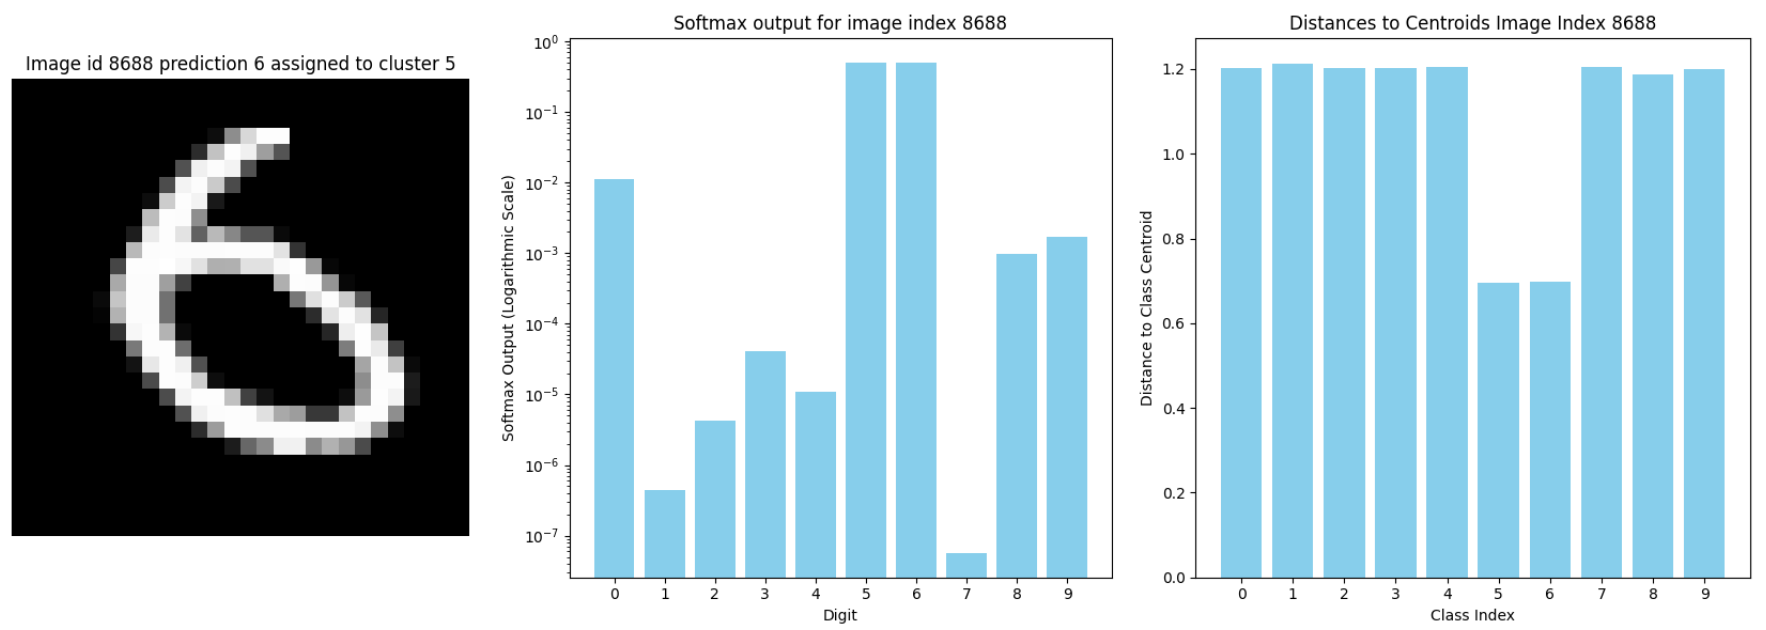
\includegraphics[width=0.99\columnwidth]{Figures/ImageID8688_Softmax_Clustering.png}
    \caption{Left to right, MNIST Training Data Image ID 8688 digit 6, the network softmax output and the distances to class centroids, correctly classified as 6 and incorrectly clustered as 5. Notice that the y axis is not on logarithmic scale in this case.   
    }
\label{fig:ImageID8688_Softmax_Clustering}
\end{figure}

\begin{figure}[ht!]
    \centering
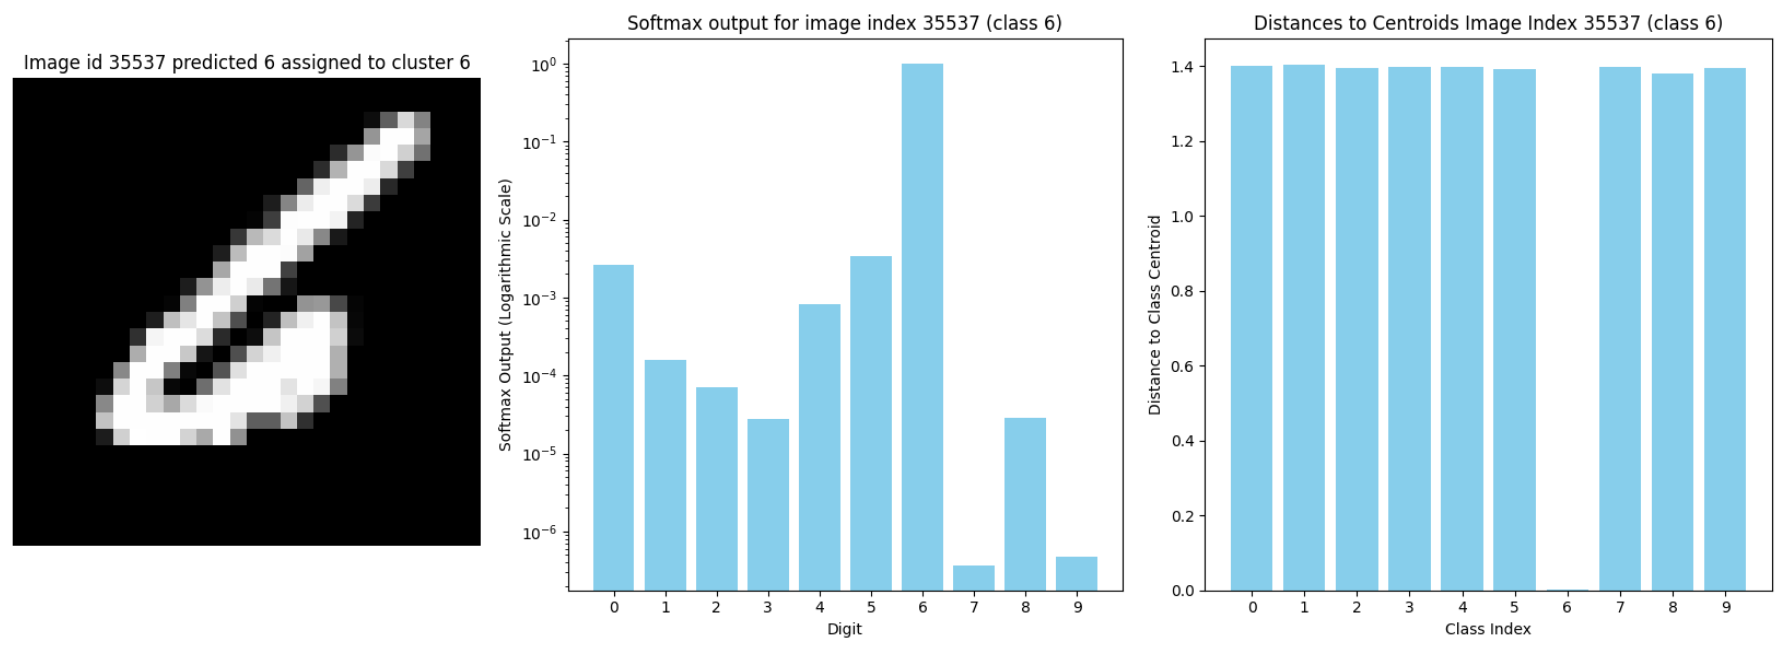
\includegraphics[width=0.99\columnwidth]{Figures/ImageID35537_Softmax_Clustering.png}
    \caption{Left to right, MNIST Training Data Image ID 35537 digit 6, the network softmax output and the distances to class centroids, correctly classified and correctly clustered as 6.     %MNIST_TRAINING_DATASET_ACC_RATIO_VS_THRESHOLD
    }
\label{fig:ImageID35537_Softmax_Clustering}
\end{figure}

The next example presents a contrasting case to the previous edge case. Figure \ref{fig:ImageID35537_Softmax_Clustering} shows a 6 where the softmax output assigns 0.993 probability to class 6, with all other classes receiving probabilities below 0.004 (the y axis is in log scale). The low entropy of the softmax output matches a clear separation of centroid distances. As before, there are differences in the histograms to be further investigated. 

In what follows, more than investigating individual examples case-by-case as in Figures \ref{fig:ImageID8688_Softmax_Clustering} and \ref{fig:ImageID35537_Softmax_Clustering}, the clustering will be used (and hence the differences in the histograms) to seek to identify general trends for entire classes represented by the cluster centroids.

\textbf{Varying Thresholds}: The uncertainty that the above edge case exemplifies suggests that it would be reasonable to classify the data point, not as a 6 or a 5, but as \textit{unknown}. In fact, it could be argued that in this case the classification should be ``5 or 6", in that the image is likely to be of one of those two digits, but it is not known which. It is now investigated, by varying the threshold used to define cluster membership, how certain examples may fall into an \textit{unknown} region of the clustering. An evaluation of how accuracy varies by changing this threshold and also how many examples fall into the \textit{unknown} region (retention), as well as the ratios of correct to incorrect predictions is performed. 

Figure~\ref{fig:MNIST_TRAINING_DATASET_ACC_RATIO_VS_THRESHOLD} depicts test set accuracy, retention (the percentage of examples belonging to the cluster hypersphere) and correct-to-incorrect ratio versus threshold (distance to predicted class centroid) for CIFAR/ViT (top) and MNIST/CNN (bottom). The y-left axis (percentage) ranges from 98.0\% to 100.0\% for both. For CIFAR/ViT, retention (blue) decreases from 100.0\% to 98.0\%, accuracy (green) increases from 99.4\% to 99.7\%, and the ratio (red) rises from 197:1 to 536:1 as the threshold decreases from 0.80 to 0.05. For MNIST/CNN, retention decreases from 100.0\% to 92.0\%, accuracy increases from 98.0\% to 99.0\%, and the ratio rises from 64:1 to 632:1 over the same threshold range. The ViT created more compact clusters, noting the ViT has 2 orders of magnitude more parameters than the CNN.

%The ViT/CIFAR-10 plot shows a tighter clustering on the y-left axis, with retention and accuracy varying within a 2.0\% range, compared to a 8.0\% range for CNN/MNIST, indicating the ViT architecture created more compact clusters, noting the ViT has 2 orders of magnitude more parameters than the CNN architecture.

\begin{figure}[ht!]
    \centering
    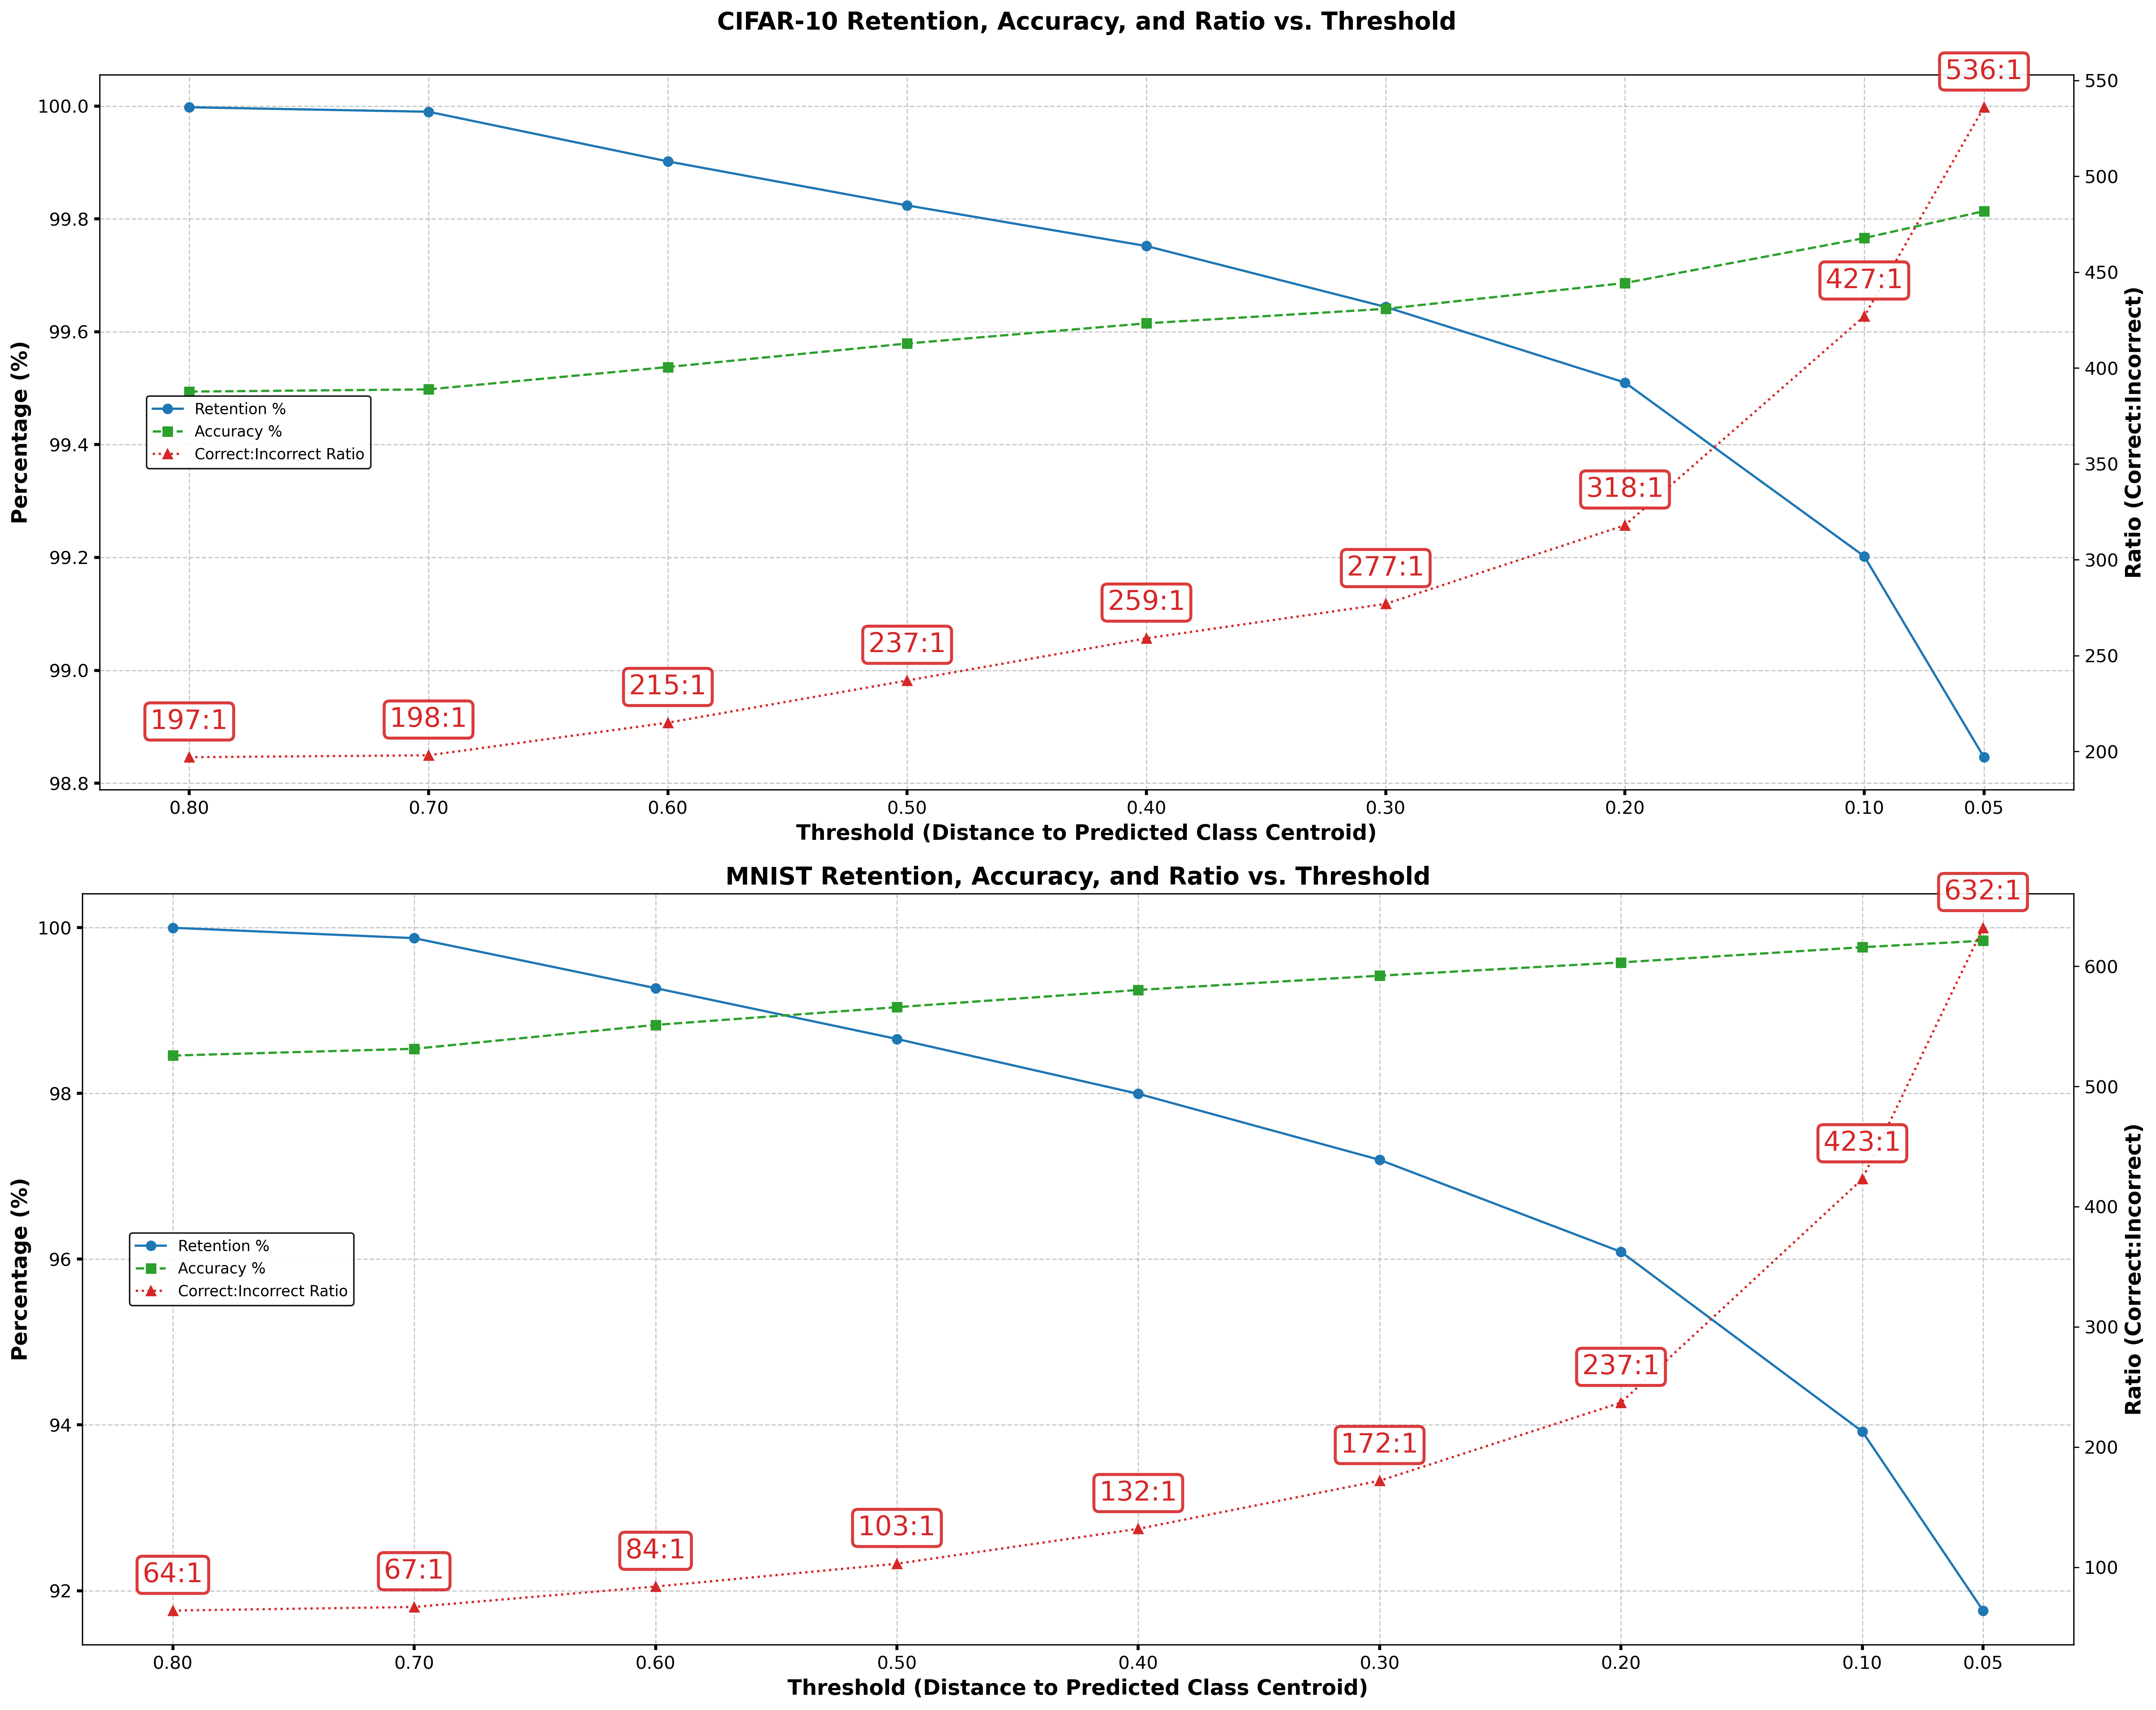
\includegraphics[width=0.99\columnwidth]{Figures/cifar10_mnist_retention_accuracy_ratio_vs_threshold.png}
    \caption{Retention, accuracy and correct-incorrect ratio vs Threshold ViT trained on CIFAR-10 and CNN trained on MNIST where the training dataset results are shown. The red plot represents the ratio of correct to incorrect predictions across all classes at given thresholds e.g. for CNN/MNIST at threshold 0.8 the ratio is 64:1, at threshold 0.05 the ratio is 632:1. The green plot is accuracy at every threshold e.g. at threshold 0.8 the accuracy is approximately 98.5\%, 64/(64+1), and at threshold 0.05 the accuracy is approximately 100\%, 632/(632+1). The blue plot represents the percentage of correct predictions that are being discarded as the threshold decreases e.g. at threshold 0.8 all correct predictions are kept while at threshold 0.05 over 8\% of the correct predictions are discarded i.e. classed as \textit{unknown}.}
\label{fig:MNIST_TRAINING_DATASET_ACC_RATIO_VS_THRESHOLD}
\end{figure}


\textbf{Class Average Softmax to K-Means Centroids}

\begin{table}[htbp]
\centering
\caption{Euclidean Distances between Class Average Softmax and K-Means Centroids}
\label{tab:diff_softmax_avg_dist_to_centroids}
\begin{tabular}{|c|c|}
\hline
Class & Distance \\
\hline
0 & 1.1694e-14 \\
\hline
1 & 1.0959e-14 \\
\hline
2 & 6.7639e-15 \\
\hline
3 & 1.7808e-14 \\
\hline
4 & 7.7425e-15 \\
\hline
5 & 1.3045e-04 \\
\hline
6 & 2.3118e-04 \\
\hline
7 & 1.3083e-14 \\
\hline
8 & 1.4139e-04 \\
\hline
9 & 1.2047e-14 \\
\hline
\end{tabular}
\end{table}

After running the K-Means clustering algorithm, initialised with the  average softmax outputs for each class, we obtain cluster centroids. We are interested in knowing how much the average softmax outputs moved from their initial position. 

Table \ref{tab:diff_softmax_avg_dist_to_centroids} presents the Euclidean distances between the average softmax outputs and the K-Means centroids for each digit class (0-9). For most digit classes (0, 1, 2, 3, 4, 7, 9), the Euclidean distances are extremely small, on the order of 1e-14 to 1e-15, indicating that the average softmax outputs are very close to the centroids obtained from the K-Means clustering algorithm. However, for digit classes 5, 6, and 8, the Euclidean distances are slightly larger, on the order of 1e-4, suggesting a minor difference between the average softmax outputs and the K-Means centroids for these specific classes, which indicates the class predictions for 5, 6 and 8 are not as closely clustered i.e. there is more "movement" from the softmax average to the final centroid position in the simplex.
% Plot created manually from MNIST and CIFAR10 plots created by function plot_accuracy_vs_distance_linear_fit
% Take 2
% repo: git@github.com:dsikar/IJCNN-2025.git
% file: scripts/hypersphere.py
% commit 06ce13ff908c33417afd27f4ad1fb9cb398bebd9
% TODOS
% 1. remove green accuracy labels
% 2. Improve caption
% 3. Create CIFAR-10 plot


%%%%%%%%%%%%%%%%%%%%%%%%%%%%%%%%%%%%%%%%%
% MISCLASSIFIED CHARACTERS MIN AND AVGS %
%%%%%%%%%%%%%%%%%%%%%%%%%%%%%%%%%%%%%%%%%

\textbf{Out-of-distribution Data:} Predictions for in-distribution data are expected to fall closer to class centroids, and predictions for out-of-distribution data further away. To study out-of-distribution data predictions, the English Handwritten Characters dataset (\cite{deCampos09}) (separating digits from alphabetic characters for the sake of analysis), and the CIFAR-10 dataset are \textit{MNISTified}. %by adapting the number of channels and ratio to conform to our CNN architecture. Figure \ref{fig:closest_alphabetic_characters_to_each_digit} shows which characters are nearest to each MNIST/CNN digit class centroid and also the average distance from the given class centroid (observing upper and lower case). For example, the lower case \textit{z} character shown (third from left) is among all alphabetic characters the nearest to centroid of digit class 2 (0.00893), where the average lower case \textit{z} is 0.20964 distance units away. Characters lower case \textit{b}, upper case \textit{B} and lower case \textit{a} show strong resemblance to digits \textit{6}, \textit{8} and \textit{9}, respectively. This is reflected in the clustering of the alphabetic dataset. Notice that no further training or fine-tuning of the CNN took place here. MNIST/CNN was only used for inference given the new character data set. The interest is in identifying, in the case of out-of-distribution data, how reasonable a prediction may be on average (not individual cases), as in the case of lower case \textit{z} above, and which predictions should fall in the \textit{unknown} region. 

\begin{figure}[ht!]
    \centering
    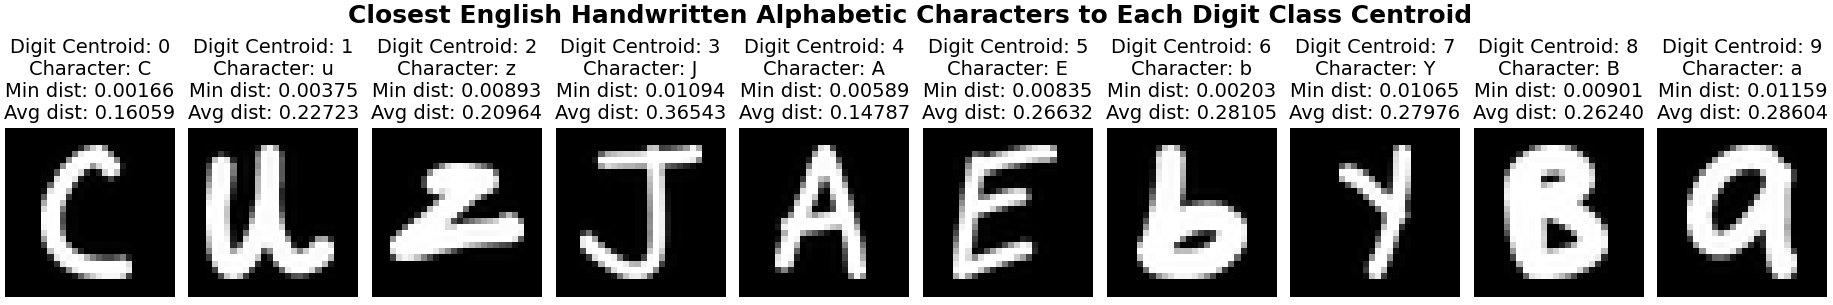
\includegraphics[width=0.99\columnwidth]{Figures/closest_alphabetic_characters_to_each_digit.png}
    \caption{English Handwritten Alphabetic Characters nearest distance and example, and averages}
\label{fig:closest_alphabetic_characters_to_each_digit}
\end{figure}

%%%%%%%%%%%%%%%%%%%%%%%%%%%%%%%
% MNISTified CIFAR10 EXAMPLES %
%%%%%%%%%%%%%%%%%%%%%%%%%%%%%%%
% removed for lack of space
% Figure \ref{fig:english_handwritten_characters_alphabetic_softmax_averages} shows examples of the \textit{MNISTified} CIFAR-10 dataset. As expected, the examples bear no resemblance to digits, which as we shall see is reflected in the clustering. In this case, one would expect all examples to be classified as \textit{unknown}.

% % plot_mnistified_samples(train_ds, cifar10_classes, convert_cifar10_to_mnist_format, filename='figures/mnistified_cifar10.png', save_flag=True)
% \begin{figure*}[ht!]
%     \centering
%     \includegraphics[width=0.99\textwidth]{Figures/ThresholdAnalysis/mnistified_cifar10.png}
%     \caption{MNISTified CIFAR10 Dataset Examples}
% \label{fig:english_handwritten_characters_alphabetic_softmax_averages}
% \end{figure*}

Table~\ref{tab:threshold_percentages} shows dataset percentages that fall below or at/above threshold with varying thresholds. For example, for threshold 0.8, all datasets except \textit{MNISTified} CIFAR-10 have 100\% of the examples below threshold. At the lowest threshold of 0.05, CIFAR-10 has the highest percentage of examples below threshold, indicating the tightest clustering, followed by MNIST, where the number of in-cluster examples starts dropping significantly at 0.3 threshold. The \textit{MNISTified} English Handwritten Digits are more tightly clustered than the English Alphabetical Characters, as the former bears a closer resemblance to the MNIST dataset, and the latter have no equivalent labels in the MNIST dataset and consequently all predictions are technically incorrect. It is noted that for the \textit{MNISTified} CIFAR-10, another case of all predictions being incorrect by default, and bearing no resemblance whatsoever to digits, has 97\% of examples rejected (excluded from all the clusters) at a threshold of 0.05. %The implication is there exist examples that bear no resemblance to digits, still classified by the neural network with a high degree of confidence, however, centroid proximity does increase the likelihood that the prediction is correct for in-distribution data.

\begin{table}[ht]
\centering
\caption{Percentage of examples below and at or above thresholds for distance to predicted class centroid across five datasets. Total examples: CIFAR-10 (50,000), MNIST (60,000), MNISTified English Handwritten Digits (550), MNISTified English Handwritten Alphabetical Characters (2,860), MNISTified CIFAR-10 (50,000).}
\label{tab:threshold_percentages}
\scriptsize
\begin{tabular*}{\textwidth}{@{\extracolsep{\fill}} c *{10}{S[table-format=3.1]}}
\toprule
 & \multicolumn{2}{c}{CIFAR-10} & \multicolumn{2}{c}{MNIST} & \multicolumn{2}{c}{Eng. Digits} & \multicolumn{2}{c}{Eng. Alphabetical} & \multicolumn{2}{c}{MNISTified CIFAR-10} \\
\cmidrule(lr){2-3} \cmidrule(lr){4-5} \cmidrule(lr){6-7} \cmidrule(lr){8-9} \cmidrule(lr){10-11}
Threshold & {Below} & {At/Above} & {Below} & {At/Above} & {Below} & {At/Above} & {Below} & {At/Above} & {Below} & {At/Above} \\
\midrule
0.8  & 100.0 & 0.0  & 100.0 & 0.0  & 100.0 & 0.0  & 100.0 & 0.0  & 98.2  & 1.8  \\
0.7  & 100.0 & 0.0  & 99.9  & 0.1  & 99.3  & 0.7  & 97.4  & 2.6  & 85.5  & 14.5 \\
0.6  & 99.9  & 0.1  & 99.3  & 0.7  & 96.5  & 3.5  & 90.2  & 9.8  & 67.4  & 32.6 \\
0.5  & 99.8  & 0.2  & 98.7  & 1.3  & 93.1  & 6.9  & 83.0  & 17.0 & 52.6  & 47.4 \\
0.4  & 99.8  & 0.2  & 98.0  & 2.0  & 89.3  & 10.7 & 75.0  & 25.0 & 39.1  & 60.9 \\
0.3  & 99.6  & 0.4  & 97.2  & 2.8  & 86.0  & 14.0 & 67.2  & 32.8 & 27.2  & 72.8 \\
0.2  & 99.5  & 0.5  & 96.1  & 3.9  & 81.6  & 18.4 & 58.0  & 42.0 & 16.5  & 83.5 \\
0.1  & 99.2  & 0.8  & 93.9  & 6.1  & 72.4  & 27.6 & 47.0  & 53.0 & 6.9   & 93.1 \\
0.05 & 98.8  & 1.2  & 91.8  & 8.2  & 67.8  & 32.2 & 38.7  & 61.3 & 3.0   & 97.0 \\
\bottomrule
\end{tabular*}
\end{table}

Figure~\ref{fig:Exclusion_Rate_vs_Threshold} shows the relationship between distance thresholds (x-axis) and exclusion percentages (y-axis). Five datasets are represented: CIFAR-10 (blue), MNIST (green), MNISTified English Digits (purple), MNISTified English Alphabetical (red), and MNISTified CIFAR-10 (yellow), with dataset counts indicated in parentheses. The x-axis ranges from 0.80 to 0.05, representing decreasing threshold values for the distance to predicted class centroid. The y-axis shows percentage values from 0\% to 100\%. MNISTified CIFAR-10 exhibits the highest exclusion rates across all thresholds. The MNISTified English Alphabetical dataset shows moderate exclusion rates (up to 61\%), while MNISTified English Digits demonstrates lower exclusion rates (up to 32\%). Both MNIST and CIFAR-10 maintain minimal exclusion rates below 10\% across all thresholds, with CIFAR-10 showing the lowest values overall, remaining under 1\%. 

\begin{figure}[ht!]
    \centering
    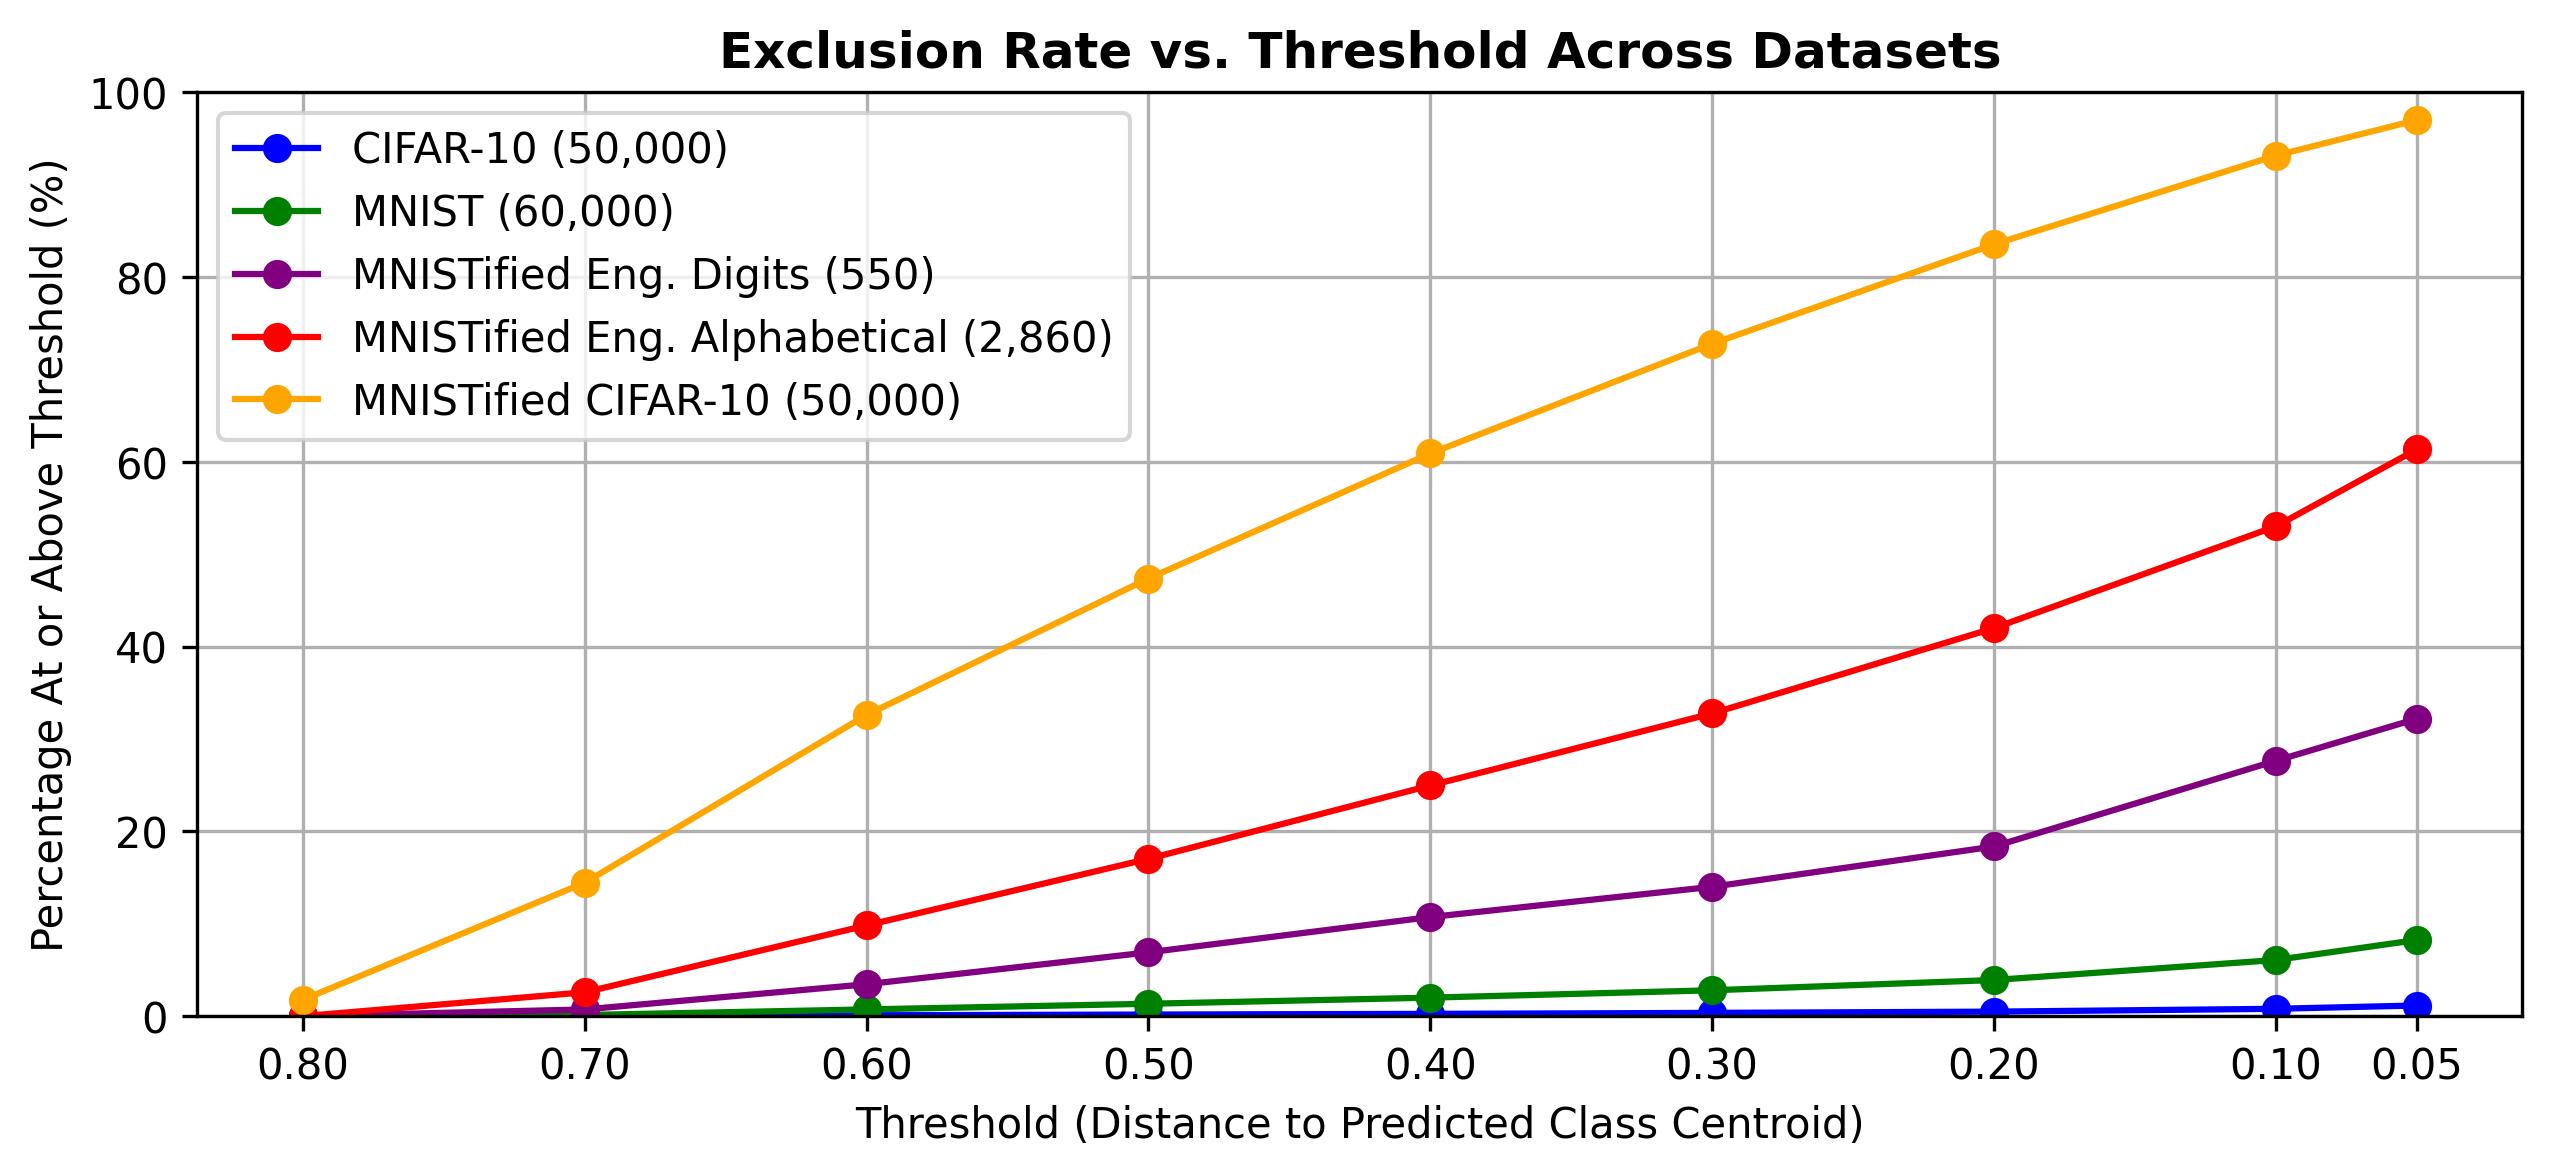
\includegraphics[width=0.99\columnwidth]{Figures/Exclusion_Rate_vs_Threshold.png}
    \caption{Percentage of examples at or above thresholds for distance to predicted class centroid across five datasets, showing higher exclusion rates for English Alphabetical Characters and MNISTified CIFAR-10. Total examples: CIFAR-10 (50,000), MNIST (60,000), Eng. Digits (550), Eng. Alphabetical (2,860), MNISTified CIFAR-10 (50,000).}
\label{fig:Exclusion_Rate_vs_Threshold}
\end{figure}

\begin{table}[ht]
\centering
\small
\caption{Density of points (\(N_k\), \(\rho_k\)) in 10-dimensional spherical shells and inner sphere, based on distance to predicted class centroid. Higher densities in outer shells for English Alphabetical Characters and MNISTified CIFAR-10 indicates greater exclusion. Total examples: CIFAR-10 (50,000), MNIST (60,000), Eng. Digits (550), Eng. Alphabetical (2,860), MNISTified CIFAR-10 (50,000).}
\label{tab:density}
\scriptsize
\begin{tabular}{@{} l l S[table-format=1.5e-1] *{5}{cc} @{}}
\toprule
 & & & \multicolumn{2}{c}{CIFAR-10} & \multicolumn{2}{c}{MNIST} & \multicolumn{2}{c}{Eng. Digits} & \multicolumn{2}{c}{Eng. Alphabetical} & \multicolumn{2}{c}{M'fied CIFAR-10} \\
\cmidrule(lr){4-5} \cmidrule(lr){6-7} \cmidrule(lr){8-9} \cmidrule(lr){10-11} \cmidrule(lr){12-13}
{Shell} & {Radii} & {Volume} & {$N_k$} & {$\rho_k$} & {$N_k$} & {$\rho_k$} & {$N_k$} & {$\rho_k$} & {$N_k$} & {$\rho_k$} & {$N_k$} & {$\rho_k$} \\
\midrule
1 & 0.7--0.8 & 2.01786e-1 & 4 & 2.0e1 & 75 & 3.7e2 & 4 & 2.0e1 & 74 & 3.7e2 & 6336 & 3.1e4 \\
2 & 0.6--0.7 & 5.6616e-2 & 44 & 7.8e2 & 362 & 6.4e3 & 15 & 2.6e2 & 207 & 3.7e3 & 9077 & 1.6e5 \\
3 & 0.5--0.6 & 1.29295e-2 & 39 & 3.0e3 & 368 & 2.8e4 & 19 & 1.5e3 & 206 & 1.6e4 & 7379 & 5.7e5 \\
4 & 0.4--0.5 & 2.22299e-3 & 36 & 1.6e4 & 397 & 1.8e5 & 21 & 9.4e3 & 227 & 1.0e5 & 6767 & 3.0e6 \\
5 & 0.3--0.4 & 2.52346e-4 & 54 & 2.1e5 & 478 & 1.9e6 & 18 & 7.1e4 & 223 & 8.8e5 & 5934 & 2.4e7 \\
6 & 0.2--0.3 & 1.47973e-5 & 67 & 4.5e6 & 666 & 4.5e7 & 24 & 1.6e6 & 264 & 1.8e7 & 5383 & 3.6e8 \\
7 & 0.1--0.2 & 2.60882e-7 & 154 & 5.9e8 & 1301 & 5.0e9 & 51 & 2.0e8 & 315 & 1.2e9 & 4802 & 1.8e10 \\
8 & 0.05--0.1 & 2.54767e-10 & 178 & 7.0e11 & 1296 & 5.1e12 & 25 & 9.8e10 & 238 & 9.3e11 & 1919 & 7.5e12 \\
Inner & $\leq$0.05 & 2.49039e-13 & 49423 & 2.0e17 & 55056 & 2.2e17 & 373 & 1.5e15 & 1106 & 4.4e15 & 1513 & 6.1e15 \\
\bottomrule
\end{tabular}
\end{table}


\begin{figure}[ht]
    \centering
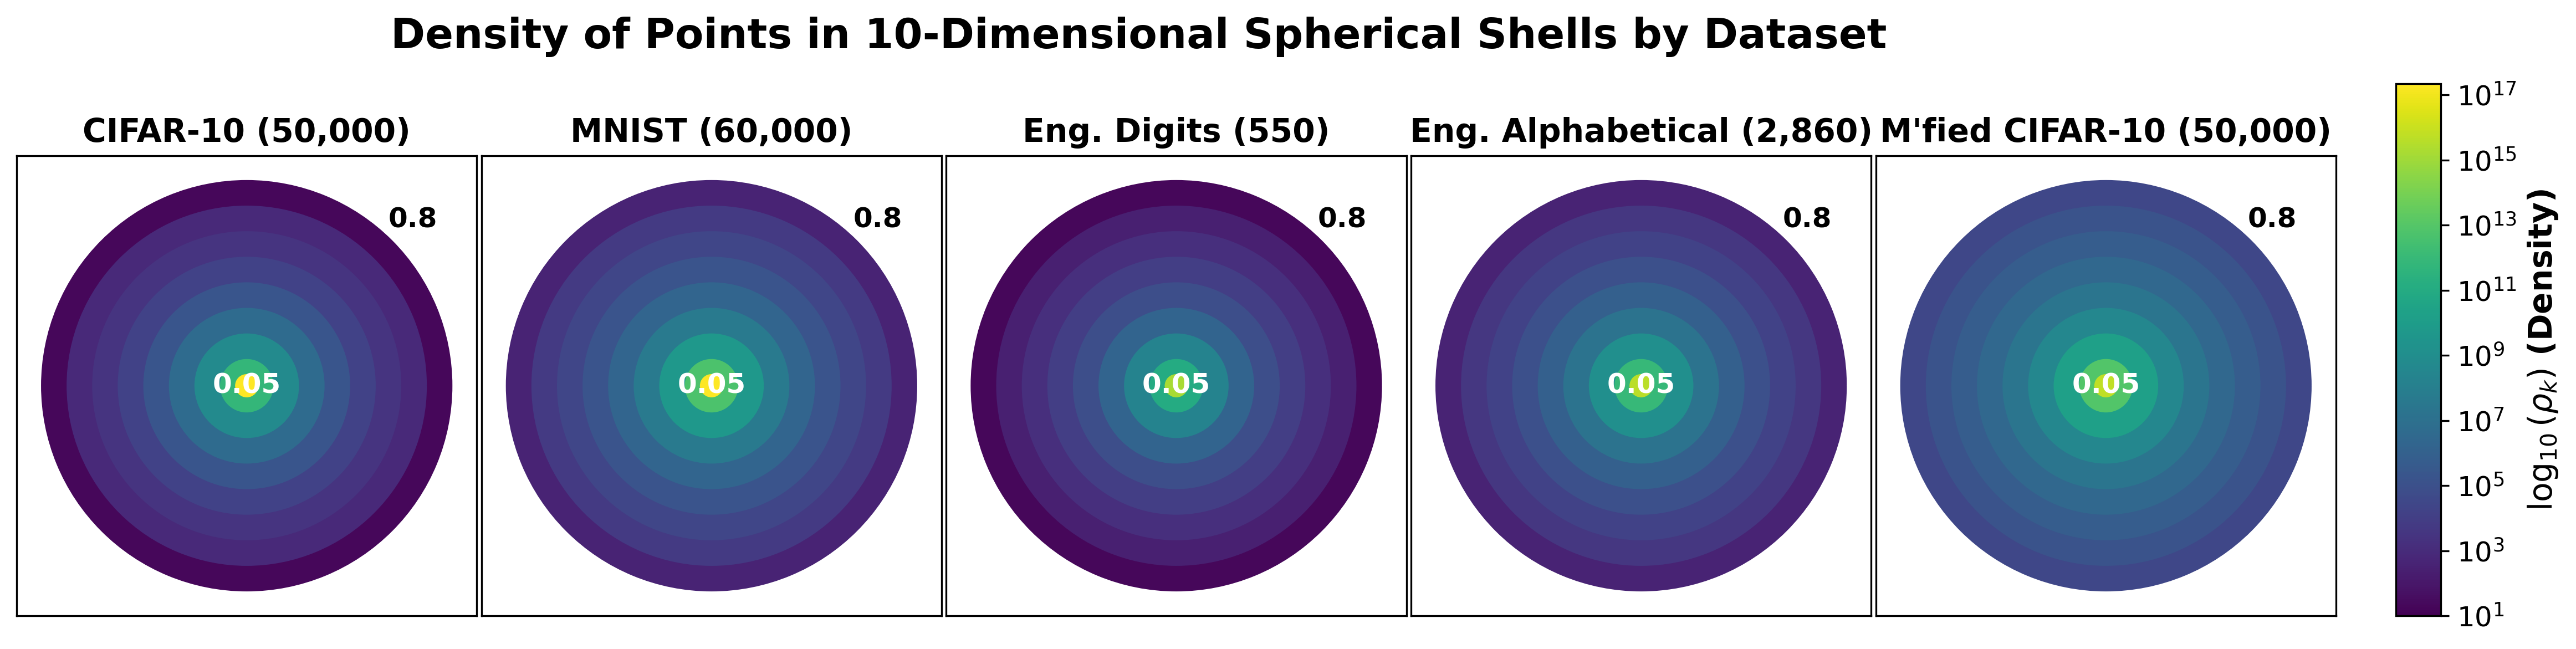
\includegraphics[width=0.99\columnwidth]{Figures/density_rings.png}
\caption{Density of points in 10-dimensional spherical shells, visualized as concentric rings. Color intensity represents $\log_{10}(\rho_k)$, with brighter colors indicating higher density. English Alphabetical Characters and MNISTified CIFAR-10 show higher density in outer shells, reflecting greater exclusion. Total examples: CIFAR-10 (50,000), MNIST (60,000), Eng. Digits (550), Eng. Alphabetical (2,860), MNISTified CIFAR-10 (50,000).}
\label{fig:density_rings}
\end{figure}

\textbf{Cluster Density}: Figure~\ref{fig:density_rings} presents a concentric ring visualisation of the density of points (\(\rho_k\)) in 10-dimensional spherical shells, defined by distance thresholds to the predicted class centroid [0.7--0.8, 0.6--0.7, 0.5--0.6, 0.4--0.5, 0.3--0.4, 0.2--0.3, 0.1--0.2, 0.05--0.1] and an inner sphere (\(\leq 0.05\)), across five datasets: CIFAR-10 (50,000 examples), MNIST (60,000 examples), English Handwritten Digits (550 examples), English Handwritten Alphabetical Characters (2,860 examples), and MNISTified CIFAR-10 (50,000 examples). The figure, a row of 5 subplots with a shared colourbar, encodes the density of softmax outputs in the 10-dimensional probability simplex, highlighting the higher exclusion rates (larger distances) for English Alphabetical Characters and MNISTified CIFAR-10. Next, the figure’s design is examined, its density patterns interpreted, and the implications and limitations of projecting high-dimensional data into a 2D representation addressed: each subplot represents a dataset, with eight concentric annuli corresponding to the shells and a central circle for the inner sphere. The radii are scaled to the thresholds (0.8 to 0.05), ensuring the outermost shell (0.7--0.8) is wider than the innermost (0.05--0.1), reflecting the hyperspherical geometry where volume scales as \(V_k \propto r^{10}\). Density (\(\rho_k\)) is mapped to a logarithmic colour scale, \(\log_{10}(\rho_k)\), using the \texttt{viridis} colormap, with dark purple for low density (\(\sim 10^1\)) and bright yellow for high density (\(\sim 10^{17}\)). This logarithmic scale accommodates the extreme density range, driven by the rapid volume decrease from \(2.02 \times 10^{-1}\) (Shell 1) to \(2.49 \times 10^{-13}\) (inner sphere). Annotations label the outermost ring (0.8) and inner sphere (0.05), and dataset names with example counts provide context. The shared colourbar, ranging from \(10^1\) to \(10^{17}\), ensures consistent density interpretation across subplots.

The figure emphasizes higher exclusion for English Alphabetical Characters and MNISTified CIFAR-10. For CIFAR-10 and MNIST, the outer rings are dark purple, indicating low density (\(\rho_1 = 2.0 \times 10^1\), \(\rho_2 = 7.8 \times 10^2\) for CIFAR-10; \(\rho_1 = 3.7 \times 10^2\), \(\rho_2 = 6.4 \times 10^3\) for MNIST), with few points at larger distances (\(N_1 = 4\), \(N_2 = 44\) for CIFAR-10; \(N_1 = 75\), \(N_2 = 362\) for MNIST). Their inner spheres are intensely yellow (\(\rho_9 = 2.0 \times 10^{17}\), \(N_9 = 49423\) for CIFAR-10; \(\rho_9 = 2.2 \times 10^{17}\), \(N_9 = 55056\) for MNIST), reflecting tight clustering near class centroids, consistent with low exclusion rates (1.2\% and 8.2\% at or above 0.05). The fine-tuned Vision Transformer (ViT) for CIFAR-10 and the convolutional neural network (CNN) optimized for MNIST produce confident predictions, concentrating softmax outputs in the inner sphere.

Conversely, English Alphabetical Characters and MNISTified CIFAR-10 display brighter outer rings, signalling higher density at larger distances. For English Alphabetical Characters, densities values like \(\rho_1 = 3.7 \times 10^2\), \(\rho_2 = 3.7 \times 10^3\), and \(\rho_4 = 1.0 \times 10^5\) appear as purple to green rings, driven by significant point counts (\(N_1 = 74\), \(N_2 = 207\), \(N_4 = 227\)). This reflects the MNIST CNN’s uncertainty in mapping letters to digit centroids, resulting in a high exclusion rate (61.3\% at or above 0.05). MNISTified CIFAR-10 shows even brighter green to yellow outer rings (\(\rho_1 = 3.1 \times 10^4\), \(\rho_2 = 1.6 \times 10^5\), \(\rho_4 = 3.0 \times 10^6\); \(N_1 = 6336\), \(N_2 = 9077\), \(N_4 = 6767\)), corresponding to the highest exclusion rate (97.0\% at or above 0.05), as the CNN misaligns non-digit CIFAR-10 images. English Handwritten Digits exhibit moderate outer-ring brightness (\(\rho_1 = 2.0 \times 10^1\), \(\rho_2 = 2.6 \times 10^2\); \(N_1 = 4\), \(N_2 = 15\)) and a less intense inner sphere (\(\rho_9 = 1.5 \times 10^{15}\), \(N_9 = 373\)), aligning with an intermediate exclusion rate (32.2\%).

Figure \ref{fig:density_rings} underscores the relationship between model performance and prediction geometry. The ViT’s robustness for CIFAR-10 and the CNN’s optimisation for MNIST yield dense inner spheres, indicating high confidence and low exclusion. The CNN is tested for out-of-distribution data (letters, non-digit images) and produces denser outer shells, suggesting potential for distance-based anomaly detection. However, the 2D projection simplifies the 10-dimensional probability simplex, where softmax outputs sum to 1, and the hyperspherical model assumes Euclidean distances, potentially skewing absolute density values. The extreme volume disparity (\(10^{-1}\) to \(10^{-13}\)) amplifies inner-sphere density, and the logarithmic colourmap may compress subtle outer-shell differences. In high dimensions, the ``curse of dimensionality'' concentrates volume near hypersphere surfaces, implying that even in-distribution points may lie in thin shells, though small distances (\(\leq 0.05\)) place them in the inner sphere.

\section{Conclusion and Future Work}

This chapter introduced a computationally lightweight approach for quantifying the confidence and reliability of predictions obtained from any neural network utilizing a softmax output layer. By clustering the softmax probability vectors and measuring the Euclidean distance between a given output and class centroids derived from the mean of correct predictions, we established a practical metric for assessing prediction confidence. A key finding is that this distance metric effectively serves as a proxy for confidence, enabling the system to identify potentially unreliable predictions and defer judgment by providing an ``unknown" answer, even when the original network has not been trained with that additional class, when a prediction falls outside a defined distance threshold. This threshold can be conservatively set based on the minimum distance observed for incorrect predictions within the training data. In practice, the choice of threshold will be domain dependent, although the analysis provided in Figure \ref{fig:Exclusion_Rate_vs_Threshold} may help an expert decide where the threshold should be set, based on the safety requirements or constraints of the application. The analysis provided in Figure \ref{fig:MNIST_TRAINING_DATASET_ACC_RATIO_VS_THRESHOLD} may also provide subsidies for the choice of threshold in the case of out-of-distribution data when expert knowledge is available comparing different data sets (or in the case where the data can be separated as with English digits and characters).

Our empirical evaluations, conducted using both Convolutional Neural Networks on MNIST and Vision Transformers on CIFAR-10, demonstrated consistency of results across different network architectures and datasets and the effectiveness of the proposed approach. The results confirmed that accurately predicted, in-distribution examples tend to cluster more tightly around their respective class centroids compared to misclassified or out-of-distribution examples, as shown in the analyses involving MNISTified datasets. The analysis of cluster density in the high-dimensional softmax space further reinforced results, showing higher densities in outer shells (larger distances) for OOD data and supporting the earlier results indicating robustness of the ViT model. We expect this method to offer a valuable tool in the analysis of trustworthiness of ML systems, flagging low-confidence predictions with minimal computational overhead. The approach is being evaluated on self-driving scenarios using the CARLA simulator.


% Note: Multiple abstract versions below - select one for final submission
% % Abstract, take 1
% % This paper demonstrates how to quantify uncertainty in regression models through a novel classification and clustering transform, enabling safety-critical autonomous systems to determine when predictions should not be trusted. While prior work has addressed regression uncertainty through Bayesian methods, ensemble techniques, and distributional predictions, these approaches typically require architectural modifications or computational overhead. We present an alternative approach that transforms regression problems into classification tasks, then leverages the geometric properties of the classification space to quantify uncertainty. By using k-means clustering on the softmax outputs of correctly classified examples we determine class centroids. The distance from new predictions to these centroids provides a principled uncertainty measure that requires no model retraining. We validate this approach on autonomous vehicle steering control in the CARLA simulator, where both CNN and Vision Transformer models are trained for steering angle prediction. By quantizing continuous steering angles into discrete bins, we show that distances to class centroids increase monotonically with visual perturbations (RGB pepper noise) and correlate linearly with lane invasion risk. Our method successfully predicts lane invasions before they occur by monitoring sequential predictions that exceed distance thresholds, enabling timely handover to human control. This classification-based uncertainty quantification offers a practical, computationally efficient alternative to existing methods while providing interpretable safety guarantees for regression-based autonomous systems.

% % Abstract, take 2
% % This paper demonstrates how to quantify uncertainty in regression via a classification and clustering transform. Prior work on regression uncertainty quantification (UQ) has primarily relied on Bayesian methods, ensembles, parametric distributions, or conformal prediction to estimate predictive variances and decompose epistemic/aleatoric sources (e.g., Gawlikowski et al., 2021; Lakshminarayanan et al., 2016; Zhou et al., 2025). While effective in domains like autonomous driving and medical imaging, these approaches often require architectural modifications or high computational overhead and lack direct, threshold-based confidence for sequential decision-making in safety-critical systems.

% % We propose a novel adaptation: quantizing continuous regression outputs (e.g., steering angles) into discrete classes, training classifiers, and seeding k-means centroids with softmax averages of correct predictions to define a bounded clustering space. Distances from new predictions to centroids serve as uncertainty proxies, with thresholds enabling "I don't know" flags for low-confidence cases.

% % We demonstrate a practical application in predicting lane invasions within a CARLA-simulated autonomous driving environment. Under increasing RGB pepper noise, centroid distances correlate linearly with lane deviations, allowing proactive detection of risky prediction sequences and timely handover to human control. Results show enhanced safety without eliminating all errors, generalizing to other regression-dependent systems like robotics or environmental forecasting. This method provides a lightweight, verifiable safety net for autonomous reliability.

% % Full title - for paper
% % When to Not Trust Your Regression Model: Quantifying Uncertainty for Autonomous System Safety

\chapter{Contribution 2 - Uncertainty Quantification in Regression Models via Classification and Clustering}

This chapter demonstrates how to quantify uncertainty in regression models through a novel classification and clustering transform, enabling safety-critical autonomous systems to determine when predictions should not be trusted. While prior work has addressed regression uncertainty through Bayesian methods, ensemble techniques, and distributional predictions, these approaches typically require architectural modifications or computational overhead. We present an alternative approach that transforms regression problems into classification tasks, then leverages the geometric properties of the classification space to quantify uncertainty. By using k-means clustering on the softmax outputs of correctly classified examples we determine class centroids. The distance from new predictions to these centroids provides a principled uncertainty measure that requires no model retraining. We validate this approach on autonomous vehicle steering control in the CARLA simulator, where both CNN and Vision Transformer models are trained for steering angle prediction. By quantizing continuous steering angles into discrete bins, we show that distances to class centroids increase monotonically with visual perturbations (RGB pepper noise) and correlate linearly with lane invasion risk. Our method successfully predicts lane invasions before they occur by monitoring sequential predictions that exceed distance thresholds, enabling timely handover to human control. This classification-based uncertainty quantification offers a practical, computationally efficient alternative to existing methods while providing interpretable safety guarantees for regression-based autonomous systems.

%%%%%%%%%%%%%%%%%%
%% INTRODUCTION %%
%%%%%%%%%%%%%%%%%%

\section{Introduction}

The deployment of machine learning models in autonomous systems has revolutionized fields ranging from self-driving vehicles to medical robotics, yet the critical question of when these systems should trust their own predictions remains largely unresolved. In safety-critical applications such as autonomous driving, medical diagnosis, and industrial automation, models must not only produce accurate predictions but also provide reliable estimates of their uncertainty (\cite{malinin2020regression, wibbeke2025evaluating, bigi2024prediction}). The consequences of overconfident predictions in such domains can be catastrophic, making uncertainty quantification not merely desirable but essential for safe autonomous operation (\cite{gawlikowski2021survey}).

Traditional regression models, while powerful for continuous prediction tasks, inherently lack mechanisms for expressing confidence in their outputs. Standard neural networks, for instance, provide only point estimates without any indication of prediction reliability (\cite{gawlikowski2021survey}). This limitation becomes particularly problematic in autonomous systems operating in dynamic, unpredictable environments where the model may encounter scenarios significantly different from its training distribution. Without proper uncertainty quantification, autonomous systems cannot make informed decisions about when to rely on model predictions, when to seek human intervention, or when to engage fail-safe mechanisms.

Existing approaches to uncertainty quantification in regression have made significant strides in addressing these challenges. Bayesian neural networks attempt to model parameter uncertainty by maintaining distributions over network weights rather than point estimates (\cite{dunger2025uncertainties}). Ensemble methods create multiple models with different initializations or training subsets, using the variance across predictions as an uncertainty measure (\cite{dunger2025uncertainties}). Monte Carlo dropout techniques approximate Bayesian inference by applying dropout during inference, generating multiple predictions to estimate uncertainty. Deep ensembles and evidential learning frameworks have also emerged as promising approaches for regression uncertainty quantification (\cite{wibbeke2025evaluating}).

However, these existing methods face several limitations that hinder their adoption in autonomous systems. Bayesian approaches, while theoretically principled, often suffer from computational overhead that makes real-time inference challenging (\cite{anand2025uncertainty}). Ensemble methods require training and maintaining multiple models, multiplying computational and memory requirements. Many uncertainty quantification techniques also struggle with calibration issues, where the predicted confidence levels do not accurately reflect true prediction reliability (\cite{gawlikowski2021survey}). Furthermore, the uncertainty estimates produced by these methods are often difficult to interpret, making it challenging for autonomous systems to translate uncertainty measures into actionable decisions.

The regulatory and safety requirements for autonomous systems demand not only accurate uncertainty estimates but also interpretable and computationally efficient methods that can operate within strict real-time constraints. Current approaches often fail to meet these dual requirements of accuracy and efficiency, creating a significant gap between theoretical advances in uncertainty quantification and practical deployment needs in autonomous systems.

\textbf{Regression-to-Classification Transformation}

An alternative approach to direct regression uncertainty quantification involves transforming continuous prediction problems into discrete classification tasks. This transformation, known as regression via classification (RvC), has gained significant attention in machine learning as it often improves model performance compared to standard regression approaches (\cite{stewart2022regression, berg2020deep}). The fundamental principle involves discretizing the continuous target variable into a finite set of non-overlapping bins or intervals, effectively converting the regression problem into a multi-class classification task (\cite{torgo1996regression, torgo1997regression}).

The transformation process requires careful consideration of how to partition the continuous output space. The most common approaches include \textbf{equal-width binning}, where the continuous range is divided into intervals of equal length, and \textbf{quantile-based binning}, where bins are created to contain approximately equal numbers of training examples (\cite{berg2020deep, barkov2024efficient}). More sophisticated methods employ adaptive quantization schemes that consider the underlying data distribution, with different strategies proving suitable for balanced data (linear quantization), long-tailed distributions (logarithmic quantization), or highly imbalanced scenarios (adaptive quantization) (\cite{xiong2023deep}).

The choice of discretization strategy creates a fundamental trade-off between classification accuracy and discretization error. Too few bins result in large quantization errors when recovering continuous target values, while too many bins lead to insufficient training examples per class, potentially degrading classification performance (\cite{berg2020deep}). Advanced approaches address this challenge through techniques such as kernel density integral quantization, which adaptively interpolates between uniform and quantile-based strategies (\cite{mccarter2024unmasking}), and optimal binning methods that satisfy constraints such as maintaining minimum samples per bin or enforcing monotonicity (\cite{huang2022mbct}).

Once classification is performed, the continuous regression estimate is typically recovered by computing the expected value over the predicted class probabilities weighted by bin centers or through more sophisticated distributional approaches (\cite{barkov2024efficient, keren2018calibrated}). This transformation approach has demonstrated particular success in computer vision tasks such as depth estimation, age estimation, and crowd counting, where classification formulations often outperform direct regression (\cite{fu2018deep, xiong2023deep}).

The regression-to-classification paradigm offers several advantages relevant to uncertainty quantification in autonomous systems. Classification models naturally provide probability distributions over discrete outcomes, which can serve as confidence measures. The discrete nature of the output space enables clearer decision boundaries and more interpretable confidence thresholds. Additionally, the vast arsenal of classification techniques, including ensemble methods and calibration approaches, becomes available for the transformed problem (\cite{guha2024conformal, pintea2023step}).

However, traditional regression-to-classification approaches still face limitations in autonomous system contexts. The binning process introduces discretization artifacts and requires careful hyperparameter tuning. The recovered continuous estimates may not adequately capture the uncertainty structure needed for safety-critical decisions. Most importantly, existing approaches do not provide principled methods for determining when the transformed model's predictions should be trusted or rejected in real-time autonomous operation.

This paper addresses these limitations by proposing a novel approach that transforms regression problems into classification tasks, then employs clustering techniques with centroid-based thresholds to provide computationally efficient and interpretable uncertainty estimates. Our method offers several key advantages: (1) computational efficiency suitable for real-time autonomous operation, (2) interpretable uncertainty measures based on geometric distance to learned cluster centroids, and (3) clear decision boundaries that enable autonomous systems to determine when predictions should be trusted or rejected.

The remainder of this paper is organized as follows: Section 2 reviews related work in uncertainty quantification for regression, Section 3 presents our clustering-based approach, Section 4 evaluates the method on benchmark datasets and autonomous system scenarios, and Section 5 concludes with implications for autonomous system safety and future research directions.

%%%%%%%%%%%%%%%%
% RELATED WORK %
%%%%%%%%%%%%%%%%

\section{Related Work}

This section reviews existing approaches to uncertainty quantification in regression models, with particular emphasis on methods relevant to autonomous systems. We organize our discussion around four key areas: traditional uncertainty quantification methods for regression, regression-to-classification transformation approaches, uncertainty estimation in classification models, and applications in safety-critical autonomous systems.

\textbf{Bayesian Approaches}

Bayesian neural networks (BNNs) represent one of the most principled approaches to uncertainty quantification in regression. Rather than learning point estimates for network parameters, BNNs maintain probability distributions over weights, enabling the model to express uncertainty about both parameters and predictions \cite{dunger2025uncertainties}. The predicted distribution directly contains probabilistic information that can be used for uncertainty estimation, providing a theoretically sound framework for distinguishing between aleatoric (data) and epistemic (model) uncertainty \cite{gawlikowski2021survey}.

However, BNNs face significant practical limitations, particularly in autonomous system deployments. The computational overhead associated with sampling from parameter distributions or performing variational inference makes real-time inference challenging \cite{anand2025uncertainty}. Additionally, the choice of prior distributions and approximation schemes can significantly impact the quality of uncertainty estimates, often requiring domain expertise and extensive hyperparameter tuning \cite{gawlikowski2021survey}.

\textbf{Ensemble Methods}

Ensemble approaches address uncertainty quantification by training multiple models with different initializations, data subsets, or architectural variations. The variance across ensemble predictions serves as an uncertainty measure, with higher variance indicating greater prediction uncertainty \cite{dunger2025uncertainties}. Deep ensembles, in particular, have demonstrated strong performance across various regression tasks by combining the predictions of multiple neural networks trained independently \cite{wibbeke2025evaluating}.

While ensemble methods often provide well-calibrated uncertainty estimates, they suffer from significant computational and memory overhead. Training and maintaining multiple models multiplies resource requirements, making deployment in resource-constrained autonomous systems problematic \cite{malinin2020regression}. Furthermore, ensemble methods primarily capture epistemic uncertainty through model diversity but may not adequately represent aleatoric uncertainty inherent in the data distribution.

\textbf{Monte Carlo Methods}

Monte Carlo dropout approximates Bayesian inference by applying dropout during both training and inference phases. By performing multiple forward passes with different dropout patterns, the method generates a distribution of predictions that can be used to estimate uncertainty \cite{wibbeke2025evaluating}. This approach offers a computationally efficient alternative to full Bayesian inference while maintaining some theoretical grounding.

Despite its efficiency advantages, Monte Carlo dropout has been shown to produce poorly calibrated uncertainty estimates, particularly when the dropout rate is not properly tuned for the specific task \cite{gawlikowski2021survey}. The method also struggles to capture epistemic uncertainty effectively when the model is confident but potentially wrong, a critical limitation for safety-critical applications.

\textbf{Evidential Learning}

Evidential deep learning frameworks attempt to learn the parameters of probability distributions directly, rather than learning point estimates. These methods place distributions over the parameters of the predictive distribution, enabling the quantification of epistemic uncertainty through the concentration of evidence \cite{malinin2020regression}. For regression tasks, evidential approaches often model the target distribution using parameterized families such as Gaussian or Student-t distributions.

While evidential methods show promise in providing interpretable uncertainty measures, they often require careful initialization and training procedures to avoid pathological solutions. The reliance on specific distributional assumptions may also limit their applicability to complex, multi-modal target distributions common in real-world autonomous system scenarios \cite{bigi2024prediction}.

% Next we examine regression-to-classification Transformation.

\textbf{Binning and Discretization Strategies}

The transformation of regression problems into classification tasks through discretization has a long history in machine learning, with early foundational work establishing the theoretical basis for this approach \cite{torgo1996regression, torgo1997regression}. The core challenge lies in effectively discretizing continuous target variables into meaningful bins that preserve the underlying structure while enabling effective classification.

\textbf{Equal-width binning} divides the continuous range into intervals of equal length, providing a simple and interpretable discretization scheme \cite{berg2020deep, barkov2024efficient}. However, for skewed distributions, this approach can result in bins with vastly different numbers of training examples, potentially leading to class imbalance issues that degrade classification performance.

\textbf{Quantile-based binning} addresses this limitation by creating bins that contain approximately equal numbers of training examples, ensuring balanced class distributions \cite{berg2020deep, barkov2024efficient}. While this approach improves classification balance, it may not respect the natural structure of the target distribution, potentially grouping dissimilar values together.

More sophisticated \textbf{adaptive quantization schemes} consider the underlying data distribution when determining bin boundaries. Different strategies prove suitable depending on the data characteristics: linear quantization for balanced data, logarithmic quantization for long-tailed distributions, and adaptive approaches for highly imbalanced scenarios \cite{xiong2023deep}. Advanced methods like kernel density integral quantization (KDI) adaptively interpolate between uniform and quantile-based strategies, automatically selecting appropriate discretization based on local data density \cite{mccarter2024unmasking}.

\textbf{Optimal Binning with Constraints}

Recent work has focused on developing principled approaches to binning that satisfy domain-specific constraints. Optimal binning methods use optimization techniques to maximize information-theoretic measures while respecting constraints such as minimum samples per bin, monotonicity requirements, or maximum number of bins \cite{huang2022mbct}. Mixed-integer programming approaches have been employed to identify optimal binning strategies that maximize measures like Jeffreys' Divergence, which reflects how well the discretized variable differentiates between classes \cite{barkov2024efficient}.

These constrained optimization approaches often provide superior discretization schemes compared to heuristic methods, but they introduce additional computational complexity and hyperparameter selection challenges. The trade-off between discretization quality and computational efficiency becomes particularly important in real-time autonomous system applications.

\textbf{Recovery Methods}

Once classification is performed on discretized targets, the continuous regression estimate must be recovered from the predicted class probabilities. The most common approach computes the expected value over predicted class probabilities weighted by bin centers or midpoints \cite{barkov2024efficient, keren2018calibrated}. More sophisticated recovery methods model the distribution within each bin, using training set statistics to refine the final continuous estimate.

Advanced recovery techniques include distributional approaches that maintain probability mass functions over bin boundaries, enabling more nuanced continuous predictions \cite{keren2018calibrated}. However, these methods may not significantly improve performance over simpler weighted averaging approaches, particularly when discretization is coarse.

% \subsection{Uncertainty Estimation in Classification}

\textbf{Calibration Methods}

The transformation from regression to classification enables the use of well-established classification uncertainty methods, but these require careful calibration to provide meaningful confidence estimates. Platt scaling, temperature scaling, and isotonic regression represent common post-hoc calibration techniques that adjust classifier outputs to better reflect true prediction confidence \cite{keren2018calibrated}.

\textbf{Bayesian binning} methods provide more sophisticated calibration by modeling the relationship between predicted probabilities and true frequencies using Bayesian inference \cite{huang2022mbct}. These approaches can capture complex calibration relationships but require additional validation data and computational overhead for training the calibration mappings.

\textbf{Conformal prediction} methods provide distribution-free uncertainty quantification by constructing prediction sets that contain the true target with a specified probability \cite{guha2024conformal}. Recent work has extended conformal prediction to regression-as-classification settings, enabling the construction of prediction intervals for continuous targets through the transformed classification framework.

The appeal of conformal methods lies in their theoretical guarantees: under the exchangeability assumption, conformal prediction sets achieve the desired coverage probability regardless of the underlying data distribution or model choice. However, the quality of prediction sets depends heavily on the choice of conformity scores and the effectiveness of the underlying classification model \cite{guha2024conformal}.

\textbf{Safety-Critical Requirements}

Autonomous systems operating in safety-critical environments require uncertainty quantification methods that satisfy stringent reliability, interpretability, and real-time performance requirements \cite{bigi2024prediction, wibbeke2025evaluating}. Traditional uncertainty methods often fail to meet these requirements due to computational overhead, calibration issues, or lack of interpretable confidence measures.

The automotive industry, in particular, has driven research into practical uncertainty quantification methods that can operate within the strict latency and reliability constraints of autonomous driving systems. Medical robotics and industrial automation present similar challenges, where prediction confidence directly impacts safety-critical decision making \cite{malinin2020regression}.

\textbf{Interpretability and Decision Making}

A critical limitation of many existing uncertainty quantification methods is their lack of interpretability, making it difficult for autonomous systems to translate uncertainty estimates into actionable decisions \cite{gawlikowski2021survey}. Rule-based systems for determining when to trust model predictions, when to seek human intervention, or when to engage fail-safe mechanisms require uncertainty measures that can be easily thresholded and interpreted by system designers.

Recent work has emphasized the need for uncertainty quantification methods that provide not just confidence estimates but also explanations for why particular predictions should or should not be trusted \cite{pintea2023step}. This requirement has driven interest in geometric and distance-based uncertainty measures that can be directly related to training data characteristics and model behavior.

\textbf{Motivation}

While existing uncertainty quantification methods provide valuable theoretical foundations and practical tools, they exhibit limitations such as computational complexity, Interpretability and the lack of a decision framework that hinder deployment in autonomous systems.

Our proposed clustering-based approach addresses these limitations by providing computationally efficient, interpretable uncertainty estimates based on geometric distance measures. By leveraging the regression-to-classification framework with centroid-based thresholds, our method enables clear decision boundaries for autonomous system safety while maintaining the computational efficiency required for real-time operation.

%%%%%%%%%%%
% METHODS %
%%%%%%%%%%%

\section{Methods}

This section presents our clustering-based uncertainty quantification approach for autonomous vehicle steering prediction. We describe the mathematical foundations of our method, the regression-to-classification transformation process, and the experimental setup using the CARLA autonomous driving simulator. Our approach addresses the critical need for computationally efficient and interpretable uncertainty estimation in safety-critical autonomous systems.

\textbf{Problem Formulation}

Consider a neural network trained for steering angle prediction in autonomous driving, where the model maps camera images $\mathbf{x} \in \mathbb{R}^{H \times W \times C}$ to steering angles $y \in \mathbb{R}$. Traditional regression approaches output a single continuous value without confidence estimates. Our method transforms this regression problem into a classification task, then applies geometric clustering analysis to quantify prediction uncertainty.

Let $f_{\theta}: \mathbb{R}^{H \times W \times C} \rightarrow \mathbb{R}^K$ represent our transformed neural network with parameters $\theta$, where $K$ is the number of discrete steering angle bins. The network outputs logits $\mathbf{z} = f_{\theta}(\mathbf{x}) = (z_1, z_2, \ldots, z_K)$, which are converted to probabilities via the softmax function:

$$p_i = \frac{e^{z_i}}{\sum_{j=1}^{K} e^{z_j}}$$

The resulting probability vector $\mathbf{p} = (p_1, p_2, \ldots, p_K)$ satisfies $\sum_{i=1}^K p_i = 1$ and represents the model's confidence distribution across steering angle classes.

\textbf{Discretization Strategy}

The continuous steering angle space is discretized into $K$ discrete bins corresponding to specific angular ranges. For autonomous driving applications, we implement three binning schemes based on CARLA's normalized control space:

\textbf{3-bin scheme:} $\{-0.065, 0.0, 0.065\}$ (Left, Straight, Right)

\textbf{5-bin scheme:} $\{-0.065, -0.015, 0.0, 0.015, 0.065\}$ (Hard Left, Soft Left, Straight, Soft Right, Hard Right)

\textbf{15-bin scheme:} $\{-0.065, -0.055, \ldots, -0.005, 0.0, 0.005, \ldots, 0.055, 0.065\}$ (Fine-grained steering control)

The number of bins must be odd to ensure a center bin corresponding to straight driving ($0.0°$ steering angle). Each configuration (15, 5, or 3 bins) represents a range of approximately $\pm 4.5°$ of the vehicle's $\pm 70°$ steering range, sufficient for lane-following without lane invasion on the experimental circuit.

\textbf{Model Architecture Adaptation}

The neural network architecture is modified to support classification outputs. The final linear layer changes from mapping to $\mathbb{R}^1$ (single continuous output) to mapping to $\mathbb{R}^K$ (K discrete class outputs). The loss function transitions from Mean Squared Error (MSE) for regression:

$$\mathcal{L}_{\text{MSE}} = \frac{1}{n} \sum_{i=1}^{n} (y_i - \hat{y}_i)^2$$

to Cross-Entropy Loss for classification:

$$\mathcal{L}_{\text{CE}} = -\frac{1}{n} \sum_{i=1}^{n} \sum_{j=1}^{K} y_{i,j} \log(p_{i,j})$$

where $y_{i,j}$ is the one-hot encoded true class and $p_{i,j}$ is the predicted probability for class $j$.

\textbf{Continuous Value Recovery}

For autonomous driving control, continuous steering angles must be recovered from discrete class predictions. The class index maps directly to the corresponding steering angle label. For example, for a classifier trained on data where steering angles were separated into 5 bins, a softmax output with highest score at index 1 (where indices go from 0 to 4), the corresponding label is $-0.015$, applying left steering to the vehicle.

\textbf{Clustering-Based Uncertainty Quantification Mathematical Framework}

Our uncertainty quantification method operates in the probability simplex defined by softmax outputs. Each prediction $\mathbf{p}$ lies within the $(K-1)$-dimensional standard simplex:

$$\Delta^{K-1} = \{\mathbf{p} \in \mathbb{R}^K : p_i \geq 0, \sum_{i=1}^K p_i = 1\}$$

This geometric constraint ensures that all cluster centroids and predictions exist within a bounded space, with maximum Euclidean distance between any two points bounded by $\sqrt{2}$, independent of dimensionality $K$.

\textbf{Centroid Calculation}

We compute class-specific centroids $\mathbf{C} = \{\mathbf{c}_1, \mathbf{c}_2, \ldots, \mathbf{c}_K\}$ from correct training predictions. For each class $k$, the centroid is calculated as:

$$\mathbf{c}_k = \frac{1}{|T_k|} \sum_{\mathbf{p} \in T_k} \mathbf{p}$$

where $T_k = \{\mathbf{p}_i : \arg\max(\mathbf{p}_i) = k \text{ and prediction is correct}\}$ represents the set of all correct predictions for class $k$.

\paragraph{Algorithm 1: Centroid Calculation}
\begin{verbatim}
Input: correct_predictions (n × K matrix of softmax outputs)
Output: centroids (K × K matrix of class centroids)

1. Initialize centroids ← zeros(K, K)
2. For each class k = 0 to K-1:
3.   indices ← where(argmax(correct_predictions, axis=1) == k)
4.   centroid ← mean(correct_predictions[indices], axis=0)
5.   centroids[k] ← centroid
6. Return centroids
\end{verbatim}

\textbf{Threshold Determination}

As a first pass, decision thresholds are determined using incorrect predictions from the training set. For each class $k$, we calculate the minimum distance from incorrect predictions to the corresponding centroid:

$$\tau_k = \min_{\mathbf{p} \in F_k} \|\mathbf{p} - \mathbf{c}_k\|_2$$

where $F_k = \{\mathbf{p}_i : \arg\max(\mathbf{p}_i) = k \text{ and prediction is incorrect}\}$ represents the set of incorrect predictions that were classified as class $k$. Fine-tuning and optimal threshold setting remains domain dependent.

\paragraph{Algorithm 2: Threshold Calculation}
\begin{verbatim}
Input: incorrect_predictions (n × K matrix), distances (n × 1 vector), 
true_classes (n × 1 vector)
Output: thresholds (K × 2 matrix of [threshold, class] pairs)

1. Initialize thresholds ← zeros(K, 2)
2. For each class k = 0 to K-1:
3.   class_distances ← distances[where(true_classes == k)]
4.   threshold ← min(class_distances)
5.   thresholds[k] ← [threshold, k]
6. Return thresholds
\end{verbatim}

\textbf{Decision Rule}

For a new prediction $\mathbf{p}_{\text{new}}$, we calculate distances to all centroids and apply the decision rule:

$$d_k = \|\mathbf{p}_{\text{new}} - \mathbf{c}_k\|_2$$

$$\text{predicted\_class} = \arg\max(\mathbf{p}_{\text{new}})$$

$$\text{decision} = \begin{cases}
\text{ACCEPT} & \text{if } d_{\text{predicted\_class}} < \tau_{\text{predicted\_class}} \\
\text{REJECT} & \text{otherwise}
\end{cases}$$

This geometric approach provides interpretable uncertainty measures: predictions closer to training centroids are more trustworthy, while predictions far from centroids indicate potential out-of-distribution inputs or model uncertainty.

\textbf{CARLA Simulation Environment Experimental Setup}

We conduct experiments using CARLA 0.9.13 (Car Learning to Act), an open-source autonomous driving simulator built on Unreal Engine \cite{dosovitskiy17}. CARLA provides realistic urban environments with dynamic weather, traffic, and pedestrian conditions, enabling controlled experimentation for autonomous driving algorithms.

The simulation configuration uses the Town04 figure-of-eight circuit. The route consists of 28 road segments following lane ID –2 (the second lane left-to-right, right-hand traffic). The vehicle is equipped with a front-facing RGB camera, whose mounting position and orientation are configurable and typically set at 1.5 units of distance above (along z axis) and 1.8 units of distance ahead (along x axis) of the vehicle's centre (waypoint). Weather conditions such as cloudiness, precipitation, and fog are controllable, as well as number of cars and pedestrians. The simulation runs in synchronous mode to ensure deterministic execution steps.

\textbf{Dataset Generation}

The dataset generation process is based on waypoint navigation. The vehicle follows predefined waypoints extracted from the town map mesh, identified by road\_id and lane\_id attributes. The figure-of-eight circuit is composed of waypoints spaced at 1-unit intervals for regression tasks and 3-unit intervals for classification tasks.

The steering algorithm computes the angular difference between the vehicle’s current orientation and the target waypoint orientation. This difference is applied as a steering correction to maintain lane-following behaviour, as defined by

\[
\mathrm{steering\_angle} = \mathrm{atan2}(\mathrm{target\_y} - \mathrm{vehicle\_y}, \mathrm{target\_x} - \mathrm{vehicle\_x}) - \mathrm{vehicle\_heading}
\]

During data collection, the system records RGB camera images (cropped and resized to 200×66 pixels), steering angle labels embedded in timestamped filenames, ground truth safety distances (measured as the perpendicular distance to the lane centerline), and lane invasion events (a distance greater than 0.85 units indicates a lane invasion). Each complete circuit lap produces approximately 28,000 labeled image–steering pairs under synchronous execution mode.

\textbf{Image Preprocessing}

Images undergo spatial cropping to remove sky regions and the vehicle hood, retaining only the pixels from y-coordinates 210 to 480. The cropped images are then resized to 200×66 pixels using bilinear interpolation to conform to the NVIDIA architecture requirements \cite{bojarski2016end}. Finally, RGB images are converted to the YUV color space following established autonomous driving practices \cite{lecun2004dave}, as YUV representation offers better perceptual similarity to human vision and improved performance in computer vision applications.

\textbf{Dataset Variants}

The regression variants include three configurations: \textbf{Vanilla}, which uses raw camera images with continuous steering angle targets; \textbf{Segmented}, which overlays lane segmentation markers on the images; and \textbf{Segmented with Fiducials}, which combines lane segmentation with fiducial markers.

For the classification variants, datasets are generated for each binning scheme (3, 5, and 15 bins). Two versions are produced for each scheme: \textbf{Unbalanced}, which preserves the natural steering angle distribution where straight driving predominates, and \textbf{Balanced}, in which images from minority classes are randomly duplicated to achieve equal class distributions.


\textbf{Neural Network Architecture}

We implement the NVIDIA end-to-end learning architecture \cite{bojarski2016end} adapted for both regression and classification tasks:

The implemented model follows the NVIDIA end-to-end learning architecture \cite{bojarski2016end}, adapted for both regression and classification tasks. The network consists of five convolutional layers followed by three fully connected layers and a single output layer. The convolutional block progressively increases the number of filters from 24 to 64 across five layers, employing kernel sizes of 5×5 and 3×3 with ELU activations and stride configurations designed to extract hierarchical spatial features from input images.  

The fully connected block maps the flattened feature representation through layers of 100, 50, and 10 neurons, each using ELU activations and dropout regularization with a rate of 0.1 to reduce overfitting. The final output layer consists of one neuron for regression tasks or \(K\) neurons for classification, where \(K \in \{3, 5, 15\}\) corresponds to the number of steering angle bins.  

Training is performed using the Adam optimizer with a learning rate of \(1\times10^{-5}\) and a batch size of 64 samples. Data are split randomly into 80\% for training and 20\% for validation. Early stopping is applied after six epochs without improvement in validation loss, with a maximum of 100 epochs. All experiments are executed on an NVIDIA GPU with CUDA acceleration.

In addition to the NVIDIA end-to-end convolutional architecture, a Vision Transformer (ViT) model is employed for comparative evaluation. The ViT is used directly for classification tasks, producing discrete steering angle predictions according to the chosen binning scheme. For regression tasks, the same model is adapted by replacing the final classification head with a single linear output neuron, enabling continuous steering angle estimation. This adaptation allows direct validation of the ViT’s capability to predict continuous steering values alongside the CNN-based baseline.

\textbf{Evaluation Metrics}

For regression tasks, performance is evaluated using the Mean Absolute Error (MAE), defined as  
\[
\text{MAE} = \frac{1}{n}\sum_{i=1}^{n}|y_i - \hat{y}_i|,
\]
and the Mean Squared Error (MSE), defined as  
\[
\text{MSE} = \frac{1}{n}\sum_{i=1}^{n}(y_i - \hat{y}_i)^2.
\]

For classification tasks, the primary metric is accuracy, representing the percentage of correct class predictions, complemented by per-class precision and recall to account for imbalanced datasets.

Uncertainty quantification is assessed through several additional metrics: the Accept Rate, measuring the percentage of predictions above a confidence threshold; the Reject Rate, representing the percentage below it; the Safety Margin, defined as the average distance to the decision boundary for accepted predictions; and the Lane Invasion Rate, which captures the frequency of lane violations during autonomous operation.


\textbf{Safety Assessment}

Lane invasion detection involves real-time monitoring of the vehicle's position relative to lane boundaries. Perpendicular distances exceeding 0.85 CARLA units trigger lane invasion events, indicating potential safety violations.

Distance-based safety integrates clustering-based uncertainty quantification with geometric safety measures. Predictions exhibiting high uncertainty (i.e., large centroid distances) are found to correlate with increased lane invasion risk, thereby validating the safety relevance of the proposed uncertainty estimates.

Fail-safe mechanisms are implemented for cases in which predictions are rejected due to high uncertainty. In such situations, the system can execute predefined responses, such as maintaining the current steering angle, requesting human intervention, or engaging emergency lane-keeping assistance.

This comprehensive methodology provides a principled framework for uncertainty-aware autonomous driving, combining regression-to-classification transformation with geometric clustering analysis to enable safe, interpretable decision-making in real-time autonomous systems.

%%%%%%%%%%%%%%%%%%%%%%%%%%%%
%% RESULTS AND DISCUSSION %%
%%%%%%%%%%%%%%%%%%%%%%%%%%%%

\section{Results And Discussion}

%%%%%%%%%%%%%%%%%%%%%
% REGRESSION MODELS %
%%%%%%%%%%%%%%%%%%%%%

\textbf{Regression Models}
\begin{longtable}{@{}lllllll@{}}
\toprule
Model Name & Dataset & Train Loss & Eval Loss & MAE & O MAE & D MAE \\
\midrule
\endfirsthead
\toprule
Model Name & Dataset & Train Loss & Eval Loss & MAE & O MAE & D MAE \\
\midrule
\endhead
RegCNNCUFid & Cont Unbal w/ Fids & 0.0000 & 0.0000 & N/A & 0.0036 & 0.0461 \\
RegCNNCU & Continuous Unbal & N/A & N/A & N/A & 0.0033 & 0.0588 \\
RgrViTCU & Continuous Unbal & 0.0002 & 0.0001 & 0.0076 & 0.0076 & 0.0399 \\
\bottomrule
\caption{Regression Model Performance}
\label{results:table_regression_models}
\end{longtable}

Table~\ref{results:table_regression_models} reports the performance of three regression models trained on the continuous unbalanced dataset. The columns are as follows: Train Loss and Eval Loss refer to the mean squared error on the training and evaluation sets, respectively; MAE is the mean absolute error computed during training; O MAE is the mean absolute error calculated over the combined training and evaluation sets; and D MAE is the mean absolute lateral deviation of the simulated vehicle from the centerline, measured during autonomous driving in the Town04 figure-of-eight loop. Where N/A appears, the corresponding value was not recorded during training.

The RegCNNCUFid model incorporates fiducial markers as input and achieved a D MAE of 0.0461, with an O MAE of 0.0036. The RegCNNCU model, which uses the same architecture without fiducials, obtained a slightly lower O MAE (0.0033) but a higher D MAE (0.0588). The difference in D MAE between these two models is small and may be attributed to statistical noise, as both values remain well below the operational threshold of 0.85, beyond which lane invasion would occur.

The RgrViTCU model, based on a ViT architecture, yielded an O MAE of 0.0076 and the lowest D MAE among the three (0.0399). Since MAE values were not recorded for the CNN-based models, comparisons across all models using that column are not possible. All D MAE values are within the bounds of acceptable simulated driving behavior, and the differences observed do not approach the threshold of operational relevance.

%%%%%%%%%%%%%%%%%%%%%%%%%
% CLASSIFICATION MODELS %
%%%%%%%%%%%%%%%%%%%%%%%%%

\textbf{Classification Models}
\begin{longtable}{@{}llllllll@{}}
\toprule
Model Name & Dataset & T Acc & T Loss & V Acc & V Loss & O Acc & D MAE \\
\midrule
\endfirsthead
\toprule
Model Name & Dataset & T Acc & T Loss & V Acc & V Loss & O Acc & D MAE \\
\midrule
\endhead
ClsCNN3bB & 3-bin Bal & 83.16\% & 0.3797 & 83.02\% & 0.3808 & 83.36\% & 0.0365 \\
ClsCNN3bU & 3-bin Unbal & 86.97\% & 0.3129 & 87.14\% & 0.3110 & 87.36\% & 0.0466 \\
ClsCNN5bB & 5-bin Bal & 87.45\% & 0.3001 & 86.92\% & 0.2975 & 87.70\% & 0.0491 \\
ClsCNN5bU & 5-bin Unbal & 92.87\% & 0.1993 & 93.03\% & 0.1928 & 93.18\% & 0.0753 \\
ClsCNN15bB & 15-bin Bal & 48.01\% & 1.0744 & 47.81\% & 1.0598 & 48.01\% & 0.0162 \\
ClsCNN15bU & 15-bin Unbal & 73.76\% & 0.7241 & 75.34\% & 0.6839 & 75.11\% & 0.0194 \\
ClsViT3bB & 3-bin Bal & N/A & 0.1875 & 97.15\% & 0.0960 & 97.97\% & 0.0462 \\
ClsViT3bU & 3-bin Unbal & N/A & 0.2625 & 91.93\% & 0.2075 & 92.50\% & 0.0397 \\
ClsViT5bB & 5-bin Bal & N/A & 0.1317 & 97.54\% & 0.0766 & 97.77\% & 0.0454 \\
ClsViT5bU & 5-bin Unbal & N/A & 0.1985 & 94.05\% & 0.1590 & 94.97\% & 0.0666 \\
ClsViT15bB & 15-bin Bal & N/A & 0.4012 & 92.92\% & 0.1984 & 93.86\% & 0.0925 \\
ClsViT15bU & 15-bin Unbal & N/A & N/A & N/A & N/A & 76.55\% & 0.0844 \\
\bottomrule
\caption{Classification Model Performance: training and self-driving, with quantized balanced and unbalanced datasets. The first row shows data for a CNN classifier trained on a 3-bin dataset - steering angles -0.065 (-4.55 degrees), 0 and 0.065 (4.55 degrees). The training accuracy is 83.17\%, the training loss 0.3739, the validation accuracy 83.02\%, the validation loss 0.3808, the overall accuracy when training and validation datasets are combined is 83.36\%. The distance mean average error (DMAE) is 0.0365, this is the average distance between the optimal middle-of-the-lane path and the vehicle path}
\label{results:classifier_models_results_table}
\end{longtable}

Table~\ref{results:classifier_models_results_table} presents the results for CNN and ViT models that were converted from regression models to perform classification, under three quantization schemes—3, 5, and 15 steering angle bins—and using either balanced or unbalanced datasets. The columns are as follows: T Acc and T Loss denote training accuracy and training loss; V Acc and V Loss are validation accuracy and validation loss; O Acc represents the overall accuracy across the full dataset (training and validation combined); and D MAE is the mean absolute error of the vehicle’s lateral deviation from the centerline. Entries marked N/A indicate that the corresponding values were not recorded during training. The D MAE values were computed through inference: after training, each model was deployed to drive autonomously around the Town04 figure-of-eight track, and its average distance from the intended trajectory was measured.

Among the CNN classifiers, ClsCNN5bU (trained on the unbalanced 5-bin dataset) achieved the highest overall accuracy (93.18\%), making it the best-performing CNN model. While its D MAE was slightly higher (0.0753), this remains well below the threshold (0.85 units) beyond which the vehicle would cross into an adjacent lane—meaning the deviation is not operationally significant and may be attributed to statistical noise. For the ViT models, ClsViT3bB (trained on the balanced 3-bin dataset) showed the strongest performance, with an overall accuracy of 97.97\% and a D MAE of 0.0462. In general, ViT models outperformed CNNs in both accuracy and driving precision, particularly on balanced datasets with coarser quantization. Given the low D MAE values across the board, most differences are unlikely to be practically significant in terms of simulated driving safety.

Overall Accuracy for CNN classifiers is consistently higher for models trained on unbalanced datasets, while the trend is inverted for ViT classifiers. This may be related to dataset sizes and network capacity, and is set as an investigative topic for future work.

%%%%%%%%%%%%%%%%%%%%%%%%%%%%%%%%%%%%%%%%%%%%%%%%%%%%%%%%%%
% BEST PERFORMING CLASSIFICATION MODEL INFERENCE RESULTS %
%%%%%%%%%%%%%%%%%%%%%%%%%%%%%%%%%%%%%%%%%%%%%%%%%%%%%%%%%%

\textbf{Best-Performing Classification Model Inference Results}

%%%%%%%%%%%%%%%%%%%%%%%%
% ClsCNN5binUnbalanced %
%%%%%%%%%%%%%%%%%%%%%%%%

\textbf{ClsCNN5binUnbalanced}

The ClsCNN5binUnbalanced model was trained on an unbalanced dataset containing five discrete steering angle bins corresponding to finer directional categories. The test set comprised 26,991 images, reflecting the distribution of steering angles where straight driving instances dominate.

The model achieved an overall classification accuracy of 93.18\% with a mean confidence of 0.9294. Class-wise performance indicates a concentration of predictive accuracy in the central bins, particularly for the straight and near-straight classes ($0.000$ and $\pm0.015$), which achieved F1-scores of 0.97 and 0.90–0.93, respectively. In contrast, the outermost steering bins ($\pm0.065$) show reduced recall values (0.36 and 0.57), indicating that sharp turning manoeuvres are less frequently detected. Precision for these outer bins remains moderate (0.80–0.87), suggesting limited false positives but an overall imbalance in sensitivity toward rare turning cases.

The macro-averaged precision, recall, and F1-score were 0.88, 0.76, and 0.80, respectively, consistent with class imbalance effects. These results suggest that the convolutional architecture retains strong predictive ability for dominant steering behaviours but exhibits degraded recall for infrequent sharp turns, emphasizing the impact of dataset imbalance on steering angle classification performance.


\begin{table}[htbp]
\centering
\begin{tabular}{@{}lcccc@{}}
\toprule
\textbf{Class} & \textbf{Precision} & \textbf{Recall} & \textbf{F1-Score} & \textbf{Support} \\
\midrule
$-0.065$ & 0.80 & 0.36 & 0.50 & 401 \\
$-0.015$ & 0.85 & 0.97 & 0.90 & 5,843 \\
$\phantom{-}0.000$ & 0.98 & 0.95 & 0.97 & 15,839 \\
$\phantom{-}0.015$ & 0.90 & 0.96 & 0.93 & 3,972 \\
$\phantom{-}0.065$ & 0.87 & 0.57 & 0.69 & 936 \\
\midrule
\textbf{Macro Avg} & \textbf{0.88} & \textbf{0.76} & \textbf{0.80} & \textbf{26,991} \\
\bottomrule
\end{tabular}
\caption{Classification performance results for the ClsCNN5binUnbalanced model. The model achieved an overall accuracy of 93.18\% with a mean confidence of 0.9294 across 26,991 test images.}
\label{tab:clf_report_ClsCNN5binUnbalanced}
\end{table}

\begin{figure}[H]
\centering
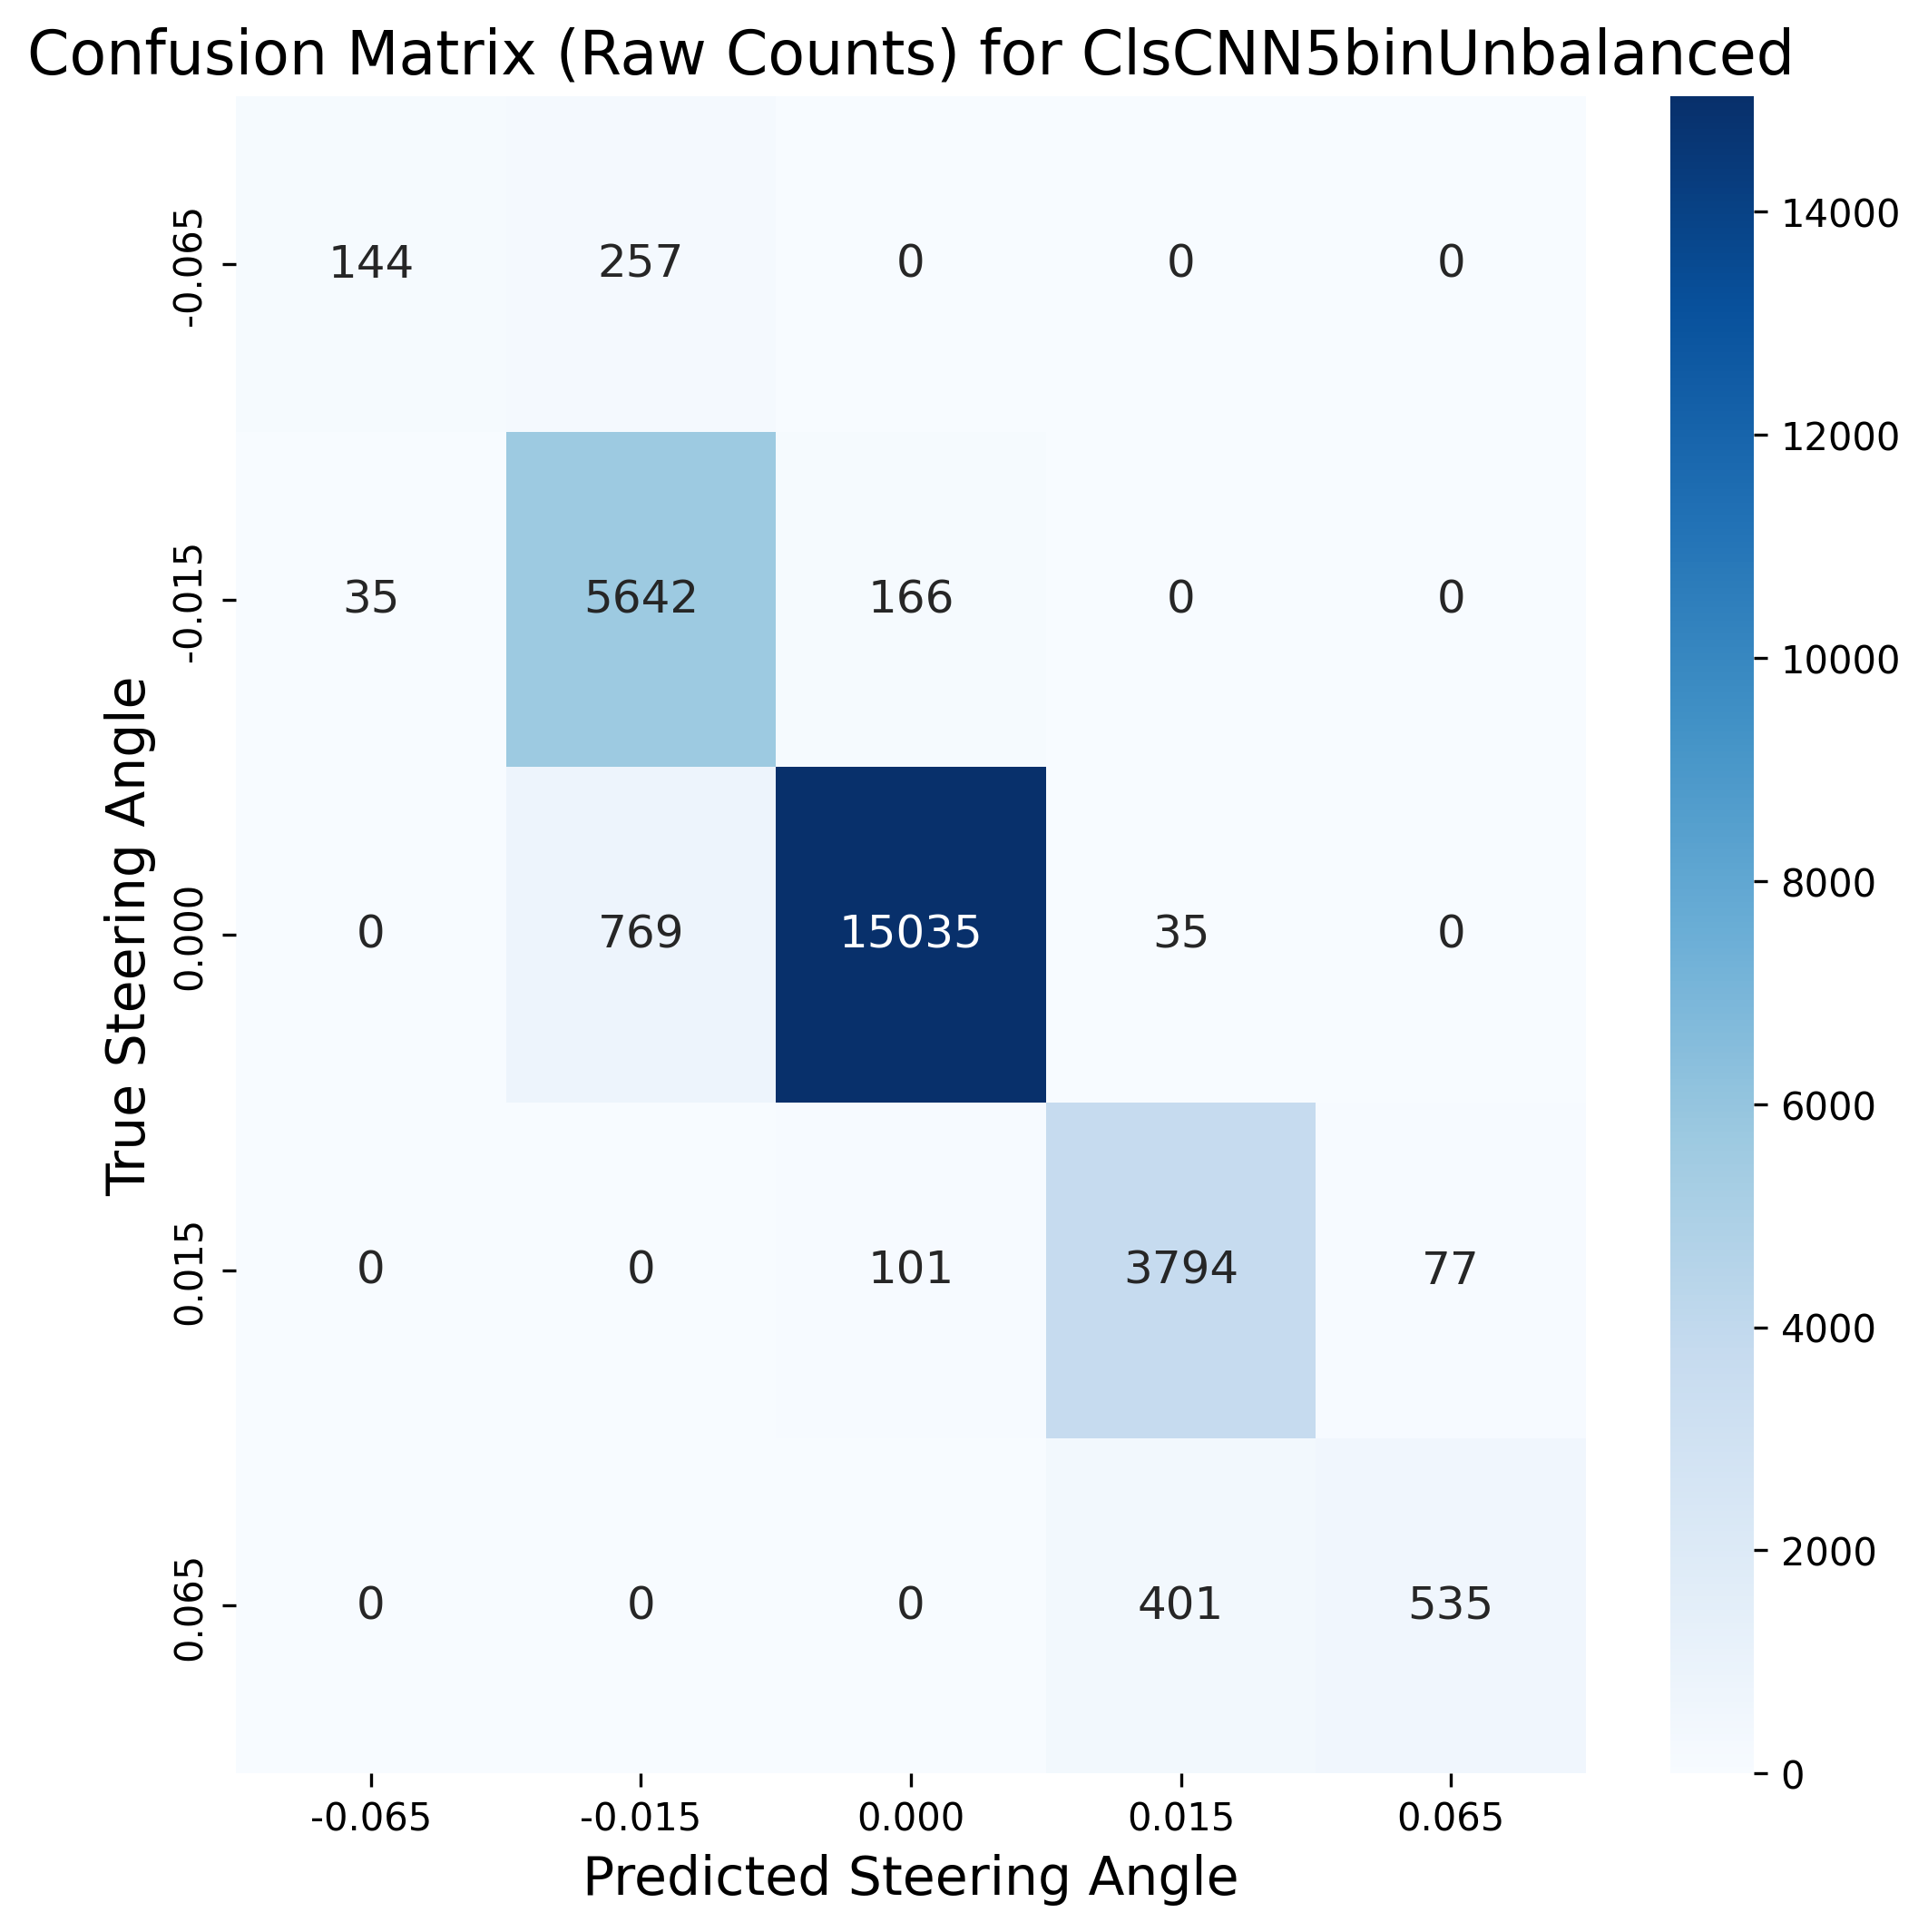
\includegraphics[width=0.65\linewidth]{Figures/Results/cm_raw_ClsCNN5binUnbalanced.png}
\caption{ClsCNN5binUnbalanced model raw counts confusion matrix}
\label{fig:cm_raw_ClsCNN5binUnbalanced}
\end{figure}

\begin{figure}[H]
    \centering
    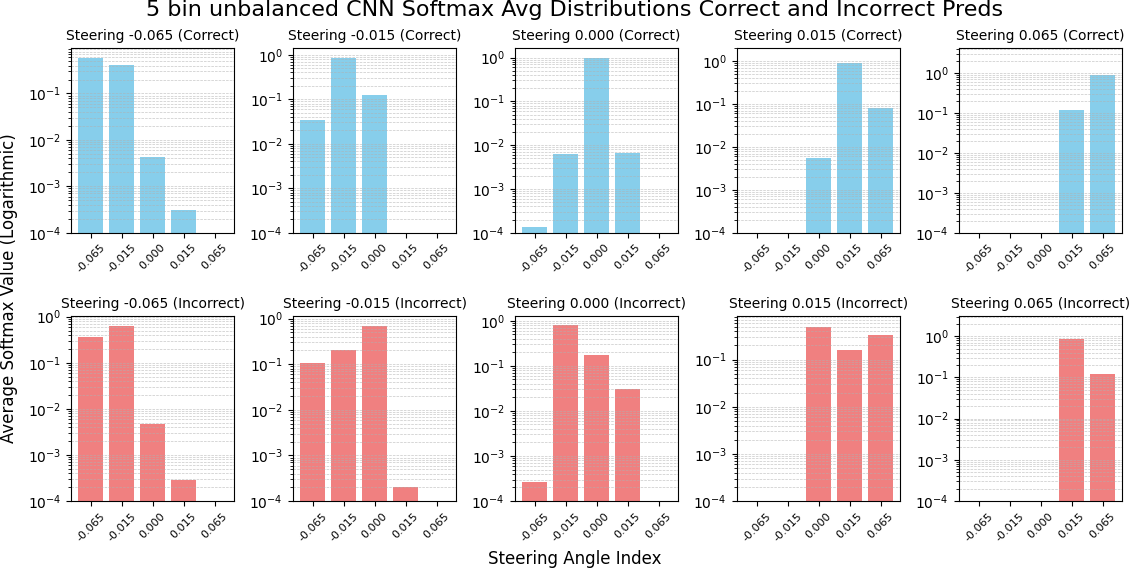
\includegraphics[width=1\linewidth]{Figures/Results/5_bins_cnn_softmax_dist_plot_unbalanced.png}
    \caption{Average softmax Probabilities for Correctly and Incorrectly Classified Steering Angles in the 5 bin cnn unbalanced training Dataset.}
    \label{fig:5_bins_cnn_softmax_dist_unbalanced}
\end{figure}

%%%%%%%%%%%%%%%%%%%%%%
% ClsViT3binBalanced %
%%%%%%%%%%%%%%%%%%%%%%

\textbf{ClsViT3binBalanced}

The ClsViT3binBalanced model was trained using a balanced dataset comprising three discrete steering angle classes corresponding to left, straight, and right maneuvers. Each class contained 22,460 test samples, ensuring uniform class representation during evaluation.

The model achieved an overall classification accuracy of 97.97\% with a mean confidence of 0.9765 across 67,380 test images. Class-wise analysis indicates consistent performance, with precision values between 0.96 and 1.00 and recall values between 0.94 and 1.00. The left and right steering classes ($-0.065$ and $+0.065$) were predicted with near-perfect recall, while the straight class ($0.000$) exhibited a slightly lower recall (0.94), suggesting limited confusion between straight and turning maneuvers.

The macro-averaged precision, recall, and F1-score were each 0.98, confirming balanced performance across classes. These results indicate that the Vision Transformer architecture can effectively capture visual cues relevant to steering direction under a three-bin discretization scheme. The model demonstrates stable behavior in predicting coarse steering categories, supporting its suitability as a perception-based classification component in autonomous driving pipelines.

\begin{table}[htbp]
\centering
\begin{tabular}{@{}lcccc@{}}
\toprule
\textbf{Class} & \textbf{Precision} & \textbf{Recall} & \textbf{F1-Score} & \textbf{Support} \\
\midrule
$-0.065$ & 0.98 & 1.00 & 0.99 & 22,460 \\
$\phantom{-}0.000$ & 1.00 & 0.94 & 0.97 & 22,460 \\
$\phantom{-}0.065$ & 0.96 & 1.00 & 0.98 & 22,460 \\
\midrule
\textbf{Macro Avg} & \textbf{0.98} & \textbf{0.98} & \textbf{0.98} & \textbf{67,380} \\
\bottomrule
\end{tabular}
\caption{Classification performance results for the ClsViT3binBalanced model. The model achieved an overall accuracy of 97.97\% with a mean confidence of 0.9765 across 67,380 test images.}
\label{tab:clf_report_ClsViT3binBalanced}
\end{table}

\begin{figure}[H]
\centering
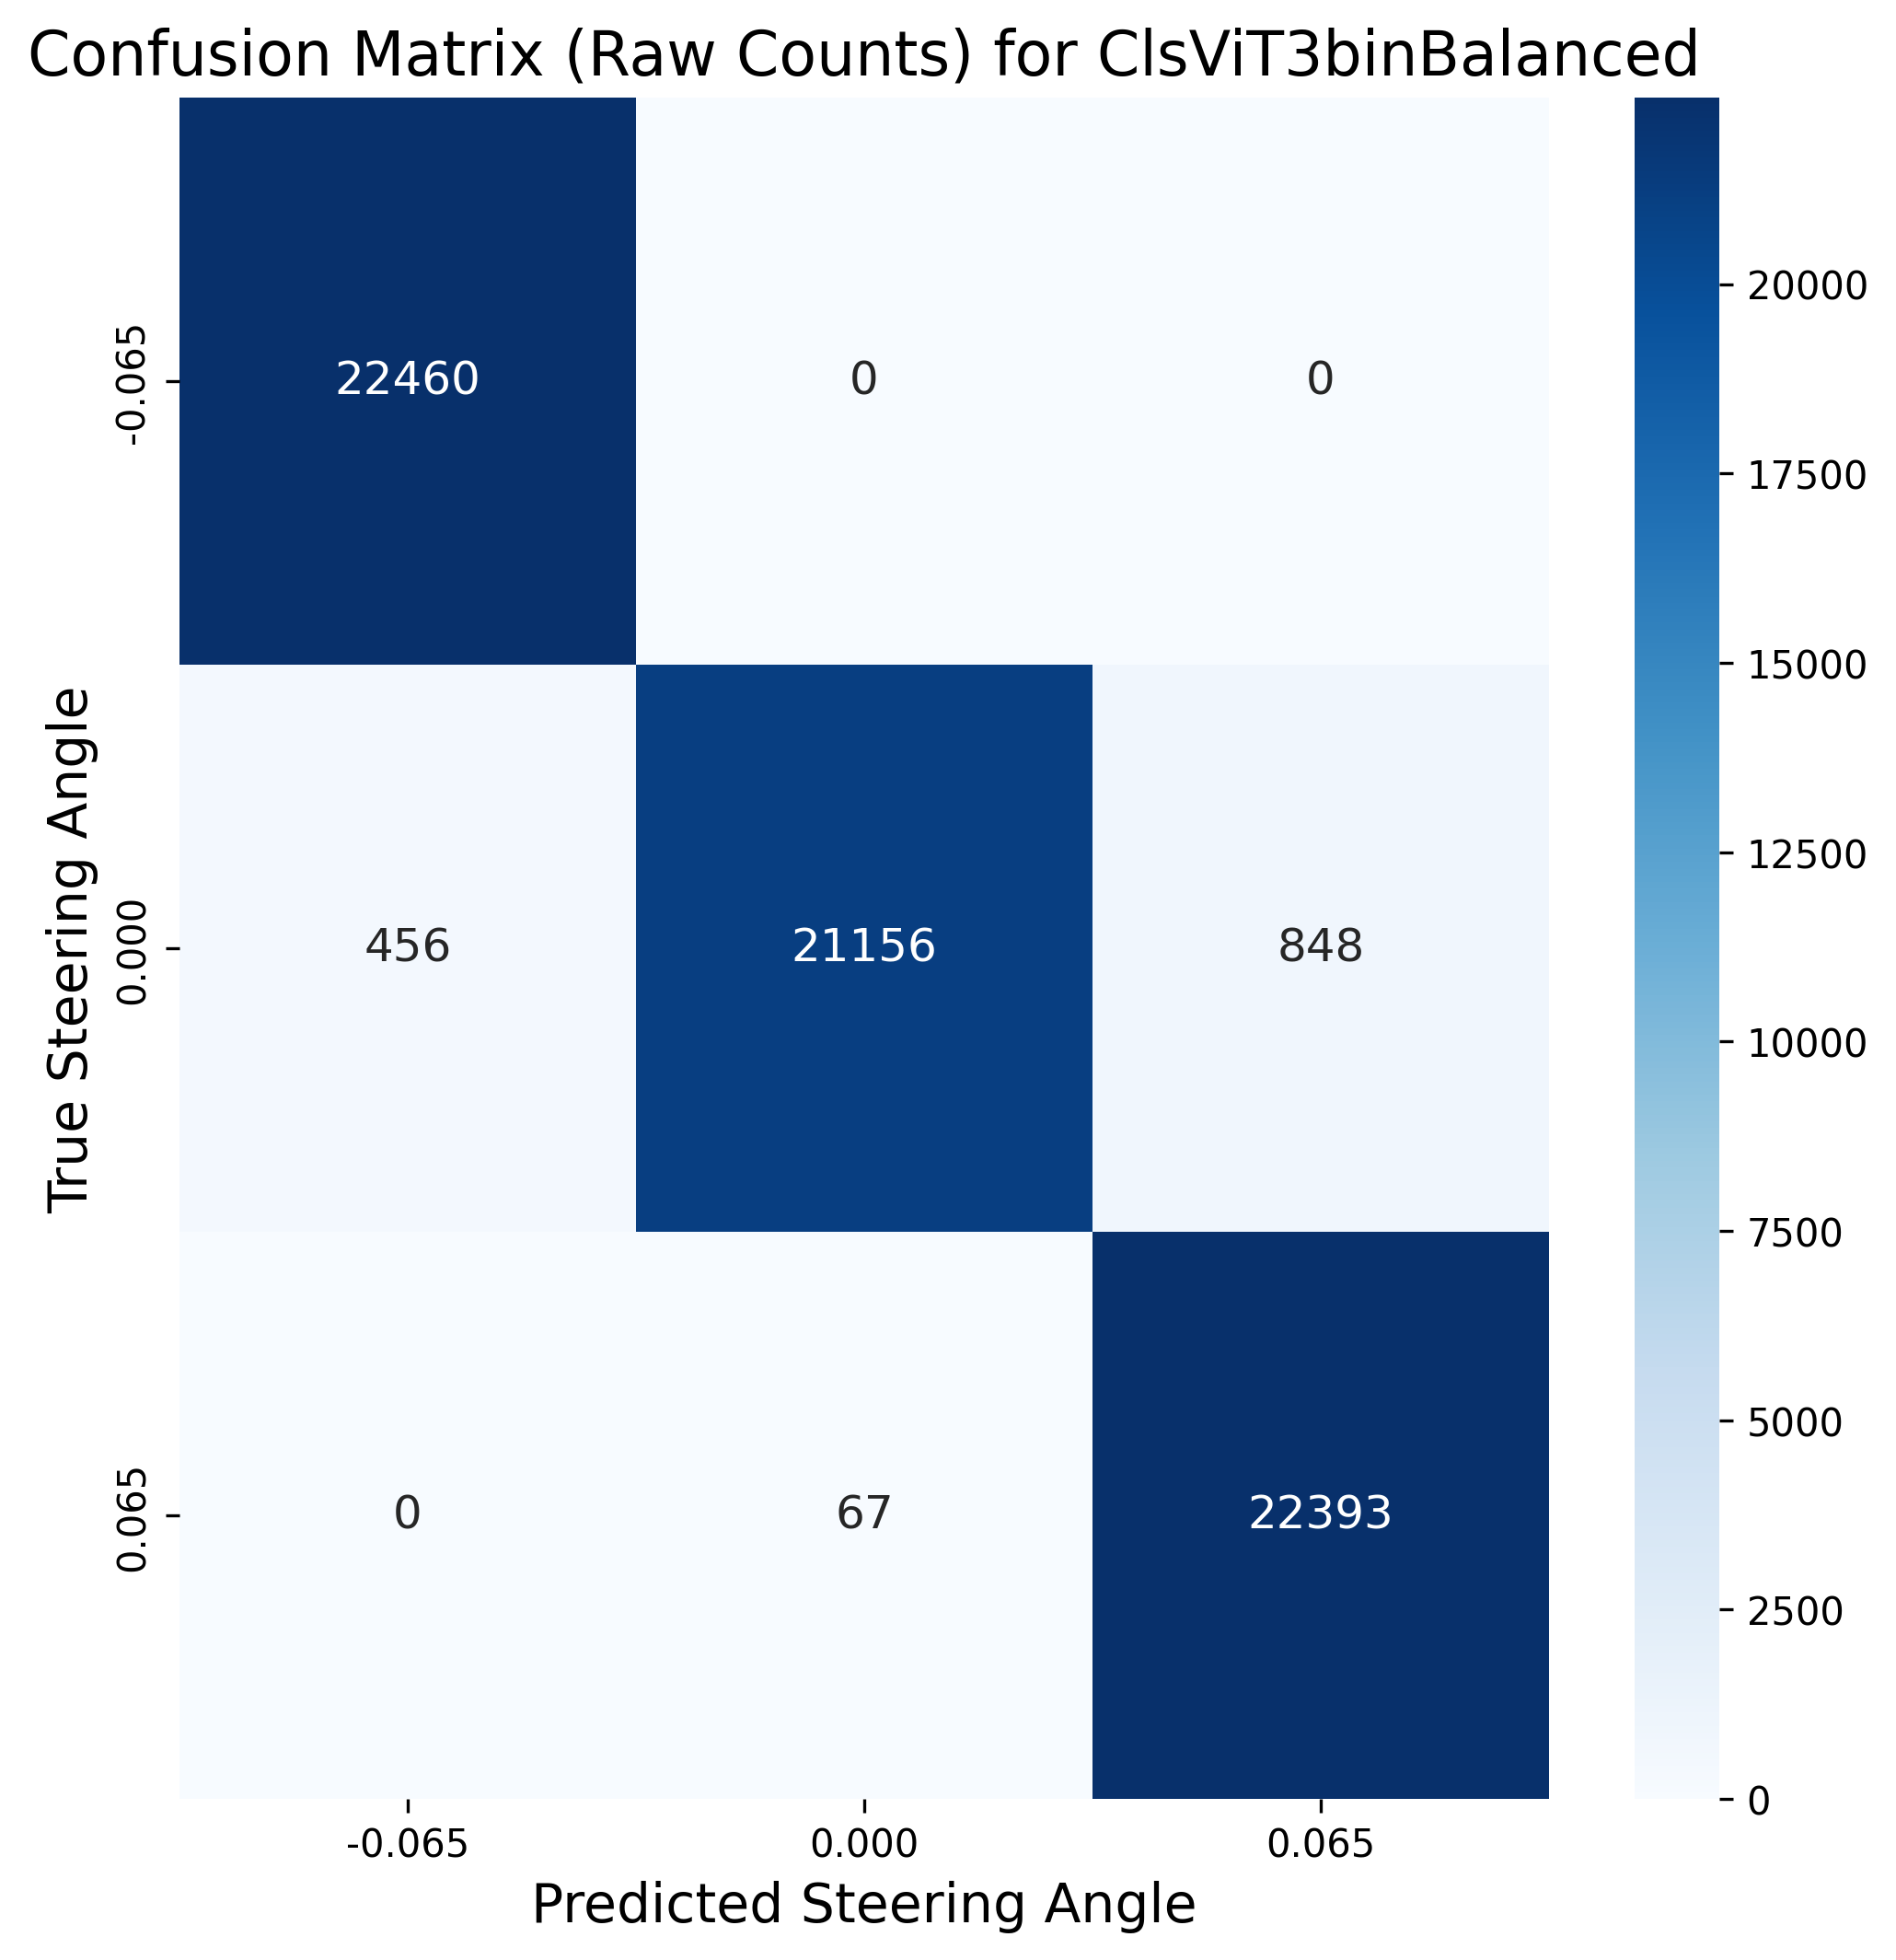
\includegraphics[width=0.65\linewidth]{Figures/Results/cm_raw_ClsViT3binBalanced.png}
\caption{ClsViT3binBalanced model raw counts confusion matrix}
\label{fig:cm_raw_ClsViT3binBalanced}
\end{figure}

\begin{figure}[H]
    \centering
    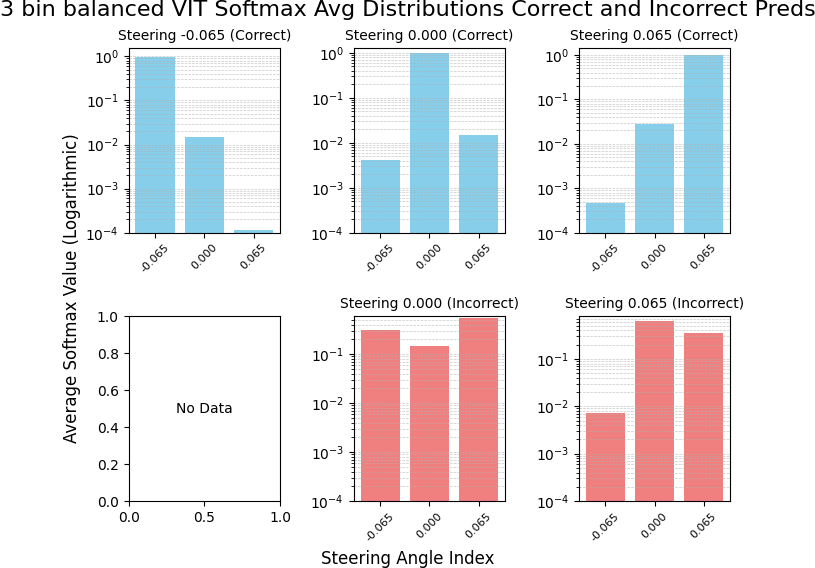
\includegraphics[width=1\linewidth]{Figures/Results/3_bins_vit_softmax_dist_plot_balanced.png}
    \caption{Average softmax Probabilities for Correctly and Incorrectly Classified Steering Angles in the 3 bin vit balanced training Dataset.}
    \label{fig:3_bins_vit_softmax_dist_balanced}
\end{figure}

%%%%%%%%%%%%%%%%%%%%%%
% ClsViT5binBalanced %
%%%%%%%%%%%%%%%%%%%%%%

\textbf{ClsViT5binBalanced}

The ClsViT5binBalanced model was evaluated on a balanced dataset containing five discrete steering angle bins, representing a finer discretization of steering behaviour compared to the three-bin configuration. Each class comprised 15,839 test samples, maintaining equal representation across left, near-left, straight, near-right, and right steering categories.

The model achieved an overall accuracy of 97.77\% with a mean confidence of 0.9779 across 79,195 test images. Performance across all classes was consistent, with precision and recall values ranging between 0.95 and 1.00. The outermost bins ($\pm0.065$) achieved perfect or near-perfect recall, while intermediate bins ($\pm0.015$) and the straight class ($0.000$) showed slightly lower recall (0.95–0.99). These results indicate that the Vision Transformer maintains stable predictive performance even under finer steering quantization, without significant degradation across bins.

The macro-averaged precision, recall, and F1-score were each 0.98, confirming uniform classification performance across all steering directions. Overall, the results demonstrate that the ViT architecture generalizes effectively under balanced training conditions, capturing spatial and contextual dependencies relevant to steering classification in the five-bin discretization framework.

\begin{table}[htbp]
\centering
\begin{tabular}{@{}lcccc@{}}
\toprule
\textbf{Class} & \textbf{Precision} & \textbf{Recall} & \textbf{F1-Score} & \textbf{Support} \\
\midrule
$-0.065$ & 0.99 & 1.00 & 1.00 & 15,839 \\
$-0.015$ & 0.96 & 0.99 & 0.97 & 15,839 \\
$\phantom{-}0.000$ & 0.99 & 0.95 & 0.97 & 15,839 \\
$\phantom{-}0.015$ & 1.00 & 0.95 & 0.97 & 15,839 \\
$\phantom{-}0.065$ & 0.96 & 1.00 & 0.98 & 15,839 \\
\midrule
\textbf{Macro Avg} & \textbf{0.98} & \textbf{0.98} & \textbf{0.98} & \textbf{79,195} \\
\bottomrule
\end{tabular}
\caption{Classification performance results for the ClsViT5binBalanced model. The model achieved an overall accuracy of 97.77\% with a mean confidence of 0.9779 across 79,195 test images.}
\label{tab:clf_report_ClsViT5binBalanced}
\end{table}

\begin{figure}[H]
\centering
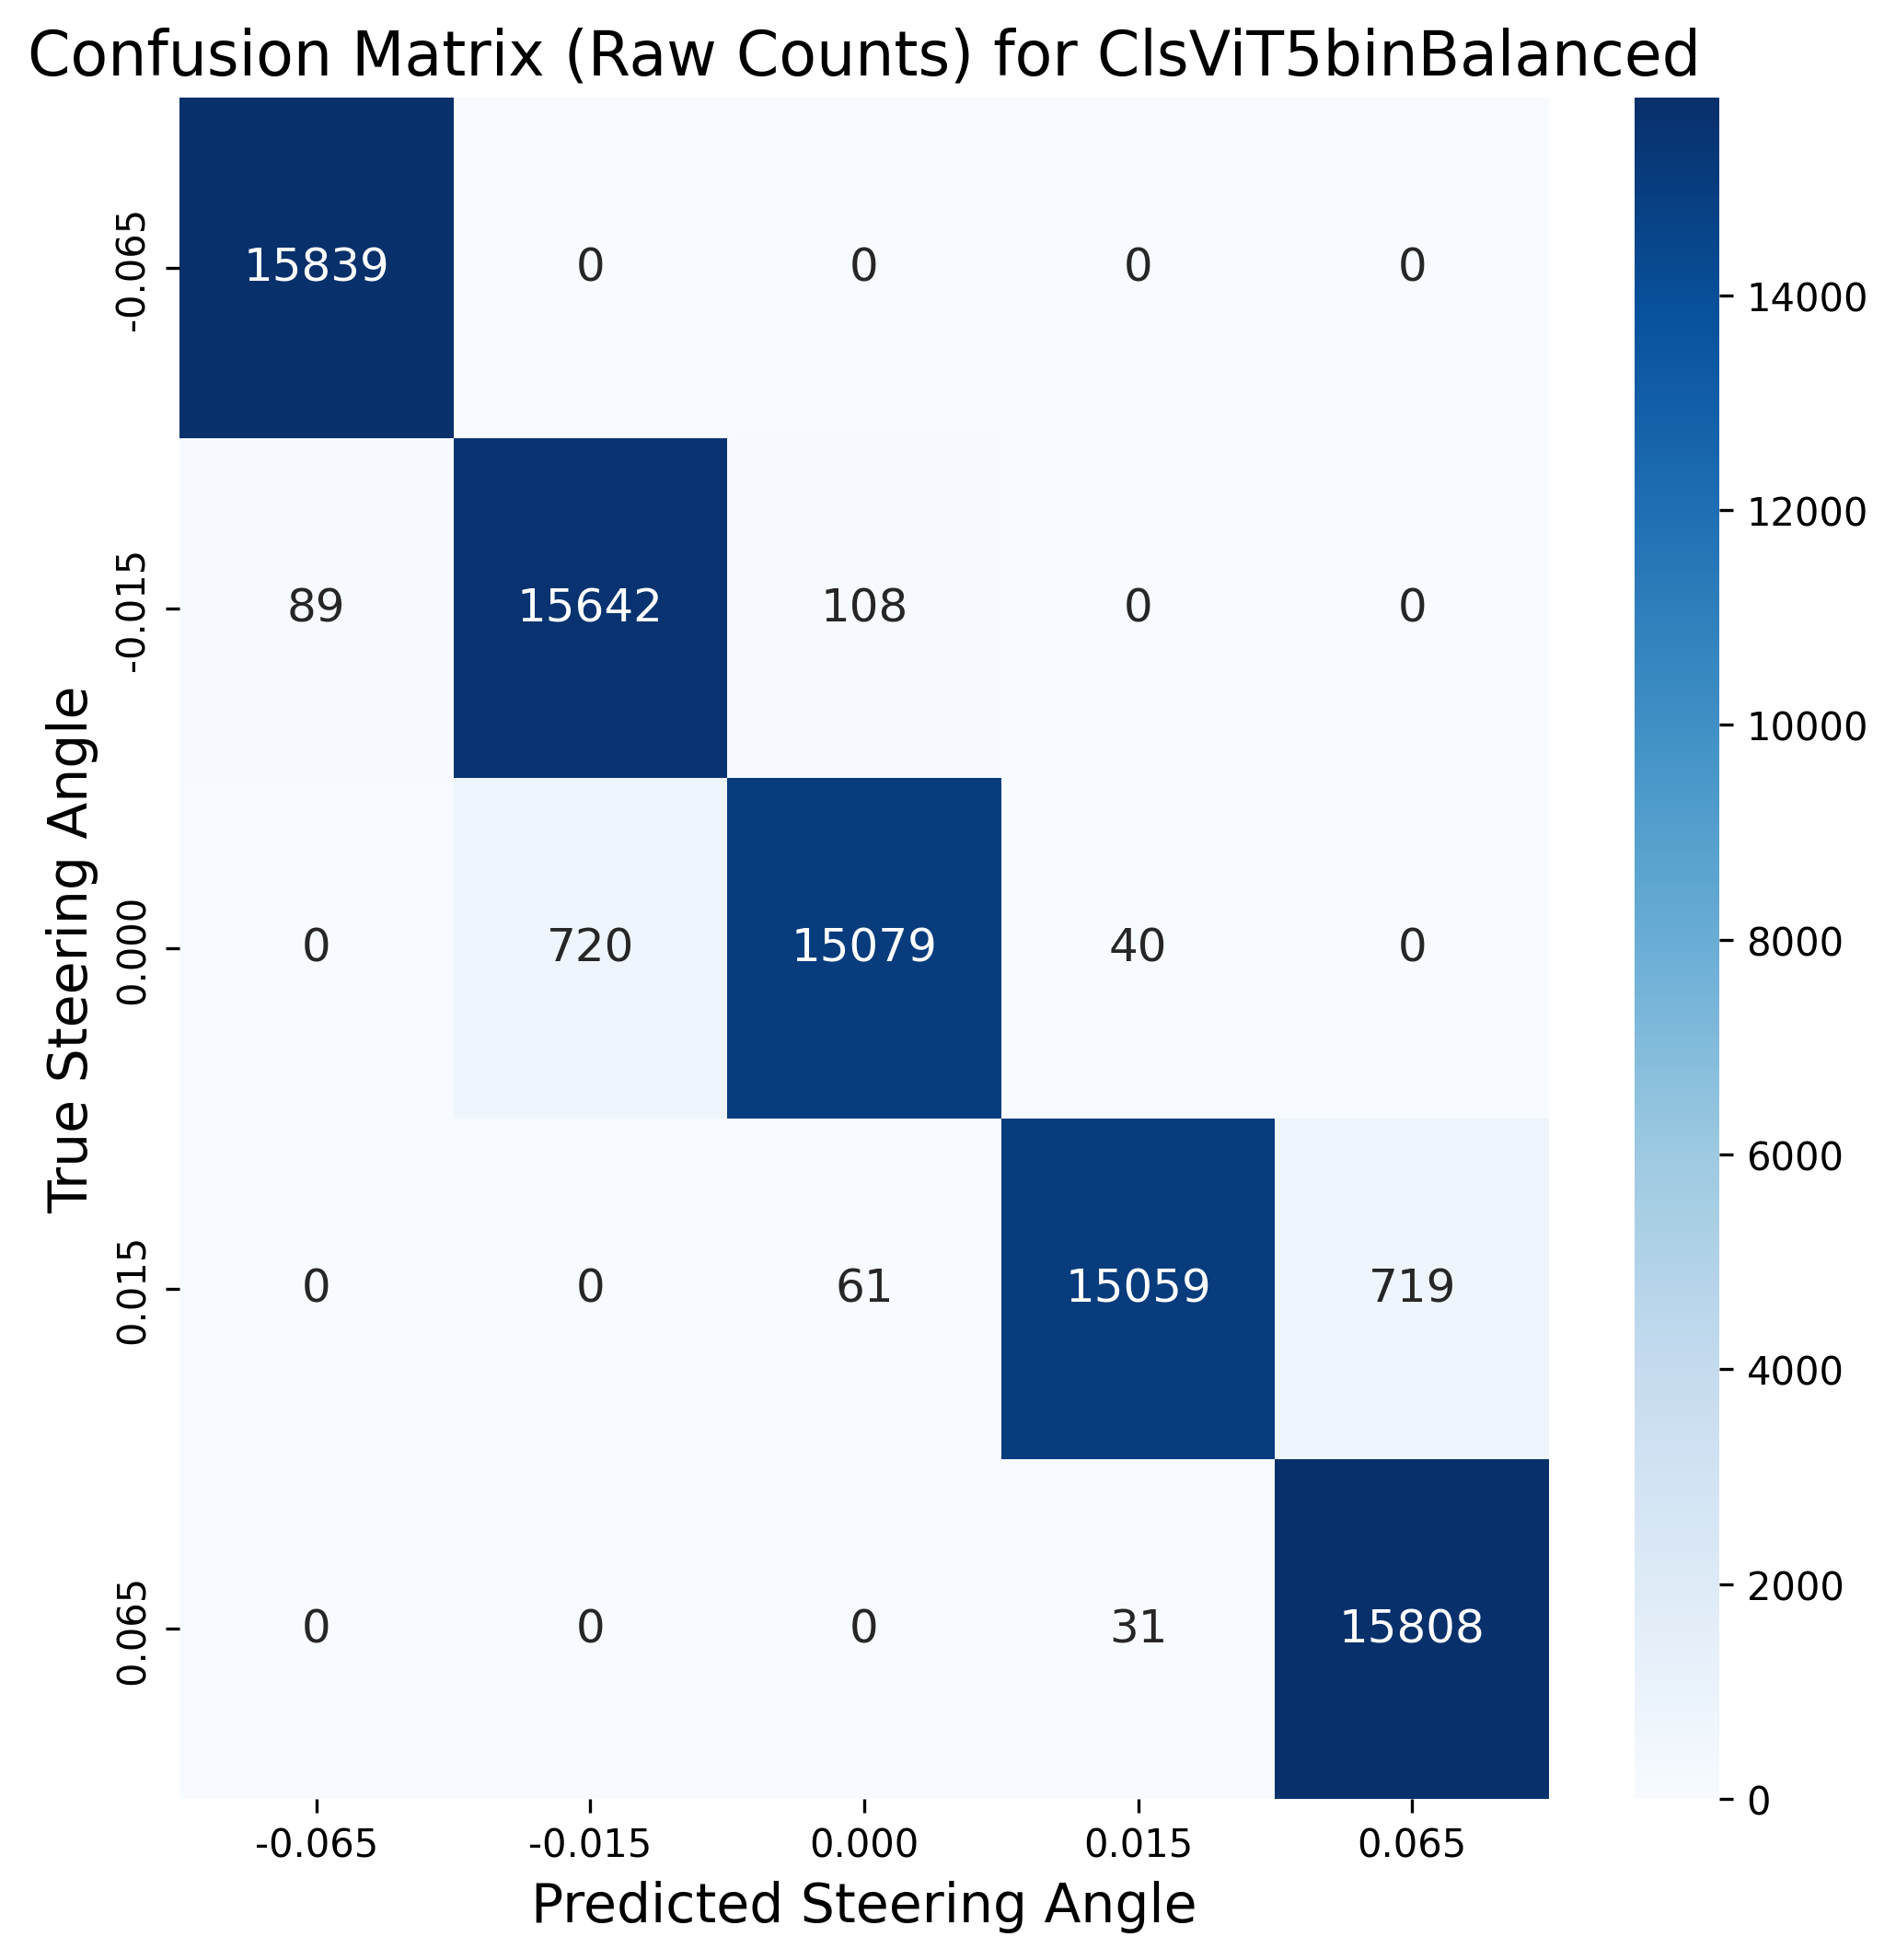
\includegraphics[width=0.65\linewidth]{Figures/Results/cm_raw_ClsViT5binBalanced.png}
\caption{ClsViT5binBalanced model raw counts confusion matrix}
\label{fig:cm_raw_ClsViT5binBalanced}
\end{figure}

\begin{figure}[H]
    \centering
    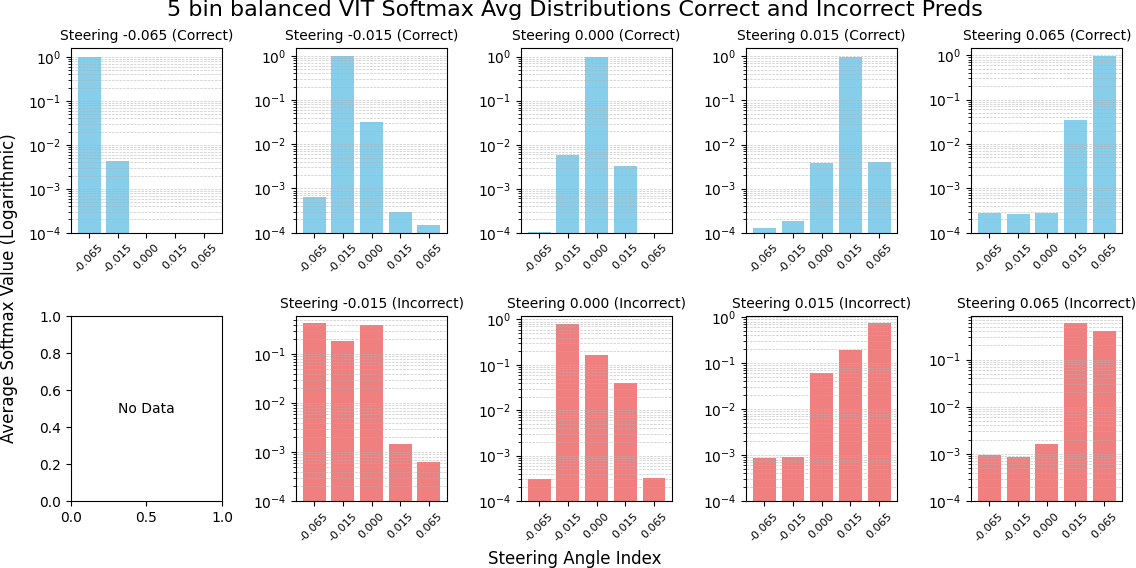
\includegraphics[width=1\linewidth]{Figures/Results/5_bins_vit_softmax_dist_plot_balanced.png}
    \caption{Average softmax Probabilities for Correctly and Incorrectly Classified Steering Angles in the 5 bin vit balanced training Dataset.}
    \label{fig:5_bins_vit_softmax_dist_balanced}
\end{figure}

%%%%%%%%%%%%%%%%%%%%%%%%%%%%%%%%%%%%%%
% NOISE IN SELF-DRIVING APPLICATIONS %
%%%%%%%%%%%%%%%%%%%%%%%%%%%%%%%%%%%%%%

\section{Classifier Models in Self-Driving Applications}

Channel-wise salt-and-pepper noise is applied to the RGB image by first calculating the noise probability $p = \text{intensity} \times 0.01$, then generating a three-dimensional boolean mask $M$ with the same shape as the RGB image where each element $M_{i,j,k}$ (for pixel $(i,j)$ and colour channel $k \in \{R,G,B\}$) is set to True with probability $p$. The mask is then applied to a copy of the original RGB image where each True element in the mask corresponds to a colour channel that gets corrupted: the original channel value $I_{i,j,k}$ is replaced with a new value $I'_{i,j,k} = \text{random}(0,1) \times 255$, which results in either 0 or 255. Since each of the three RGB channels is independently corrupted, a single pixel can exhibit any of the eight possible colour combinations shown in Table \ref{tab:channel_wise_salt_pepper_colors}, ranging from pure black (when all channels are set to 0) to pure white (when all channels are set to 255), with intermediate colours like red, green, blue, cyan, magenta, and yellow when channels are mixed.

\begin{longtable}{@{}llll@{}}
\toprule
R & G & B & Resulting Colour \\
\midrule
\endfirsthead
\toprule
R & G & B & Resulting Colour \\
\midrule
\endhead
0 & 0 & 0 & Black \\
0 & 0 & 255 & Blue \\
0 & 255 & 0 & Green \\
0 & 255 & 255 & Cyan \\
255 & 0 & 0 & Red \\
255 & 0 & 255 & Magenta \\
255 & 255 & 0 & Yellow \\
255 & 255 & 255 & White \\
\bottomrule
\caption{Possible pixel values and colours when channel-wise salt-and-pepper noise is applied independently to RGB channels}
\label{tab:channel_wise_salt_pepper_colors}
\end{longtable}




%%%%%%%%%%%%%%%%%%%%%%%%%%%%%%%%%%%%%%%%%%%%%%%%%%%
% FIGURE - COMBINED 3%, 10%, 50% NOISE APPLIED TO %
% VEHICLE CAMERA                                  %
%%%%%%%%%%%%%%%%%%%%%%%%%%%%%%%%%%%%%%%%%%%%%%%%%%%

\begin{figure}[H]
    \centering
    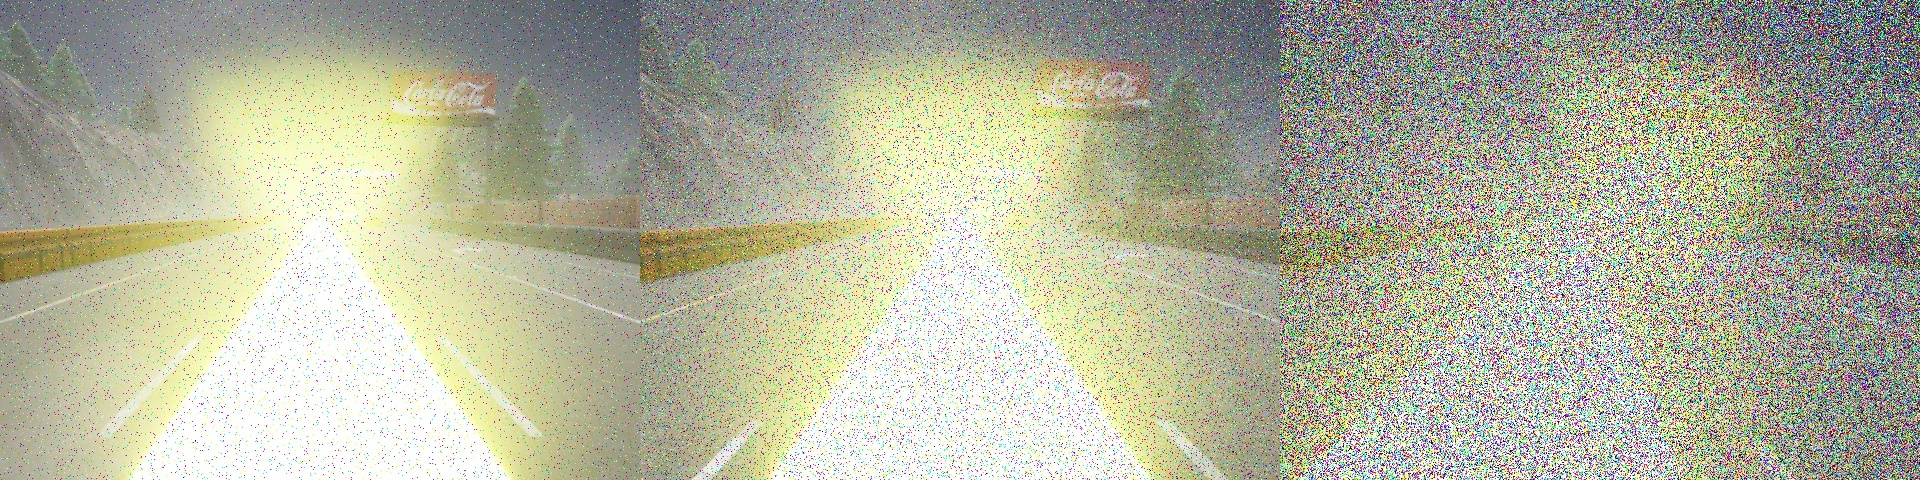
\includegraphics[width=1.0\linewidth]{Figures/Results/experiment-247-251-255-3pc-10pc-50pc-rbg-pepper-noise-combined.jpg}
    \caption{CARLA simulator vehicle camera RGB image with 3\% (left), 10\% (middle) and 50\% channel-wise salt-and-pepper noise applied}
    \label{fig:experiment-247-251-255-3pc-10pc-50pc-rbg-pepper-noise-combined}
\end{figure}

Figure \ref{fig:experiment-247-251-255-3pc-10pc-50pc-rbg-pepper-noise-combined} shows images as would be presented to CNN (before preprocessing) and ViT networks (as is) for steering prediction. The image is generated by starting the simulation and saving one image. The images with channel-wise salt-and-pepper noise shown in the figure, were generated from left to right by experiments 247, 251 and 255.

\textbf{Self-driving softmax Output Analysis}

%%%%%%%%%%%%%%%%%%%%%%%%%%%%%%%%%%%%%%%%%%%%
% FIGURES NOISE METRICS WITH LANE INVASION %
%%%%%%%%%%%%%%%%%%%%%%%%%%%%%%%%%%%%%%%%%%%%


% figures generated by experiment 268




%%%%%%%%%%%%%%%%%%%%%%%%%%%%%%%%%%%%%%%%%%%%%%
% COMBINED DISTANCE METRICS - EXPERIMENT 268 %
%%%%%%%%%%%%%%%%%%%%%%%%%%%%%%%%%%%%%%%%%%%%%%

% NB Experiment 268 aggregates values from 
\begin{figure}[H]
    \centering
    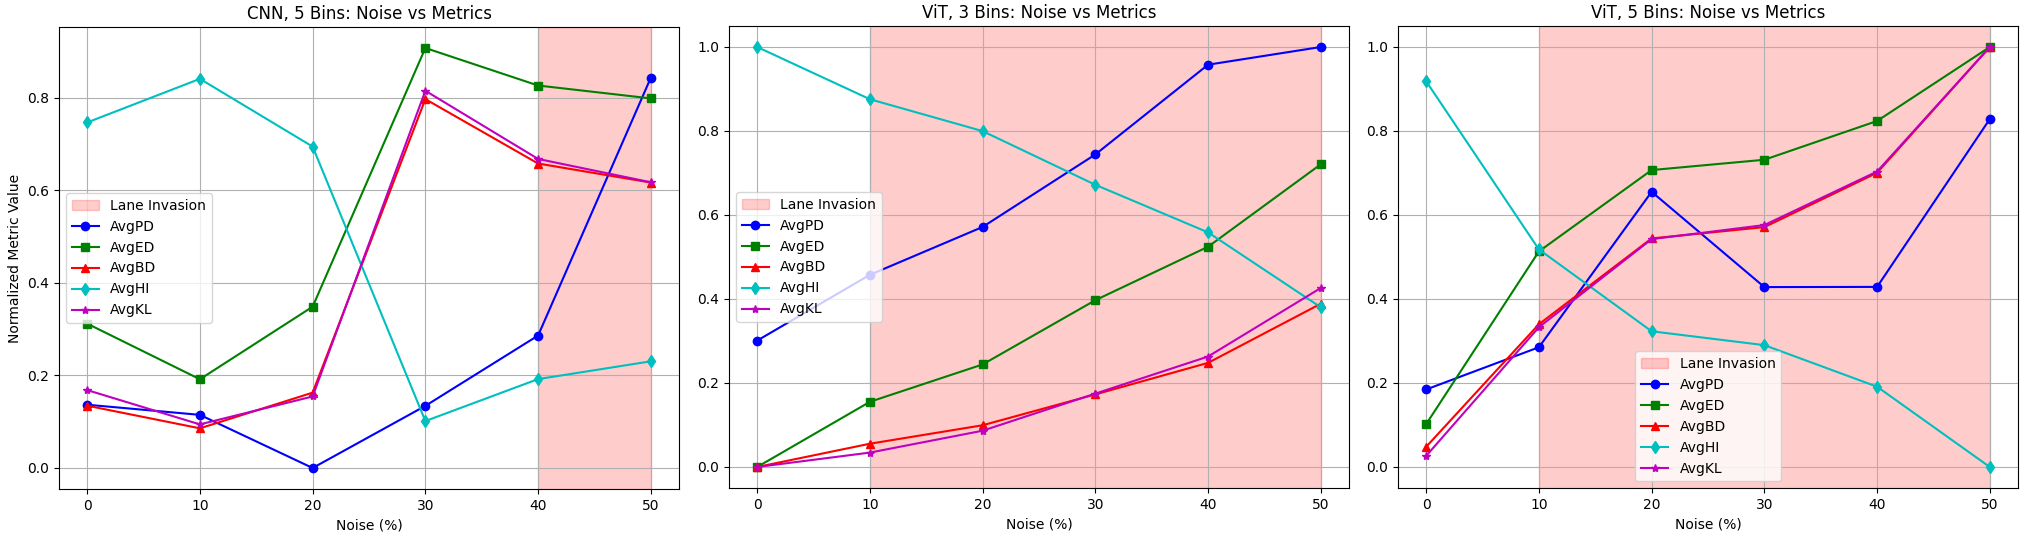
\includegraphics[width=1.0\linewidth]{Figures/Results/combined_cnn_5bin_vit_3bin_vit_5bin_noise_distance_metrics.png}
    \caption{Combined CNN 5 bin (left), ViT 3 bin (middle) and ViT 5 bin (right) noise levels by Average Path Distance (blue), Average Euclidean Distance (green), Average Bhattacharyya Distance (red), Average Histogram Intersection (cyan) and Average KL Divergence (purple). The pink band indicates noise levels where lane invasions occurred}
    \label{fig:combined_cnn_5bin_vit_3bin_vit_5bin_noise_distance_metrics}
\end{figure}

Figure \ref{fig:combined_cnn_5bin_vit_3bin_vit_5bin_noise_distance_metrics}, shows the general trend that as noise levels increase, all distance metrics also increase, except Histogram Intersection, which has a maximum value of 1 when images all RGB pixels are identical (0\% noise), and decreases as noise is added, original and noisy image becoming dissimilar.
To obtain one data point in the plot, pepper noise is applied to the RGB image at 0, 10, 20, 30, 40 and 50\% pixel ratios. An average is taken for all predicted softmax output Euclidean distances to centroids, across all classes (AvgED). An average distance is taken from the vehicle to the lane path across all path distance readings acquired during the simulation (AvgPD). The following averages are taken between the original image and the noisy image for all images generated by the simulation: Bhattacharyya Distance (AvgBD), Histogram Intersection (AvgHI), KL Divergence (AvgKL). Min-max normalization was applied to the averages being plotted, following the formula $x_{norm} = (x - x_{min}) / (x_{max} - x_{min})$, which scales all values to the range [0,1].

Bhattacharyya Distance, Histogram Intersection and KL Divergence cannot be quantified in real world conditions because, unlike simulated scenarios, there is no "reference" image to be compared with. The metrics are still useful to confirm there exists a level of separation between the captured image and the image presented to the network, given noise. Distance to path cannot be quantified in real world conditions because the simulated path is determined by objects (waypoints) generated by the simulation, which exist as transform objects in simulation but not in the real world. The key metric, determining if the model is "outside of its comfort zone", is the Average Euclidean Distance. The Euclidean distance between the network's softmax output and the pre-computed class (discretized steering angles) centroids is the only quantity that can be computed in the wild.
The pink region of the plots mark the occurrence of lane invasions. For example, the left hand side plot for the CNN trained on 5 bin quantized (-0.065, -0.015, 0.0000, 0.0150 and 0.0650 steering angle classes) balanced data: , presented lane invasions where at 40\% noise, where 40\% noise would approximately correspond to the right hand side image in Figure \ref{fig:combined_cnn_5bin_vit_3bin_vit_5bin_noise_distance_metrics}. 

Table \ref{tab:experiment_stats_common_0_10_20_30_40_50} presents results for experiments that were common to the three models tested - the best performing CNN model (5 bin-quantized unbalanced-dataset, 93.18\% overall accuracy) the corresponding best performing 5 bin-quantized balanced-dataset ViT model (97.77\% overall accuracy) and the best performing model overall, the ViT 3 bin-quantized balanced-dataset model (97.97\% overall accuracy).

Further, Table \ref{tab:experiment_stats_common_0_10_20_30_40_50} presents the original values used to compute the plots in Figure \ref{fig:combined_cnn_5bin_vit_3bin_vit_5bin_noise_distance_metrics}. The bold font in consecutive rows, column AvgED, shows where a lane invasion was observed. For example, in experiment 240, the CNN 5 bin model steering, with front facing camera images subject to 40\% noise, lead to a lane invasion (column LI presenting value T). The lane invasion lead to the simulation being stopped at frame count 10133 (FrCnt). The average distance to the optimal trajectory path (AvrPD) was recorded at 0.1080 units of distance for the all distance to path readings (PDCont), the average Euclidean distance to predicted class centroid (AvgED) was recorded at 0.6257 (across all predictions, corresponding in number to the frame count FrCnt). In general the average Bhattacharya Distance (AvgBD) and KL Divergence (AvgKL) tend to increase with noise, while Histogram Intersection (AvgHI) tends to decrease with noise.
The average Euclidean distance to the predicted class centroid (AvgED) tend to increase with noise. 
Since the aim is to ensure autonomous system safety, a prediction, under the experimental parameters, can be considered safe when no lane invasion occurs. Therefore, we make note of the nearest average Euclidean distance to predicted class centroid, where a lane invasion occurred while the simulated vehicle was steering with predictions from the CNN 5 bin classifier. The nearest average (lowest value) was observed in experiment 241, 0.6061. We note that there are higher averages - experiment 239, 30\% noise, 0.6828 - where lane invasions did not occur. Our choice for threshold for the CNN 5 bin model should be between 0.6061 and 0.2829 average Euclidean distance from the class softmax outputs to the predicted class centroids. In other words, the threshold should be placed between the highest AvgED value where a lane invasion did not occur and the lowest AvgED value where a lane invasion occurred, for a given model. We highlight the values in boldface in Table \ref{tab:experiment_stats_common_0_10_20_30_40_50}. In short, for the CNN 5 bin classifier, the threshold should be placed between 0.2892 and 0.6061. 

Based on the common results, for noise levels 0, 10, 20, 30, 40 and 50\%, and applying the same constraints, the ViT 3 bin threshold should be placed between 0.0437 and 0.1530. In practice, the ViT 3 bin model presented lane invasions at lower noise levels compared to the CNN 5 bin model, leading to shorter intervals. 
We present the full results in Table \ref{tab:experiment_stats}.

%%%%%%%%%%%%%%%%%%%%%%%%%%%%%%%%%%%%%%%%%%%%%%%%%%%%
% COMMON RESULTS TABLE (0,10,20,30,40,50pct noise) %
%%%%%%%%%%%%%%%%%%%%%%%%%%%%%%%%%%%%%%%%%%%%%%%%%%%%

\begin{longtable}{@{}cllrrrrrrrrrc@{}}
\toprule
Exp & Net & Bins & Noise & AvgPD & PDCnt & AvgED & AvgBD & AvgHI & AvgKL & FrCnt & LI \\
\midrule
\endfirsthead
\toprule
Exp & Net & Bins & Noise & AvgPD & PDCnt & AvgED & AvgBD & AvgHI & AvgKL & FrCnt & LI \\
\midrule
\endhead
262 & CNN & 5 & 0 & 0.0600 & 1032 & 0.2634 & 0.0706 & 0.8091 & 0.1016 & 19749 & F \\
237 & CNN & 5 & 10 & 0.0529 & 1032 & 0.1787 & 0.0493 & 0.8681 & 0.0699 & 20534 & F \\
238 & CNN & 5 & 20 & 0.0160 & 1032 & \textbf{0.2892} & 0.0829 & 0.7765 & 0.0957 & 22356 & F \\
239 & CNN & 5 & 30 & 0.0592 & 1032 & 0.6828 & 0.3588 & 0.4053 & 0.3785 & 22375 & F \\
240 & CNN & 5 & 40 & 0.1080 & 473 & 0.6257 & 0.2982 & 0.4621 & 0.3154 & 10133 & T \\
241 & CNN & 5 & 50 & 0.2871 & 473 & \textbf{0.6061} & 0.2803 & 0.4861 & 0.2938 & 10550 & T \\
263 & ViT & 3 & 0 & 0.1127 & 1032 & \textbf{0.0437} & 0.0120 & 0.9676 & 0.0296 & 8736 & F \\
251 & ViT & 3 & 10 & 0.1631 & 17 & \textbf{0.1530} & 0.0362 & 0.8898 & 0.0443 & 130 & T \\
252 & ViT & 3 & 20 & 0.1997 & 15 & 0.2156 & 0.0553 & 0.8423 & 0.0666 & 108 & T \\
253 & ViT & 3 & 30 & 0.2552 & 12 & 0.3234 & 0.0872 & 0.7623 & 0.1044 & 90 & T \\
254 & ViT & 3 & 40 & 0.3238 & 8 & 0.4130 & 0.1199 & 0.6914 & 0.1422 & 58 & T \\
255 & ViT & 3 & 50 & 0.3374 & 5 & 0.5513 & 0.1811 & 0.5798 & 0.2120 & 34 & T \\
266 & ViT & 5 & 0 & 0.0753 & 1032 & \textbf{0.1156} & 0.0330 & 0.9165 & 0.0409 & 4358 & F \\
256 & ViT & 5 & 10 & 0.1076 & 39 & \textbf{0.4051} & 0.1599 & 0.6660 & 0.1720 & 164 & T \\
257 & ViT & 5 & 20 & 0.2266 & 25 & 0.5415 & 0.2488 & 0.5440 & 0.2618 & 101 & T \\
258 & ViT & 5 & 30 & 0.1537 & 30 & 0.5588 & 0.2605 & 0.5234 & 0.2761 & 120 & T \\
259 & ViT & 5 & 40 & 0.1538 & 40 & 0.6238 & 0.3167 & 0.4615 & 0.3307 & 157 & T \\
260 & ViT & 5 & 50 & 0.2823 & 29 & 0.7479 & 0.4470 & 0.3418 & 0.4576 & 114 & T \\
\bottomrule
\caption{Common experiment results for noise levels 0\%, 10\%, 20\%, 30\%, 40\%, and 50\% across three models: CNN 5-bin (unbalanced dataset, 93.18\% accuracy), ViT 5-bin (balanced dataset, 97.77\% accuracy), and ViT 3-bin (balanced dataset, 97.97\% accuracy). The table reports metrics including average path deviation (AvgPD), path deviation count (PDCnt) - this is the number of times in the simulation the distance from the vehicle from the path was computed, average Euclidean distance to predicted class centroid (AvgED, bolded where lane invasions occurred), average Bhattacharyya distance (AvgBD), average histogram intersection (AvgHI), average KL divergence (AvgKL), frame count (FrCnt), and lane invasion status (LI, T for true, F for false). These metrics underpin the plots in Figure~\ref{fig:combined_cnn_5bin_vit_3bin_vit_5bin_noise_distance_metrics}. For safety, thresholds for AvgED are proposed to avoid lane invasions: for CNN 5-bin, between 0.2892 (highest safe) and 0.6061 (lowest unsafe); for ViT 3-bin, between 0.0437 and 0.1530; for ViT 5-bin, between 0.1156 and 0.4051.}
\label{tab:experiment_stats_common_0_10_20_30_40_50}
\end{longtable}

% Removed, cannot find this table
% Full results are in Appendix~\ref{AppendixG-full-results}, Table~\ref{tab:experiment_stats_full_0_10_20_30_40_50}.}

% LOD Paper Integration - Theoretical Foundation for Threshold-Based Safety
\textbf{Setting Distance-to-Centroid Thresholds}

The threshold selection methodology for preventing lane invasions applies framework described in the contributions, which demonstrates that Euclidean distance between softmax outputs and class centroids serves as a proxy for prediction confidence. The work establishes that setting distance thresholds based on distances from incorrect predictions to class centroids enables systems to identify unreliable predictions and defer judgment.

In our autonomous driving implementation, this translates to safety thresholds: when steering predictions exceed the distance threshold to their class centroid, the system should reject the prediction as potentially unsafe. The threshold ranges in Table \ref{tab:experiment_stats_common_0_10_20_30_40_50} represent conservative boundaries derived from the minimum distance observed for lane invasions in our simulated scenarios. 

%%%%%%%%%%%%%%%%%%%%%%
% MAIN RESULTS TABLE %
%%%%%%%%%%%%%%%%%%%%%%

% The main thing shown here is that for ViT models lane invasions start with **minimal**
% noise. That can also be stated in the condensed table (to match noise levels for all
% models).

% NOTE: Full results table commented out - move to appendix if needed
% \begin{longtable}{@{}cllrrrrrrrrrc@{}}
% \toprule
% Exp & Net & Bins & Noise & AvgPD & PDCnt & AvgED & AvgBD & AvgHI & AvgKL & FrCnt & LI \\
% \midrule
% \endfirsthead
% \toprule
% Exp & Net & Bins & Noise & AvgPD & PDCnt & AvgED & AvgBD & AvgHI & AvgKL & FrCnt & LI \\
% \midrule
% \endhead
% 262 & CNN & 5 & 0 & 0.0600 & 1032 & 0.2634 & 0.0706 & 0.8091 & 0.1016 & 19749 & F \\
% 237 & CNN & 5 & 10 & 0.0529 & 1032 & 0.1787 & 0.0493 & 0.8681 & 0.0699 & 20534 & F \\
% 238 & CNN & 5 & 20 & 0.0160 & 1032 & 0.2892 & 0.0829 & 0.7765 & 0.0957 & 22356 & F \\
% 239 & CNN & 5 & 30 & 0.0592 & 1032 & 0.6828 & 0.3588 & 0.4053 & 0.3785 & 22375 & F \\
% 240 & CNN & 5 & 40 & 0.1080 & 473 & 0.6257 & 0.2982 & 0.4621 & 0.3154 & 10133 & T \\
% 241 & CNN & 5 & 50 & 0.2871 & 473 & 0.6061 & 0.2803 & 0.4861 & 0.2938 & 10550 & T \\
% 242 & CNN & 5 & 55 & 0.3853 & 189 & 0.5933 & 0.2715 & 0.5011 & 0.2823 & 4146 & T \\
% 243 & CNN & 5 & 60 & 0.3105 & 18 & 0.5292 & 0.2141 & 0.5533 & 0.2342 & 369 & T \\
% 263 & ViT & 3 & 0 & 0.1127 & 1032 & 0.0437 & 0.0120 & 0.9676 & 0.0296 & 8736 & F \\
% 245 & ViT & 3 & 1 & 0.1805 & 217 & 0.1063 & 0.0255 & 0.9232 & 0.0339 & 930 & T \\
% 246 & ViT & 3 & 2 & 0.1163 & 34 & 0.0601 & 0.0148 & 0.9545 & 0.0204 & 144 & T \\
% 247 & ViT & 3 & 3 & 0.1087 & 34 & 0.0617 & 0.0141 & 0.9537 & 0.0184 & 145 & T \\
% 248 & ViT & 3 & 4 & 0.1215 & 34 & 0.0666 & 0.0140 & 0.9507 & 0.0183 & 144 & T \\
% 249 & ViT & 3 & 5 & 0.1360 & 33 & 0.0697 & 0.0149 & 0.9488 & 0.0191 & 140 & T \\
% 250 & ViT & 3 & 7 & 0.1276 & 34 & 0.0727 & 0.0145 & 0.9471 & 0.0185 & 271 & T \\
% 251 & ViT & 3 & 10 & 0.1631 & 17 & 0.1530 & 0.0362 & 0.8898 & 0.0443 & 130 & T \\
% 252 & ViT & 3 & 20 & 0.1997 & 15 & 0.2156 & 0.0553 & 0.8423 & 0.0666 & 108 & T \\
% 253 & ViT & 3 & 30 & 0.2552 & 12 & 0.3234 & 0.0872 & 0.7623 & 0.1044 & 90 & T \\
% 254 & ViT & 3 & 40 & 0.3238 & 8 & 0.4130 & 0.1199 & 0.6914 & 0.1422 & 58 & T \\
% 255 & ViT & 3 & 50 & 0.3374 & 5 & 0.5513 & 0.1811 & 0.5798 & 0.2120 & 34 & T \\
% 266 & ViT & 5 & 0 & 0.0753 & 1032 & 0.1156 & 0.0330 & 0.9165 & 0.0409 & 4358 & F \\
% 256 & ViT & 5 & 10 & 0.1076 & 39 & 0.4051 & 0.1599 & 0.6660 & 0.1720 & 164 & T \\
% 257 & ViT & 5 & 20 & 0.2266 & 25 & 0.5415 & 0.2488 & 0.5440 & 0.2618 & 101 & T \\
% 258 & ViT & 5 & 30 & 0.1537 & 30 & 0.5588 & 0.2605 & 0.5234 & 0.2761 & 120 & T \\
% 259 & ViT & 5 & 40 & 0.1538 & 40 & 0.6238 & 0.3167 & 0.4615 & 0.3307 & 157 & T \\
% 260 & ViT & 5 & 50 & 0.2823 & 29 & 0.7479 & 0.4470 & 0.3418 & 0.4576 & 114 & T \\
% 261 & ViT & 5 & 60 & 0.3657 & 8 & 0.7627 & 0.4828 & 0.3254 & 0.4818 & 34 & T \\
% \bottomrule
% \caption{Experiment Statistics with Lane Invasion, full results}
% \label{tab:experiment_stats}
% \end{longtable}

Table \ref{tab:youtube_links} presents links to video captures of experiments where lane invasions did and did not occur (column LI showing values T and F respectively). The simulation is generated as described in Section \ref{methods:carla}.

\begin{longtable}{@{}clcrcc@{}}
\toprule
Exp & Net & Bins & Noise & LI & YouTube \\
\midrule
\endfirsthead
\toprule
Exp & Net & Bins & Noise & LI & YouTube \\
\midrule
\endhead
262 & CNN & 5 & 0 & F & \href{https://youtu.be/vhbmxwMlZfk}{Video} \\
237 & CNN & 5 & 10 & F & \href{https://youtu.be/3Zsny4NM_NQ}{Video} \\
%238 & CNN & 5 & 20 & F & \href{https://youtu.be/RaCVAlwBQlQ}{Video} \\
239 & CNN & 5 & 30 & F & \href{https://youtu.be/CzJlbYX0CnQ}{Video} \\
240 & CNN & 5 & 40 & T & \href{https://youtu.be/FVlpiNw26J8}{Video} \\
241 & CNN & 5 & 50 & T & \href{https://youtu.be/O74AcmhYF2Y}{Video} \\
242 & CNN & 5 & 55 & T & \href{https://youtu.be/Ui-xJKEpXRs}{Video} \\
263 & ViT & 3 & 0 & F & \href{https://youtu.be/NvsoVrbx9xA}{Video} \\
255 & ViT & 3 & 50 & T & \href{https://youtu.be/e17e30eX0Rg}{Video} \\
266 & ViT & 5 & 0 & F & \href{https://youtu.be/d1YI4Eko4JE}{Video} \\
261 & ViT & 5 & 60 & T & \href{https://youtu.be/OyENq7Xe88Q}{Video} \\
270 & VLM DS & 3 & 0 & T & \href{https://youtu.be/HbAAoUBcfDw}{Video} \\
288 & VLM Qwen & 3 & 0 & T & \href{https://youtu.be/tY1LgKakAZ4}{Video} \\
\bottomrule
\caption{Experiments with YouTube Video Links. Experiments 270 and 288 for the Vision Language Models}
\label{tab:youtube_links}
\end{longtable}

Figure \ref{fig:Exp239-30pc-noise-CNN-5-bin-bal-youtube} shows a screen shot of the experiment 239 video capture as uploaded to YouTube (link given in table \ref{tab:youtube_links}). In the background and prominent on the left is the terminal screen with debug information about the nearest waypoints that define the route path, and the computed perpendicular distance to the path once the simulated vehicle is less than 1.5 units of distance to the next waypoint. Resized on the bottom left is the CARLA simulator viewport.

The CARLA simulation captures RGB images (640x480) using a vehicle-mounted camera, managed by the CarlaSteering class. The process\_image method converts raw BGR data to RGB, storing it in self.image\_queue as self.original\_img. The preprocess\_image method crops (top/bottom) and resizes the image, converts it to YUV (self.pre\_noise\_yuv), applies pepper noise (0\%-100\% intensity) to RGB if specified, then converts the noisy RGB to YUV (self.post\_noise\_yuv). The noisy YUV is transposed for neural network input (self.preprocessed\_img) and returned as a PyTorch tensor. The display\_images method resizes self.original\_img and self.preprocessed\_img (YUV) to 264px height, creates a side-by-side canvas (width: original\_width + image\_width + 20px), and displays it using OpenCV (cv2.imshow) with labels "Original Camera Feed" and "Neural Network Input (YUV)". The DistanceMetrics object computes Bhattacharyya, Histogram Intersection, and KL Divergence between self.pre\_noise\_yuv and self.post\_noise\_yuv, stored in self.prediction\_data.

\begin{figure}[h]
    \centering
    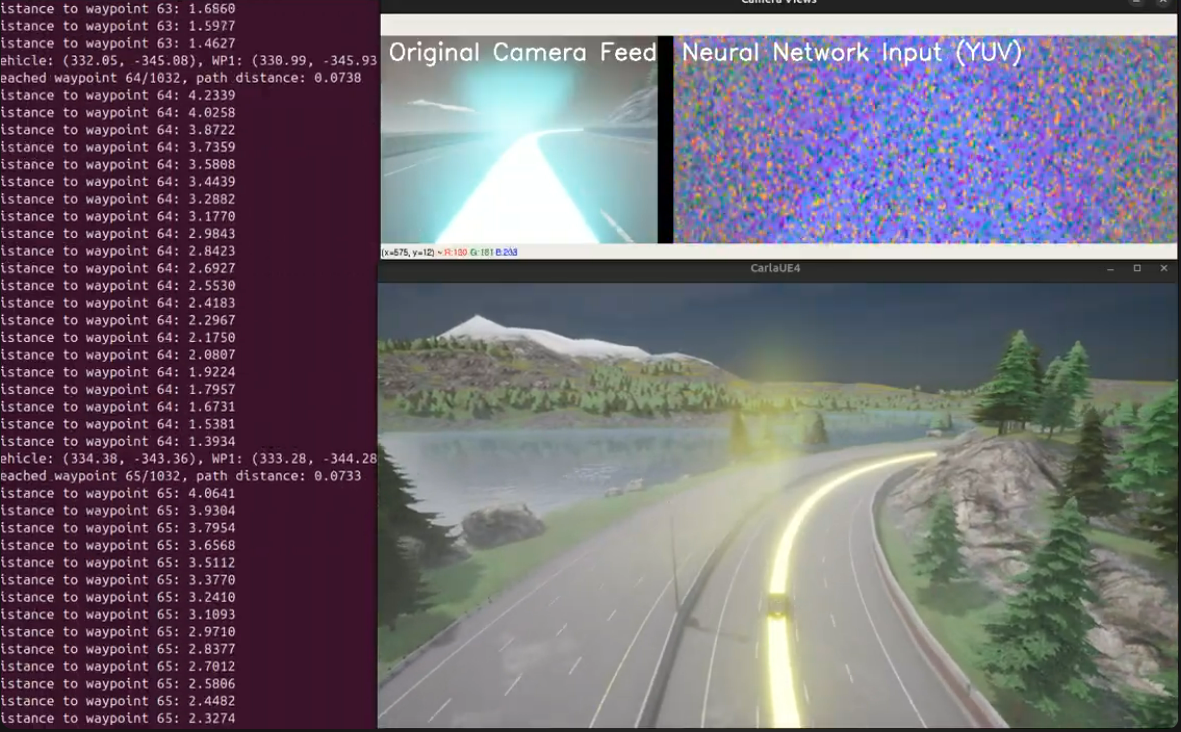
\includegraphics[width=0.75\textwidth]{Figures/Results/Exp239-30pc-noise-CNN-5-bin-bal-youtube.png}
    \caption{Experiment 239 YouTube video screenshot capture}
    \label{fig:Exp239-30pc-noise-CNN-5-bin-bal-youtube}
\end{figure}

%%%%%%%%%%%%%%%%%%%%%%%%%%%%%%%%%%%%%%%%%%%%%%%%%%%%%%%%%%%%%%%%%%%%%
% AVERAGE EUCLIDEAN DISTANCE TO CENTROIDS PRECEDING A LANE INVASION %
%%%%%%%%%%%%%%%%%%%%%%%%%%%%%%%%%%%%%%%%%%%%%%%%%%%%%%%%%%%%%%%%%%%%%

\textbf{Euclidean Distance to Centroids Preceding a Lane Invasion}
\label{res:ed_centroids_preceding_lane_invasion}

We are interested in observing if the Euclidean distance of a self-driving network softmax output to the predicted class centroid "spikes", that is presents a sharp increase, before a lane invasion is about to occur. As previously discussed, a lane invasion is defined when a vehicle's perpendicular distance to middle of the lane path is found to be greater than 0.85 units. 

Table \ref{tab:li_ed_comparison} presents average network softmax output Euclidean distance to class centroids for the last 10, 20 and 30 predictions (noting exactly one prediction is generated for every frame), where a lane invasion has occurred. Column \textbf{Exp} (integer) is the experiment ID , \textbf{Net} (string) is the network, \textbf{Noise} (integer percentage) is the percentage of pepper noise applied to the original vehicle's front facing camera image, \textbf{AvgED} (float) is the overall average Euclidean distance to predicted class centroid, \textbf{AvgED-LI-10} (float), \textbf{AvgED-LI-20} (float)  and \textbf{AvgED-LI-30} (float) is the same average, over the last 10, 20 and 30 predictions respectively, \textbf{FrCnt} (integer) is the frame count (number of predictions/frames) and \textbf{LI} (boolean) is the lane invasion boolean flag taking value T (true) when a lane invasion has occurred. Lane invasions occurred in all experiments reported in the table.

%The expectation would be that the

%%%%%%%%%%%%%%%%%%%%%%%%%%%%%%%%%%%%%%%%%%%%%%%%
% Average ED from softmax to centroids and Avg % 
% at 10, 20 and 30 frames from lane invasion   %
% selected results                             %
%%%%%%%%%%%%%%%%%%%%%%%%%%%%%%%%%%%%%%%%%%%%%%%%

% experiment 268

\begin{longtable}{@{}clcrrrrrcc@{}}
\toprule
Exp & Net & Bins & Noise & AvgED & AvgED-LI-10 & AvgED-LI-20 & AvgED-LI-30 & FrCnt & LI \\
\midrule
\endfirsthead
\toprule
Exp & Net & Bins & Noise & AvgED & AvgED-LI-10 & AvgED-LI-20 & AvgED-LI-30 & FrCnt & LI \\
\midrule
\endhead
240 & CNN & 5 & 40 & 0.6257 & 0.5616 & 0.5610 & 0.5631 & 10133 & T \\
241 & CNN & 5 & 50 & 0.6061 & 0.6215 & 0.6219 & 0.6273 & 10550 & T \\
242 & CNN & 5 & 55 & 0.5933 & 0.5135 & 0.5088 & 0.5192 & 4146 & T \\
243 & CNN & 5 & 60 & 0.5292 & 0.6206 & 0.6046 & 0.6041 & 369 & T \\
245 & ViT & 3 & 1 & 0.1063 & 0.3066 & 0.2268 & 0.1737 & 930 & T \\
246 & ViT & 3 & 2 & 0.0601 & 0.3339 & 0.2960 & 0.2088 & 144 & T \\
247 & ViT & 3 & 3 & 0.0617 & 0.3593 & 0.2924 & 0.2042 & 145 & T \\
248 & ViT & 3 & 4 & 0.0666 & 0.2934 & 0.2738 & 0.1912 & 144 & T \\
249 & ViT & 3 & 5 & 0.0697 & 0.2580 & 0.2349 & 0.1636 & 140 & T \\
250 & ViT & 3 & 7 & 0.0727 & 0.1358 & 0.2280 & 0.2591 & 271 & T \\
251 & ViT & 3 & 10 & 0.1530 & 0.3659 & 0.4113 & 0.3822 & 130 & T \\
252 & ViT & 3 & 20 & 0.2156 & 0.5062 & 0.4387 & 0.3874 & 108 & T \\
253 & ViT & 3 & 30 & 0.3234 & 0.5033 & 0.4594 & 0.4011 & 90 & T \\
254 & ViT & 3 & 40 & 0.4130 & 0.3171 & 0.3938 & 0.4251 & 58 & T \\
255 & ViT & 3 & 50 & 0.5513 & 0.5834 & 0.5582 & 0.5628 & 34 & T \\
256 & ViT & 5 & 10 & 0.4051 & 0.5901 & 0.5571 & 0.4842 & 164 & T \\
257 & ViT & 5 & 20 & 0.5415 & 0.6642 & 0.6754 & 0.6732 & 101 & T \\
258 & ViT & 5 & 30 & 0.5588 & 0.6995 & 0.6623 & 0.6020 & 120 & T \\
259 & ViT & 5 & 40 & 0.6238 & 0.7005 & 0.6296 & 0.6227 & 157 & T \\
260 & ViT & 5 & 50 & 0.7479 & 0.7522 & 0.7637 & 0.7658 & 114 & T \\
261 & ViT & 5 & 60 & 0.7627 & 0.7671 & 0.7598 & 0.7571 & 34 & T \\
\bottomrule
\caption{Comparison of Overall and Last 10, 20, 30 Predictions Euclidean Distance to Predicted Class Centroids for Experiments where Lane Invasion Occurred}
\label{tab:li_ed_comparison}
\end{longtable}


In Table \ref{tab:li_ed_comparison} the average Euclidean distance to predicted class centroid for the last 10, 20 and 30 predictions is examined, for experiments that resulted in lane invasions.

Table \ref{tab:experiment_stats} reports key metrics—average path distance (AvgPD), Euclidean distance (AvgED), Bhattacharyya distance (AvgBD), histogram intersection (AvgHI), KL divergence (AvgKL), frame count (FrCnt), and lane invasion status (LI)—across 27 experiments. Lane invasions (LI = T) occurred at noise levels of 40–60\% for CNN (5 bins) and 1–60\% for ViT (3/5 bins), with increased AvgED and AvgKL signaling prediction instability. Figure \ref{fig:combined_cnn_5bin_vit_3bin_vit_5bin_noise_distance_metrics} shows normalized metrics against noise (0, 10, 20, 30, 40, 50\%), with shaded regions indicating LI = T thresholds (e.g., Noise 40 for CNN, 5 bins; Noise 10 for ViT, 3/5 bins), highlighting metric degradation during invasions. Table~\ref{tab:youtube_links} provides YouTube video links for select experiments (e.g., Exp 261, ViT, 5 bins, 60\% noise), showing evidence of lane invasions.

Table~\ref{tab:li_ed_comparison} analyzes 21 LI = T experiments (Exps 240–243, 245–261), comparing the overall average Euclidean distance (AvgED) to averages for the last 10, 20, and 30 predictions (AvgED-LI-10, AvgED-LI-20, AvgED-LI-30), alongside noise and frame counts.

For CNN (5 bins), AvgED-LI-10 varies relative to AvgED (e.g., 0.5616 vs. 0.6257 for Exp 240; 0.6215 vs. 0.6061 for Exp 241), with AvgED-LI-20 and AvgED-LI-30 showing similar variability (e.g., 0.5610, 0.5631 for Exp 240; 0.6046, 0.6041 for Exp 243), suggesting inconsistent prediction errors near invasions.

For ViT (3 bins), AvgED-LI-10 is often higher than AvgED at low noise (e.g., 0.3066 vs. 0.1063 for Exp 245, Noise 1\%), but AvgED-LI-20 and AvgED-LI-30 decrease (e.g., 0.2268, 0.1737), indicating transient errors in the final 10 frames that stabilize over longer windows. At higher noise (e.g., Exp 252, Noise 20\%), AvgED-LI-10 remains high (0.5062), with AvgED-LI-20 and AvgED-LI-30 slightly lower (0.4387, 0.3874), suggesting sustained degradation.

For ViT (5 bins), AvgED-LI-10 consistently exceeds AvgED (e.g., 0.6642 vs. 0.5415 for Exp 257, Noise 20\%), with AvgED-LI-20 and AvgED-LI-30 varying (e.g., 0.6754, 0.6732 for Exp 257; 0.7598, 0.7571 for Exp 261), reflecting persistent prediction errors.

These findings highlight ViT's greater sensitivity to noise, with earlier lane invasions (Noise 1\% for 3 bins) and larger prediction errors in the final 10–30 frames compared to CNN (Noise 40\%), critical for assessing safety in noisy environments.

%%%%%%%%%%%%%%
% CONCLUSION %
%%%%%%%%%%%%%%

\section{Conclusion}

The work presented in this section demonstrates practical applications for quantifying uncertainty using the softmax space and softmax output distance to centroids. By first training two distinct neural network architectures, CNNs and ViTs, with synthetic datasets generated in a simulated environment presenting realistic conditions, the steering task was learned such that the simulated vehicles were able to drive around a figure of 8 circuit, where the lane to be driven in was segmented, without invading a neighbouring lane. Telemetry was taken to characterize acceptable driving. Noise was then added incrementally to front-facing vehicle camera images, before the noise-added images were presented to the steering network. 5 and 3 bin trained models were used, e.g. to predict steering classes "left", "straight" and "right", and prediction distances to class centroids recorded for all predictions. Lane invasions were determined by the distance of the vehicle to the middle path.

\section{Future Work}

The practical application illustrated in this work could be applied to any autonomous system relying on classification or regression for decision making. The use of Vision Language Models offers interesting research paths, be it in studying the softmax space and distances to centroids, or leveraging other metrics e.g. cosine similarity in the embedding space, to quantify and ultimately avoid hallucinations and bias.

\chapter{Background}

This chapter discusses the historical context of neural networks, followed by autonomous vehicle technology, trust, regulations, and safety methodologies.

\section{Neural Networks}
This section presents a discussion of key developments in the field that led to the vision models used in this research, as well as an overview of the architectures: Convolutional Neural Networks (CNNs), Vision Transformers (ViTs), and Vision Language Models (VLMs).

Modern neural networks trace their origins to the logical neuron model proposed by McCulloch and Pitts, which demonstrated that simple binary threshold units could implement any logical function (\cite{mcculloch1943logical}). This foundational work established a mathematical framework for computational models of the mind. Rosenblatt's Perceptron introduced learning through adjustable weights and error correction, establishing the first practical machine learning algorithm (\cite{rosenblatt1958perceptron}).
Biological inspiration drove architectural advances. Hubel and Wiesel's research on the visual cortex revealed hierarchical feature detection in cat neurons, with simple cells responding to edges and complex cells to abstract patterns (\cite{hubel1962receptive}). Fukushima's Neocognitron directly implemented this hierarchy using S-cells for feature extraction and C-cells for spatial pooling, laying the foundation for modern convolutional neural networks (CNNs) (\cite{fukushima1980neocognitron}).

Subsequent CNN advancements, such as LeCun's LeNet for handwritten digit recognition (\cite{lecun1998gradient}) and AlexNet (\cite{krizhevsky2012imagenet}) also for image classification, solidified CNNs as a standard tool in the computer vision and deep learning toolbox, enabling end-to-end learning for self-driving cars (\cite{bojarski2016end}).
Efficient training emerged through backpropagation, first formalized by Linnainmaa in the context of automatic differentiation (\cite{linnainmaa1970cumulative}) and later applied to neural networks by Werbos (\cite{werbos1974beyond}). Cybenko's Universal Approximation Theorem proved that feedforward neural networks could approximate any continuous function, providing a theoretical justification for their expressive power (\cite{cybenko1989approximation}).

Modern training relies on key techniques. The Adam optimizer provides adaptive learning rates for faster convergence (\cite{kingma2014adam}). Dropout prevents overfitting by randomly deactivating neurons during training (\cite{srivastava2014dropout}). Early stopping halts training when validation performance degrades (\cite{goodfellow2016deep_early_stopping}).
Contemporary architectures address diverse computational challenges. CNNs utilize hierarchical convolution and pooling for spatial feature extraction (\cite{lecun1998gradient,krizhevsky2012imagenet}). Vision Transformers process images as patch sequences using global self-attention mechanisms (\cite{dosovitskiy2021image}). Vision-language models, such as Qwen-VL (\cite{bai2023qwen}) and DeepSeek-VL (\cite{zeng2024deepseek}), combine visual encoders with language models through cross-attention adapters, enabling multimodal understanding.

\section{SAE Autonomy Levels}

The Society of Automotive Engineers (SAE) defines six levels of driving automation, from no automation (Level 0) to full automation (Level 5), as outlined in the J3016 standard (\cite{SAEJ3016}). These levels categorize the extent to which a vehicle can perform the dynamic driving task (DDT) and the degree of human intervention required.

Levels 0--2 involve human drivers maintaining primary control, with increasing assistance from advanced driver-assistance systems (ADAS). Levels 3--5 represent conditional to full automation, where the vehicle assumes complete DDT responsibility under specific conditions or universally, progressively eliminating the need for human intervention. The table below summarizes the SAE levels, their capabilities, and human driver requirements.

\begin{table}[h]
\centering
\caption{SAE Levels of Driving Automation}
\begin{tabular}{|c|p{6cm}|p{6cm}|}
\hline
\textbf{Level} & \textbf{Description} & \textbf{Human Driver Requirement} \\
\hline
0 & No automation; human performs all driving tasks & Full control and monitoring \\
\hline
1 & Driver assistance; system handles specific tasks (e.g., steering or acceleration) & Continuous monitoring and control \\
\hline
2 & Partial automation; system manages steering and acceleration but requires human oversight & Constant supervision; ready to intervene \\
\hline
3 & Conditional automation; vehicle performs DDT in specific conditions (e.g., highway) & Present; must respond to system requests \\
\hline
4 & High automation; vehicle performs DDT within operational design domain without human input & None within domain; vehicle self-manages \\
\hline
5 & Full automation; vehicle performs DDT in all conditions without human involvement & None; no human driver required \\
\hline
\end{tabular}
\end{table}

\section{Global State of Autonomous Vehicle Adoption in 2025}

The global transition to autonomous vehicles (AVs), encompassing SAE Levels 3 to 5, is reshaping transportation through advancements in technology, regulation, infrastructure, and societal integration. The 2025 Global Autonomous Vehicle Adoption Index provides a standardized measure of AV adoption across regions, evaluating market penetration, regulatory frameworks, infrastructure readiness, consumer trust, and industry ecosystems (\cite{KPMG2018}).

North America and Asia-Pacific lead the global landscape, driven by robust private-sector innovation and state-directed strategies, respectively. Europe follows with a safety-focused approach (\cite{GOVUK2024}), while the Middle East, Africa, and Latin America lag due to infrastructural and regulatory constraints, though select markets show potential for rapid advancement through targeted investments (\cite{DubaiLaw2023}).

Regional disparities highlight divergent pathways to AV leadership. North America's dominance stems from extensive R\&D and widespread adoption of ADAS, but fragmented regulations hinder national scaling (\cite{NCSL2025}). Asia-Pacific, particularly China, benefits from cohesive national policies and significant infrastructure investments, such as 5G networks and smart roadways, enabling rapid deployment (\cite{KPMG2018}). Europe's comprehensive regulatory frameworks prioritize safety but slow iterative testing, potentially ceding early market share (\cite{GOVUK2024}). Emerging markets in the Middle East, like the UAE, leverage smart city initiatives to create AV-ready environments, while most African and Latin American nations face foundational challenges in connectivity and governance (\cite{DubaiLaw2023}).

Consumer trust remains a universal barrier to mass adoption, with public scepticism about safety and control persisting despite technological progress (\cite{PatentPC2025a,Deloitte2024}). This trust deficit, most pronounced in Western markets, necessitates transparent safety validation and public education to align perceptions with engineering realities.

Regulatory models also shape adoption trajectories. North America's decentralized approach fosters innovation but lacks cohesion (\cite{NCSL2025}). Asia-Pacific's top-down model accelerates deployment. Europe's consensus-driven framework emphasizes long-term trust over speed (\cite{GOVUK2024}). The symbiotic relationship between AVs and electric vehicles (EVs) further influences progress, as EV infrastructure supports the shared technological foundation of autonomous systems (\cite{IEA2024}).

Strategic imperatives for stakeholders include harmonizing regulations, enhancing infrastructure, and addressing consumer concerns. Policymakers must prioritize clear, unified legal frameworks to reduce compliance burdens and enable scaling (\cite{NCSL2025}). Industry leaders should shift focus from technological development to trust-building through public demonstrations and region-specific strategies (\cite{Deloitte2024}). Emerging markets can attract investment by creating controlled AV testing zones, leveraging their lack of legacy infrastructure to bypass incremental development (\cite{DubaiLaw2023}). Despite data limitations and urban biases in current assessments, ongoing refinements to metrics like cybersecurity and socioeconomic impacts will enhance future evaluations of this transformative mobility landscape (\cite{KPMG2018}).

\section{Societal Impact of Autonomous Vehicles and Systems}

Autonomous vehicles (AVs) and systems promise transformative societal benefits by enhancing safety, mobility, and efficiency. By mitigating human error, the primary cause of traffic accidents, AVs could significantly reduce road fatalities and healthcare costs (\cite{Fagnant2015}). They offer improved mobility for groups like the elderly and disabled, fostering social inclusion (\cite{Harper2016}). Optimized driving patterns and integration with electric vehicles may reduce emissions, though increased vehicle usage could offset these gains (\cite{Greenblatt2015}).

The economic impact of AVs and autonomous systems is likely to be substantial. While they may create new job opportunities in technology and related fields, there are concerns about job displacement, particularly in transportation-related industries (\cite{Autor2015}). The trucking and taxi industries, for instance, could face significant disruption. Some argue that the automation of monotonous roles would benefit society overall, freeing human potential for more creative and fulfilling endeavours (\cite{Picone2025}).

\section{Trust in Autonomous Vehicles}

Trust in AVs encompasses reliability, safety, security, and ethical decision-making. For AVs to be widely accepted and integrated into everyday life, it is essential to address these concerns comprehensively.

\textbf{Reliability} refers to the consistent performance of AVs under various conditions. For consumers, the reliability of AVs is paramount as it determines the vehicle's dependability in routine operations and unexpected scenarios. Issues such as software bugs, hardware malfunctions, or failures in sensor systems can significantly undermine trust. Studies indicate that consumers are particularly wary of AVs' ability to handle adverse weather conditions or complex traffic situations (\cite{gogoll2017}).

\textbf{Safety} is the most significant factor influencing trust in AVs. This aspect covers the vehicle's ability to avoid accidents and protect passengers and pedestrians. According to the National Highway Traffic Safety Administration (NHTSA), while AVs have the potential to reduce accidents caused by human error, there is a need for rigorous testing and validation to ensure their safety in real-world conditions \cite{nhtsa2020}. Incidents involving AVs, such as the fatal Uber crash in 2018, have heightened public concern and scepticism about the technology's readiness (\cite{goodall2016}).

\textbf{Security} concerns involve the protection of AVs from cyber-attacks. As AVs rely heavily on software and connectivity for their operation, they are vulnerable to hacking, which could lead to disastrous consequences. Ensuring robust cybersecurity measures is essential to protect against unauthorized access and data breaches. The European Union Agency for Cybersecurity (ENISA) has emphasized the importance of cybersecurity in AVs, recommending the implementation of stringent security protocols and regular updates to counter emerging threats (\cite{enisa2020}).

\textbf{Ethical decision-making} in AVs involves programming these vehicles to make decisions during unavoidable accidents. This aspect raises moral and philosophical questions about how AVs should prioritize lives and property in critical situations. The "trolley problem" is a classic example often discussed in the context of AV ethics, where the vehicle must choose between two harmful outcomes (\cite{Lin2015}). Public trust in AVs significantly depends on transparent and ethically sound decision-making frameworks that align with societal values.

Consumers are primarily concerned with reliability, safety, security, and ethical decision-making. Additionally, there is apprehension about the lack of control and the ability to intervene in the vehicle's operation during emergencies. Regulators focus on establishing comprehensive guidelines and standards to ensure safe deployment. They are concerned with liability issues, the adequacy of current infrastructure to support AV technology, and the long-term societal impacts of widespread AV adoption (\cite{litman2020}).

Building trust in AVs requires addressing these concerns comprehensively. Both consumer acceptance and regulatory approval hinge on demonstrating that AVs can operate dependably and safely while adhering to ethical standards. Ongoing research, transparent communication, and robust regulatory frameworks are crucial to fostering trust in this transformative technology.

\section{State of the Art}

AV technology has evolved significantly in the past decade, moving from conceptual designs to real-world deployments. Major technology companies and traditional auto-makers are investing heavily in this field, leading to a diverse and competitive landscape.

Currently, most commercially available autonomous systems operate at SAE Level 2 or Level 3 autonomy (\cite{SAE2021}). These systems can control steering, acceleration, and braking in specific scenarios but require human oversight. However, several companies are actively testing Level 4 and Level 5 systems, which promise full autonomy in most or all driving conditions (\cite{Yurtsever2020}).

Waymo, a subsidiary of Alphabet Inc., is one of the leaders in the AV field. Their self-driving taxi service, Waymo One, has been operational in Phoenix, Arizona since 2018, recently expanding to San Francisco (\cite{Waymo2023}). Tesla, with its Autopilot and Full Self-Driving (FSD) systems, has the largest fleet of AVs, providing vast amounts of real-world data (\cite{Tesla2023}).

Other major players include traditional auto-makers like General Motors (through its Cruise subsidiary), Ford, and Volkswagen, as well as technology companies like Uber, Aptiv, and Baidu (\cite{Koopman2019}). These companies are employing a variety of sensing technologies, including LIDAR, radar, cameras, and ultrasonic sensors, often in combination (\cite{Yurtsever2020}).

Recent advancements in the field include improved perception systems capable of detecting and classifying objects with greater accuracy, even in challenging weather conditions (\cite{Grigorescu2020}). There have also been significant developments in decision-making algorithms, with the incorporation of deep learning and reinforcement learning (\cite{Kiran2021}).

Despite these advancements, several challenges remain. These include ensuring safety in numerous edge cases, sometimes referred to as "the long tail", gaining regulatory approval, addressing ethical concerns, and achieving public acceptance (\cite{Koopman2019}). The ability of AVs to operate in diverse environments and weather conditions, as well as their interaction with human-driven vehicles and pedestrians, are ongoing areas of research and development (\cite{Yurtsever2020}).

It is clear that AVs have the potential to disrupt transportation. However, the timeline for widespread adoption of fully autonomous vehicles remains uncertain and dependent on overcoming technical, regulatory, and social challenges (\cite{Litman2023}).

\section{Regulatory Landscape for Autonomous Vehicles and Systems}

The regulatory environment for Autonomous Vehicles (AVs) and other autonomous systems is evolving rapidly, with different regions adopting varied approaches. This diversity in regulation reflects the complex challenges of balancing innovation, safety, and public interest in the face of rapidly advancing technology.

In the United States, the regulatory approach has been largely decentralized, with individual states taking the lead in AV regulation. The National Highway Traffic Safety Administration (NHTSA) has provided guidelines for AV testing and deployment, but these are largely voluntary (\cite{nhtsa2020}). This flexible approach has facilitated extensive AV testing, but it has also led to a patchwork of regulations that may complicate interstate operations.

The European Union has taken a more centralized approach, working towards harmonized regulations across member states. The EU has introduced the AV-Ready initiative, aiming to create a comprehensive regulatory framework for AVs. This includes updates to type-approval regulations and efforts to address liability and ethical issues.

In Asia, countries like China, Japan, and Singapore have been proactive in creating regulatory frameworks for AVs. China, in particular, has implemented national guidelines for AV testing and is working on standards for AV deployment. Singapore has created a flexible regulatory framework that allows for rapid adaptation to technological advancements (\cite{Taeihagh2019}).

Globally, there's a growing recognition of the need for international cooperation in AV regulation. The United Nations Economic Commission for Europe (UNECE) has been working on amendments to the Vienna Convention on Road Traffic to accommodate AVs.

For broader autonomous systems, regulatory approaches vary significantly depending on the application domain. In aviation, for instance, regulations for autonomous drones are more developed than those for autonomous passenger aircraft. In healthcare, regulatory bodies like the FDA in the US are developing frameworks for AI and machine learning in medical devices.

A key challenge across all regions is keeping pace with rapid technological advancements. Regulators are increasingly adopting "adaptive" or "agile" regulatory approaches that allow for more flexibility and rapid updates. These approaches aim to balance the need for safety and accountability with the desire to foster innovation.

Another common theme is the shift towards performance-based regulations rather than prescriptive rules. This approach focuses on defining desired outcomes rather than specifying exact methods, allowing for technological innovation while maintaining safety standards.

Ethics and liability remain challenging areas for regulators globally. Questions about how to encode ethical decision-making into autonomous systems and how to assign liability in case of accidents are still largely unresolved (\cite{Awad2018}).

As the technology continues to evolve, regulatory frameworks will need to adapt. The challenge for policymakers will be to create regulations that ensure safety and public trust while allowing for continued innovation in the field of autonomous systems.

\section{Safety Methodologies for Autonomous Vehicles}

The assessment and verification of safety in Autonomous Vehicles (AVs) present unique challenges that necessitate both the adaptation of traditional automotive safety practices and the development of novel methodologies. This section provides an overview of current approaches; detailed technical methodologies will be presented in the methodology chapter. Current approaches encompass a wide range of techniques, each with its own strengths and limitations.

One prevalent methodology is scenario-based testing, where AVs are evaluated against a comprehensive set of pre-defined driving scenarios (\cite{Feng2021}). These scenarios aim to cover a broad spectrum of driving conditions, from routine situations to rare, high-risk events. However, the vast number of possible scenarios makes exhaustive testing impractical, leading to the development of methods for intelligent scenario selection and generation (\cite{Koren2018}).

Formal methods and model checking represent another critical approach in AV safety assessment. These techniques involve creating mathematical models of AV systems and their environments, then using automated tools to verify that specific safety properties are consistently maintained (\cite{Luckcuck2019}). While powerful, these methods can be computationally intensive and may not scale to highly complex systems.

Simulation-based testing plays a crucial role in AV safety assessment. Advanced simulators enable the testing of AVs in virtual environments, allowing for the evaluation of numerous scenarios without the risks associated with real-world testing (\cite{Dosovitskiy2017}). However, ensuring that simulations accurately represent real-world conditions remains a significant challenge.

This study focuses on the data presented to AV models at runtime and the use of simulators, both critical for decision-making and safety assurance. Analysing runtime data inputs and simulator-based testing will address gaps in current methodologies, enhancing safety validation.

\chapter{Related Work}
\label{chap:related_work}

This chapter reviews key literature relevant to distance-based uncertainty quantification and failure detection in neural networks, focusing on softmax-based approaches and classification reliability assessment.

\section{Softmax-Centroid Relationships}

Hess et al. \cite{HessEtAl2020} argue that softmax-based neural network classification is equivalent to k-means clustering in the transformed feature space. Their work demonstrates that the softmax function partitions the input space into cones, with each cone corresponding to a class centroid at equal distance from the origin.

However, there is a fundamental difference between training a neural network and k-means clustering. In neural network training, the actual point defined by softmax output scores moves during training, i.e., while the network is learning, parameters are being adjusted to improve accuracy given an objective function. The predictions move through the $n$-dimensional clustering space. At the beginning of the training process, where accuracy is typically lower than at the end, both the predictions (softmax outputs) and the centroids (softmax output averages) are in a state of flux, until training stops and the network's weights and biases are fixed.

In contrast, k-means clustering operates on fixed data. The points in any number of dimensions $n$ are fixed at the outset, and the centroids are the entities that move during the clustering process. Therefore, the process of training a neural network is not equivalent to k-means clustering.

The first author of \cite{HessEtAl2020} acknowledges that "It's probably misleading to call the centers centroids, because they are strictly speaking no centroids [sic]" and that "The proof in the arXiv version has a flaw, but we can show a similar result, which I hope to publish some time" \cite{hess2025email}.

\section{Error Detection Methodologies}

Qiu and Miikkulainen \cite{QiuMiikkulainen2022} propose RED (Residual-based Error Detection), which uses Gaussian Processes to detect misclassification errors. Their method builds on RIO (Residual prediction with Input/Output kernel) and provides both detection scores and uncertainty estimates for these scores.

RED shares our goal of identifying unreliable predictions, but employs a fundamentally different approach. RED constructs residuals between target detection scores and maximum class probabilities, requiring additional Gaussian Process training. In contrast, the distance-to-centroid approach requires only computing Euclidean distances to pre-calculated centroids, offering computational simplicity.

Corbière et al. \cite{Corbiere2019} address failure prediction by introducing True Class Probability (TCP) as an alternative to Maximum Class Probability (MCP). Their ConfidNet architecture learns to predict TCP during training using an L2 loss function, demonstrating superior separation between correct and incorrect predictions compared to traditional confidence measures.

Both ConfidNet and our work recognize that maximum softmax probability is insufficient for reliable confidence assessment. ConfidNet learns confidence through a separate neural network, while the distance-based approach leverages geometric properties of the softmax space directly. The distance method requires no additional training and provides immediate confidence assessment based on distance thresholds to class centroids.

\section{Evaluation Frameworks}

Jaeger et al. \cite{Jaeger2022} critique current evaluation practices for failure detection, identifying inconsistencies in task definitions, limited failure source coverage, and evaluation-purpose misalignment. They propose unified evaluation using Area under the Risk-Coverage-Curve (AURC) and Confidence Scoring Functions (CSF).

Their work validates the need for consistent evaluation methodologies that our work addresses through systematic evaluation and comparison across multiple distance metrics (Euclidean, Cosine, Mahalanobis, etc.) and datasets (MNIST, CIFAR-10, etc.). This validation establishes Euclidean distance as a reasonable metric choice, i.e., not the best (cosine similarity performs better) but far from the worst (entropy performs worse). The distance-based approach provides a unified framework applicable across different architectures without requiring method-specific modifications.

\section{Prototype-Based and Distance Methods}

Center Loss \cite{Wen2016} encourages intra-class compactness in feature spaces through an auxiliary penalty term, promoting geometric clustering around learned centroids. Prototypical Networks \cite{Snell2017} demonstrate feature-space prototyping effectiveness for few-shot learning by computing class prototypes as arithmetic means of support set embeddings and performing classification via nearest prototype assignment.

Trust Score \cite{Jiang2018} measures agreement between a classifier's prediction and a modified nearest-neighbor classifier in the learned feature space, providing confidence measures less susceptible to adversarial examples. Monte Carlo Dropout \cite{Gal2016} provides Bayesian uncertainty estimation through multiple forward passes with different dropout masks, treating dropout as a variational approximation to a Gaussian process.

Our methodology operates directly in the softmax output space rather than feature spaces, offering architecture independence. The method demonstrates that simple Euclidean distance to class centroids provides effective confidence assessment while maintaining computational efficiency compared to more complex distance-based approaches.

\section{Calibration Methods}

Temperature scaling \cite{Guo2017} provides post-hoc calibration by optimizing a single parameter on validation sets to minimize negative log-likelihood. Modern neural networks often produce poorly calibrated, overconfident predictions, which makes calibration relevant to confidence assessment methods. The relationship between calibration and prototype quality is particularly important for softmax-based methods where well-calibrated probability distributions are essential for meaningful analysis.

\section{Summary}

The reviewed literature establishes theoretical foundations for centroid-based neural network analysis and demonstrates various approaches to confidence estimation and error detection. The distance-to-centroid methodology builds upon these foundations while offering a lightweight, architecture-independent approach to uncertainty quantification in neural network predictions.

While existing methods provide valuable frameworks for uncertainty quantification and error detection, several gaps remain. Most approaches require additional training, operate in feature spaces rather than output spaces, or are architecture-specific. This thesis addresses these gaps by demonstrating that simple distance metrics in softmax space provide effective uncertainty quantification across multiple architectures (CNNs, ViTs, VLMs) and application domains (classification, regression in autonomous driving scenarios).


% METHODS
\chapter{Methods}
\label{chap:methods}

This section describes the methods used to develop and validate distance-based safety assessment for autonomous systems. Methods cover computational infrastructure, simulation environment, distance metrics, noise perturbation, dataset generation, neural network architectures, training protocols, softmax clustering algorithm, regression-to-classification transformation, and Vision Language Model implementation.

\section{Experimental Setup}

\subsection{Computational Infrastructure}
\label{methods:hardware}

All code implementations were developed in Python (\cite{python}) using standard libraries (NumPy, OpenCV, Matplotlib) with shell scripting for batch job execution on the City St George's, University of London, School of Science and Technology HPC (high-performance computing cluster). The remote compute infrastructure comprised 19 GPU cards across five nodes with a total of 872GB GPU memory, where a maximum of 8 GPU cards from the pool were used concurrently. A local workstation was used for code development, network training and testing, as well as running the CARLA simulator (\cite{dosovitskiy17}). GitHub (\cite{github}) was used as the code repository.

\begin{longtable}{@{}lcc@{}}
\toprule
Node & GPU Configuration & Total Memory \\
\midrule
\endfirsthead
\toprule
Node & GPU Configuration & Total Memory \\
\midrule
\endhead
gpu01 & 3 × Quadro RTX 8000 & 138GB \\
gpu02 & 8 × NVIDIA A100-PCIE-40GB & 320GB \\
gpu03 & 2 × NVIDIA A100 80GB PCIe & 160GB \\
gpu04 & 4 × NVIDIA A100 80GB PCIe & 320GB \\
gpu05 & 2 × NVIDIA A100 80GB PCIe & 160GB \\
\midrule
\textbf{Total} & \textbf{19 cards} & \textbf{872GB} \\
\bottomrule
\caption{CSGULSST HPC GPU Infrastructure}
\label{tab:hpc_hardware}
\end{longtable}

The local development workstation utilized a GeForce GTX 1060 6GB, later upgraded to an RTX 3060 12GB.

\begin{longtable}{@{}lcc@{}}
\toprule
Configuration & GPU Model & Memory \\
\midrule
\endfirsthead
\toprule
Configuration & GPU Model & Memory \\
\midrule
\endhead
Initial Setup & GeForce GTX 1060 & 6GB \\
Upgraded Setup & GeForce RTX 3060 & 12GB \\
\bottomrule
\caption{Local Development Workstation GPU Configuration}
\label{tab:local_hardware}
\end{longtable}

\subsection{CARLA Simulator}
\label{methods:carla}

\begin{figure}[h]
\centering
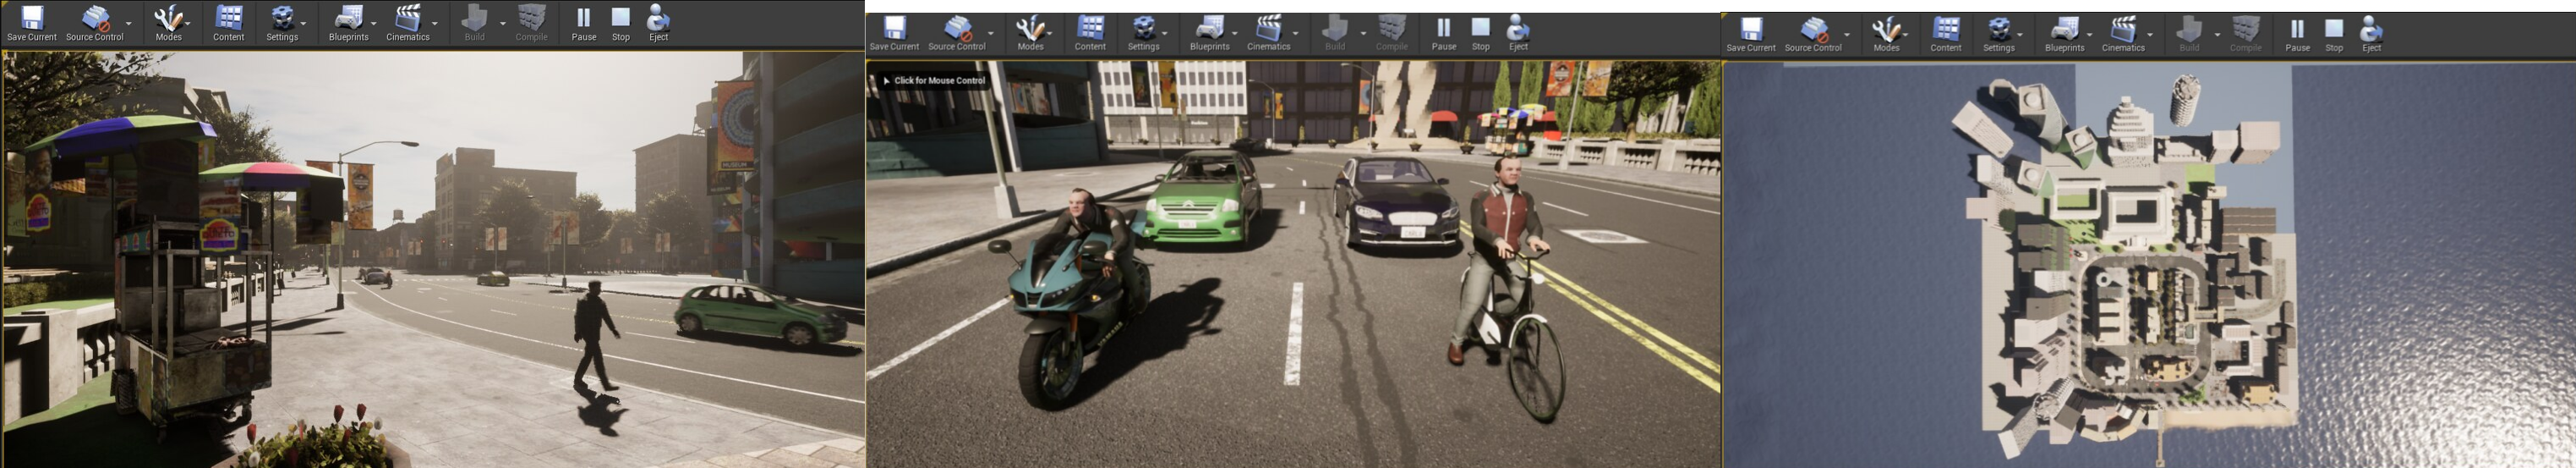
\includegraphics[width=0.99\textwidth]{Figures/Methods/CarlaTown10.png}
\caption{From left to right: a running simulation in the CARLA Town10 map with 60 vehicles and 100 pedestrians; a similar simulation showing motorcyclist, cyclist and two vehicles waiting at traffic lights; and a bird's eye view of CARLA Town10 map.}
\label{fig:CarlaTown10}
\end{figure}

CARLA (Car Learning to Act) is an open-source simulator (Figure \ref{fig:CarlaTown10}) for autonomous driving research, built on Unreal Engine (\cite{unrealengine}). The Python API provides a client-server architecture where the client establishes a TCP connection to the simulator instance. The client retrieves the world object representing the simulation environment and can access various components for controlling autonomous behaviour. World settings can be modified to enable synchronous or asynchronous execution modes, with synchronous mode providing deterministic simulation steps through world tick calls. The API exposes a blueprint library system for actor spawning, where vehicle and pedestrian blueprints are filtered and configured with attributes such as colour and driver appearance. Vehicles and pedestrians can be spawned at spawn points, which in turn are retrieved from the world's navigation mesh. The simulation loop maintains real-time execution through continuous world ticking. Weather conditions including cloudiness, precipitation, wind intensity, fog density, and surface wetness can be dynamically controlled. Solar positioning is adjustable through azimuth and altitude angles. The framework supports autonomous driving agents which were not used, a custom agent was built for this study.

\section{Datasets and Preprocessing}

\subsection{Self-Driving Training Datasets}
\label{methods:carla_gen_train_datasets}

The self-driving training dataset generation process operates through automated CARLA simulation runs. To define a route, a set of pre-defined waypoints, retrievable from the town map mesh, are examined. A waypoint has \texttt{road\_id} and \texttt{lane\_id} attributes. The figure of 8 expressway around Town04 map (Figure \ref{fig:Town04FigureOfEight}) can be identified by selecting \texttt{road\_id}s with 4 \texttt{lane\_id}s, then ordering the \texttt{road\_id}s in a list that will result in the desired sequence of waypoints. A vehicle is spawned at the first waypoint of the sequence with an RGB camera mounted at a configurable position and orientation.
The simulated vehicle follows the road waypoint sequence along 28 road\_id segments, using waypoints at 1 unit of distance intervals (for regression and 15 bin quantized classification) and 3 units of distance intervals (5 and 3 bin quantized classification). Permanent waypoint lines are drawn for lane segmentation. The steering algorithm computes the angular difference between the vehicle's transform orientation and the nearest waypoint's transform orientation. This delta is applied as a steering correction to align the vehicle path with the road centre line.

\begin{figure}[h]
\centering
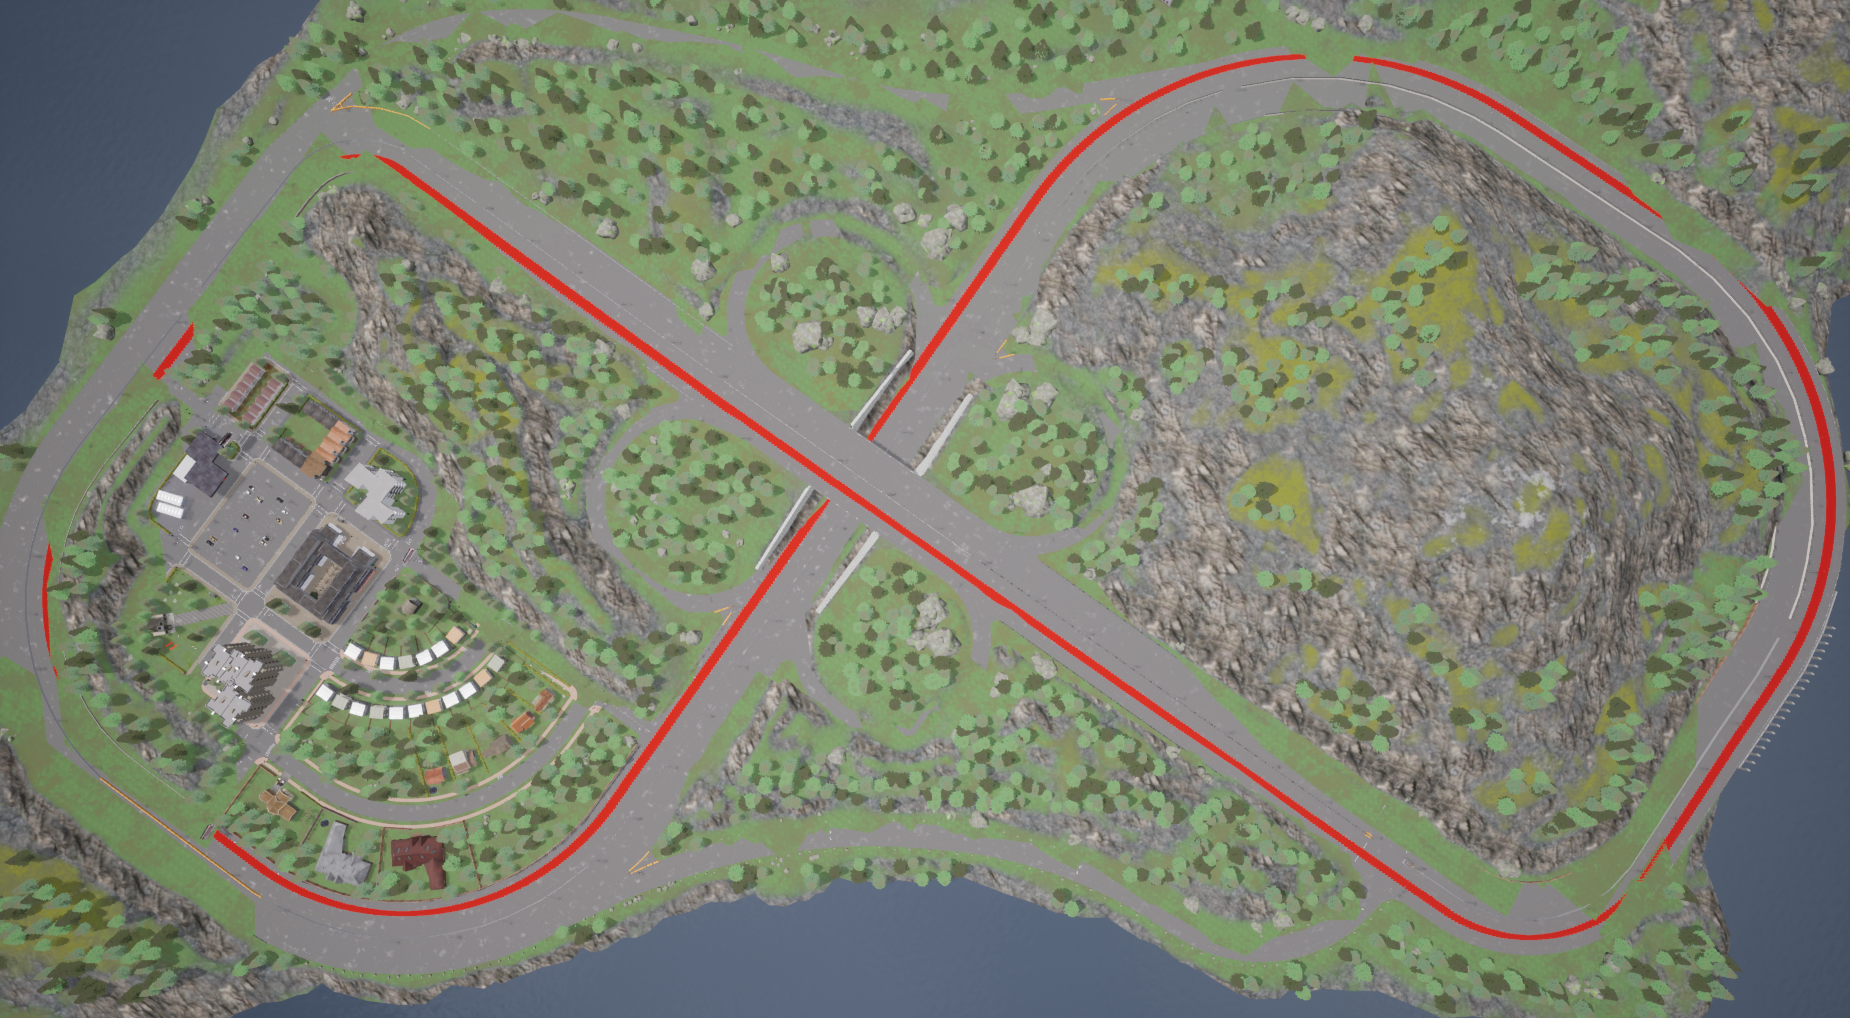
\includegraphics[width=0.99\textwidth]{Figures/Methods/Town04FigureOfEight.png}
\caption{The CARLA Town04 Figure-of-eight circuit. The path is set on lane id -2, that is the second from left to right, on the right hand lane. The circuit is composed by determining which road sections comprise the desired route, then concatenating the waypoints of each section sequentially to form a full lap.}
\label{fig:Town04FigureOfEight}
\end{figure}

Two dataset generation modes were developed for this study: continuous regression mode saves the raw steering angle delta (steering adjustment from one waypoint to the next) as the label, while quantized classification mode approximates and truncates the continuous delta to the nearest of 15, 5 or 3 predefined bin values ranging from -0.065 to 0.065 in CARLA's normalized control space. This corresponds to approximately $\pm$4.5 degrees of the vehicle's $\pm$70 degree steering range, noting that the interval $\pm$4.5 degrees is sufficient to steer the vehicle around the circuit without lane invasions.
Data collection occurs at each simulation tick, capturing RGB images with steering angles embedded in timestamped filenames e.g. 20250314\_094117\_214470\_steering\_-0.0167.jpg (steering value -0.0167 corresponds to -1.17 degrees, that is vehicle is steering slightly left) such that alphabetical order will correspond to the order image file was generated. Ground truth safety distances are computed as perpendicular distances from vehicle position to the lane centre line defined by consecutive waypoint pairs. Orthogonal distances from the centre line exceeding 0.85 units indicate lane invasion events. Each complete figure of eight lap generates approximately 28,000 labelled images under synchronous mode execution.

\begin{figure}[h!]
\centering
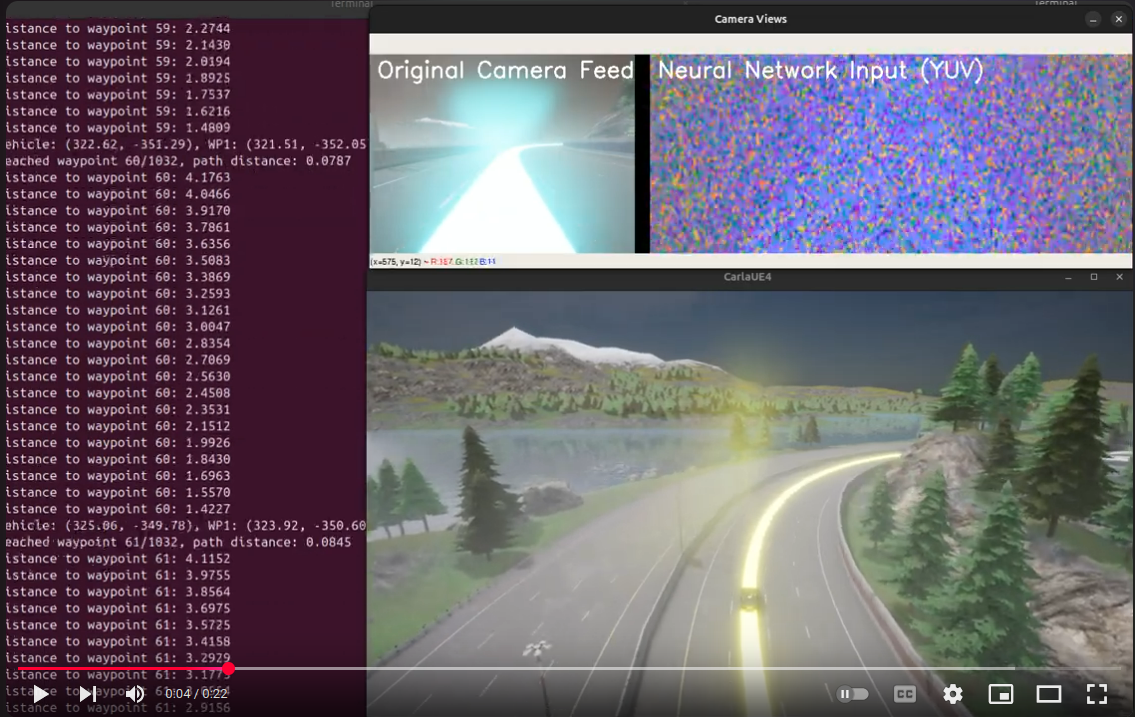
\includegraphics[width=0.99\textwidth]{Figures/Results/youtubeidCzJlbYX0CnQ_experiment239_30pc_pepper_noise_5bin_cnn_balanced.png}
\caption{A CARLA simulation where the vehicle is driven by a CNN trained on a 5 bin balanced dataset, and subject to 30\% pepper noise. The column on the left are debug prints of distances to the nearest waypoints, virtual anchors and part of a mesh in the CARLA world when actors e.g. vehicles and pedestrians, can be spawned/created/instantiated, the larger figure on the bottom left is the simulator from the "spectator" perspective. The spectator is this case is set to track the vehicle at every "tick", that is, every update of the CARLA world, where spectator is set 35 units of distance along the x axis (behind the vehicle) and 20 units of distances along the z axis (above the simulated vehicle), while the pitch (rotation along the lateral axis) set to -15 degrees, that is the spectator is looking down. There is no translation along the y axis, and no rotation along the vertical axis (yaw) or longitudinal axis (roll). The image on the top left of the simulator is the one frame capture from front facing vehicle camera and the image on the top right is the camera image cropped to exclude the section above the horizon and resized to 200w x 66h pixels, then moved from RGB to YUV space.}
\label{fig:youtubeidCzJlbYX0CnQ_experiment239_30pc_pepper_noise_5bin_cnn_balanced}
\end{figure}

%%%%%%%%%%%%%%%%%%%%%%%%%
% SELF-DRIVING DATASETS %
%%%%%%%%%%%%%%%%%%%%%%%%%

% \subsection{Self-Driving Datasets}

\begin{figure}[h]
\centering
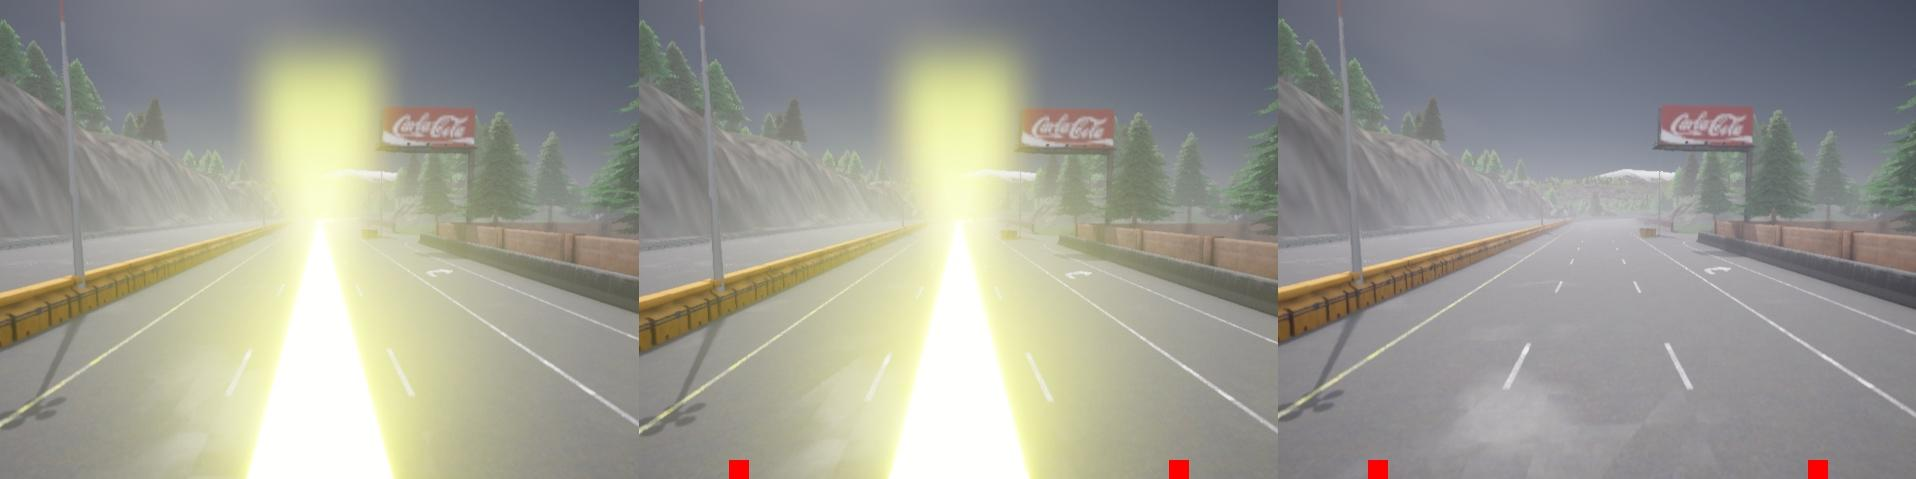
\includegraphics[width=0.99\textwidth]{Figures/Methods/carla_dataset_seg_segfid_fid.jpg}
\caption{Images captured with a CARLA simulated vehicle front facing camera, from left to right, with road segmentation, road segmentation and fiducial markers and fiducial markers only, where the most commonly used image type used in this study were images with road segmentation only (left).}
\label{fig:carla_dataset_seg_segfid_fid}
\end{figure}

% We capture datasets (with images as displayed in Figure \ref{fig:carla_dataset_seg_segfid_fid}) using the process described in subsection \ref{methods:carla_gen_train_datasets}. 
Datasets may have continuous or quantized steering angle labels, additionally the images could be raw (no markers), contain lane segmentation, contain lane segmentation and fiducial markers, or contain fiducial markers only.
 
Lane segmentation for autonomous driving has evolved from classical image processing to deep learning-based, pixel-wise semantic segmentation, often using UNet-like architectures. However, to meet real-time demands and handle occlusions, recent methods reframe the task as a row-based classification problem using global features, achieving significantly higher speeds \cite{qin2020ultra}. Conversely, fiducial markers like AprilTag provide robust 6-DOF pose estimation for robotics by introducing engineered, high-contrast patterns into the environment, simplifying perception into a problem of detecting known landmarks and solving for camera pose \cite{olson2011tags}.

Lane segmentation is a staple in self-driving, and in this study lane segmentation was generated by using a specific feature of the CARLA simulator - connecting waypoints with markers, although road and lane marker segmentation itself does exist as a feature in CARLA, the feature is unable to segment a single lane.

%%%%%%%%%%%%%%%%%%%%%%%%%%%%%%%%%%%%%%%
% SELF-DRIVING DATASETS - REGRESSSION %
%%%%%%%%%%%%%%%%%%%%%%%%%%%%%%%%%%%%%%%

%\subsubsection{Self-Driving Datasets - Regression}

\textbf{Regression:} Three regression dataset variants predict continuous steering angle values from camera images:

\textbf{Vanilla} uses raw camera images as input with continuous steering angle targets.

\textbf{Segmented} - Vanilla plus lane segmentation.

\textbf{Segmented with Fiducials} - segmented plus fiducial makers.

%%%%%%%%%%%%%%%%%%%%%%%%%%%%%%%%%%%%%%%
% SELF-DRIVING DATASETS - REGRESSSION %
%%%%%%%%%%%%%%%%%%%%%%%%%%%%%%%%%%%%%%%

%\subsubsection{Self-Driving Datasets - Classification}
\textbf{Classification:} Steering angles are quantized into discrete bins for classification tasks. Three binning schemes are implemented:

\begin{align*}
\text{3-bin:} &\quad [-0.065, 0.0, 0.065] \\
\text{5-bin:} &\quad [-0.065, -0.015, 0.0, 0.015, 0.065] \\
\text{15-bin:} &\quad [-0.065, -0.055, -0.045, -0.035, -0.025, \\
&\quad\quad -0.015, -0.005, 0.0, 0.005, 0.015, \\
&\quad\quad 0.025, 0.035, 0.045, 0.055, 0.065]
\end{align*}

Each binning scheme generates two dataset variants:

\textbf{Unbalanced} datasets preserve natural steering angle distributions where straight driving dominates.

\textbf{Balanced} datasets have randomly duplicated minority class images such that all classes contain equal numbers of training examples.

Vision Language Models use 3-bin balanced and unbalanced variants.

%%%%%%%%%%%%%%%%%%%%%%%%%%%%%%%%%%%%%%%%
% BENCHMARK DATASETS (CIFAR-10, MNIST) %
%%%%%%%%%%%%%%%%%%%%%%%%%%%%%%%%%%%%%%%%

\subsection{Benchmark Datasets (CIFAR-10, MNIST)}

\begin{figure}[h]
\centering
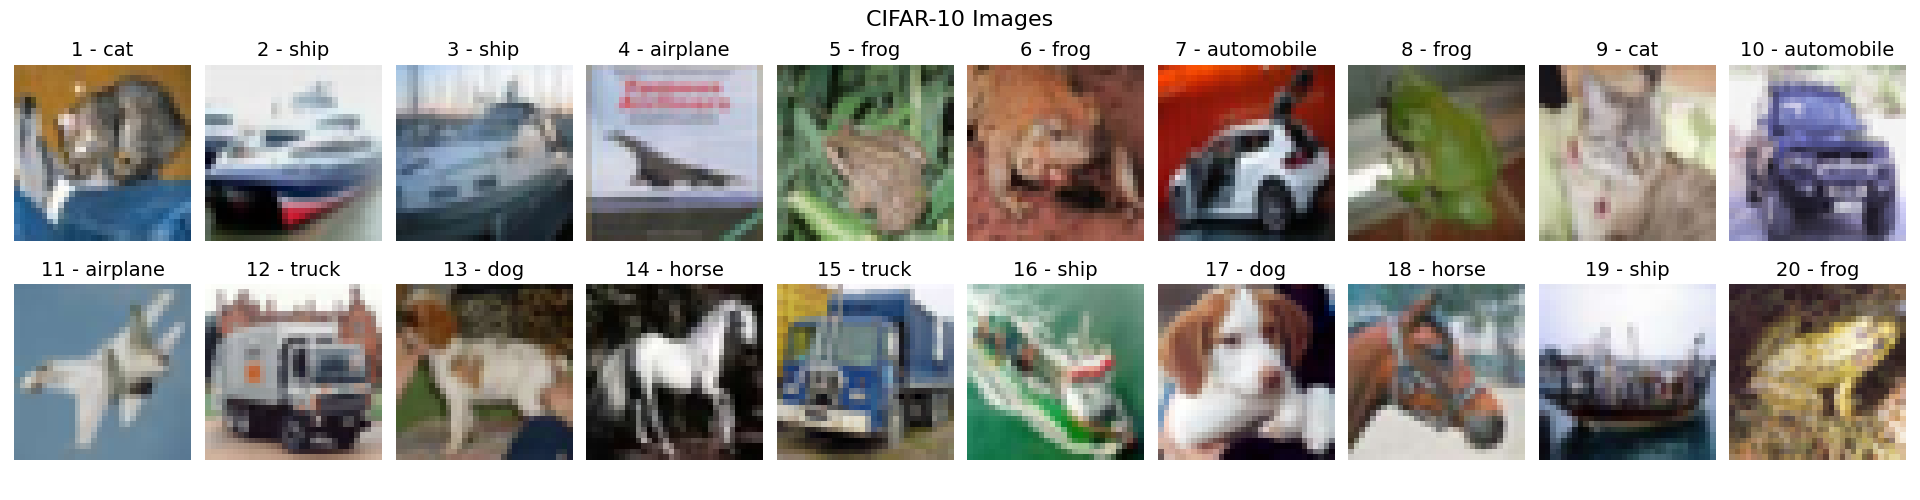
\includegraphics[width=0.99\textwidth]{Figures/Methods/CIFAR-10-Images-20imgs-2rows-10cols.png}
\caption{Examples of the CIFAR-10 dataset classes.}
\label{fig:Images-20imgs-2rows-10cols}
\end{figure}

The MNIST dataset (\cite{mnist}) is a collection of 70,000 (60k training, 10k testing) grayscale handwritten digit images (0-9), widely used for image classification benchmarking. It comprises 60,000 training images and 10,000 test images, each 28x28 pixels and is widely used for testing machine learning models. CIFAR-10 (\cite{cifar10}) consists of 60,000 (50k training, 10k testing) colour images (32x32 pixels) across 10 classes, like airplanes, cats, and trucks as shown in Figure \ref{fig:Images-20imgs-2rows-10cols}. It has 50,000 training images and 10,000 test images. 

%%%%%%%%%%%%%%%%%%%%%%%%%%%%%%%%%%%%%%%
% DATASETS VARIANTS AND PERTURBATIONS %
%%%%%%%%%%%%%%%%%%%%%%%%%%%%%%%%%%%%%%%

\subsection{Dataset Variants}

%%%%%%%%%%%%%%%%%%%%%%%
% MNISTIFIED DATASETS %
%%%%%%%%%%%%%%%%%%%%%%%

%\textbf{"MNISTified" Datasets}

\begin{figure}[h]
\centering
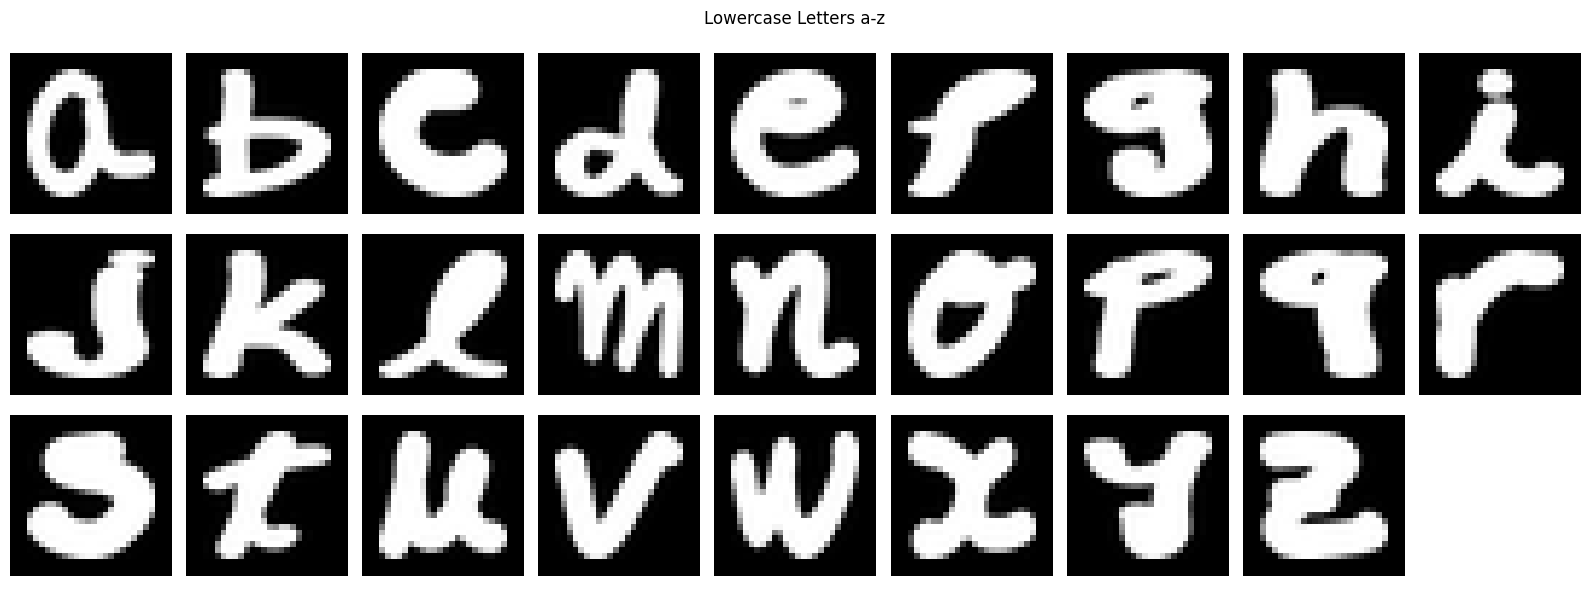
\includegraphics[width=0.99\textwidth]{Figures/Results/HandwrittenCharacters/mnistified-a-z.png}
\caption{Example of the MNISTified English handwritten lower case alphabetical characters.}
\label{fig:mnistified-a-z-methods}
\end{figure}

\textbf{MNISTified English Handwritten Characters - Digits and Alphabetical Characters} dataset \cite{deCampos09} subjects a CNN trained on MNIST to broader character sets. The base dataset contains 3,410 images of handwritten English characters across 62 classes: digits 0-9, uppercase A-Z, and lowercase a-z as shown in Figure \ref{fig:mnistified-a-z-methods}, with 55 images per class.
Images were preprocessed to match MNIST format: inverted to white characters on black backgrounds, resized to 28×28 pixels, and trimmed to remove excess margins. This preprocessing enables direct application of MNIST-trained models to character data.
The datasets test model performance across distribution shifts. The digits subset provides near-distribution evaluation, containing the same character types as MNIST training data. The alphabetical subset introduces varying degrees of out-of-distribution challenge, from characters visually similar to digits (Z resembles 2, upper case B resembles 8, lowercase b resembles 6) to completely dissimilar characters with no digit-like features.
This progression from in-distribution digits to out-of-distribution alphabetical characters allows systematic evaluation of how distance-based safety measures respond to increasing distribution shift.

\textbf{MNISTified CIFAR-10} converts CIFAR-10 color images to 28×28 grayscale format, matching MNIST dimensions.

%%%%%%%%%%%%%%%%%%%%%%%%%%%%%%%%%%%%%%%%
% THE PERTURBED MNIST (PMNIST) DATASET %
%%%%%%%%%%%%%%%%%%%%%%%%%%%%%%%%%%%%%%%%

%\subsubsection{The Perturbed MNIST (PMNIST) Dataset}

\begin{figure}[h]
\centering
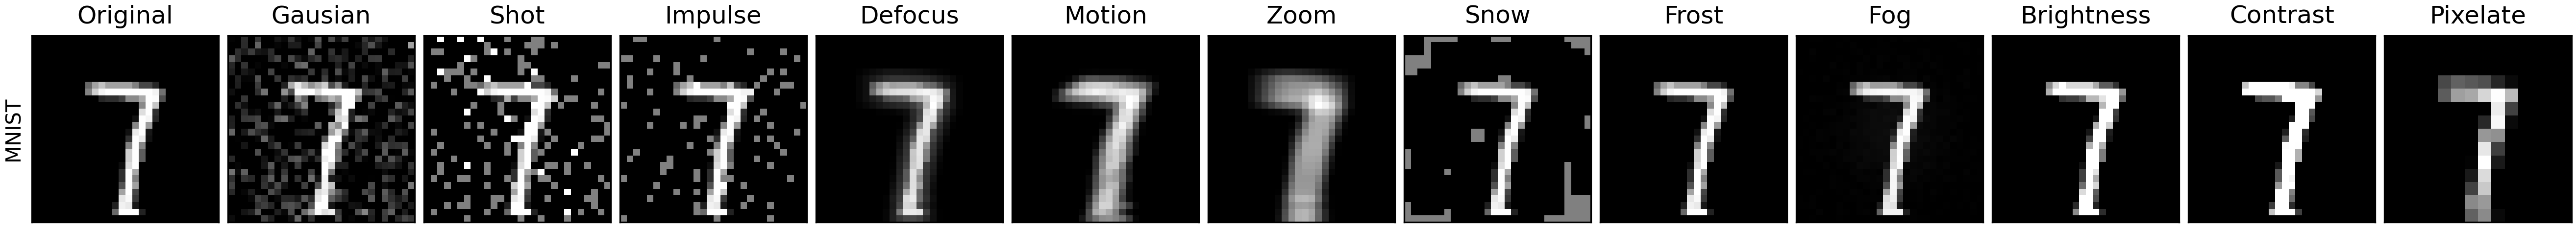
\includegraphics[width=0.99\textwidth]{Figures/Methods/MNIST_Perturbations.png}
\caption{Examples of the Perturbed MNIST - PMNIST dataset.}
\label{fig:MNIST_Perturbations}
\end{figure}

The Perturbed MNIST dataset (Figure \ref{fig:MNIST_Perturbations}) is an extension of the MNIST dataset and was created during the course of this study, to analyse the effect of noise on a neural network classifier's predictive accuracy. The MNIST dataset is a well known benchmark for evaluating the performance of algorithms in the Computer Vision domain. Comprising a collection of 70,000 grayscale images, each of 28x28 pixel resolution, the dataset is divided into two sets: a training set containing 60,000 examples, and a test set with 10,000 examples (\cite{lecun1998gradient}). Each image within the dataset is associated with a label from 0 to 9, the class index corresponding to the digit it represents.

A key feature of the MNIST dataset is its pre-processing stage, where the digits have been size-normalized and centered in a fixed-size image. This pre-processing reduces the variability unrelated to digit identity, allowing researchers to focus on the algorithmic challenge of digit recognition rather than on the preprocessing steps.

% The significance of the MNIST dataset in the realm of machine learning research is well-documented, with \cite{lecun1998gradient} providing an extensive overview of the dataset's creation, characteristics, and its role in fostering advancements in the field.

% This foundational dataset has contributed to the proliferation of research in neural networks, serving as a pivotal benchmark for innovations in the field of computer vision.

% Dataset description %

\textbf{MNIST structure description}: To extend the MNIST dataset it is necessary to understand its structure. The MNIST dataset is comprised of two main components: image files and label files, structured as follows:

\begin{itemize}
    \item \textbf{Training Set Images:} Contains 60,000 training examples.
    \item \textbf{Test Set Images:} Contains 10,000 test examples.
    \item Each image is encoded as a 28x28 pixel grid, summing up to 784 pixels per image. Each pixel represents a grayscale intensity, where 0 and 255 denote black and white respectively.
\end{itemize}

The image file is constructed with the following sequence of bytes:
\begin{enumerate}
    \item \textbf{Magic Number:} The first 4 bytes signify a magic number (2051) that identifies the file format.
    \item \textbf{Number of Images:} The following 4 bytes denote the count of images, encoded as a 32-bit integer.
    \item \textbf{Rows:} The subsequent 4 bytes illustrate the number of rows (28) per image, encoded as a 32-bit integer.
    \item \textbf{Columns:} The next 4 bytes depict the number of columns (28) per image, encoded as a 32-bit integer.
    \item \textbf{Pixel Values:} The remainder of the file is populated with pixel values in row-major order, with each image delineated sequentially in the file. Each pixel value is stored as an unsigned byte, representing the pixel's intensity.
\end{enumerate}

and label files:

\begin{itemize}
    \item \textbf{Training Set Labels:} Comprises 60,000 labels corresponding to the training images.
    \item \textbf{Test Set Labels:} Comprises 10,000 labels corresponding to the test images.
    \item Each label is a single byte signifying the digit (0 through 9) that the corresponding image represents.
\end{itemize}

The structure of the label files is detailed next:
\begin{enumerate}
    \item \textbf{Magic Number:} The first 4 bytes signify a magic number (2049) that identifies the file format.
    \item \textbf{Number of Items:} The following 4 bytes denote the count of labels, encoded as a 32-bit integer.
    \item \textbf{Labels:} The remainder of the file contains label values, stored as unsigned bytes, with each label corresponding to the image of the same index in the image file.
\end{enumerate}

Adhering to the standardized format ensures the modified MNIST dataset's compatibility with existing codebases.

\begin{table}[h]
\centering
\begin{tabular}{|l|l|r|r|}
\hline
\textbf{Type}             & \textbf{File Name}                       & \textbf{Size (B)} & \textbf{Count} \\ \hline
Training Images & \texttt{train-images-idx3-ubyte} & 47040016           & 60000 \\
Training Labels & \texttt{train-labels-idx1-ubyte} & 60008             & 60000 \\
Testing Images  & \texttt{t10k-images-idx3-ubyte}  & 7840016           & 10000 \\
Testing Labels  & \texttt{t10k-labels-idx1-ubyte}  & 10008              & 10000 \\ \hline
\end{tabular}
\caption{MNIST Dataset Files, file sizes in bytes and image/label count}
\label{table:mnist_files_b}
\end{table}
The contents can be examined with the \textit{xxd} command:
\begin{verbatim}
!xxd -C 'data/MNIST/raw/train-images-idx3-ubyte' | head

00000000: 0000 0803 0000 ea60 0000 001c 0000 001c  .......`........
00000010: 0000 0000 0000 0000 0000 0000 0000 0000  ................
00000020: 0000 0000 0000 0000 0000 0000 0000 0000  ................
00000030: 0000 0000 0000 0000 0000 0000 0000 0000  ................
00000040: 0000 0000 0000 0000 0000 0000 0000 0000  ................
00000050: 0000 0000 0000 0000 0000 0000 0000 0000  ................
00000060: 0000 0000 0000 0000 0000 0000 0000 0000  ................
00000070: 0000 0000 0000 0000 0000 0000 0000 0000  ................
00000080: 0000 0000 0000 0000 0000 0000 0000 0000  ................
00000090: 0000 0000 0000 0000 0000 0000 0000 0000  ................

!xxd -C 'data/MNIST/raw/train-labels-idx1-ubyte' | head

00000000: 0000 0801 0000 ea60 0500 0401 0902 0103  .......`........
00000010: 0104 0305 0306 0107 0208 0609 0400 0901  ................
00000020: 0102 0403 0207 0308 0609 0005 0600 0706  ................
00000030: 0108 0709 0309 0805 0903 0300 0704 0908  ................
00000040: 0009 0401 0404 0600 0405 0601 0000 0107  ................
00000050: 0106 0300 0201 0107 0900 0206 0708 0309  ................
00000060: 0004 0607 0406 0800 0708 0301 0507 0107  ................
00000070: 0101 0603 0002 0903 0101 0004 0902 0000  ................
00000080: 0200 0207 0108 0604 0106 0304 0509 0103  ................
00000090: 0308 0504 0707 0402 0805 0806 0703 0406  ................
\end{verbatim}

% Sanity check - number of files ~ 7260000 
% hex(7260000)
% '0x6ec760'
% int('006ec760', 16)
% 7260000 ~ pmnist training dataset
% int('001339e0', 16)
% 1260000 ~ pmnist testing dataset

% xxd perturbed-train-images-idx3-ubyte
% 00000000: 0000 0803 006e c760 0000 001c 0000 001c  .....n.`........
% xxd perturbed-train-labels-idx1-ubyte
% 00000000: 0000 0801 006e c760                      .....n.`
% xxd perturbation-train-levels-idx0-ubyte
% 00000000: 0000 07ff 006e c760                      .....n.`
% xxd t1260k-perturbed-images-idx3-ubyte
% 00000000: 0000 0803 0013 39e0 0000 001c 0000 001c  ......9.........
% xxd t1260k-perturbed-labels-idx1-ubyte
% 00000000: 0000 0801 0013 39e0                      ......9.
% xxd t1260k-perturbation-levels-idx0-ubyte
% 00000000: 0000 07ff 0013 39e0                      ......9.

Where hex \textbf{0000 0803} is the magic number 2051 (images), and hex \textbf{0000 0801} is the magic number 2049 (labels), hex \textbf{0000 ea60}, 60,000 decimal, is the number of examples in the dataset, and hex \textbf{0000 001c}, decimal 28, is the number of rows, and columns, in every image. Therefore the number of bytes in train-images-idx3-ubyte is $4 * 4 + 60000 * 28 * 28 = 47,040,016$.

The first image in the training dataset can be obtained by offsetting the first 16 bytes (magic number, number of images, row size and column size) and taking the next 784 bytes, then splitting the array into 28 rows.


\begin{figure}[h]
    \centering
    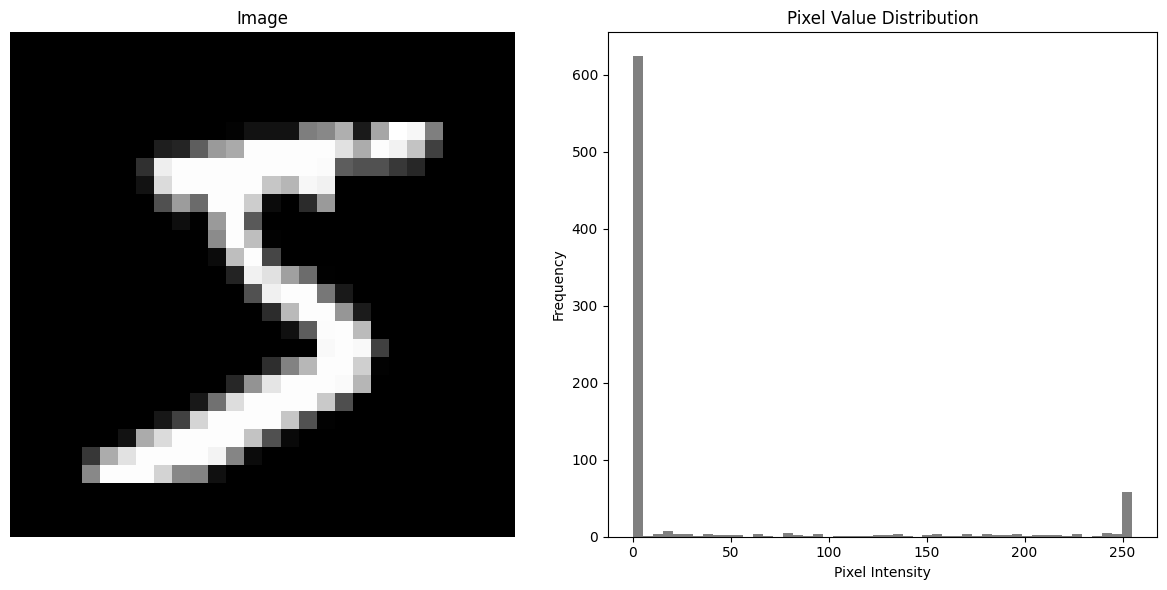
\includegraphics[width=0.75\textwidth]{Figures/Methods/MNIST_5_with_histogram.png}
    \caption{The first image in the MNIST training dataset; digit 5 and its pixel value distribution histogram scaled to 0-255 pixel intensity values.}
    \label{fig:mnist_5_histogram}
\end{figure}
As shown in Figure~\ref{fig:mnist_5_histogram}, the MNIST digit 5 is displayed alongside its pixel value distribution histogram where the pixel values range from 0 to 255. Figure~\ref{fig:mnist_0_histogram} shows the second image (zero) in the MNIST training dataset.

\begin{figure}[h]
    \centering
    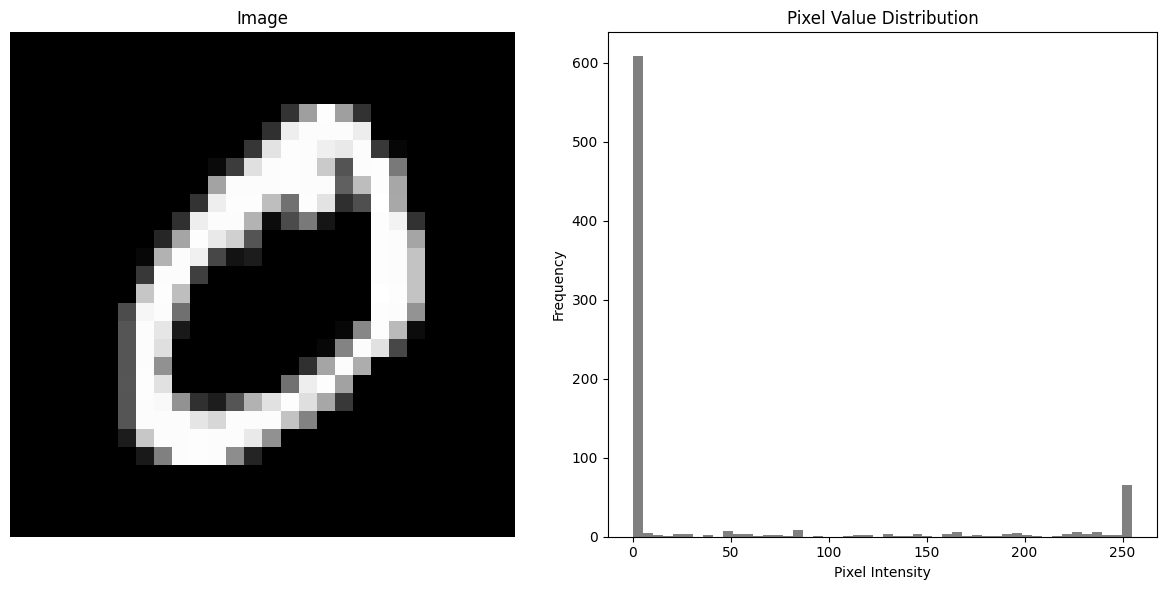
\includegraphics[width=0.75\textwidth]{Figures/Methods/MNIST_0_with_histogram.png}
    \caption{The second digit in the MNIST training dataset; digit 0 and its pixel value distribution histogram.}
    \label{fig:mnist_0_histogram}
\end{figure}

From the training labels dataset, it can be seen that by offsetting the magic number and the number of labels, represented by 4 bytes each, the following bytes represent the labels, that is, the first two labels are "05 and "00", matching figures \ref{fig:mnist_5_histogram} and \ref{fig:mnist_0_histogram}.

%%%%%%%%%%%%%%%%%%%%%%%%%%%%%%%%%%%%%
% CREATING THE NOISY PMNIST DATASET %
%%%%%%%%%%%%%%%%%%%%%%%%%%%%%%%%%%%%%

\textbf{Creating the "perturbed" PMNIST dataset}: The perturbed dataset incorporates a variety of perturbations to the original images, aiming to simulate real-world conditions where image data may not be ideal. Specifically, we introduce noise to the images using 12 distinct functions, designed to add noise, categorized as follows:

\begin{enumerate}
    \item \textbf{Pixel Intensity Adjustment:}
    \begin{itemize}
        \item Brightness
        \item Contrast
    \end{itemize}
    \item \textbf{Blurring:}
    \begin{itemize}
        \item Defocus Blur
        \item Motion Blur
        \item Zoom Blur
    \end{itemize}
    \item \textbf{Noise:}
    \begin{itemize}
        \item Gaussian Noise
        \item Impulse Noise
        \item Shot Noise
    \end{itemize}
    \item \textbf{Weather:}
    \begin{itemize}
        \item Fog
        \item Frost
        \item Snow
    \end{itemize}
    \item \textbf{Special Effects:}
    \begin{itemize}
        \item Pixelation
    \end{itemize}
\end{enumerate}

Each image in the original testing dataset undergoes a transformation by all perturbation methods, resulting in a companion image that retains the original label but exhibits the added noise or effect. The new dataset consist of the clean (original) and the noisy (perturbed) versions. 
%**TODO, describe new method storing perturbation and level in lower and upper nibbles.**
To distinguish and subsequent analysis, labels will be appended to denote the image type: "0xFF" for clean/original images and "01" for noisy/perturbed images. This dual dataset structure will enable comprehensive evaluation of machine learning models' performance in recognizing digits under varied noise regimes.
%, thereby enhancing the robustness of our image recognition pipeline.

% Applying noise

To generate our new dataset, images are appended to a binary file named perturbed-train-images-idx3-ubyte, where the first 16 bytes are:
\begin{verbatim}
0000 0803 0001 d4c0 0000 001c 0000 001c    
\end{verbatim}
Where 0001 d4c0 hex is 120000 decimal, the size of the new training dataset, twice the size of the original dataset.

A random selection of a perturbation type is made, and a perturbation level ranging from 0 to 9, and apply the perturbation to the image.

Figures \ref{fig:MNIST_4_clean_with_histogram} and \ref{fig:MNIST_4_noisy_with_histogram} show digit 4 with no noise and zoom blur level 8 applied.
\begin{figure}[h]
    \centering
    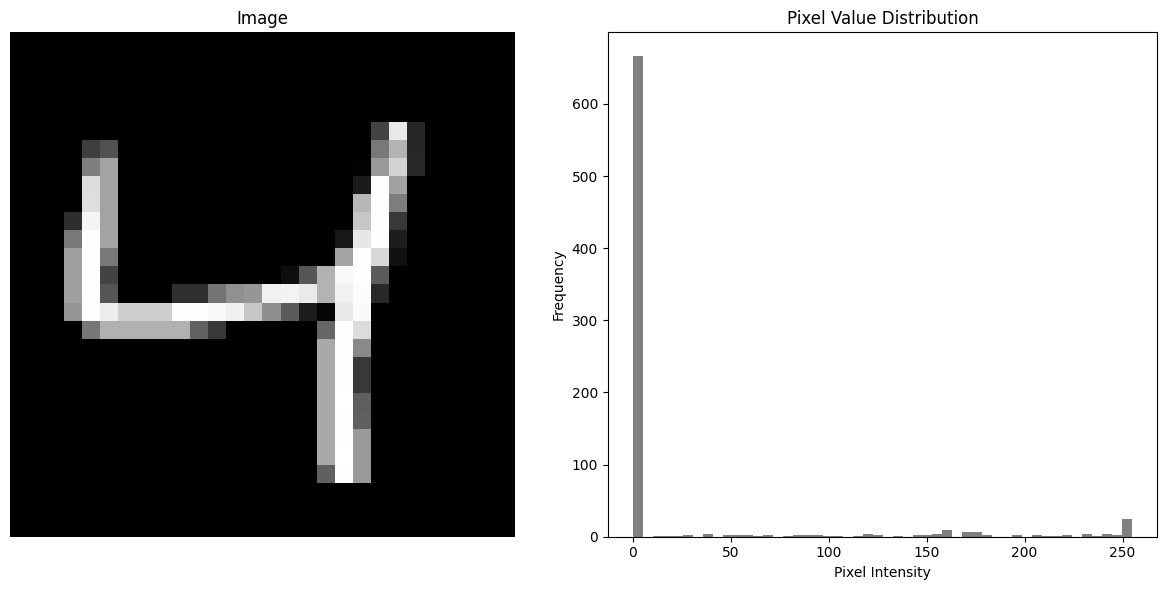
\includegraphics[width=0.75\textwidth]{Figures/Methods/MNIST_4_clean_with_histogram.png}
    \caption{MNIST digit 4 with no noise.}
    \label{fig:MNIST_4_clean_with_histogram}
\end{figure}

\begin{figure}[h]
    \centering
    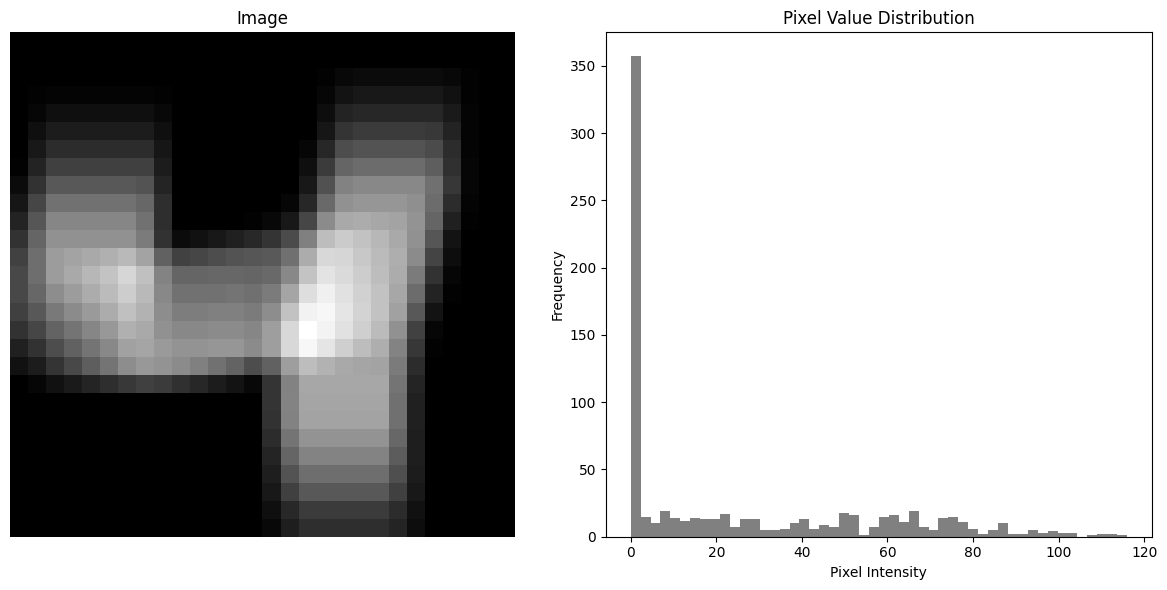
\includegraphics[width=0.75\textwidth]{Figures/Methods/MNIST_4_noisy_with_histogram.png}
    \caption{MNIST digit 4 with Zoom Blur level 8.}
    \label{fig:MNIST_4_noisy_with_histogram}
\end{figure}

% file to generate images is
% https://colab.research.google.com/drive/1s-KBSwUtT7tp280iLi8KgyHk4zThDnKD#scrollTo=OMq-a-wuKqR0
% MNIST-Dataset.ipynb

The process can be described as:

\begin{lstlisting}[caption={MNIST Perturbation Algorithm}, label={lst:mnist_perturbation_algorithm}]
Function createFiles():
    Open images.bin as binary write
    Open labels.bin as binary write
    Open perturbations.bin as binary write

Function saveImage(image, file):
    Write image to file

Function saveLabel(label, file):
    Write label to file as a single byte

Function savePerturbation(perturbationCode, file):
    Write perturbationCode to file as bytes

Function main():
    createFiles()
    For each image in MNIST:
        saveImage(originalImage, images.bin)
        saveLabel(0x00, labels.bin)
        savePerturbation(0xFFFF, perturbations.bin)
        
        perturbedImage = applyRandomPerturbation(originalImage)
        saveImage(perturbedImage, images.bin)
        saveLabel(0x01, labels.bin)
        perturbationCode = getPerturbationCode()
        savePerturbation(perturbationCode, perturbations.bin)

\end{lstlisting}

The same process is applied to training and testing datasets, and end up with 6 files, training and testing, 3 testing files are shown in Table \ref{table:mnist_perturbed_files_b}.

% \begin{table}[h]
% \centering
% \begin{tabular}{|l|l|r|r|}
% \hline
% \textbf{Type}             & \textbf{File Name}                          & \textbf{Size (B)} & \textbf{Count} \\ \hline
% Perturbed Training Images  & \texttt{perturbed-train-images-idx3-ubyte}    & TBA               & 120000 \\                            
% Perturbed Training Labels  & \texttt{perturbed-train-labels-idx1-ubyte}    & TBA               & 120000 \\                            
% Perturbation Training Levels  & \texttt{perturbation-train-levels-idx0-ubyte} & TBA               & 120000 \\
% Perturbed Testing Images   & \texttt{t20k-perturbed-images-idx3-ubyte}     & TBA               & 20000 \\                            
% Perturbed Testing Labels   & \texttt{t20k-perturbed-labels-idx1-ubyte}     & TBA               & 20000 \\  
% Perturbation Testing Levels   & \texttt{t20k-perturbation-levels-idx0-ubyte}     & TBA               & 20000 \\ \hline                 
% \end{tabular}
% \caption{Perturbed MNIST (PMNIST) Dataset Files, file sizes in bytes and image/label count}
% \label{table:mnist_perturbed_files_b}
% \end{table}

\begin{table}[h]
\centering
{\small
\begin{tabular}{|l|l|l|r|r|}
\hline
\textbf{ID} & \textbf{Type}                   & \textbf{File Name}                                   & \textbf{Size (M)} & \textbf{Count} \\ \hline
% 1 & Perturbed Training Images       & \texttt{perturbed-train-images-idx3-ubyte}    & TBA               & 7260000 \\
% 2 & Perturbed Training Labels       & \texttt{perturbed-train-labels-idx1-ubyte}    & TBA               & 7260000 \\
% 3 & Perturbation Training Levels    & \texttt{perturbation-train-levels-idx0-ubyte} & TBA               & 7260000 \\
1 & Perturbed Testing Images        & \texttt{t1210k-perturbed-images-idx3-ubyte}     & 905M               & 1210000 \\
2 & Perturbed Testing Labels        & \texttt{t1210k-perturbed-labels-idx1-ubyte}     & 1.2M               & 1210000 \\
3 & Perturbation Testing Levels     & \texttt{t1210k-perturbation-levels-idx0-ubyte}  & 1.2M               & 1210000 \\ \hline
\end{tabular}
} % End of \small
\caption{Perturbed MNIST (PMNIST) Dataset Files, file sizes in bytes and image/label count}
\label{table:mnist_perturbed_files_b}
\end{table}

Where the additional files are perturbation-train-levels-idx0-ubyte and t20k-perturbation-levels-idx0-ubyte that contain the perturbation types and levels, stored contiguously in one byte values. As per the algorithm listed in Listing \ref{lst:mnist_perturbation_algorithm}, We start by opening the binary files. We then iterate over every image in the MNIST dataset. We apply a random perturbation and perturbation level to the image, writing the original and perturbed image to the new PMNIST dataset (ID 1). We write the image label twice (ID 2), once with value 0 indicating the image is noise-free, and once with value 1 indicating the image is perturbed, aligning with the saved images and finally we write the perturbation key and level (ID 3). We repeat the steps for the testing dataset, obtaining 3 additional files (IDs 4, 5 and 6).

%%%%%%%%%%%%%%%%%%%%%%%%%%%%%%
% NOISE PERTURBATION METHODS %
%%%%%%%%%%%%%%%%%%%%%%%%%%%%%%

%\subsubsection{Noise Perturbation Methods}
%\label{methods:noise_perturbation}

Twelve distinct noise perturbation types are applied to MNIST training images to simulate real-world degradation conditions and evaluate model robustness, based on \cite{hendrycks2019benchmarking}. Each perturbation type operates across ten intensity levels designed to produce approximately-linear accuracy degradation from near 100\% accuracy (level 0) to average 50\% (level 10). All perturbations operate on grayscale images with pixel values normalized to the range $[-1, 1]$.

Parameter values for each perturbation type and intensity level were determined through trial-and-error, adjusting parameters until the linear degradation profile was approximated.

The twelve perturbation types are:

\textbf{Brightness} adjusts global illumination by adding constant values ranging from 0.1 to 1.0 across intensity levels. Higher values simulate overexposure conditions.

\textbf{Contrast} modifies pixel intensity relationships relative to the image mean. Positive values (3.0 to 0.2) increase contrast while negative values (-0.2 to -0.6) reduce contrast, simulating poor lighting conditions.

\textbf{Defocus Blur} applies uniform convolution kernels of varying sizes (3×3 to 8×8) with blur amounts from 0.1 to 1.5, simulating camera focus issues.

\textbf{Fog} creates atmospheric scattering effects using Gaussian distance-based masks with fog levels and densities ranging from 0.1 to 0.6, simulating reduced visibility conditions.

\textbf{Frost} generates crystalline patterns through thresholded Gaussian noise (levels 6 to 18) followed by Gaussian blurring with 5×5 kernels, simulating ice formation on camera lenses.

\textbf{Gaussian Noise} adds normally distributed random values with means from 0.05 to 0.87 and fixed standard deviation of 0.25, simulating sensor thermal noise.

\textbf{Impulse Noise} introduces salt-and-pepper artifacts by randomly setting pixel values to maximum intensity, with density ranging from 0.25 to 0.75, simulating sensor dead pixels.

\textbf{Motion Blur} applies directional convolution kernels of increasing size (1×1 to 10×10) at 0° angle, simulating camera or subject movement.

\begin{figure}[h]
\centering

\includegraphics[width=0.99\textwidth]{Figures/Methods/Pixelation_Digit_5_1_to_10_intensity.png}
\caption{MNIST Digit 5 subject to 10 levels of pixelation from left to right.}
\label{fig:Pixelation_Digit_5_1_to_10_intensity}
\end{figure}

\textbf{Pixelation} (Figure \ref{fig:Pixelation_Digit_5_1_to_10_intensity}) reduces spatial resolution through downsampling by factors from 0.7 to 5.7 followed by nearest-neighbor upsampling, simulating low-resolution capture conditions.

\textbf{Shot Noise} introduces Poisson-distributed noise with intensities from 0.1 to 0.57, simulating photon counting limitations in low-light conditions.

\textbf{Snow} creates precipitation effects by randomly placing high-intensity pixels (snow levels 0.81 to 0.99) followed by Gaussian blurring, simulating weather-related occlusion.

\textbf{Zoom Blur} applies radial blur kernels of increasing size (1×1 to 8×8) with unit strength, simulating rapid focal length changes or camera shake.

All perturbation implementations use OpenCV (\cite{opencv}) for image processing operations.

%%%%%%%%%%%%%%%%%%%%%%%
% MODEL ARCHITECTURES %
%%%%%%%%%%%%%%%%%%%%%%%

\section{Model Architectures}

%%%%%%%%%%%%%%%%%%%%%%%%%%%%%%%%
% NEURAL NETWORK ARCHITECTURES %
%%%%%%%%%%%%%%%%%%%%%%%%%%%%%%%%

\subsection{Convolutional Neural Networks (CNNs)} 

CNNs process images through hierarchical feature extraction (\cite{lecun1998gradient}). Convolutional layers apply learnable filters across input images to generate feature maps detecting edges, textures, and objects. ReLU activation introduces non-linearity. Pooling layers downsample feature maps for computational efficiency and translation invariance. Fully connected layers perform final classification using extracted high-level features.

\subsection{Vision Transformers (ViTs)} 
ViTs treat images as sequences of fixed-size patches (\cite{dosovitskiy2021image}). Each patch is flattened and embedded into vector space with positional encodings preserving spatial relationships. A classification token aggregates global image representation. Multi-head self-attention mechanisms enable each patch to attend to all others, capturing long-range dependencies. Feed-forward networks process attention outputs before final classification.

\subsection{Vision-Language Models (VLMs)} 
VLMs integrate visual and textual processing through specialized architectures. Qwen-VL combines a ViT visual encoder with the Qwen LLM backbone (\cite{bai2023qwen}). A position-aware cross-attention adapter compresses visual features from 1024+ tokens to 256 fixed-length representations for efficient LLM processing. DeepSeek-VL employs hybrid vision encoding: SigLIP-L processes low-resolution semantic features while SAM-B captures high-resolution details \cite{zeng2024deepseek}. A two-layer MLP adapter fuses these representations into 576 visual tokens for the DeepSeek-LLM backbone.

%%%%%%%%%%%%%%%%%%%%%%%%%%%%%%%%%%
% MODEL TRAINING AND FINE-TUNING %
%%%%%%%%%%%%%%%%%%%%%%%%%%%%%%%%%%

\section{Model Training and Fine-Tuning}

%%%%%%%%%%%%%%%%
% CNN TRAINING %
%%%%%%%%%%%%%%%%

\subsection{CNN Training}
Images undergo three preprocessing steps before CNN input. Vertical cropping removes sky and hood regions, retaining pixels from y-coordinate 210 to 480. Spatial downsampling resizes cropped images to 200×66 pixels using bilinear interpolation. Color space conversion transforms RGB to YUV \cite{lecun2004dave, bojarski2016end} In the RGB scheme, each pixel is represented by three channel intensities of red, green and blue. In YUV, also referred to as YCbCr (\cite{maller2020}) space, each pixel is represented by Y (luma), U (Cb - luminance value subtracted from red channel) and V (Cr - luminance value subtracted from red channel). It is a "lossy" process which degrades the data, and originally developed for colour to black and white television backward compatibility. Moving the image from RGB to YUV space has been demonstrated to give "better subjective image quality than the RGB color space", being better for computer vision "implementations than RGB due to the perceptual similarities to the human vision" (\cite{podpora2014yuv}). No data augmentation is applied. 

The CNN implements the NVIDIA architecture from Bojarski et al. (2016) \cite{bojarski2016end} with standard regression and modifications for classification outputs. Five convolutional layers use ELU activation with kernel sizes [5,5,5,3,3] and strides [2,2,2,1,1]. Channel progression follows [24,32,48,64,64]. Four fully connected layers with dimensions [1152,100,50,10] precede the output layer. Dropout with probability 0.1 follows each layer. Input normalization divides pixel values by 255.

Training uses an 80/20 random train-validation split with shuffled indices. Adam optimizer applies learning rate 1e-5 with default momentum parameters. Cross-entropy loss trains classification variants; mean squared error trains regression variants. Batch size is 64 samples. Training runs for maximum 100 epochs with early stopping monitoring validation loss. Early stopping triggers after 6 epochs without improvement, restoring the best model state. Training executes on NVIDIA GPU with CUDA acceleration. Best-performing models save as PyTorch state dictionaries including model weights, optimizer state, epoch number, and final loss values.

%%%%%%%%%%%%%%%%%%%%%%%%%%%%%%%%
% VIT TRAINING AND FINE-TUNING %
%%%%%%%%%%%%%%%%%%%%%%%%%%%%%%%%

\subsection{ViT Training and Fine-Tuning}

\textbf{ViT Training}
\label{methods:vit_from_scratch}
Vision Transformers train from scratch using patch-based image tokenization. Images are divided into non-overlapping patches of size 8×8 pixels for CIFAR-10 and 4×4 pixels for MNIST. Each patch is flattened and linearly projected to embedding dimension 64. Positional embeddings are added to patch embeddings before input to the transformer encoder.

The transformer architecture uses 6 encoder layers with 4 attention heads per layer. Each encoder layer contains multi-head self-attention followed by a feed-forward network with expansion factor 2. Dropout probability is 0.1 for all layers. Layer normalization applies before attention and feed-forward blocks following the pre-norm configuration.

Training uses Adam optimizer with peak learning rate 5e-4 and 10-epoch linear warmup. Batch size is 128 samples. Training runs for 5000 epochs without early stopping. RandAugment data augmentation applies during training with default parameters. Training executes on GPU when available with automatic fallback to CPU. Model checkpoints save based on configurable frequency, with final models stored as complete state dictionaries.

\textbf{ViT Fine-tuning:} Pre-trained Vision Transformer fine-tuning adapts Google's ViT-base-patch16-224 (\cite{google2021vitbasepatch16224}) weights for both regression and classification tasks. Models initialize with ImageNet weights. Classification heads modify original 1000-class outputs to task-specific dimensions: single output for regression, N outputs for N-class classification.
Image preprocessing standardizes inputs to 224×224 pixel resolution for both variants. Dataset creation extracts steering angle labels from CARLA image metadata. Images convert to RGB format before processing. Dataset splits use 80/20 random train-validation division.
Training applies identical configurations across task types. Batch size sets to 16 samples per device for training and evaluation. Learning rate uses 2e-5 with 30 training epochs. Evaluation runs per epoch with matching save frequency.
Loss functions differ by task: mean squared error for regression variants, cross-entropy loss for classification variants. Regression evaluation computes MAE and MSE. Classification evaluation computes accuracy from predicted classes. Best model selection uses task-appropriate metrics: MAE minimization for regression, accuracy maximization for classification.
Model checkpointing saves every 500 steps with maximum three checkpoints retained. Training logs save to timestamped directories with automatic visualization. Final models save as complete directories containing weights, configuration, and preprocessing parameters.

%%%%%%%%%%%%%%%%%%%%%%%%%%%%%%%%%%%%%
% VISION-LANGUAGE MODEL FINE-TUNING %
%%%%%%%%%%%%%%%%%%%%%%%%%%%%%%%%%%%%%
% For results, see experiments 269 onwards

\subsection{VLM Fine-Tuning}
Vision-language model fine-tuning adapts Qwen2-VL-2B-Instruct (\cite{bai2023qwen}) for steering decision tasks using supervised fine-tuning with conversational data. The base model initializes with pre-trained multimodal weights supporting both vision and language understanding.

Dataset preparation extracts steering angles from CARLA image filenames and maps binned  values to verbal directional commands. Three steering bins define the classification space: 0.0000 maps to "Straight", -0.0650 maps to "Left", and 0.0650 maps to "Right". Each sample pairs CARLA simulator images with a fixed query prompt "What direction the vehicle should be steering?" and corresponding directional labels.

Training data structures as three-role conversations following chat template formatting. System messages define the model as a steering specialist constrained to output only directional commands. User messages combine CARLA images with steering queries. Assistant messages provide single-word directional responses matching the three-class label space.

Fine-tuning applies QLoRA (\cite{dettmers2023qlora}) parameter-efficient training targeting query and value projection layers. LoRA \cite{hu2021lora} configuration uses rank 8 with alpha 16 and 5\% dropout. Training runs for 3 epochs with batch size 4 per device and gradient accumulation over 8 steps. Learning rate sets to 2e-4 with constant scheduling and 3\% warmup ratio.
Loss computation applies standard causal language modeling with special handling for vision tokens. Image token embeddings exclude from loss calculation to focus learning on text generation. Gradient checkpointing enables training within memory constraints while maintaining bfloat16 precision throughout.

Model checkpointing saves every 20 steps with evaluation-based selection using validation loss minimization. Final models save as complete directories containing adapted weights, tokenizer configuration, and image processor settings.

%%%%%%%%%%%%%%%%%%%%%%%%%%%%%%%%%%%
% EVALUATION AND ANALYSIS METHODS %
%%%%%%%%%%%%%%%%%%%%%%%%%%%%%%%%%%%

\section{Evaluation and Analysis Methods}

Network evaluation can be categorized into two cases: where the CARLA simulator is required, and where it is not. In the latter case, the dataset (whether for self-driving regression or classification, or CIFAR-10, MNIST and MNISTified datasets) can be accessed in a single inference loop and is not subject to the constraints described next.

Network evaluation for real-time self-driving operates under constraints imposed by CARLA simulator compatibility requirements. CARLA 0.9.13 requires Python 3.6.9 for API wrapper functionality, while the transformers libraries require Python 3.11.0 or greater. Two different evaluation schemes addressed in the following subsections are used to address the issue.

%%%%%%%%%%%%%%%%%%%%%%%%%%%%%%%%%%%%%%%%%%%%%%%%%%%%%%%%%%%%%%%%%%%%
% NETWORK EVALUATION SETUPS (SINGLE, DUAL, AND REMOTE ENVIRONMENTS %
%%%%%%%%%%%%%%%%%%%%%%%%%%%%%%%%%%%%%%%%%%%%%%%%%%%%%%%%%%%%%%%%%%%%

\subsection{Network Evaluation Setups (Single, Dual, and Remote Environments)}

\textbf{CNN Single-Environment Evaluation:} CNN evaluation (no transformers model required) runs entirely within Python 3.6.9 environment. CARLA simulation and CNN inference execute in the same environment space, enabling direct model integration within the simulation loop.

\textbf{ViT/VLM Dual-Environment Evaluation:}
\begin{figure}[h]
\centering
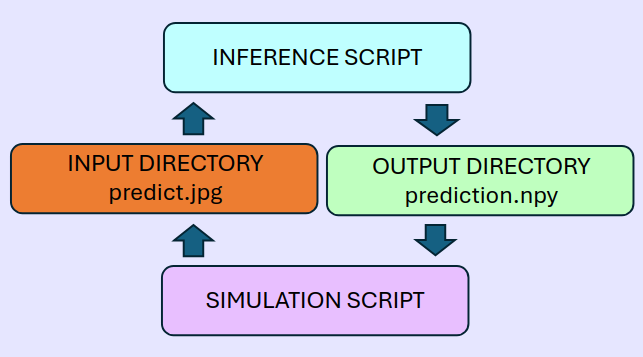
\includegraphics[width=0.50\textwidth]{Figures/Methods/LocalVLMInference.png}
\caption{Local ViT/VLM inference workflow, where a simulation script generates an output image predict.jpg taken from vehicle's front facing camera and the inference script generates a softmax output predict.npy that the simulation script collects to then extract the steering angle that should be applied to the simulated vehicle.}
\label{fig:LocalVLMInference}
\end{figure}

As previously mentioned, ViT (as well as VLM) evaluation requires separate Python environments. CARLA simulation is controlled in a Python 3.6.9 environment while ViT inference runs in a Python 3.11.0 environment. Inter-process communication bridges the two environments, transferring image data from simulation to inference process and returning steering predictions. This architecture introduces additional latency through disk-based communication. Images write to disk from CARLA simulation and read from disk by ViT inference process. Predictions write to disk by ViT inference as plain text files containing single float steering angles for regression tasks or as pickle files containing softmax outputs for classification tasks. CARLA simulation subsequently reads prediction files from disk. The simulation process takes care of reading the prediction file, then deleting the prediction file and writing an image file to disk e.g. predict.jpg . The inference process takes care of reading the image, then deleting the image and writing the inference file to disk e.g. prediction.npy. The flow (excluding file deletions) is shown in Figure \ref{fig:LocalVLMInference}.

\begin{figure}[h]
\centering
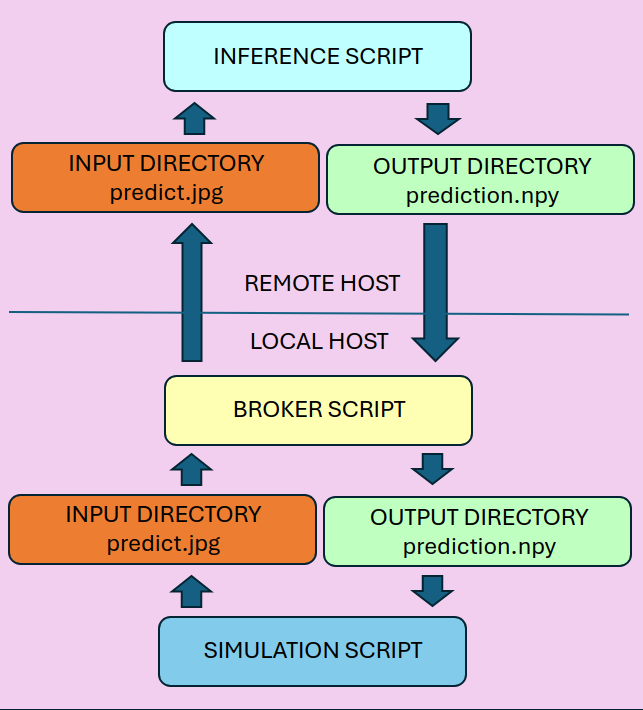
\includegraphics[width=0.50\textwidth]{Figures/Methods/RemoteVLMInference.png}
\caption{Remote VLM inference workflow, where a simulation script generates an output image predict.jpg taken from vehicle's front facing camera, the broker script transfers to the remote host, the inference script generates a softmax output predict.npy that the broker transfers to local host, finally simulation script collects to then extract the steering angle that should be applied to the simulated vehicle.}
\label{fig:RemoteVLMInference}
\end{figure}

% \begin{verbatim}                                    
% +-------------------------------------+
% |           INFERENCE SCRIPT          |
% +-----------------------------+-------+
%          ^                    |       
%          |                    v       
% +-----------------+ +------------------+
% | INPUT DIRECTORY | | OUTPUT DIRECTORY |
% | predict.jpg     | | prediction.npy   |
% +-----------------+ +--------+---------+
%          ^                    |       
%          |                    v       
% +-------------------------------------+
% |         SIMULATION SCRIPT           |     
% +-------------------------------------+
% \end{verbatim}


\textbf{VLM Remote Evaluation:} VLM evaluation addresses memory constraints through remote inference deployment. The local workstation does not have enough GPU memory to run Qwen2-VL model inference at the same time, so the inference is run on the HPC cluster. Image and prediction file exchange occurs in the same way as with the local dual-environment, with the addition of a broker process that takes care to transfer files from local to remote filesystems and back again, while also dealing with file deletions. The flow is described in Figure \ref{fig:RemoteVLMInference}. 

% \begin{verbatim}
% +-------------------------------------+
% |           INFERENCE SCRIPT          |
% +-----------------------------+-------+
%          ^                    |       
%          |                    v       
% +---------+-------+ +------------------+
% | INPUT DIRECTORY | | OUTPUT DIRECTORY |
% | predict.jpg     | | prediction.npy   |
% +-----------------+ +--------+---------+
%          ^   REMOTE HOST     |       
% ---------+--------------------+--------
%          |   LOCAL HOST      |       
% +---------+--------------------+-------+
% |           BROKER SCRIPT             |
% +--------+--------------------+-------+
%          |                    |       
%          |                    v       
% +---------+--------+ +------------------+
% | INPUT DIRECTORY | | OUTPUT DIRECTORY |
% | predict.jpg     | | prediction.npy   |
% +-----------------+ +--------+---------+
%          ^                    |       
%          |                    v       
% +-------------------------------------+
% |         SIMULATION SCRIPT           |
% +-------------------------------------+
% \end{verbatim}   

% \ref{app_res:290}.

%%%%%%%%%%%%%%%%%%%%%%%%%%%%%%%%%%%%%%%%%%
% REGRESSION-TO-CLASSIFICATION TRANSFORM %
%%%%%%%%%%%%%%%%%%%%%%%%%%%%%%%%%%%%%%%%%%

\subsection{Regression-to-Classification Transformation}
\label{methods:regression_classification}

To apply the method described in Section \ref{methods:clustering} to the self-driving steering-angle prediction problem, it is necessary to transform neural network regressors as seen in end-to-end learning approaches for autonomous driving (\cite{lecun2004dave,bojarski2016end}), into classifiers. The output layer was modified from one neuron producing a single continuous value to $N$ neurons corresponding to $N$ discrete bins classes. The final linear transformation changed from a mapping to $\mathbb{R}^1$ to a mapping to $\mathbb{R}^N$, where $N$ represents the number of steering angle bins (3, 5, or 15). 

The problem of selecting the number of bins when discretising continuous variables has been studied in the statistical literature on histogram construction. Classical approaches include Sturges’ rule (\cite{sturges1926}), Scott’s rule (\cite{scott1979}), and the Freedman–Diaconis rule (\cite{freedman1981}), while more recent work has proposed Bayesian and penalised-likelihood methods (\cite{knuth2006,birge2006}). These methods show that the optimal binning depends on sample size, data spread, and the intended task. The choice of bin numbers was determined empirically in this study, with 3 and 5 bins found to provide the best performance for steering classification, Sturge's, Scott's and Freedman-Diaconis suggest 16, 52 and 67 bins respectively, for 28k examples which is the typically size of the training dataset for self-driving.

The regression model outputs a single value interpreted directly as the predicted steering angle. The classification model outputs $N$ logits passed through softmax activation to produce binned steering angle class probabilities, where each class represents a steering angle. The number of bins must always be odd such that the middle bin corresponds to zero degree (straight) steering.

Loss functions changed from Mean Squared Error (MSE) for regression to Cross-Entropy Loss for classification. Evaluation metrics changed from Mean Absolute Error (MAE) to classification accuracy, calculated as the percentage of images where the predicted class matches the true class. Training procedures remained otherwise identical, including learning rates, batch sizes, and early stopping criteria (\cite{goodfellow2016deep}).

%%%%%%%%%%%%%%%%%%%%%%%%%%%%%%%%%%%%%%%%%%%%%%%%%%%%%%%%%%%%%%%
% UNCERTAINTY QUANTIFICATION VIA SOFTMAX CLUSTERING ALGORITHM %
%%%%%%%%%%%%%%%%%%%%%%%%%%%%%%%%%%%%%%%%%%%%%%%%%%%%%%%%%%%%%%%

\subsection{Uncertainty Quantification via Softmax Clustering}
\label{methods:clustering}

\sloppy

We consider a neural network output vector $\mathbf{p} = (p_1, p_2, \dots, p_K)$ where $\sum p_i = 1$, representing a probability distribution obtained by normalizing the logit vector $\mathbf{z} = (z_1, z_2, \dots, z_K)$ through the softmax function, $p_i = \text{softmax}(z_i) = e^{z_i} / \sum_{j=1}^{K} e^{z_j}$. For example, given $\mathbf{p} = [0.01, 0.01, 0.01, 0.01, 0.9, 0.01, 0.01, 0.01, 0.01, 0.01]$, the predicted class is '4', corresponding to the highest value at index five, reflecting the confidence of the prediction for each class from '0' to '9'. The logits, representing log-likelihoods of class memberships, are related to probabilities by $z_i = \log (p_i / (1 - p_i))$ where $z_i$ is the logit for class $i$, and $p_i$ is the probability of the input belonging to class $i$.
%\cite{goodfellow2016deep,bishop2006pattern}.

We store the predictions for MNIST and CIFAR-10 datasets in a matrix $\mathbf{M} \in \mathbb{R}^{n \times 12}$, where $n$ is the number of predictions, the first ten columns are the softmax probabilities, column 11 is the true class and column 12 is the predicted class.
To obtain cluster centroids $\mathbf{C} \in \mathbb{R}^{10 \times 10}$ we calculate the mean of all correct predictions from the training datasets with Algorithm \ref{alg:k-means-centroid-init}. To calculate the softmax distance threshold we use all incorrect predictions with Algorithm \ref{alg:min_distance}.

\begin{algorithm}
\caption{K-Means Centroid Initialisation from Softmax Outputs}
\label{alg:k-means-centroid-init} 
\begin{algorithmic}[1]
\Require{$correct\_preds$: array of shape $(n, 12)$, where $n$ is the number of correct predictions}
\Ensure{$centroids$: array of shape $(10, 10)$, initialised centroids for each digit class}

\State $probs\_dist \gets correct\_preds[:, :10]$ \Comment{Extract probability distribution for each digit}
\State $centroids \gets \text{zeros}((10, 10))$ \Comment{Initialise centroids array}

\For{$digit \gets 0$ to $9$}
\State $indices \gets \text{where}(\text{argmax}(probs\_dist, \text{axis}=1) == digit)[0]$ \Comment{Find indices of rows where digit has highest probability}
\State $centroid \gets \text{mean}(probs\_dist[indices], \text{axis}=0)$ \Comment{Compute mean probability distribution for selected rows}
\State $centroids[digit] \gets centroid$ \Comment{Assign centroid to corresponding row in centroids array}
\EndFor

\State \textbf{return} $centroids$
\end{algorithmic}
\end{algorithm}

%%%%%%%%%%%%%%%%%%%%%%%%%%%%%
% GEOMETRIC CHARACTERISTICS %
%%%%%%%%%%%%%%%%%%%%%%%%%%%%%

\textbf{Geometric Characteristics of Probability-Constrained Cluster Spaces}: Cluster centroids produced by  softmax layer outputs adhere to valid probability distributions. This requires each coordinate \( c_i \) to satisfy \( 0 \leq c_i \leq 1 \) and the sum \( \sum_{i=1}^n c_i = 1 \), confining the centroids to the vertices and interior of the standard \((n-1)\)-dimensional simplex. For two such centroids \( \mathbf{c}_1 \) and \( \mathbf{c}_2 \) within the \( n \)-dimensional unit hypercube under these constraints, the Euclidean distance between centroids \( \mathbf{c}_1, \mathbf{c}_2 \in [0,1]^n \) is \( d(\mathbf{c}_1, \mathbf{c}_2) = \sqrt{\sum_{i=1}^{n}\left(c_{1i} - c_{2i}\right)^2} \). When enforcing probabilistic constraints via softmax normalization, the maximum achievable distance between centroids remains bounded by \(\sqrt{2}\), independent of the dimensionality \( n \).

\begin{algorithm}
\caption{Find Minimum Softmax Distances to Centroids for Incorrectly Predicted Digits (Threshold)}
\label{alg:min_distance} 
\begin{algorithmic}[1]
\Procedure{FindMinDistances}{$data$}
    \State $labels \gets [0, 1, 2, 3, 4, 5, 6, 7, 8, 9]$
    \State $thresh \gets \text{empty array of shape } (10, 2)$
    \For{$i \gets 0 \text{ to } 9$}
        \State $label \gets labels[i]$
        \State $min\_dist \gets \min(data[data[:, 1] == label, 0])$
        \State $thresh[i, 0] \gets min\_dist$
        \State $thresh[i, 1] \gets label$
    \EndFor
    \State \textbf{return} $thresh$
\EndProcedure
\end{algorithmic}
\end{algorithm}

\textbf{Cluster Density}: Quantifying cluster density in high-dimensional softmax spaces provides insight into the confidence of neural network predictions. The density of a cluster in an $n$-dimensional space is quantified using the following equations:
\begin{equation}
\rho_k = \frac{N_k}{V_n(r_k)}, \quad V_n(r_k) = \frac{\pi^{n/2}}{\Gamma\left(\frac{n}{2} + 1\right)} r_k^n, \quad N_k = \sum_{i=1}^n \mathbf{1}(\|\mathbf{x}_i - \mathbf{c}\| \leq r_k) \label{eq:density_volume_count}
\end{equation}

\noindent where \(\rho_k\) is the cluster density for radius scaling factor \(k\) \cite{ester1996density}, \(N_k\) is the number of points within radius \(r_k\), \(V_n(r_k)\) is the volume of the \(n\)-dimensional hypersphere with radius \(r_k\) \cite{Conway1998}, \(r_k = k \cdot r\) is the scaled radius, \(k\) is the scaling factor, \(r\) is the base radius, \(n\) is the number of dimensions, \(\pi\) is the mathematical constant, \(\Gamma\) is the gamma function, \(\mathbf{1}\) is the indicator function, \(\mathbf{x}_i\) is the \(i\)-th point’s coordinates, \(\mathbf{c}\) is the cluster centroid, and \(\|\cdot\|\) is the Euclidean norm, measuring the distance between points \cite{Duda2000}. These enable evaluation of cluster compactness at varying radii \cite{Hastie2009}.

The volume $V_{shell}$ of a shell between inner and outer radii $r_1, r_2$  is given by:

\begin{equation}
V_{\text{shell}}(n, r_1, r_2) = \frac{\pi^{n/2}}{\Gamma(n/2 + 1)} \cdot \left( r_2^n - r_1^n \right)
\end{equation}

The number of points $N_{shell}$ in a shell is given by $ N_{shell}(r_1,r_2) = N_{r_2} - N_{r_1} $, where $N_{r_2}$ is the number of points within a hypersphere of radius $r_2$ and $N_{r_1}$ is the number of points within hypersphere of radius $r_1$, where both hyperspheres are concentric and $r_2 > r_1$.

In n-dimensional spaces, hypersphere shells demonstrate volume distribution patterns that differ significantly from low-dimensional intuition. For n > 5, the volume concentrates predominantly in outer shells, while exponentially decreasing toward the center. The ratio between consecutive shell volumes increases with dimension, creating a steep volume gradient. This concentration effect stems from the $r^n$ term in the above volume formula. This affects nearest-neighbor calculations and creates challenges for clustering algorithms with most points existing near the hypersphere's surface rather than distributed throughout its volume. To handle this issue, in our approach thresholds will be calculated w.r.t. the true and predicted classes in the training set.

%%%%%%%%%%%%%%%%%%%%%%%%%%%%%%%%%%%
% DISTANCE METRICS: BD, HI and KL %
%%%%%%%%%%%%%%%%%%%%%%%%%%%%%%%%%%%

\subsection{Image Distance Metrics}
\label{methods:distance_metrics}

Three statistical distance metrics are employed to quantify distances between original and noise-corrupted images: Bhattacharyya Distance, Histogram Intersection, and Kullback-Leibler (KL) Divergence. 

The Bhattacharyya Distance (\cite{bhattacharyya1943}) is a statistical measure used to quantify the similarity between two probability distributions. It provides a way to measure the amount of overlap between two statistical samples or populations, indicating how "close" they are to each other in a statistical sense.

Histogram Intersection (\cite{swain1991}) is a method used in computer vision to compare the similarity of two images. It operates by measuring the overlap between two colour histograms, effectively counting the number of pixels from a model that have corresponding pixels of the same colour in a target image. 

The Kullback-Leibler Divergence (\cite{kullback1951}) is a measure from information theory that quantifies how one probability distribution differs from a second, reference distribution. It is used to calculate the information lost when an approximate model is used to represent a true distribution, effectively measuring their dissimilarity. 

Standard formulations are adapted for multi-channel RGB images by computing histogram-based representations for each colour channel. Bhattacharyya Distance and KL Divergence increase as dissimilarity increases, while Histogram Intersection decreases as dissimilarity increases.

For RGB images treated as histogram distributions with ground truth and corrupted bin counts $P,Q$ respectively, the total pixel count is:
\begin{equation}
\label{eq:t_p}
  t_p = \prod\limits_{n=1}^{N}I_n   
\end{equation}
where $N$ is the number of image dimensions and $I_n$ is the number of elements in dimension $n$.

\textbf{Bhattacharyya Distance} is defined as the negative logarithm of the Bhattacharyya coefficient:
\begin{equation}
    D_{B}(P,Q) = -\ln(BC(P,Q))
\end{equation}
where for multi-channel RGB:
\begin{equation}
BC(P,Q) = \sum\limits_{x\in \mathcal{X}} \frac{\sqrt{P(x)Q(x)}}{t_p}
\end{equation}

\textbf{Kullback-Leibler Divergence} for RGB images:
\begin{equation}
 D_{KL}(P \parallel Q) = \sum\limits_{x\in\mathcal{X}} \frac{P(x)}{t_p} \log\left(\frac{P(x)+\epsilon}{Q(x)+\epsilon}\right)
\end{equation}

We add a small positive term $ \epsilon $ to $ P(x), Q(x) $ to avoid division by zero, and also to avoid taking the logarithm base 10 of zero which is undefined.

We note that the KL Divergence in addition to, for our purposes, being fragile, is also asymmetric. that is the divergence from P to Q is not the same as the divergence from Q to P.

Note we use discrete rather than the continuous values. That is, we use the original byte value for each channel and the discrete relative entropy equation. If we convert the distribution to a PDF, that is, with all aggregated counts summing to one, we would use the continuous equation. The PDF seems like the better way to go as it is a normalised value, though if we are dealing with a known network, the input is always of the same the same dimensions and can be considered normative, that is the RGB mean is constrained by, and bound to, the input size.

\textbf{Histogram Intersection} for RGB distributions:
\begin{equation}
  H_{I}(P, Q) = \frac{1}{t_p} \sum\limits_{x\in\mathcal{X}}\min(P(x), Q(x))   
\end{equation}

If $P,Q$ are the same for every $ x $, then the summation will be equal to the product $t_p$, resulting in 1, meaning there is a complete overlap between the two distributions. If $argmin(P(x), Q(x))$ is equal to zero for every $x$, then the summation will be equal to zero meaning there is no overlap between the histograms.

Since the histogram RGB intersection does not take square roots or logs, it is the most computationally efficient of the three distance metrics we investigate.

%%%%%%%%%%%%%%%%%%%%%%%%%%%%
% ZERO-SHOT VLM EVALUATION %
%%%%%%%%%%%%%%%%%%%%%%%%%%%%

\subsection{Zero-Shot VLM Evaluation}

In addition to CNNs and ViTs, Vision Language Models (VLM) were also used for image classification (MNIST, CIFAR10) and self-driving, given that the VLM prediction is also a softmax output and therefore the methods developed in this study also apply. In the following subsections the models and tasks are described.

To gauge VLM scene understanding, the meta-llama/Llama-3.2-11B-Vision-Instruct (\cite{meta2024llama3vision}) model was evaluated on the CIFAR-10 dataset in a zero-shot setting where no pre-training and no image-query-reply examples are given to the model). This assessment measured the model's intrinsic visual understanding capabilities without any task-specific training or fine-tuning. The evaluation protocol involved presenting the model with CIFAR-10 images at three distinct input resolutions: standard 32x32, 720x720, and 1440x1440 pixels. 

The LLaMA-based Vision-Language Model (\cite{touvron2023llamaopenefficientfoundation}) \texttt{meta-llama/Llama-3.2-11B-Vision-Instruct} checkpoint was used to perform classification on CIFAR-10 images. The model integrates a vision encoder and a language generation head, allowing it to process images and produce textual class predictions within a unified architecture.

Input images were preprocessed differently across experiments to evaluate the impact of resolution on classification performance. One approach was to resize CIFAR-10 images from $32 \times 32$ pixels to $1440 \times 1440$ RGB images; another resized to $720 \times 720$ pixels; and a third approach passed images at their native resolution without resizing.

Each image was paired with a textual prompt listing the ten CIFAR-10 classes, effectively framing classification as a visual question answering task. The model’s textual output was parsed to extract predicted class names mapped back to CIFAR-10 labels.

The motivation is to evaluate how well a general-purpose Vision-Language Model (VLM), designed for broad multimodal tasks, can generalize effectively to standard benchmarks like CIFAR-10 without fine-tuning, compared to a ViT fine-tuned specifically on a given image dataset. For comparison, the Llama-3.2-11B-Vision-Instruct model has 11B parameters, while the ViT models used had between 500k to 100M parameters, where the standard  ViT model (\cite{dosovitskiy17}) has approximately 85M parameters.

\textbf{VLM Self-Driving Inference:} Vision-Language Models were adapted for steering prediction by constraining text generation to discrete steering classes. Three models were implemented: DeepSeek-VL-1.3B-Chat (\cite{zeng2024deepseek}) (local inference), Qwen2-VL-2B-Instruct (\cite{bai2023qwen}) (remote inference), and Grok-2-Vision-Latest (\cite{xai2025grok2vision}) (API-based inference). Each model processes front-facing CARLA camera images to generate categorical steering predictions. All models process CARLA images through multimodal interfaces with model-specific preprocessing requirements.

Prompts were crafted to elicit categorical responses such as  "Left, Straight or Right" or "Middle, Left, Right" rather than free-form text descriptions. Prompts were determined while aligning human scene understanding with the VLM understanding e.g. the VLMs tested did not understand the term "Lane Segmentation" so the segmentation was referred to as a "green patch" which the LLM could better identify on a scene.

Local and remote models provide direct access to token logits allowing full softmax distribution calculation across steering classes. API-based models return text responses only.


%% RESULTS
\chapter{Results}
\label{chap:results}

This chapter presents the experimental results obtained during the course of this study. A total of 285 experiments were documented across 290 experiment IDs, conducted between November 2021 and June 2025, spanning CARLA simulator setup, image classification, and autonomous driving model development.

Initial experiments (1-8) established the CARLA simulation environment with traffic generation, dynamic weather conditions, and vehicle control systems. Image classification experiments (11-28) systematically evaluated CNN accuracy degradation against 12 perturbation types on MNIST datasets, including development of a perturbed MNIST dataset for controlled noise analysis.

The research progressed through three phases. The early phase (experiments 1-50) focused on CNN baseline performance and simulation infrastructure development. The middle phase (experiments 51-150) introduced Vision Transformer architectures for image classification and autonomous driving, examining parameter scaling and pre-trained model adaptation. The advanced phase (experiments 151-290) incorporated Vision Language Models, applying multimodal architectures to the problem of steering prediction under noisy conditions.

Key experimental themes included noise impact analysis (47 experiments), infrastructure and hardware evaluation (13 experiments), and systematic comparison of CNN, ViT, and VLM architectures across multiple datasets. The methodology development progressed from image classification to regression-based steering prediction to classification-based approaches using discrete steering angle values discretized into bins. Autonomous driving experiments constituted approximately 70\% of the total research effort (201/285 experiments), with the CARLA simulator serving as the primary experimental platform. The experimental sequence shows progression from traditional computer vision approaches through convolutional models and transformer models to vision and multimodal large language models. The experiment logs are presented in a separate appendix.

The following sections present results organized according to the thesis objectives:

\begin{itemize}

\item Distance-based Distribution Shift Detection
\item Cross-architectural Validation on Standard Datasets
\item Accuracy Degradation Characterisation
\item Synthetic Dataset Creation for Autonomous Driving
\item Autonomous Driving Safety Application
\end{itemize}

\section{Datasets}

\begin{table}[ht]
\centering
\caption{Overview of Datasets. Abbreviations: 'reg' = regression dataset; 'seg' = lane segmentation present; 'fid' = fiducial markers present; 'bal' = balanced classes (minority classes duplicated); 'Img+Q+L' = image, query, and label formatted for Vision Language Models. Datasets 16 and 17 were generated at inference time and not saved to disk. Total images: 1,917,822.}
\label{tab:datasets}
\begin{tabular}{l l r l}
\toprule
\textbf{ID} & \textbf{Dataset Name} & \textbf{Count} & \textbf{Description} \\
\midrule
1 & PMNIST & 1,200,000 & Perturbed MNIST \\
2 & MNISTified CIFAR-10 & 50,000 & Grayscale CIFAR-10 \\
3 & MNISTified English Handwritten Digits & 550 & Conformed to MNIST\\
4 & MNISTified English Handwritten Characters & 2,860 & Conformed to MNIST\\
5 & carla\_dataset\_640x480\_01 & 29,105 & reg, seg with fid \\
6 & carla\_dataset\_640x480\_02 & 29,108 & reg, seg \\
7 & carla\_dataset\_640x480\_03 & 29,105 & reg, fid only \\
8 & carla\_dataset\_640x480\_05 & 29,013 & seg 15 bins \\
9 & carla\_dataset\_640x480\_05\_bal & 152,996 & seg 15 bins bal \\
10 & carla\_dataset\_640x480\_06 & 27,114 & seg, 5 bins \\
11 & carla\_dataset\_640x480\_06\_bal & 79,206 & seg 5 bins \\
12 & carla\_dataset\_640x480\_07\_3\_bins & 26,954 & seg 3 bins \\
13 & carla\_dataset\_640x480\_07\_3\_bins\_bal & 67,391 & seg 3 bins bal \\
14 & carla\_dataset\_640x480\_07\_3\_bins\_qwen & 26,950 & seg 3 bin Img+Q+L \\
15 & carla\_dataset\_640x480\_07\_3\_bins\_qwen\_bal & 67,380 & seg 3 bin Img+Q+L \\
16 & CIFAR-10 (zero-shot) & 50,000 & 1440x1440 px (not saved) \\
17 & CIFAR-10 (zero-shot) & 50,000 & 720x720 px (not saved) \\
\midrule
& \textbf{Total} & \textbf{1,917,822} & \\
\bottomrule
\end{tabular}
\end{table}

Table \ref{tab:datasets} shows datasets created for this project. MNIST variants (IDs 1-4), including PMNIST and MNISTified datasets, were created for image classification using CNN and ViT models. CARLA simulator-generated datasets (IDs 5-15) were created for autonomous driving testing, including CNN/ViT regression models and CNN/ViT classification models with quantized steering angles (3, 5, and 15 bins). Figure \ref{fig:mnistified_cifar10} shows examples of the MNISTified CIFAR-10 dataset.

\begin{figure}[h]
\centering
\includegraphics[width=0.99\textwidth]{Figures/Results/mnistified_cifar10.png}
\caption{Examples of the MNISTified CIFAR-10 dataset, where the RGB (three channel) images are converted to grayscale (single channel).}
\label{fig:mnistified_cifar10}
\end{figure}

For regression and classification models, the steering angle is embedded in the filename (e.g., \texttt{20250514\_154417\_678492\_steering\_0.0137.jpg}). The quantized steering angle datasets (3, 5, and 15 bins) use discrete values. For example, the 5-bin dataset uses values $-0.065$, $-0.015$, $0.000$, $0.015$, and $0.065$, corresponding to steering angles from $\pm$4.55 degrees, which is sufficient to navigate the figure-of-eight circuit in CARLA's Town04 map.

Datasets 14 and 15 extend datasets 12 and 13 by adding query prompts formatted for Vision Language Models. The system prompt instructs the model to act as a steering specialist and reply with only "Left", "Straight", or "Right" based on the provided image. The discrete steering angle labels ($-0.065$, $0.000$, $0.065$) were mapped to these natural language commands (Left, Straight, Right).

The VLM datasets (IDs 14 and 15) were used to fine-tune Qwen2-VL-2B-Instruct \cite{bai2023qwen} and deepseek-vl-1.3b-chat \cite{zeng2024deepseek} models. Datasets 16 and 17 were used for zero-shot evaluation with Llama-3.2-11B-Vision-Instruct \cite{meta2024llama3vision}.

\subsection{The Perturbed MNIST Dataset}

To characterise model prediction accuracy degradation as a function of added noise, we use a method similar to the work of \cite{hendrycks2019benchmarking}.

Through trial and error, parameter values were found for each perturbation function such that as the perturbation level increases from 1 to 10, the network predictive accuracy decreases from 98.52\% maximum to 36.32\% minimum, with average accuracy dropping from 97.61\% (level 1) to 48.83\% (level 10). The accuracy degradation can be observed in both Figures \ref{fig:Accuracy_vs_Noise_types} and \ref{fig:Pixelation_Digit_5_images_histogramsx10_plus_softmax}.

\begin{figure}[h!] 
\begin{center}
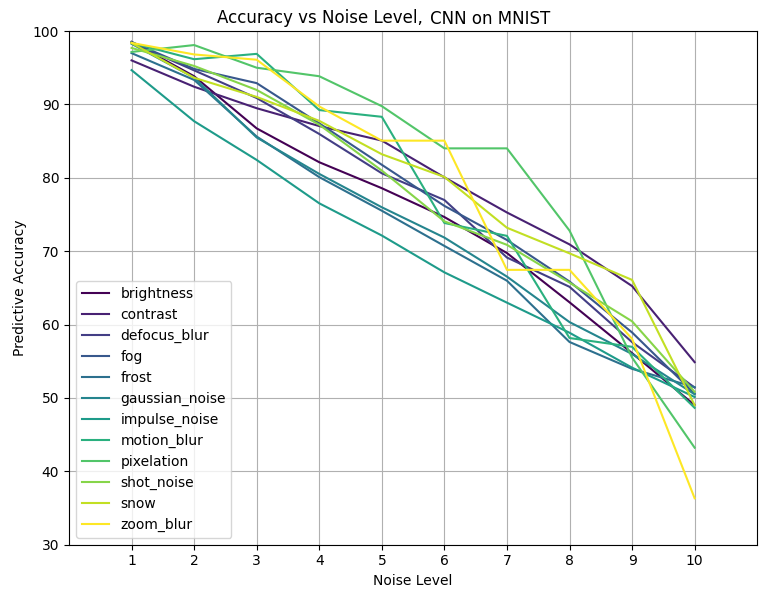
\includegraphics[width=0.99\columnwidth]{Figures/Results/Figures_accuracy_vs_noise_types_plot.png}
\end{center}
\caption{Plot for network accuracy degradation for individual perturbation types: Brightness, Contrast, Defocus Blur, Fog, Frost, Gaussian Noise, Impulse Noise, Motion Blur, Pixelation, Shot Noise, Snow and Zoom Blur.}
\label{fig:Accuracy_vs_Noise_types}
\end{figure}

Figure \ref{fig:Pixelation_Digit_5_images_histogramsx10_plus_softmax} shows digit class 5 subject to increasing levels of pixelation from left to right. The bottom row of the figure shows the average softmax output for all perturbation types at a given level. We note that at all levels from 1 to 10, the highest prediction is digit class 5 (sixth column from left to right on every plot, the first being for digit 0).
\begin{figure*}[h!]
    \centering
    
\includegraphics[width=0.99\textwidth]{Figures/Results/Figures_Pixelation_Digit_5_images_histogramsx10_plus_softmax.png}   %\captionsetup{justification=raggedright,singlelinecheck=false}
    \caption{Top row: MNIST class digit 5 subject 1 to 10 levels of pixelation going left to right. Bottom row: the average softmax output for the perturbed MNIST dataset class digit 5 for each perturbation level across all perturbation types. The change in bar heights is an indication of how images are moving closer and further to centroids in the cluster as noise increases.}\label{fig:Pixelation_Digit_5_images_histogramsx10_plus_softmax}
\end{figure*}

% generated with function call visualize_accuracy_heatmap(accuracy_matrix, perturbation_types, intensities)
\begin{figure*}[h!]
    \centering
    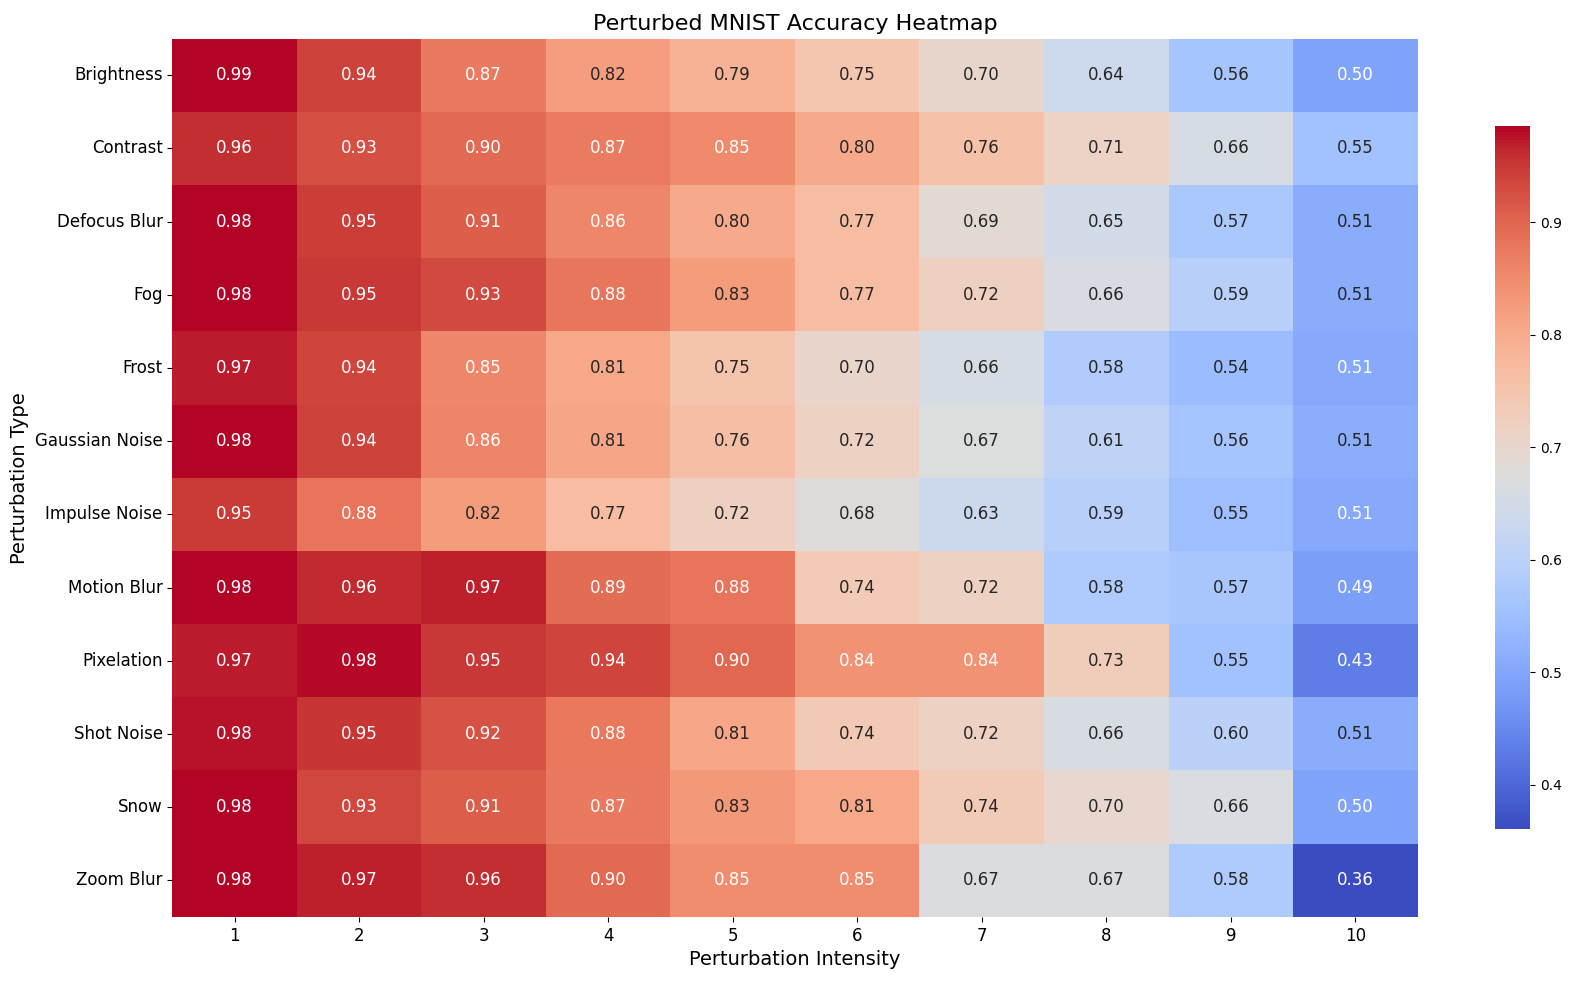
\includegraphics[width=0.99\textwidth]{Figures/Results/Figures_PerturbedMNISTAccuracyHeatmap.png}   %\captionsetup{justification=raggedright,singlelinecheck=false}
    \caption{Perturbed MNIST Accuracy Heatmap, where the accuracies are for all digit classes, given a perturbation type and intensity.}
    \label{fig:PerturbedMNISTAccuracyHeatmap}
\end{figure*}

Figure \ref{fig:PerturbedMNISTAccuracyHeatmap} shows a heatmap where every cell represents one perturbation type (y-axis, 12 total) at one intensity level (x-axis, 10 total) applied to the 10,000-image MNIST test dataset. The perturbed images are presented to the trained model and the resulting accuracy is placed in the corresponding cell. The heatmap therefore represents 1,200,000 predictions on perturbed images.

The heatmap uses a color scale from red to blue, with red indicating higher accuracy values and blue representing lower accuracy. As the perturbation intensity increases, the accuracy decreases for all perturbation types.

\begin{figure*}[h!]
    \centering
    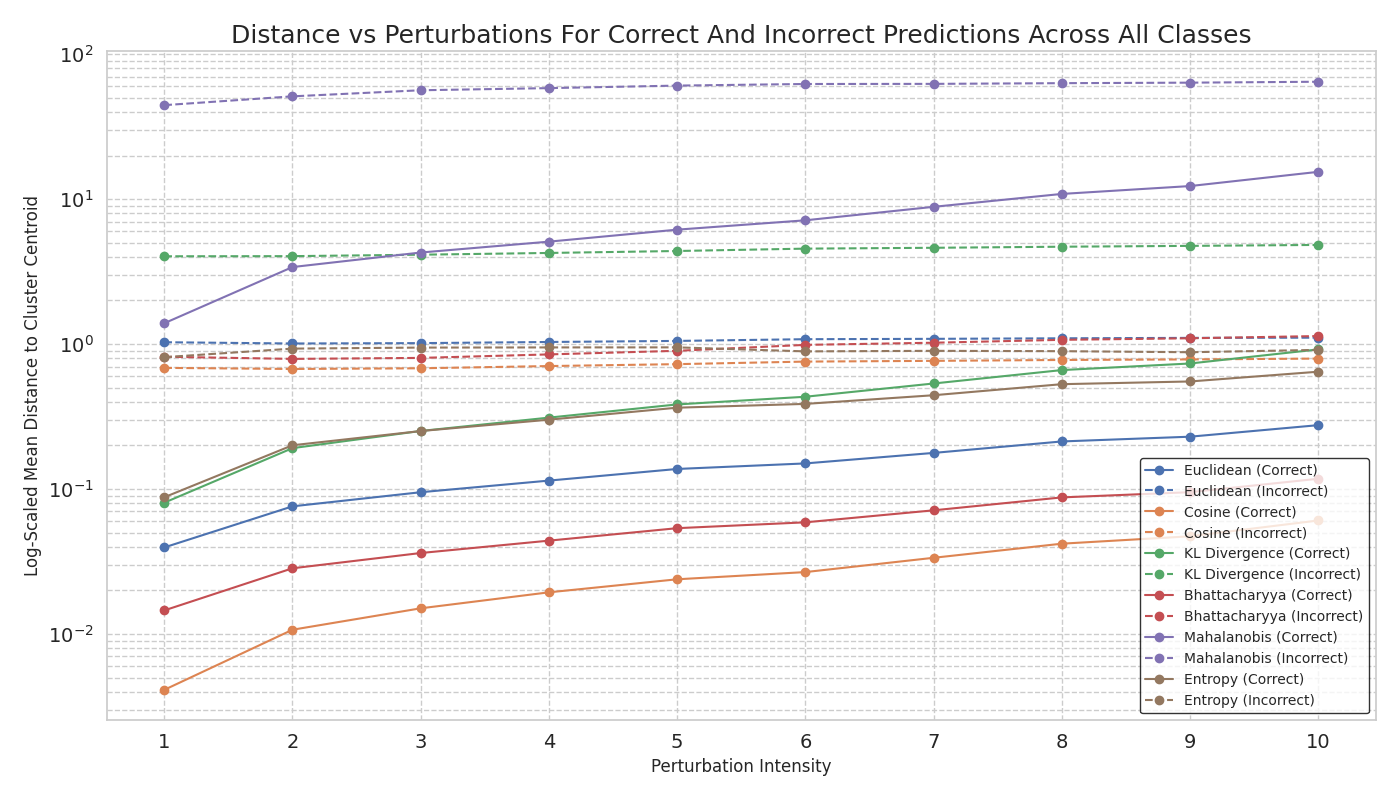
\includegraphics[width=0.99\textwidth]{Figures/Results/Figures_uncertainty_metrics.png}
    \caption{Comparison of correct vs. incorrect predictions across six distance metrics (log-scale). Solid lines represent correct predictions, dashed lines represent incorrect predictions.}
    \label{fig:Figures_uncertainty_metrics}
\end{figure*}

Figure \ref{fig:Figures_uncertainty_metrics} shows the average distance to class centroids across all classes and all perturbations for noise levels 1 through 10, comparing correct (solid line) and incorrect (dashed line) predictions for six distance metrics: Euclidean Distance, Cosine Similarity, KL Divergence, Bhattacharyya Distance, Mahalanobis Distance, and Entropy.

The plot shows that Cosine Similarity obtains maximum separation between correct and incorrect classifications, while Entropy obtains the minimum separation. Euclidean Distance proves not to be optimal; Cosine Similarity and Bhattacharyya Distance separate correct and incorrect classifications by nearly two orders of magnitude in low noise regimes and above one order of magnitude in high noise regimes, while Euclidean Distance separates by approximately one and a half orders of magnitude in low noise regimes and under one order of magnitude in high noise regimes.

The distance to centroids for correct predictions (solid lines) increases approximately linearly with perturbation intensity across all measures. The incorrect prediction distances (dashed lines) also increase with perturbation intensity but are less pronounced given the logarithmic y-axis scale. The separation between correct and incorrect predictions is important, as greater separation implies higher certainty in the decision space.

Most distance measures show good separation between correctly and incorrectly classified examples, with the exception being Entropy, which at the highest perturbation intensity presents the least separation. While Euclidean distance was selected for this study, these results suggest that alternative metrics, particularly Cosine Similarity, may provide better performance in future work.
%%%%%%%%%%%%%%%%%%%%%%%%%%%%%%%%%%%%%%%%%%
% SECTION ENGLISH HANDWRITTEN CHARACTERS %
%%%%%%%%%%%%%%%%%%%%%%%%%%%%%%%%%%%%%%%%%%

\subsection{MNISTified Datasets}

To establish a baseline for the geometric properties of the in-distribution data, we first characterized the average padding and centring of each digit in the original MNIST dataset. This provides a basis for conforming the out-of-distribution handwritten characters to a similar format.

This section describes the processes used to conform the English Handwritten Character Dataset \cite{deCampos09} to the MNIST dataset, to provide the model trained on the MNIST dataset, data that may be visually similar (digits) but not always related (characters) to the original MNIST dataset (digits)
The English Handwritten Characters Dataset  contains 3,410 images of handwritten characters in English, 62 classes and 55 images of each class: 0-9, A-Z and a-z. There are 1430 uppercase characters, 1430 lowercase characters and 550 digits. Image are 1200 x 900 pixels in size, all RGB (3 channel) in PNG format. Figure \ref{fig:sample_handwritten_characters} shows a sample of 12 characters. 

% Repo git@github.com:dsikar/work-in-progress.git
% Script exploratory-handwritten-digits-sample-2.py
% commit 11f=0b9af
\begin{figure}[ht]
    \centering
    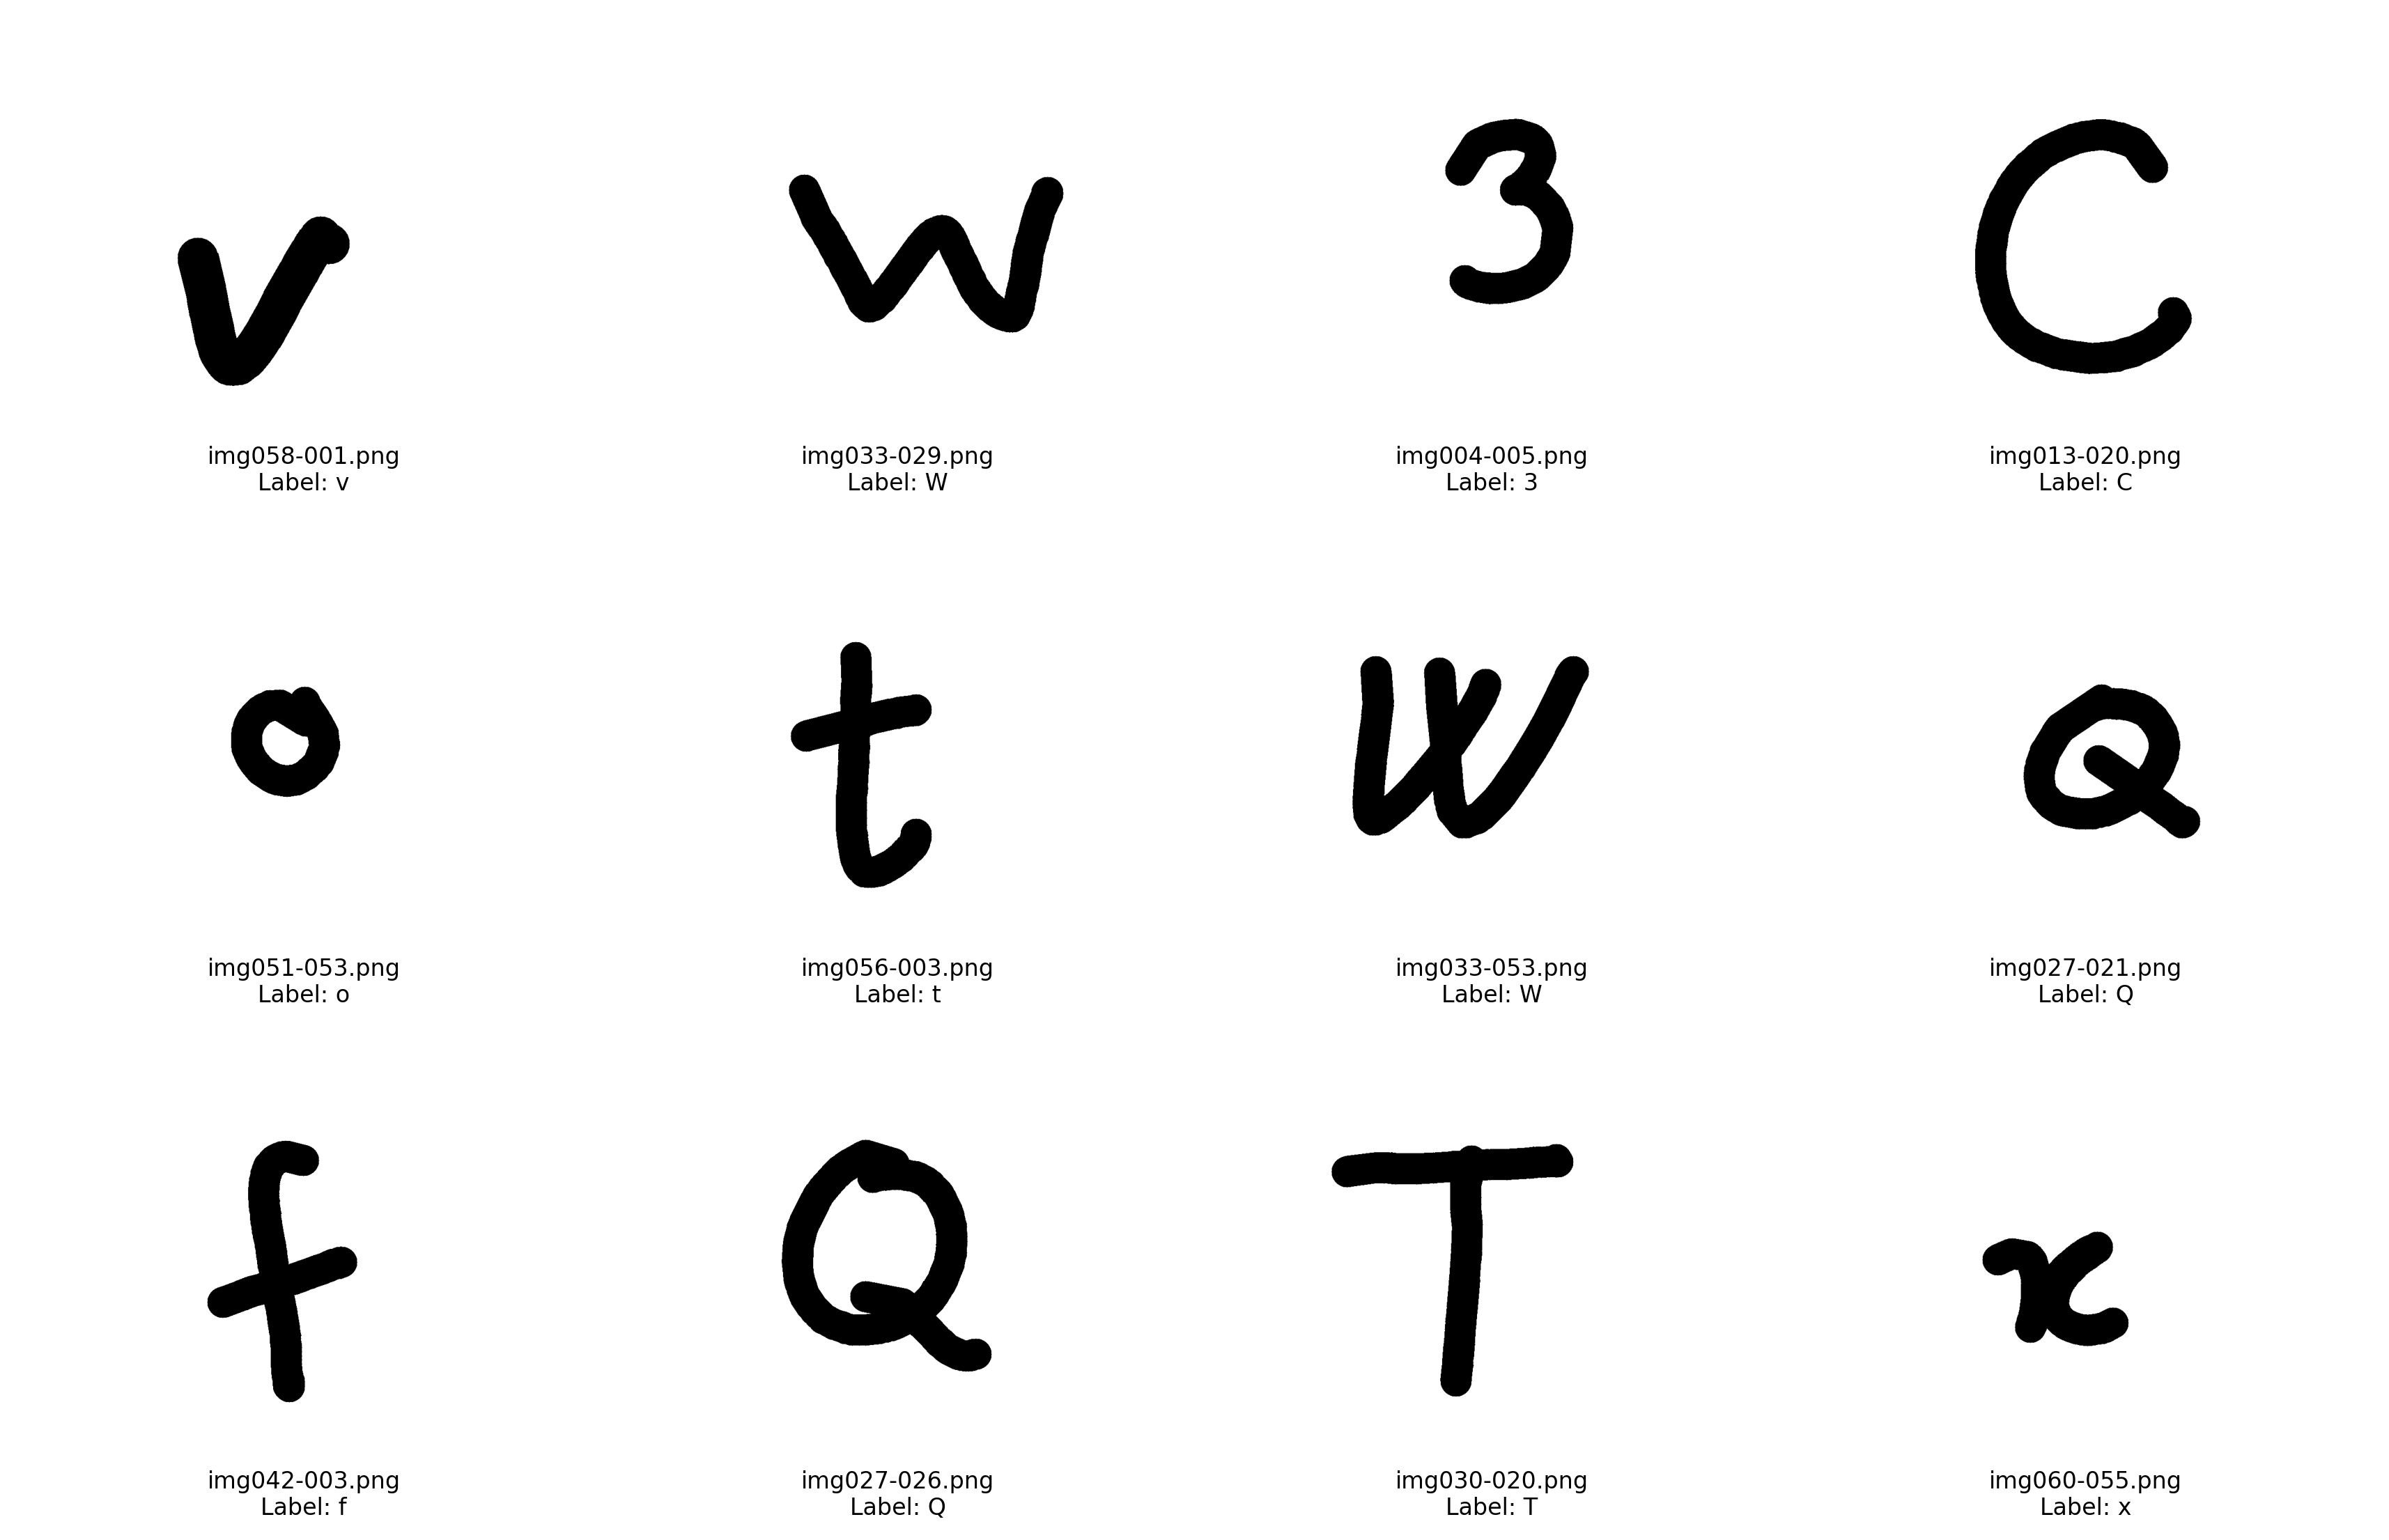
\includegraphics[width=0.99\columnwidth]{Figures/Results/HandwrittenCharacters/sample_handwritten_characters.png}
    \caption{Sample of handwritten digits from the Kaggle Handwritten Character Dataset}
\label{fig:sample_handwritten_characters}
\end{figure}

%%%%%%%%%%%%%%%%%%%%%%%%%%%%%
% PADDING STATISTICS TABLES %
%%%%%%%%%%%%%%%%%%%%%%%%%%%%%

\begin{table}[h]
\centering
\begin{tabular}{lcccccccccc}
Attribute & 0 & 1 & 2 & 3 & 4 & 5 & 6 & 7 & 8 & 9 \\
\hline
Left Padding (\%) & 19.88 & 35.18 & 19.57 & 18.88 & 22.26 & 21.97 & 26.65 & 20.19 & 25.12 & 24.80 \\
Right Padding (\%) & 15.81 & 31.44 & 15.17 & 22.27 & 19.23 & 13.83 & 18.96 & 22.54 & 18.29 & 24.12 \\
Top Padding (\%) & 15.97 & 15.46 & 14.09 & 16.49 & 17.85 & 18.65 & 8.97 & 24.35 & 17.32 & 22.29 \\
Bottom Padding (\%) & 14.16 & 13.14 & 17.04 & 12.54 & 11.17 & 13.44 & 19.81 & 4.70 & 11.62 & 6.36 \\
Left Padding (px) & 5.57 & 9.85 & 5.48 & 5.29 & 6.23 & 6.15 & 7.46 & 5.65 & 7.03 & 6.94 \\
Right Padding (px) & 4.43 & 8.80 & 4.25 & 6.24 & 5.38 & 3.87 & 5.31 & 6.31 & 5.12 & 6.75 \\
Top Padding (px) & 4.47 & 4.33 & 3.95 & 4.62 & 5.00 & 5.22 & 2.51 & 6.82 & 4.85 & 6.24 \\
Bottom Padding (px) & 3.97 & 3.68 & 4.77 & 3.51 & 3.13 & 3.76 & 5.55 & 1.32 & 3.25 & 1.78 \\
\end{tabular}
\caption{Training Set Padding Averages}
\label{app:MNIST_Training_Dataset_pixel_padding_stats}
\end{table}

\begin{table}[h]
\centering
\begin{tabular}{lcccccccccc}
Attribute & 0 & 1 & 2 & 3 & 4 & 5 & 6 & 7 & 8 & 9 \\
\hline
Left Padding (\%) & 20.25 & 35.91 & 19.78 & 19.48 & 22.23 & 21.95 & 26.00 & 20.49 & 25.53 & 24.78 \\
Right Padding (\%) & 15.91 & 31.92 & 15.52 & 22.69 & 19.69 & 13.87 & 17.97 & 23.06 & 18.80 & 24.10 \\
Top Padding (\%) & 15.94 & 15.49 & 13.93 & 16.42 & 17.96 & 18.61 & 8.92 & 24.00 & 17.27 & 22.21 \\
Bottom Padding (\%) & 14.39 & 13.09 & 16.72 & 12.63 & 11.00 & 13.21 & 19.86 & 4.90 & 11.62 & 6.40 \\
Left Padding (px) & 5.67 & 10.06 & 5.54 & 5.45 & 6.22 & 6.14 & 7.28 & 5.74 & 7.15 & 6.94 \\
Right Padding (px) & 4.46 & 8.94 & 4.34 & 6.35 & 5.51 & 3.88 & 5.03 & 6.46 & 5.26 & 6.75 \\
Top Padding (px) & 4.46 & 4.34 & 3.90 & 4.60 & 5.03 & 5.21 & 2.50 & 6.72 & 4.83 & 6.22 \\
Bottom Padding (px) & 4.03 & 3.66 & 4.68 & 3.54 & 3.08 & 3.70 & 5.56 & 1.37 & 3.25 & 1.79 \\
\end{tabular}
\caption{Testing Set Padding Averages}
\label{app:MNIST_Testing_Dataset_pixel_padding_stats}
\end{table}

We are interested in using our CNN trained on MNIST to predict the characters, then examine distances to predicted class centroids and compute statistics to establish if said distances help express uncertainty about characters that the network has not seen and does not know about e.g. letters of the alphabet.

Tables \ref{app:MNIST_Training_Dataset_pixel_padding_stats} and \ref{app:MNIST_Testing_Dataset_pixel_padding_stats} show padding as a percentage and average pixel value for training and testing datasets. It can be observed that in general digit 1 has larger left and right padding values compared to other digits. 
% discussion()
% MNIST_padding_stats.py
% commit 98f7eee
% repo git@github.com:dsikar/work-in-progress.git

Aggregate statistics for left, right, top, and bottom padding as percentages, including means and ranges, for the MNIST training and testing datasets:
\begin{itemize}
    \item \textbf{Training Set:}
    \begin{itemize}
        \item Left Padding: Mean = 23.45\%, Range = 18.88\% (digit 3) to 35.18\% (digit 1)
        \item Right Padding: Mean = 20.17\%, Range = 13.83\% (digit 5) to 31.44\% (digit 1)
        \item Top Padding: Mean = 17.14\%, Range = 8.97\% (digit 6) to 24.35\% (digit 7)
        \item Bottom Padding: Mean = 12.40\%, Range = 4.70\% (digit 7) to 19.81\% (digit 6)
    \end{itemize}
    \item \textbf{Testing Set:}
    \begin{itemize}
        \item Left Padding: Mean = 22.64\%, Range = 19.48\% (digit 3) to 35.91\% (digit 1)
        \item Right Padding: Mean = 20.35\%, Range = 13.87\% (digit 5) to 31.92\% (digit 1)
        \item Top Padding: Mean = 17.07\%, Range = 8.92\% (digit 6) to 24.00\% (digit 7)
        \item Bottom Padding: Mean = 12.38\%, Range = 4.90\% (digit 7) to 19.86\% (digit 6)
    \end{itemize}
\end{itemize}

% \begin{table}[h]
% \centering
% \begin{tabular}{lcccccccccc}
% Attribute & 0 & 1 & 2 & 3 & 4 & 5 & 6 & 7 & 8 & 9 \\
% \hline
% Left Padding (\%) & 20.25 & 35.91 & 19.78 & 19.48 & 22.23 & 21.95 & 26.00 & 20.49 & 25.53 & 24.78 \\
% Right Padding (\%) & 15.91 & 31.92 & 15.52 & 22.69 & 19.69 & 13.87 & 17.97 & 23.06 & 18.80 & 24.10 \\
% Top Padding (\%) & 15.94 & 15.49 & 13.93 & 16.42 & 17.96 & 18.61 & 8.92 & 24.00 & 17.27 & 22.21 \\
% Bottom Padding (\%) & 14.39 & 13.09 & 16.72 & 12.63 & 11.00 & 13.21 & 19.86 & 4.90 & 11.62 & 6.40 \\
% Left Padding (px) & 5.67 & 10.06 & 5.54 & 5.45 & 6.22 & 6.14 & 7.28 & 5.74 & 7.15 & 6.94 \\
% Right Padding (px) & 4.46 & 8.94 & 4.34 & 6.35 & 5.51 & 3.88 & 5.03 & 6.46 & 5.26 & 6.75 \\
% Top Padding (px) & 4.46 & 4.34 & 3.90 & 4.60 & 5.03 & 5.21 & 2.50 & 6.72 & 4.83 & 6.22 \\
% Bottom Padding (px) & 4.03 & 3.66 & 4.68 & 3.54 & 3.08 & 3.70 & 5.56 & 1.37 & 3.25 & 1.79 \\
% \end{tabular}
% \caption{Testing Set Padding Averages}
% \label{app:MNIST_Testing_Dataset_pixel_padding_stats}
% \end{table}

% MNIST_padding_stats
% git@github.com:dsikar/work-in-progress.git

% Should be the same as previous tables
% \begin{table}[h]
% \centering
% \begin{tabular}{lcccccccccc}
% Attribute & 0 & 1 & 2 & 3 & 4 & 5 & 6 & 7 & 8 & 9 \\
% \hline
% Left Padding (\%) & 19.88 & 35.18 & 19.57 & 18.88 & 22.26 & 21.97 & 26.65 & 20.19 & 25.12 & 24.80 \\
% Right Padding (\%) & 15.81 & 31.44 & 15.17 & 22.27 & 19.23 & 13.83 & 18.96 & 22.54 & 18.29 & 24.12 \\
% Top Padding (\%) & 15.97 & 15.46 & 14.09 & 16.49 & 17.85 & 18.65 & 8.97 & 24.35 & 17.32 & 22.29 \\
% Bottom Padding (\%) & 14.16 & 13.14 & 17.04 & 12.54 & 11.17 & 13.44 & 19.81 & 4.70 & 11.62 & 6.36 \\
% Left Padding (px) & 5.57 & 9.85 & 5.48 & 5.29 & 6.23 & 6.15 & 7.46 & 5.65 & 7.03 & 6.94 \\
% Right Padding (px) & 4.43 & 8.80 & 4.25 & 6.24 & 5.38 & 3.87 & 5.31 & 6.31 & 5.12 & 6.75 \\
% Top Padding (px) & 4.47 & 4.33 & 3.95 & 4.62 & 5.00 & 5.22 & 2.51 & 6.82 & 4.85 & 6.24 \\
% Bottom Padding (px) & 3.97 & 3.68 & 4.77 & 3.51 & 3.13 & 3.76 & 5.55 & 1.32 & 3.25 & 1.78 \\
% \end{tabular}
% \caption{Training Set Padding Averages}
% \end{table}




% Perturbed testing dataset
% \begin{table}[h]
% \centering
% \begin{tabular}{lcccccccccc}
% Attribute & 0 & 1 & 2 & 3 & 4 & 5 & 6 & 7 & 8 & 9 \\
% \hline
% Left Padding (\%) & 5.82 & 10.89 & 5.55 & 5.41 & 6.33 & 6.27 & 7.77 & 5.71 & 7.67 & 7.25 \\
% Right Padding (\%) & 3.54 & 8.76 & 3.43 & 5.86 & 4.75 & 2.89 & 4.20 & 5.88 & 4.60 & 6.30 \\
% Top Padding (\%) & 3.47 & 3.05 & 2.62 & 3.51 & 3.97 & 4.27 & 0.99 & 6.18 & 3.85 & 5.54 \\
% Bottom Padding (\%) & 2.46 & 1.78 & 3.17 & 1.79 & 1.25 & 1.99 & 4.17 & 0.30 & 1.47 & 0.44 \\
% Left Padding (px) & 1.63 & 3.05 & 1.55 & 1.52 & 1.77 & 1.76 & 2.18 & 1.60 & 2.15 & 2.03 \\
% Right Padding (px) & 0.99 & 2.45 & 0.96 & 1.64 & 1.33 & 0.81 & 1.18 & 1.65 & 1.29 & 1.76 \\
% Top Padding (px) & 0.97 & 0.85 & 0.73 & 0.98 & 1.11 & 1.20 & 0.28 & 1.73 & 1.08 & 1.55 \\
% Bottom Padding (px) & 0.69 & 0.50 & 0.89 & 0.50 & 0.35 & 0.56 & 1.17 & 0.08 & 0.41 & 0.12 \\
% \end{tabular}
% \caption{Testing Set Padding Averages}
% \label{app:MNIST_Testing_Dataset_pixel_padding_stats}
% \end{table}


%\subsection{Single digit stats}

% single_image_stats(img_np)
% Repo git@github.com:dsikar/work-in-progress.git
% Script MNIST_padding_stats.py

%%%%%%%%%%%%%%%%%%%%%%
% SINGLE DIGIT STATS %
%%%%%%%%%%%%%%%%%%%%%%

Figure \ref{fig:MNIST_training_index_0_label_5} shows the first digit in the MNIST training dataset. The padding statistics for left, right, top and bottom are 4, 4, 5, 3 pixels respectively, and 14.29\%, 14.29\%, 17.86\%, 10.71\% as proportions of the 28x28 size.

% [(14.285714285714285, 14.285714285714285, 17.857142857142858, 10.714285714285714, 4, 4, 5, 3)]})

%%%%%%%%%%%
% DIGIT 5 %
%%%%%%%%%%%
\begin{figure}[ht]
    \centering
    
\includegraphics[width=0.50\columnwidth]{Figures/Results/HandwrittenCharacters/MNIST_training_index_0_label_5.png}
    \caption{MNIST Training example index 0 (first example), label 5}
\label{fig:MNIST_training_index_0_label_5}
\end{figure}

Figure \ref{fig:Training_Digits_1_5} shows a random selection of training data that reflects the general trends shows in tables \ref{app:MNIST_Training_Dataset_pixel_padding_stats} and \ref{app:MNIST_Testing_Dataset_pixel_padding_stats}, e.g. digit 1 typically has wider left and right paddings compared to digit 5.

%%%%%%%%%%%%%%%%%%%%%%
% DIGIT 1 AND 5 ROWS %
%%%%%%%%%%%%%%%%%%%%%%

% MNIST_training_testing_ones.py

\begin{figure}[ht]
    \centering
    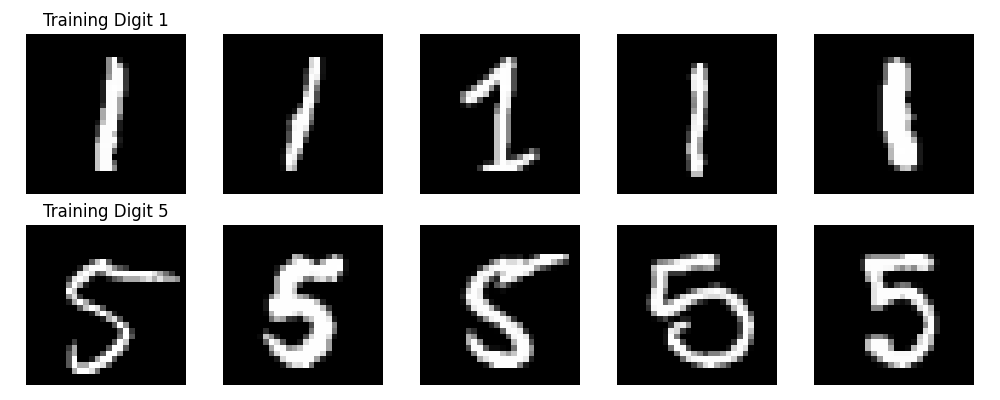
\includegraphics[width=0.99\columnwidth]{Figures/Results/HandwrittenCharacters/Training_Digits_1_5.png}
    \caption{Random selection of MNIST training data digits 1 on top row and 5 on bottom row}
\label{fig:Training_Digits_1_5}
\end{figure}

The left and top padding percentages in the MNIST training and testing datasets, as depicted in Figure \ref{fig:MNIST_training_testing_padding_plots}, reveal distinct trends across digits 0–9 that reflect the structural characteristics of handwritten digits. For left padding, both sets show a pronounced peak for digit 1 (training: 35.18\%, testing: 35.91\%), driven by its narrow, vertical shape, which leaves substantial horizontal space. This trend is consistent across sets, though testing values are slightly higher (e.g., 35.91\% vs. 35.18\%), suggesting minor positional variations. Other digits, such as 3 and 5, exhibit lower left padding (around 18–22\%), indicating wider or more centered shapes. Top padding, in contrast, shows greater variability, with digit 7 displaying the highest values (training: 24.35\%, testing: 24.00\%), reflecting its top-heavy strokes, while digit 6 has the lowest (training: 8.97\%, testing: 8.92\%), aligning with its bottom-heavy features. Across both padding types, training and testing sets are closely aligned, with mean differences under 1\% (left: 23.45\% vs. 22.64\%; top: 17.14\% vs. 17.07\%). 

%%%%%%%%%%%%%%%%%%%%%%%%%%%%%%%%%%%%
% MNIST LEFT AND TOP PADDING PLOTS %
%%%%%%%%%%%%%%%%%%%%%%%%%%%%%%%%%%%%

\begin{figure}[ht]
    \centering
    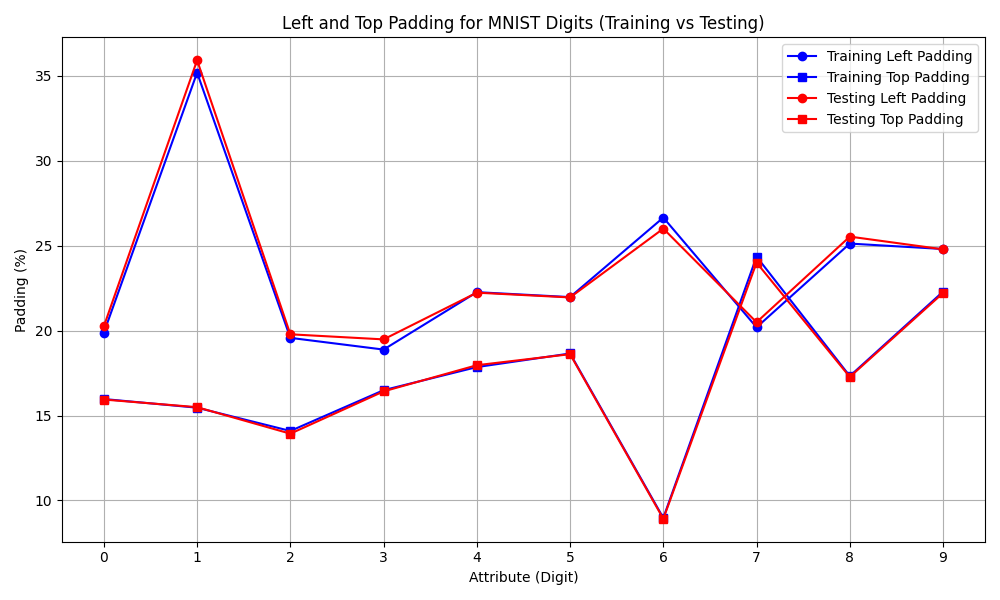
\includegraphics[width=0.99\columnwidth]{Figures/Results/HandwrittenCharacters/MNIST_training_testing_padding_plots.png}
    \caption{MNIST training and testing data left and top padding percentages i.e. padding in pixels / width|height (28 pixels)}
\label{fig:MNIST_training_testing_padding_plots}
\end{figure}

%\subsection{Converting the English Handwritten Characters to MNIST-like format}

%%%%%%%%%%%%%%%%%%%%%%%%%%%%%%%%%%%%%%%%%%%%%%%%%%%%%%%%%%%%%%%%%%%%%%
% CONVERTING the ENGLISH HANDWRITTEN CHARACTERS TO MNIST-LIKE FORMAT %
%%%%%%%%%%%%%%%%%%%%%%%%%%%%%%%%%%%%%%%%%%%%%%%%%%%%%%%%%%%%%%%%%%%%%%

The English Handwritten Characters dataset as previously mentioned are 1200 x 900 pixels in size, all RGB (3 channel) in PNG format, and need to be converted to 28x28 single channel grayscale images.

% Image Img/img004-005.png - Label: 3, Size: (1200, 900), Min/Max Pixel (grayscale): 0/255
% Image Img/img013-020.png - Label: C, Size: (1200, 900), Min/Max Pixel (grayscale): 0/255
% Image Img/img051-053.png - Label: o, Size: (1200, 900), Min/Max Pixel (grayscale): 0/255
% Image Img/img056-003.png - Label: t, Size: (1200, 900), Min/Max Pixel (grayscale): 0/255
% Image Img/img033-053.png - Label: W, Size: (1200, 900), Min/Max Pixel (grayscale): 0/255
% Image Img/img027-021.png - Label: Q, Size: (1200, 900), Min/Max Pixel (grayscale): 0/255
% Image Img/img042-003.png - Label: f, Size: (1200, 900), Min/Max Pixel (grayscale): 0/255
% Image Img/img027-026.png - Label: Q, Size: (1200, 900), Min/Max Pixel (grayscale): 0/255
% Image Img/img030-020.png - Label: T, Size: (1200, 900), Min/Max Pixel (grayscale): 0/255
% Image Img/img060-055.png - Label: x, Size: (1200, 900), Min/Max Pixel (grayscale): 0/255

% Padding for image (left%, right%, top%, bottom%, leftpx, rightpx, toppx, bottompx): (27.666666666666668, 41.833333333333336, 46.22222222222222, 13.777777777777779, 332, 502, 416, 124)
% Padding for image (left%, right%, top%, bottom%, leftpx, rightpx, toppx, bottompx): (30.666666666666664, 20.75, 36.333333333333336, 26.333333333333332, 368, 249, 327, 237)
% Padding for image (left%, right%, top%, bottom%, leftpx, rightpx, toppx, bottompx): (41.75, 35.5, 23.22222222222222, 33.0, 501, 426, 209, 297)
% Padding for image (left%, right%, top%, bottom%, leftpx, rightpx, toppx, bottompx): (30.416666666666664, 31.25, 23.333333333333332, 16.555555555555557, 365, 375, 210, 149)
% Padding for image (left%, right%, top%, bottom%, leftpx, rightpx, toppx, bottompx): (37.166666666666664, 43.5, 36.22222222222222, 37.666666666666664, 446, 522, 326, 339)
% Padding for image (left%, right%, top%, bottom%, leftpx, rightpx, toppx, bottompx): (31.0, 44.0, 25.666666666666664, 16.22222222222222, 372, 528, 231, 146)
% Padding for image (left%, right%, top%, bottom%, leftpx, rightpx, toppx, bottompx): (25.416666666666664, 32.75, 28.999999999999996, 27.88888888888889, 305, 393, 261, 251)
% Padding for image (left%, right%, top%, bottom%, leftpx, rightpx, toppx, bottompx): (38.916666666666664, 29.75, 35.66666666666667, 27.88888888888889, 467, 357, 321, 251)
% Padding for image (left%, right%, top%, bottom%, leftpx, rightpx, toppx, bottompx): (32.916666666666664, 40.5, 22.555555555555557, 15.666666666666668, 395, 486, 203, 141)
% Padding for image (left%, right%, top%, bottom%, leftpx, rightpx, toppx, bottompx): (29.416666666666668, 33.416666666666664, 22.333333333333332, 22.88888888888889, 353, 401, 201, 206)
% Padding for image (left%, right%, top%, bottom%, leftpx, rightpx, toppx, bottompx): (21.666666666666668, 35.5, 23.333333333333332, 17.0, 260, 426, 210, 153)
% Padding for image (left%, right%, top%, bottom%, leftpx, rightpx, toppx, bottompx): (31.666666666666664, 42.41666666666667, 44.0, 28.888888888888886, 380, 509, 396, 260)
% Average Left Padding %: 31.56, Range: 21.67–41.75

%%%%%%%%%%%%%%%%%
% PREPROCESSING %
%%%%%%%%%%%%%%%%%

Figure \ref{fig:english-handwritten-chracters-dataset-preprocessing} shows the preprocessing pipeline applied to the English handwritten characters dataset before neural network inference. The raw input character is 900×1200 pixels.

The pipeline standardizes an image for MNIST compatibility (28x28 pixels). It first verifies the input is a two-dimensional grayscale array. A threshold identifies foreground pixels, and the minimal bounding box is computed. The image is cropped to isolate the character. A scale factor is then calculated so that the longer side of the cropped region measures 22 pixels, preserving the original aspect ratio. The cropped image is resized using Lanczos resampling with this scale factor. Next, the pixel intensities are inverted, yielding a white character on a black background. Finally, the resized image is centered on a 28×28 canvas, producing the final MNIST-formatted image that aligns with the MNIST format used during the network's training phase


% he image is then cropped to remove excess whitespace, focusing only on the character itself. This cropped image varies in size depending on the character's shape and writing style. Next, the image is resized to 22×22 pixels using Lanczos resampling to preserve visual features while reducing dimensionality. In the final step, the image is inverted (changing black to white and vice versa) and padded with a 3-pixel border on all sides to create a standardized 28×28 pixel image. This standardization ensures the images match the input dimensions expected by the CNN, which has been trained on the MNIST dataset. The final inverted format, with the character appearing as white on a black background, aligns with the MNIST format used during the network's training phase.

% convert2MNISTFormat.ipynb
% Sample MNISTified images
% commit 03351e7

% import matplotlib.pyplot as plt
% import numpy as np

% # Data from the tables for Left Padding (%) for digits 0–9
% attributes = range(10)  # Digits 0 to 9
% training_left_padding = [19.88, 35.18, 19.57, 18.88, 22.26, 21.97, 26.65, 20.19, 25.12, 24.80]
% testing_left_padding = [20.25, 35.91, 19.78, 19.48, 22.23, 21.95, 26.00, 20.49, 25.53, 24.78]

% # Create the plot
% plt.figure(figsize=(10, 6))
% plt.plot(attributes, training_left_padding, 'b-o', label='Training Left Padding')
% plt.plot(attributes, testing_left_padding, 'r-o', label='Testing Left Padding')

% # Set labels and title
% plt.xlabel('Attribute (Digit)')
% plt.ylabel('Padding (%)')
% plt.title('Left Padding for MNIST Digits (Training vs Testing)')

% # Add legend
% plt.legend()

% # Add grid
% plt.grid(True)

% # Set x-ticks to show all integers 0–9
% plt.xticks(range(10))

% # Adjust layout and display
% plt.tight_layout()
% plt.show()

\begin{figure}[ht]
    \centering
    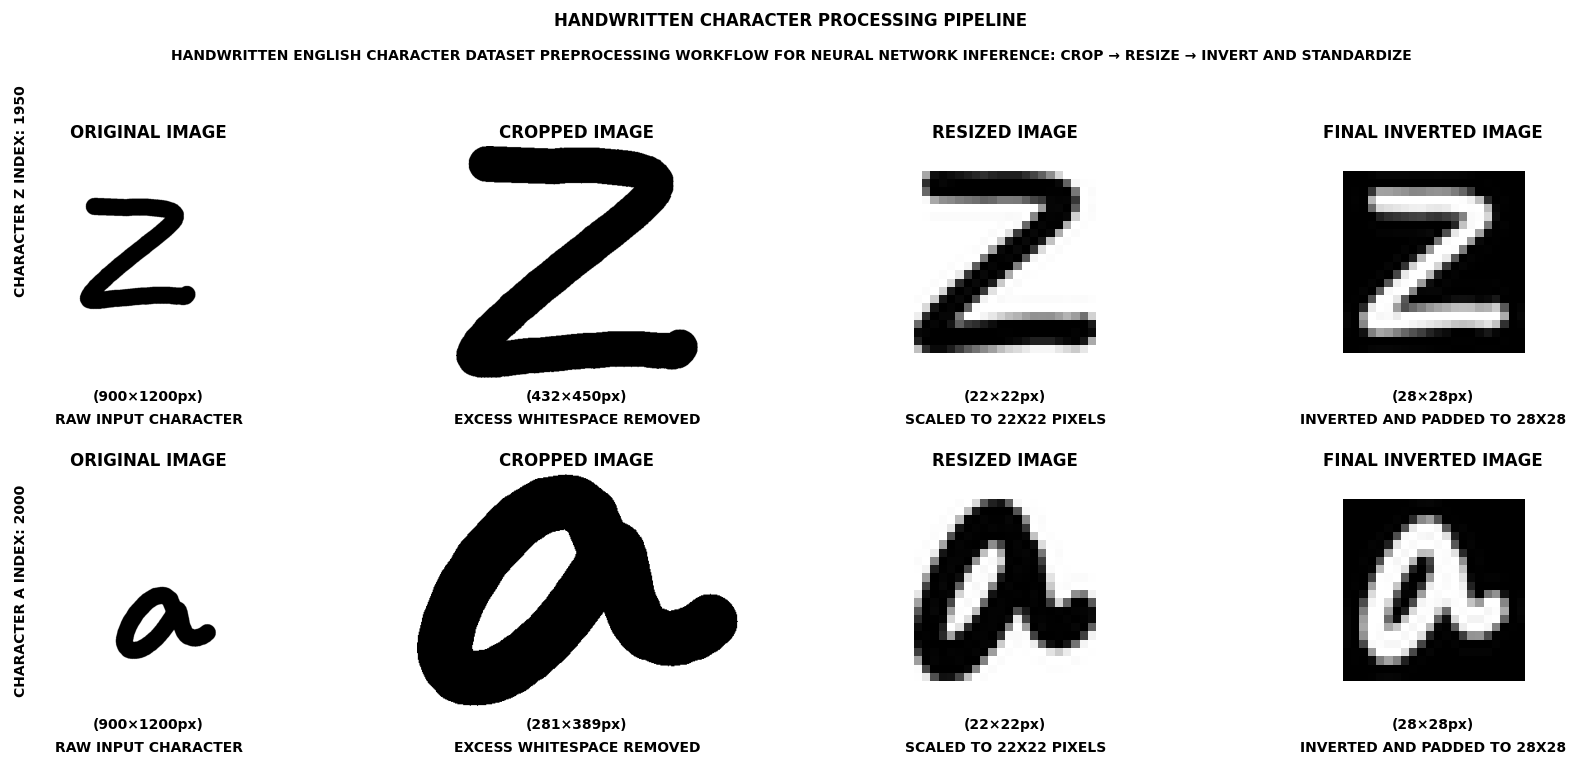
\includegraphics[width=0.99\columnwidth]{Figures/Results/HandwrittenCharacters/english-handwritten-chracters-dataset-preprocessing.png}
    \caption{Handwritten English Character Dataset "MNISTification" process, left to right, raw input character, character with excess white space removed, scaled (custom, based on character), and inverted (white font on black background), conforming to MNIST 28x28 pixel grayscale images.}
\label{fig:english-handwritten-chracters-dataset-preprocessing}
\end{figure}

Figures \ref{fig:mnistified-0-9}, \ref{fig:mnistified-A-Z} and \ref{fig:mnistified-a-z} shows samples of digits and upper and lower characters, processed to resemble the MNIST dataset.

% stopped here
% todos
% 1. processed digits 0 to 9, plot row OK
% 2. full alphabet lowercase, plot OK
% 3. full alphabe lowercase, plot OK
% 4. publish dataset
% 5. predict OK Accuracy 0.8727272727272727 (digits only)
% 6. softmax distances for digits correct / incorrect predictions
% 7. softmax distances for characters incorrect predictions nb correct N/A

%%%%%%%%%%%%%%%%%%%%%%%%%%%%%%%%%%%%%%%%%%%%%%%%%
% MNISTified English Handwritten Characters 0-9 %
%%%%%%%%%%%%%%%%%%%%%%%%%%%%%%%%%%%%%%%%%%%%%%%%%

% convert2MNISTFormat.ipynb - 0-9
% Sample MNISTified images
% commit 03351e7
\begin{figure}[ht]
    \centering
    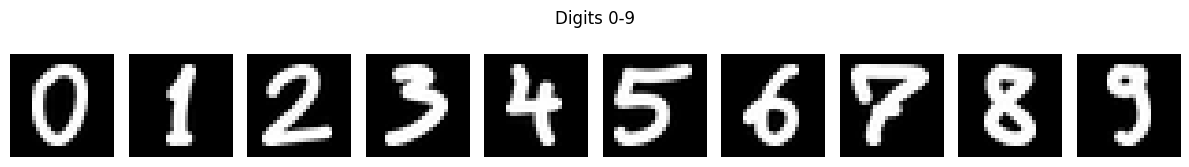
\includegraphics[width=0.99\columnwidth]{Figures/Results/HandwrittenCharacters/mnistified-0-9.png}
    \caption{MNISTified English Handwritten Characters 0-9}
\label{fig:mnistified-0-9}
\end{figure}


%%%%%%%%%%%%%%%%%%%%%%%%%%%%%%%%%%%%%%%%%%%%%%%%%
% MNISTified English Handwritten Characters A-Z %
%%%%%%%%%%%%%%%%%%%%%%%%%%%%%%%%%%%%%%%%%%%%%%%%%

% convert2MNISTFormat.ipynb - A-Z
% Sample MNISTified images
% commit 03351e7
\begin{figure}[ht]
    \centering
    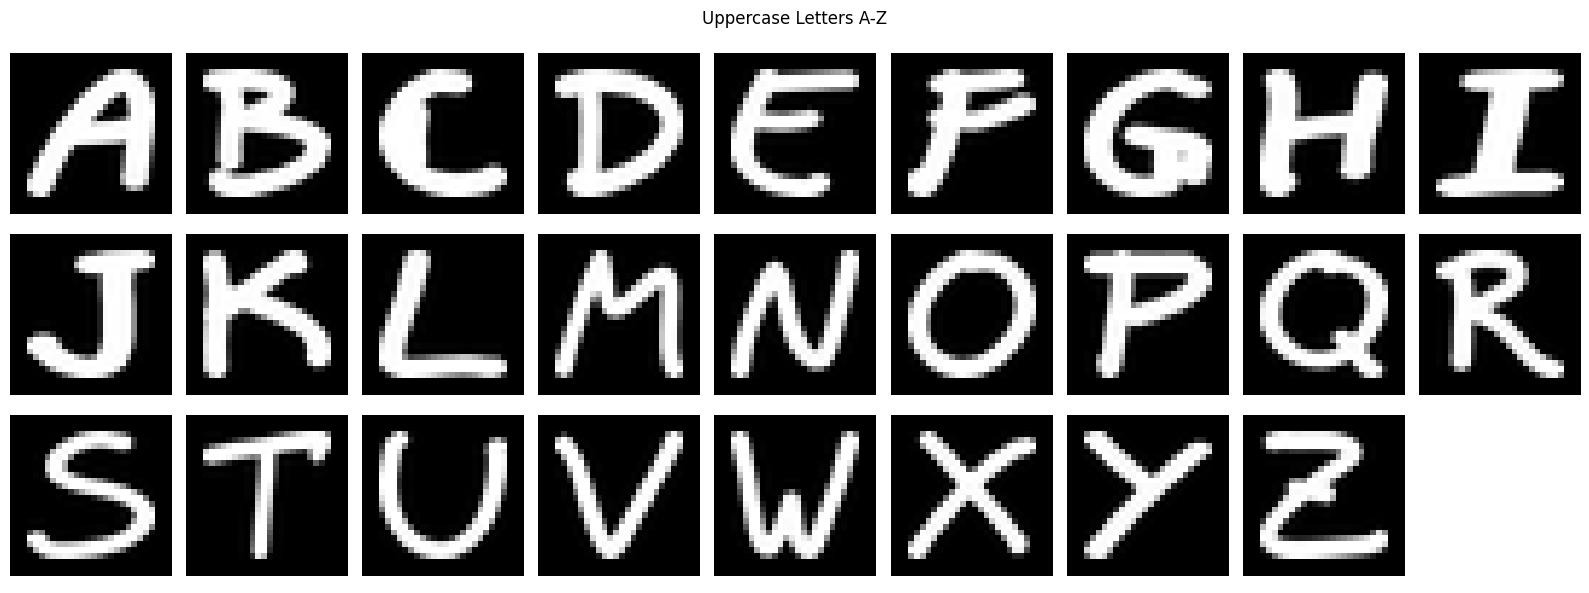
\includegraphics[width=0.99\columnwidth]{Figures/Results/HandwrittenCharacters/mnistified-A-Z.png}
    \caption{MNISTified English Handwritten Characters A-Z}
\label{fig:mnistified-A-Z}
\end{figure}


%%%%%%%%%%%%%%%%%%%%%%%%%%%%%%%%%%%%%%%%%%%%%%%%%
% MNISTified English Handwritten Characters a-z %
%%%%%%%%%%%%%%%%%%%%%%%%%%%%%%%%%%%%%%%%%%%%%%%%%

% convert2MNISTFormat.ipynb - a-z
% Sample MNISTified images
% commit 03351e7
\begin{figure}[ht]
    \centering
    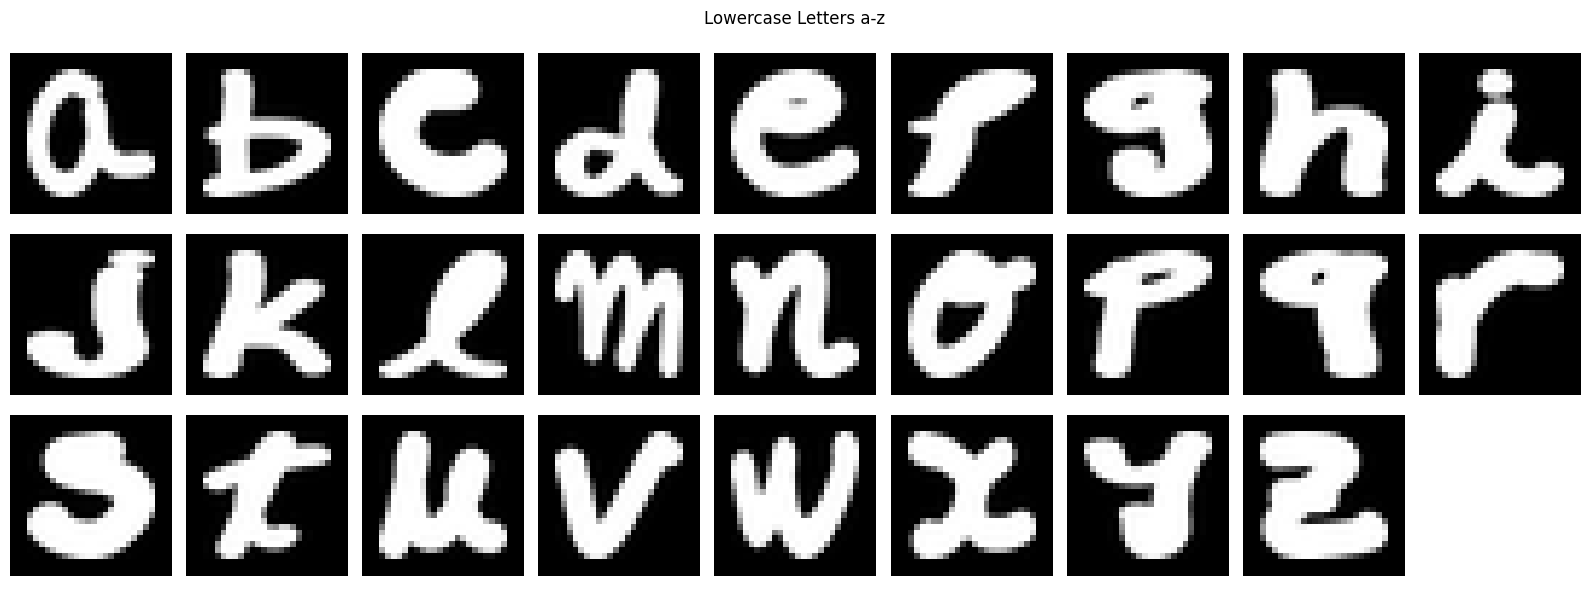
\includegraphics[width=0.99\columnwidth]{Figures/Results/HandwrittenCharacters/mnistified-a-z.png}
    \caption{MNISTified English Handwritten Characters a-z}
\label{fig:mnistified-a-z}
\end{figure}


%%%%%%%%%%%%%%%%%%%%%%%%%%%%%%%%%%%%%%%%%%
% HWC x MNIST LEFT AND TOP PADDING PLOTS %
%%%%%%%%%%%%%%%%%%%%%%%%%%%%%%%%%%%%%%%%%%

Figure \ref{fig:EHC_x_MNIST_training_testing_padding_plots} that digits 1, 9, and 8, in that order, exhibit the highest left-padding percentages, indicating they are narrower and thus need more horizontal space on the left to be centred. By contrast, 2, 1, and 5 are among the widest digits and therefore require less left padding. The top-padding values are relatively consistent across all digits, showing minimal variation in how they are positioned vertically. The MNISTified dataset is somewhat conformed to the MNIST dataset with respect to left padding, and also to right padding as can be observed in Figure \ref{fig:mnistified-0-9}.

% English_Handwritten_Charater_Digits_Padding_Stats.py
% plot_combined_padding(averages)
% commit 9906d82

\begin{figure}[ht]
    \centering
    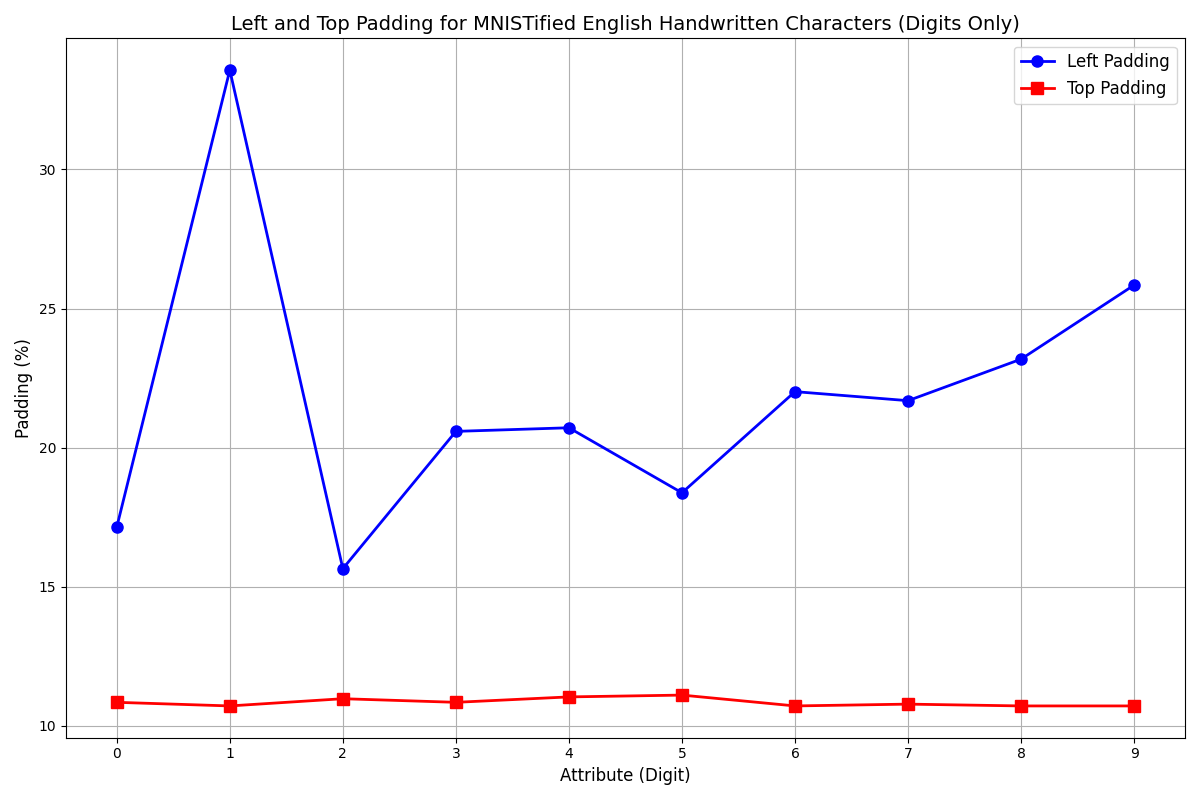
\includegraphics[width=0.99\columnwidth]{Figures/Results/HandwrittenCharacters/EHC_x_MNIST_training_testing_padding_plots.png}
    \caption{English Handwritten Characters (digits only) dataset conformed to MNIST layout}
\label{fig:EHC_x_MNIST_training_testing_padding_plots}
\end{figure}

%\subsection{MNISTified English Handwritten Character Results}

%%%%%%%%%%%%%%%%%%%%%%%%%%%%%%%%%%%%%%%%%%%%%%%%%%%%
% MNISTIFIED ENGLISH HANDWRITTEN CHARACTER RESULTS %
%%%%%%%%%%%%%%%%%%%%%%%%%%%%%%%%%%%%%%%%%%%%%%%%%%%%

Once conformed to the MNIST dataset, such that a trained CNN can be used for inference, the obtained accuracy on the English Handwritten Character digits is 87\%, compared to 98\% on the MNIST training dataset. 

Figure \ref{fig:english_handwritten_characters_digits_only_thresholds} shows the nearest distances (thresholds) for a class being misclassified e.g. the nearest misclassified digit 3 to digit 3 class centroid is 1.114 units away, and the nearest digit misclassified as a 6 is 0.251 units away from the 6 digit class centroid. Note there are no bars (blue or red) for digit 0 as no digit 0 was misclassified as another digit, and no other digits were misclassified as digit 0. Other similar cases are digits 2 and 5 (all digits correctly classified) and digit 4 (no digits misclassified as four), as can be seen in Figure \ref{fig:english_handwritten_characters_digits_only_confusion_matrix}, the confusion matrix for the MNISTified English Handwritten Character Dataset (Digits Only - 550 examples). 



The confusion matrix (Image 1) indicates high diagonal values, showing the model's accuracy for digit classification. Digits 0, 1, 2, 5, and 8 exhibit classification accuracy exceeding 95\%. The digit 7 displays significant misclassification patterns, with 10 instances classified as digit 3, 7 as digit 2, and 4 as digit 8. Digit 6 shows 14 cases misclassified as digit 5.
The threshold comparison (Image 2) presents distances of misclassified points on a logarithmic scale. The "Same Class" thresholds (blue) represent distances for points belonging to a class but misclassified elsewhere, while "Different Class" thresholds (red) show distances for points incorrectly assigned to a class. The largest disparity occurs for digits 4 and 5, where Different Class thresholds are minimal (0.007). Digits 6 and 9 demonstrate the highest Different Class thresholds (0.251 and 0.270), indicating more complex decision boundaries for these classes.

% ggit@github.com:dsikar/IJCNN-2025.git  mnist_alphabetic_character_analysis.py
% commit 91c8cc0
% Function call
% plot_thresholds_comparison(thresholds_same, thresholds_different, prefix="English Handwritten Characters Digits Only ", filename="english_handwritten_characters_digits_only_thresholds.png", save=True)
% # Saved as english_handwritten_characters_digits_only_thresholds.png
\begin{figure}[ht]
    \centering
    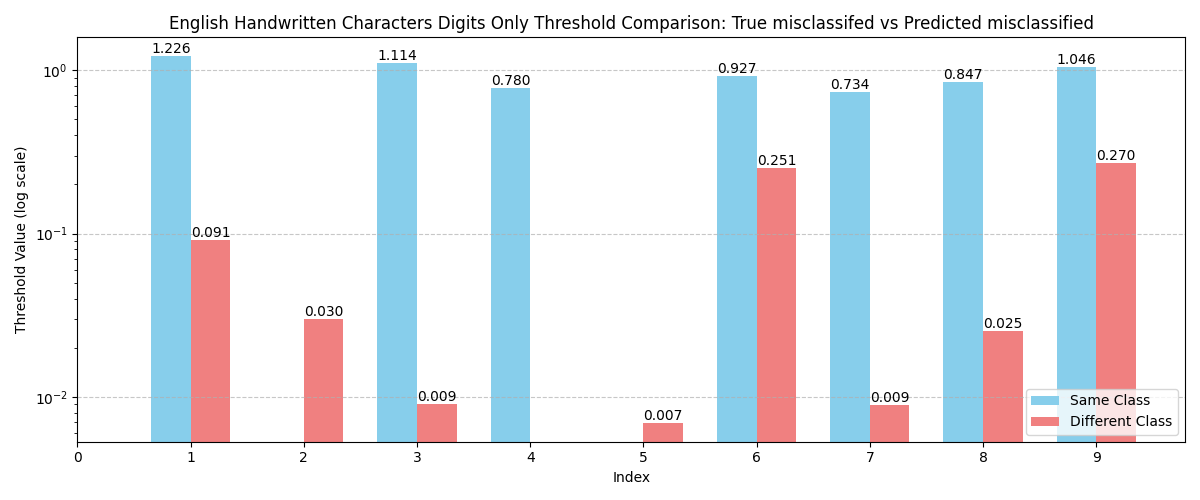
\includegraphics[width=0.99\columnwidth]{Figures/Results/HandwrittenCharacters/english_handwritten_characters_digits_only_thresholds.png}
    \caption{English Handwritten Characters (digits only) distances to class centroids, nearest "misprediction" of the true class (blue bars) and nearest misprediction of a predicted class}
\label{fig:english_handwritten_characters_digits_only_thresholds}
\end{figure}

% Function call
% # Confusion matrix for digits only
% confusion_matrix_digits = confusion_matrix(data_np, digits_only=True)
% plot_confusion_matrix(confusion_matrix_digits, prefix="English Handwritten Characters Digits Only ", filename="english_handwritten_characters_digits_only_confusion_matrix.png", save=True)
% # Saved as english_handwritten_characters_digits_only_confusion_matrix.png
\begin{figure}[ht]
    \centering
    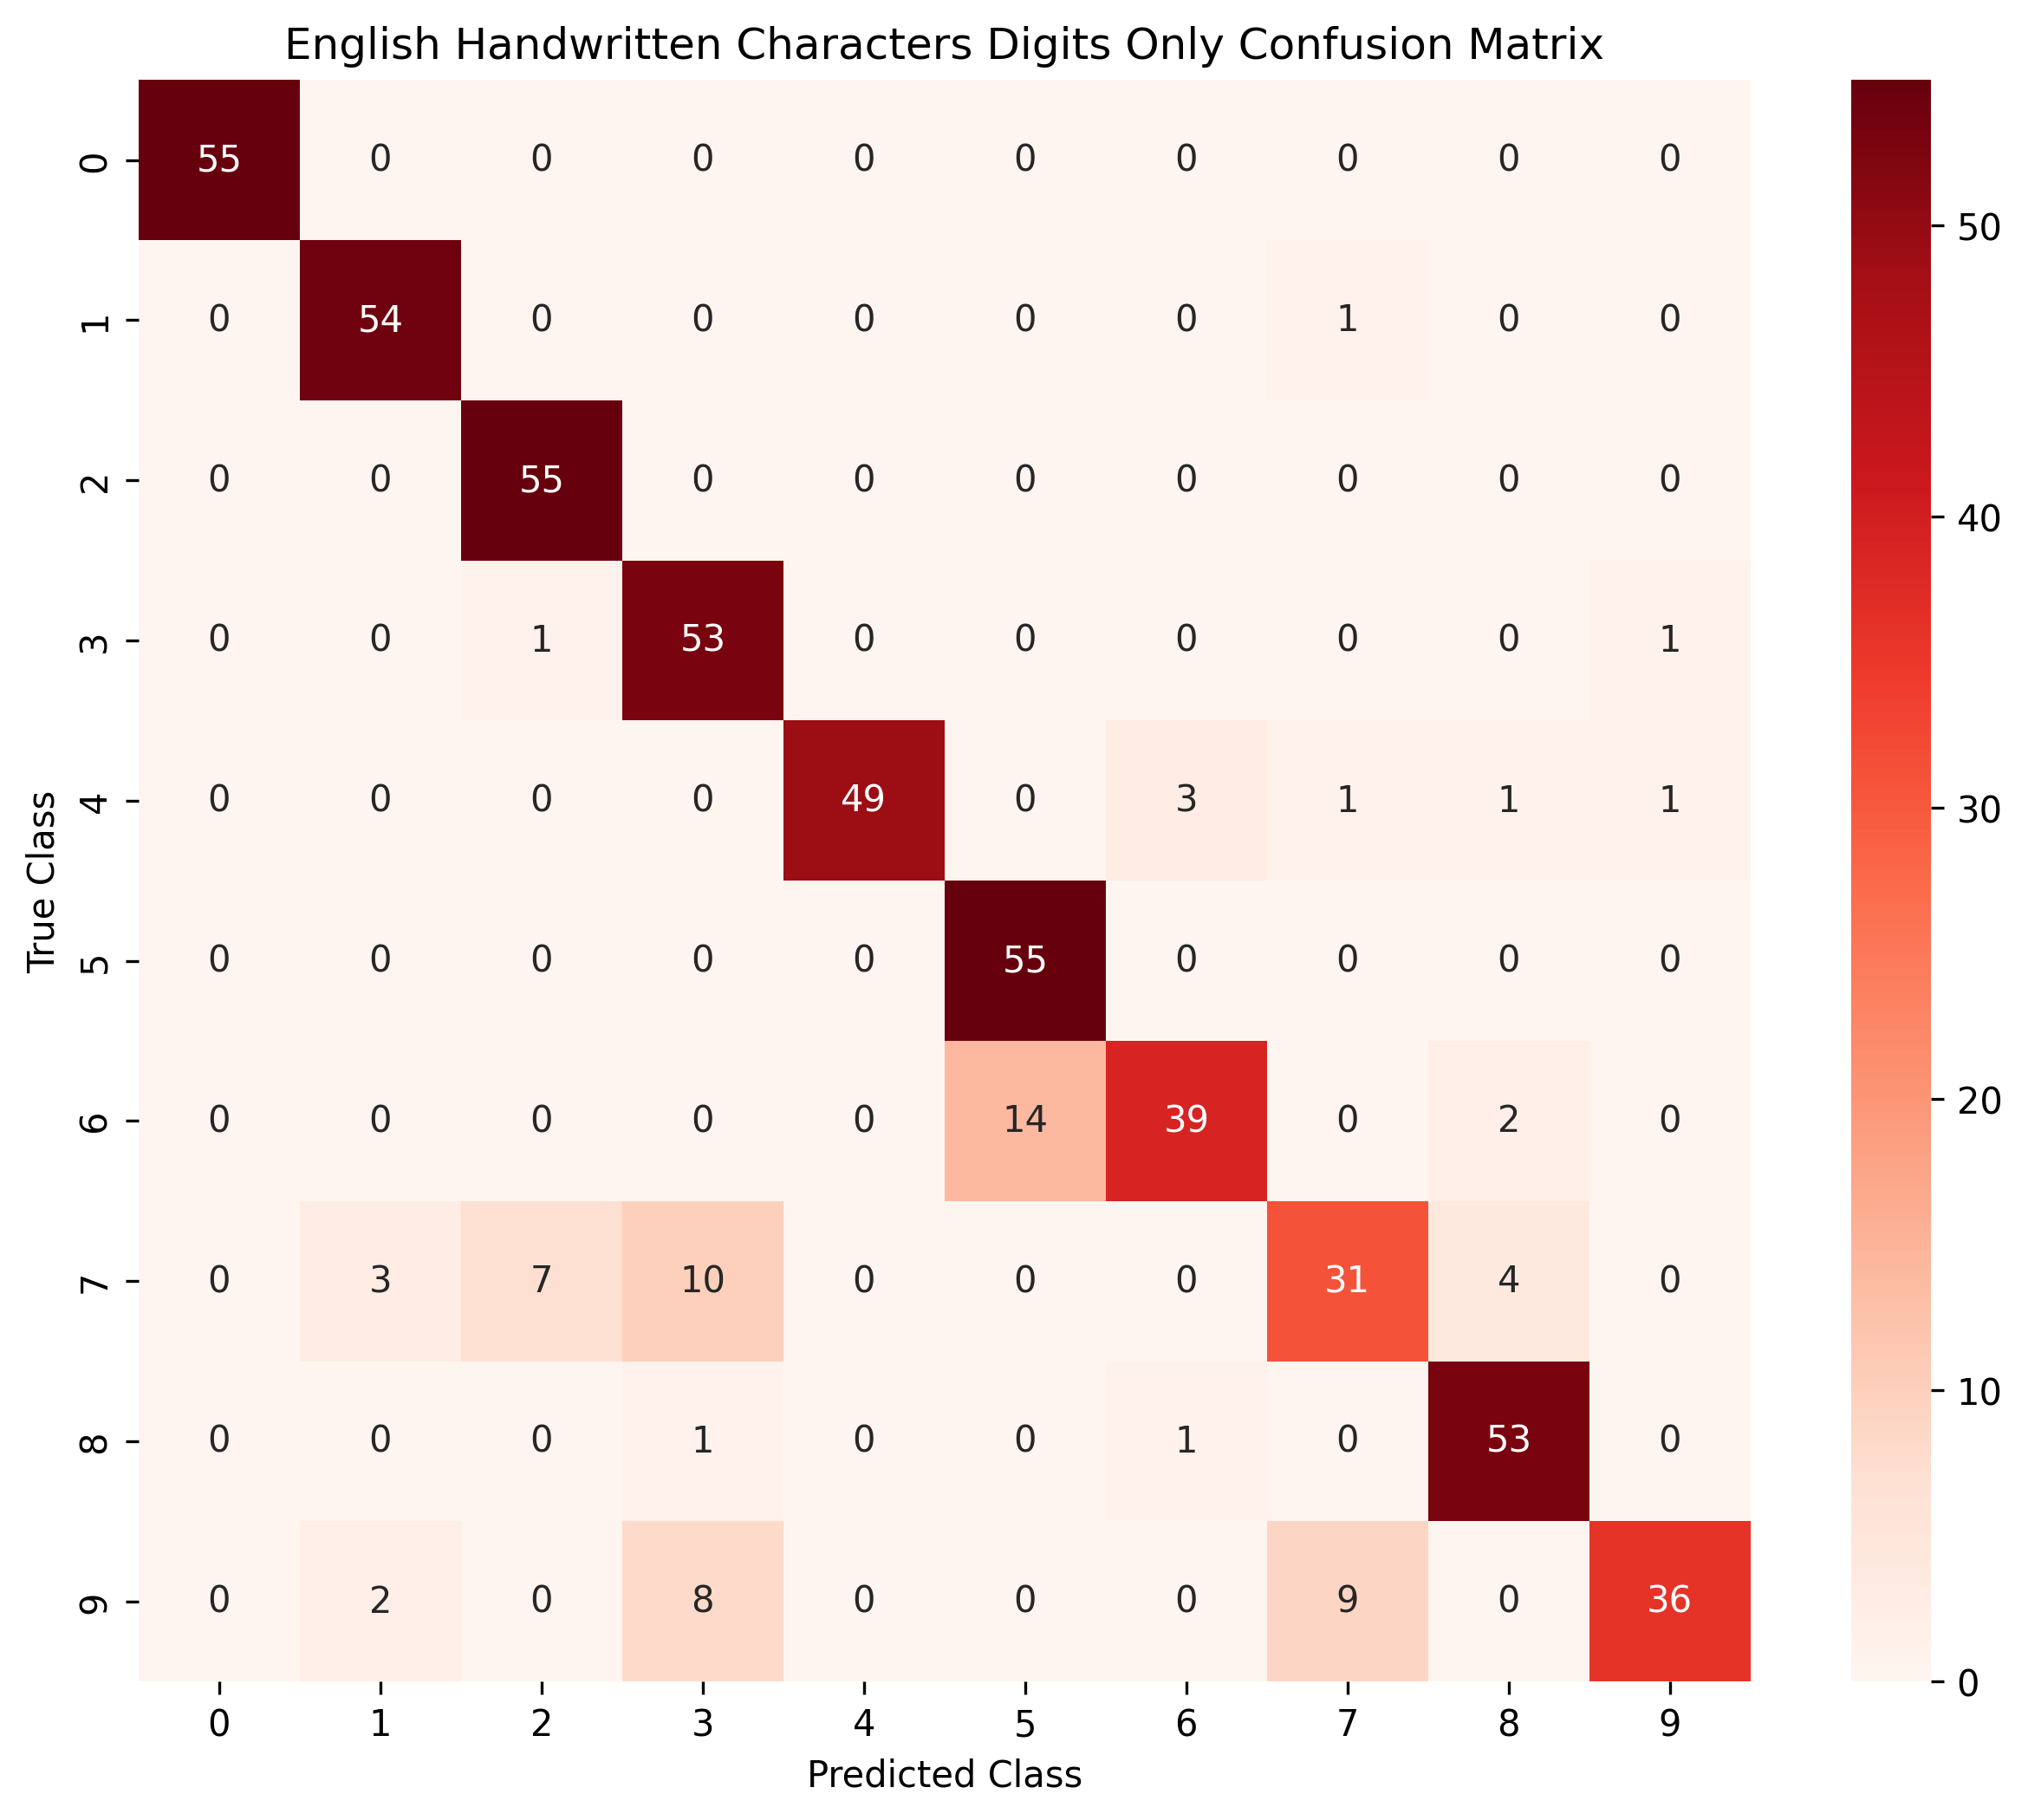
\includegraphics[width=0.99\columnwidth]{Figures/Results/HandwrittenCharacters/english_handwritten_characters_digits_only_confusion_matrix.png}
    \caption{English Handwritten Characters (digits only) confusion matrix for 550 predictions}
\label{fig:english_handwritten_characters_digits_only_confusion_matrix}
\end{figure}


% Digit 0: Number of alphabetic characters predicted as this digit: 528
% Digit 0: Minimum distance: 0.0016648656067618573
% Digit 0: Average distance: 0.16058877589020398
% Digit 0: Original index of the alphabetic character with min distance: 675
% Digit 0: Closest alphabetic character is 'C' (class 12)
% Digit 1: Number of alphabetic characters predicted as this digit: 365
% Digit 1: Minimum distance: 0.003745016885533488
% Digit 1: Average distance: 0.22722867838585623
% Digit 1: Original index of the alphabetic character with min distance: 3082
% Digit 1: Closest alphabetic character is 'u' (class 56)
% Digit 2: Number of alphabetic characters predicted as this digit: 242
% Digit 2: Minimum distance: 0.008925071596907863
% Digit 2: Average distance: 0.20964367917220236
% Digit 2: Original index of the alphabetic character with min distance: 3403
% Digit 2: Closest alphabetic character is 'z' (class 61)
% Digit 3: Number of alphabetic characters predicted as this digit: 85
% Digit 3: Minimum distance: 0.010936401745817276
% Digit 3: Average distance: 0.36543237233574044
% Digit 3: Original index of the alphabetic character with min distance: 1056
% Digit 3: Closest alphabetic character is 'J' (class 19)
% Digit 4: Number of alphabetic characters predicted as this digit: 493
% Digit 4: Minimum distance: 0.005890099717802539
% Digit 4: Average distance: 0.14786566703699247
% Digit 4: Original index of the alphabetic character with min distance: 568
% Digit 4: Closest alphabetic character is 'A' (class 10)


% ALphabetic characters distance to centroids
% alpha_thresholds, alpha_indexes, alpha_avg_distances = find_thresholds_alphabetic_only(data_np)

% plot_alphabetic_distances(alpha_thresholds, alpha_avg_distances, prefix="English Handwritten Alphabetic Characters ", filename="english_handwritten_characters_alphabetic_only_thresholds", save=True)
% # Saved as english_handwritten_characters_alphabetic_only_thresholds.png

\begin{figure}[ht]
    \centering
    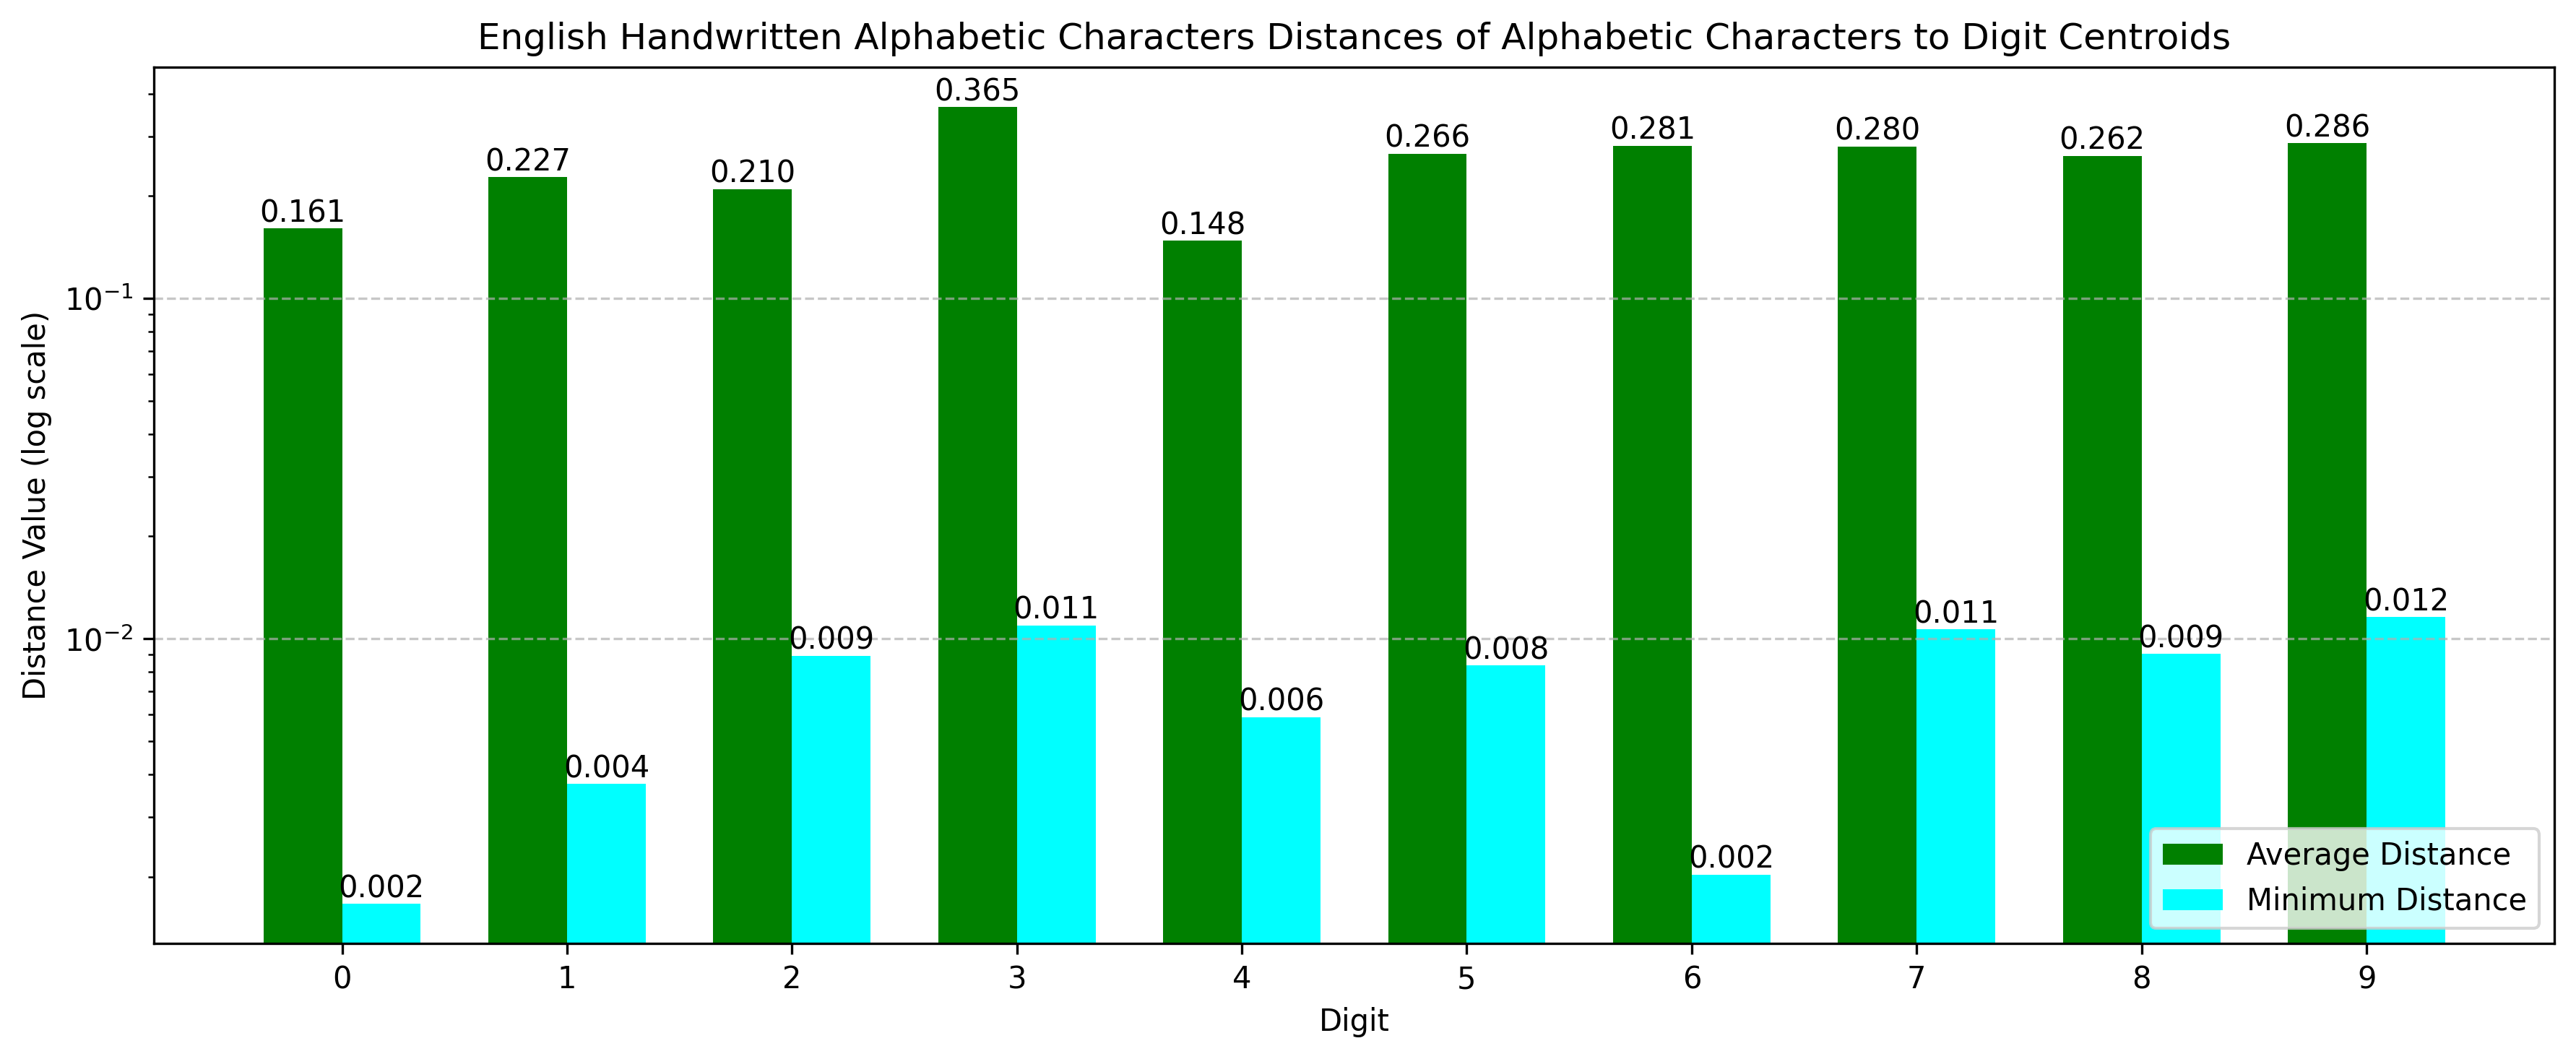
\includegraphics[width=0.99\columnwidth]{Figures/Results/HandwrittenCharacters/english_handwritten_characters_alphabetic_only_thresholds.png}
    \caption{English Handwritten Alphabetic Characters average and minimum distances to digit class centroids, where all examples have are "misclassified" given network was trained on digits only}
\label{fig:english_handwritten_characters_alphabetic_only_thresholds}
\end{figure}

% \begin{sidewaystable}[h]
% \centering
% \caption{Alphabetic Character Prediction Threshold Table}
% \begin{tabular}{c *{10}{S[table-format=3.0]@{\ (\si{\percent})}}
%                 S[table-format=4.0]@{\ (\si{\percent})} 
%                 S[table-format=4.0]@{\ (\si{\percent})}}
% \toprule
% {Thresh} & {0 (\%)} & {1 (\%)} & {2 (\%)} & {3 (\%)} & {4 (\%)} & {5 (\%)} & {6 (\%)} & {7 (\%)} & {8 (\%)} & {9 (\%)} & {TBT (\%)} & {TAT (\%)} \\
% \midrule
% 0.80 & 528 & 365 & 242 & 85 & 493 & 239 & 223 & 108 & 517 & 60 & 2860 & 0 \\ % Totals row, TAT = 0%
% 0.70 & 518 {(\SI{98.1}{\percent})} & 359 {(\SI{98.4}{\percent})} & 236 {(\SI{97.5}{\percent})} & 81 {(\SI{95.3}{\percent})} & 481 {(\SI{97.6}{\percent})} & 229 {(\SI{95.8}{\percent})} & 212 {(\SI{95.1}{\percent})} & 104 {(\SI{96.3}{\percent})} & 508 {(\SI{98.3}{\percent})} & 58 {(\SI{96.7}{\percent})} & 2786 {(\SI{97.4}{\percent})} & 74 {(\SI{2.6}{\percent})} \\
% 0.60 & 497 {(\SI{94.1}{\percent})} & 333 {(\SI{91.2}{\percent})} & 217 {(\SI{89.7}{\percent})} & 68 {(\SI{80.0}{\percent})} & 461 {(\SI{93.5}{\percent})} & 205 {(\SI{85.8}{\percent})} & 195 {(\SI{87.4}{\percent})} & 93 {(\SI{86.1}{\percent})} & 459 {(\SI{88.8}{\percent})} & 51 {(\SI{85.0}{\percent})} & 2579 {(\SI{90.2}{\percent})} & 281 {(\SI{9.8}{\percent})} \\
% 0.50 & 470 {(\SI{89.0}{\percent})} & 304 {(\SI{83.3}{\percent})} & 201 {(\SI{83.1}{\percent})} & 52 {(\SI{61.2}{\percent})} & 440 {(\SI{89.2}{\percent})} & 184 {(\SI{77.0}{\percent})} & 174 {(\SI{78.0}{\percent})} & 87 {(\SI{80.6}{\percent})} & 414 {(\SI{80.1}{\percent})} & 47 {(\SI{78.3}{\percent})} & 2373 {(\SI{83.0}{\percent})} & 487 {(\SI{17.0}{\percent})} \\
% 0.40 & 442 {(\SI{83.7}{\percent})} & 272 {(\SI{74.5}{\percent})} & 181 {(\SI{74.8}{\percent})} & 44 {(\SI{51.8}{\percent})} & 420 {(\SI{85.2}{\percent})} & 157 {(\SI{65.7}{\percent})} & 153 {(\SI{68.6}{\percent})} & 75 {(\SI{69.4}{\percent})} & 365 {(\SI{70.6}{\percent})} & 37 {(\SI{61.7}{\percent})} & 2146 {(\SI{75.0}{\percent})} & 714 {(\SI{25.0}{\percent})} \\
% 0.30 & 407 {(\SI{77.1}{\percent})} & 238 {(\SI{65.2}{\percent})} & 167 {(\SI{69.0}{\percent})} & 38 {(\SI{44.7}{\percent})} & 397 {(\SI{80.5}{\percent})} & 141 {(\SI{59.0}{\percent})} & 124 {(\SI{55.6}{\percent})} & 61 {(\SI{56.5}{\percent})} & 317 {(\SI{61.3}{\percent})} & 33 {(\SI{55.0}{\percent})} & 1923 {(\SI{67.2}{\percent})} & 937 {(\SI{32.8}{\percent})} \\
% 0.20 & 365 {(\SI{69.1}{\percent})} & 206 {(\SI{56.4}{\percent})} & 147 {(\SI{60.7}{\percent})} & 25 {(\SI{29.4}{\percent})} & 368 {(\SI{74.6}{\percent})} & 122 {(\SI{51.0}{\percent})} & 98 {(\SI{43.9}{\percent})} & 48 {(\SI{44.4}{\percent})} & 253 {(\SI{48.9}{\percent})} & 27 {(\SI{45.0}{\percent})} & 1659 {(\SI{58.0}{\percent})} & 1201 {(\SI{42.0}{\percent})} \\
% 0.10 & 320 {(\SI{60.6}{\percent})} & 154 {(\SI{42.2}{\percent})} & 127 {(\SI{52.5}{\percent})} & 16 {(\SI{18.8}{\percent})} & 314 {(\SI{63.7}{\percent})} & 100 {(\SI{41.8}{\percent})} & 76 {(\SI{34.1}{\percent})} & 32 {(\SI{29.6}{\percent})} & 183 {(\SI{35.4}{\percent})} & 22 {(\SI{36.7}{\percent})} & 1344 {(\SI{47.0}{\percent})} & 1516 {(\SI{53.0}{\percent})} \\
% 0.05 & 272 {(\SI{51.5}{\percent})} & 125 {(\SI{34.2}{\percent})} & 111 {(\SI{45.9}{\percent})} & 10 {(\SI{11.8}{\percent})} & 274 {(\SI{55.6}{\percent})} & 77 {(\SI{32.2}{\percent})} & 57 {(\SI{25.6}{\percent})} & 22 {(\SI{20.4}{\percent})} & 140 {(\SI{27.1}{\percent})} & 18 {(\SI{30.0}{\percent})} & 1106 {(\SI{38.7}{\percent})} & 1754 {(\SI{61.3}{\percent})} \\
% 0.02 & 228 {(\SI{43.2}{\percent})} & 101 {(\SI{27.7}{\percent})} & 71 {(\SI{29.3}{\percent})} & 8 {(\SI{9.4}{\percent})} & 240 {(\SI{48.7}{\percent})} & 56 {(\SI{23.4}{\percent})} & 30 {(\SI{13.5}{\percent})} & 18 {(\SI{16.7}{\percent})} & 12 {(\SI{2.3}{\percent})} & 10 {(\SI{16.7}{\percent})} & 774 {(\SI{27.1}{\percent})} & 2086 {(\SI{72.9}{\percent})} \\
% \bottomrule
% \end{tabular}
% \end{sidewaystable}

% data from
%np.save('data/grok_0.8_0.02_alphabetic_prediction_thresholds.npy', alpha_threshold_table)

\begin{table}[ht]
\centering
\caption{Alphabetic Character Prediction Threshold Table: Percentages (top) and Numeric Values (bottom)}
\label{tab:combined}
\scriptsize
\begin{tabular}{lccccccccccccc}
\toprule
\multicolumn{13}{c}{\textbf{Percentages (relative to baseline at 0.80)}} \\
\midrule
Thresh & 0 (\%) & 1 (\%) & 2 (\%) & 3 (\%) & 4 (\%) & 5 (\%) & 6 (\%) & 7 (\%) & 8 (\%) & 9 (\%) & TBT (\%) & TAT (\%) \\
\midrule
0.80   & 100.0  & 100.0  & 100.0  & 100.0  & 100.0  & 100.0  & 100.0  & 100.0  & 100.0  & 100.0  & 100.0   & 0.0   \\
0.70   & 98.1   & 98.2   & 97.5   & 95.3   & 97.5   & 95.8   & 95.2   & 96.3   & 98.1   & 96.7   & 97.4    & 2.6   \\
0.60   & 94.2   & 91.2   & 89.7   & 80.0   & 93.5   & 85.8   & 87.5   & 86.1   & 88.8   & 85.0   & 90.2    & 9.8   \\
0.50   & 89.0   & 83.3   & 83.1   & 61.2   & 89.2   & 77.0   & 78.0   & 80.6   & 80.0   & 78.3   & 82.9    & 17.1  \\
0.40   & 83.7   & 74.5   & 74.8   & 51.8   & 85.3   & 65.6   & 68.6   & 69.4   & 70.6   & 61.7   & 75.0    & 25.0  \\
0.30   & 77.1   & 65.2   & 69.0   & 44.7   & 80.6   & 58.9   & 55.6   & 56.5   & 61.3   & 55.0   & 67.2    & 32.8  \\
0.20   & 69.2   & 56.4   & 60.7   & 29.4   & 74.7   & 51.1   & 44.0   & 44.4   & 48.9   & 45.0   & 58.0    & 42.0  \\
0.10   & 60.6   & 42.2   & 52.5   & 18.8   & 63.8   & 41.8   & 34.1   & 29.6   & 35.4   & 36.7   & 47.1    & 52.9  \\
0.05   & 51.5   & 34.3   & 45.9   & 11.8   & 55.6   & 32.2   & 25.6   & 20.4   & 27.1   & 30.0   & 38.7    & 61.3  \\
0.02   & 43.2   & 27.7   & 29.4   & 9.4    & 48.7   & 23.4   & 13.5   & 16.7   & 2.3    & 16.7   & 27.1    & 72.9  \\
\midrule
\multicolumn{13}{c}{\textbf{Numeric Values}} \\
\midrule
Thresh & 0 & 1 & 2 & 3 & 4 & 5 & 6 & 7 & 8 & 9 & TBT & TAT \\
\midrule
0.80   & 528 & 365 & 242 & 85  & 493 & 239 & 223 & 108 & 517 & 60  & 2860 & 0   \\
0.70   & 518 & 359 & 236 & 81  & 481 & 229 & 212 & 104 & 508 & 58  & 2786 & 74  \\
0.60   & 497 & 333 & 217 & 68  & 461 & 205 & 195 & 93  & 459 & 51  & 2579 & 281 \\
0.50   & 470 & 304 & 201 & 52  & 440 & 184 & 174 & 87  & 414 & 47  & 2373 & 487 \\
0.40   & 442 & 272 & 181 & 44  & 420 & 157 & 153 & 75  & 365 & 37  & 2146 & 714 \\
0.30   & 407 & 238 & 167 & 38  & 397 & 141 & 124 & 61  & 317 & 33  & 1923 & 937 \\
0.20   & 365 & 206 & 147 & 25  & 368 & 122 & 98  & 48  & 253 & 27  & 1659 & 1201\\
0.10   & 320 & 154 & 127 & 16  & 314 & 100 & 76  & 32  & 183 & 22  & 1344 & 1516\\
0.05   & 272 & 125 & 111 & 10  & 274 & 77  & 57  & 22  & 140 & 18  & 1106 & 1754\\
0.02   & 228 & 101 & 71  & 8   & 240 & 56  & 30  & 18  & 12  & 10  & 774  & 2086\\
\bottomrule
\end{tabular}
\label{app:alphabetic_mnist_cnn_misclassifications}
\end{table}

Table \ref{app:alphabetic_mnist_cnn_misclassifications} displays data from the MNIST CNN classifier applied to alphabetic characters from the English Handwritten Character dataset. Note all classifications are incorrect because there is no true class for alphabetic characters. The upper table shows percentages calculated relative to the total examples baseline row at threshold 0.80. In the baseline, each digit column and TBT (Total below threshold) are 100.0\%, i.e. all examples are below threshold and TAT (total above threshold is 0.0\% i.e. no examples are above threshold, meaning no examples are classed as "don't know". In the following rows, the percentages for digit columns and TBT decrease as the threshold value decreases, while the percentage for TAT increases correspondingly, as more examples are set to "don't know". The aim is to set the threshold at a level that would exclude the maximum number of alphabetic characters, while still making the model usable.

The lower table presents the corresponding raw counts. At threshold 0.80, the digit counts sum to 2860 with TAT equal to 0. As the threshold value is reduced, the counts in each digit column decrease. Simultaneously, the value for TBT declines and the count for TAT increases. The change in values is consistent across all digit columns. The two tables together provide both normalized and absolute perspectives on the distribution of predictions as a function of the distance threshold.

The baseline row contains counts of 528, 365, 242, 85, 493, 239, 223, 108, 517, and 60 for digits 0 through 9, respectively. Counts in columns 0, 4, and 8 record 528, 493, and 517, while counts in columns 3, 7, and 9 record 85, 108, and 60. These values indicate that misclassifications resulting in digits 0, 4, and 8 occur in a greater number of instances than those resulting in digits 3, 7, and 9.

The impact of having unknown data can be assessed by referencing table \ref{app:enhanced_threshold_analysis}, where at a threshold of 0.05 the accuracy on the remaining data (91\%) is close to 100\%), corresponding to approximately 55k examples. The number of alphabetic characters where the softmax output is still below threshold is about 1k, so given the proportions, it would impact the accuracy in the single digit order of magnitude, and also decrease the ratio of correct / incorrect predictions up to threshold.

\begin{table*}[ht]
\centering
\tiny
\caption{Enhanced Threshold Analysis with Meta Metrics. 
Please zoom in for details. Key columns:
\textbf{Thresh}: Class threshold;
\textbf{Ret\%}: Retention percentage;
\textbf{Acc\%}: Accuracy percentage;
\textbf{Corr}: Correct predictions retained;
\textbf{Incor}: Incorrect predictions retained;
\textbf{CLost}: Cumulative correct lost;
\textbf{CElim}: Cumulative incorrect eliminated;
\textbf{Ratio}: Correct:Incorrect ratio;
\textbf{MetaT}: Meta threshold;
\textbf{PtsIn}: Points inside meta hypersphere;
\textbf{NoCls}: Points outside both class and meta hyperspheres;
\textbf{\%CLst}: Percentage of total correct lost;
\textbf{\%CEm}: Percentage of total incorrect eliminated;
\textbf{\%Pts}: Percentage of dataset inside meta hypersphere;
\textbf{\%NCl}: Percentage of dataset in no-class zone.}
\label{tab:threshold_analysis}
\begin{tabular}{r r r r r r r r r r r r r r r r}
\toprule
Thresh & Ret\% & Acc\% & Corr & Incor & CLost & CElim & Ratio & MetaT & PtsIn & NoCls & \%CLst & \%CEm & \%Pts & \%NCl \\
\midrule
0.80 & 100.00\% & 98.46\% & 59073 & 926 & 1 & 0 & 64:1 & 0.1337 & 0 & 1 & 0.0017\% & 0.00\% & 0.00\% & 0.0017\% \\
0.70 & 99.87\% & 98.54\% & 59048 & 876 & 26 & 50 & 67:1 & 0.2337 & 0 & 76 & 0.0440\% & 5.40\% & 0.00\% & 0.1267\% \\
0.60 & 99.27\% & 98.83\% & 58863 & 699 & 211 & 227 & 84:1 & 0.3337 & 5 & 433 & 0.3572\% & 24.51\% & 0.01\% & 0.7217\% \\
0.50 & 98.66\% & 99.04\% & 58626 & 568 & 448 & 358 & 103:1 & 0.4337 & 60 & 746 & 0.7584\% & 38.66\% & 0.10\% & 1.2433\% \\
0.40 & 98.00\% & 99.25\% & 58355 & 442 & 719 & 484 & 132:1 & 0.5337 & 274 & 929 & 1.2171\% & 52.27\% & 0.46\% & 1.5483\% \\
0.30 & 97.20\% & 99.42\% & 57981 & 338 & 1093 & 588 & 172:1 & 0.6337 & 889 & 792 & 1.8502\% & 63.50\% & 1.48\% & 1.3200\% \\
0.20 & 96.09\% & 99.58\% & 57411 & 242 & 1663 & 684 & 237:1 & 0.7337 & 1830 & 517 & 2.8151\% & 73.87\% & 3.05\% & 0.8617\% \\
0.10 & 93.92\% & 99.76\% & 56219 & 133 & 2855 & 793 & 423:1 & 0.8337 & 3214 & 434 & 4.8329\% & 85.64\% & 5.36\% & 0.7233\% \\
0.05 & 91.76\% & 99.84\% & 54969 & 87 & 4105 & 839 & 632:1 & 0.8837 & 4904 & 40 & 6.9489\% & 90.60\% & 8.17\% & 0.0667\% \\
\bottomrule
\end{tabular}
\label{app:enhanced_threshold_analysis}
\end{table*}

%%%%%%%%%%%%%%%%%%%%%%%%%%%%%%%%%%%%%%%%%%%%%%%%%%%
% ALPHABETIC x NUMERIC MISCLASSIFICATION HEATMAPS %
%%%%%%%%%%%%%%%%%%%%%%%%%%%%%%%%%%%%%%%%%%%%%%%%%%%

%create_and_save_heatmaps(data_np, filename="figures/english_handwritten_characters_x_confusion_matrix.png", save=True)

Examining the confusion matrices in Figure \ref {fig:english_handwritten_characters_x_confusion_matrix} for uppercase (left) and lowercase (right) alphabetic characters misclassified by the CNN originally trained on MNIST digits reveals several consistent patterns. In particular, letters that share strong visual similarity with digits are frequently misclassified. For instance, uppercase “O” is often misread as “0,” while uppercase “I” may be confused with “1.” Similar issues arise with lowercase letters: “o” tends to be classified as “0,” and “l” can be mistaken for “1.” These trends underscore the model’s reliance on shape-based cues that were reinforced during digit-focused training on MNIST.

The heatmaps show distinct “hotspots” where misclassifications are concentrated, such as uppercase “S” confused with “5” and uppercase “Z” confused with “2.” Lowercase characters with loops and ascenders (e.g., “g,” “q,” “y”) also tend to be misclassified as 9 or other digits containing loops. 

% Plot generated by
\begin{figure}[ht]
    \centering
    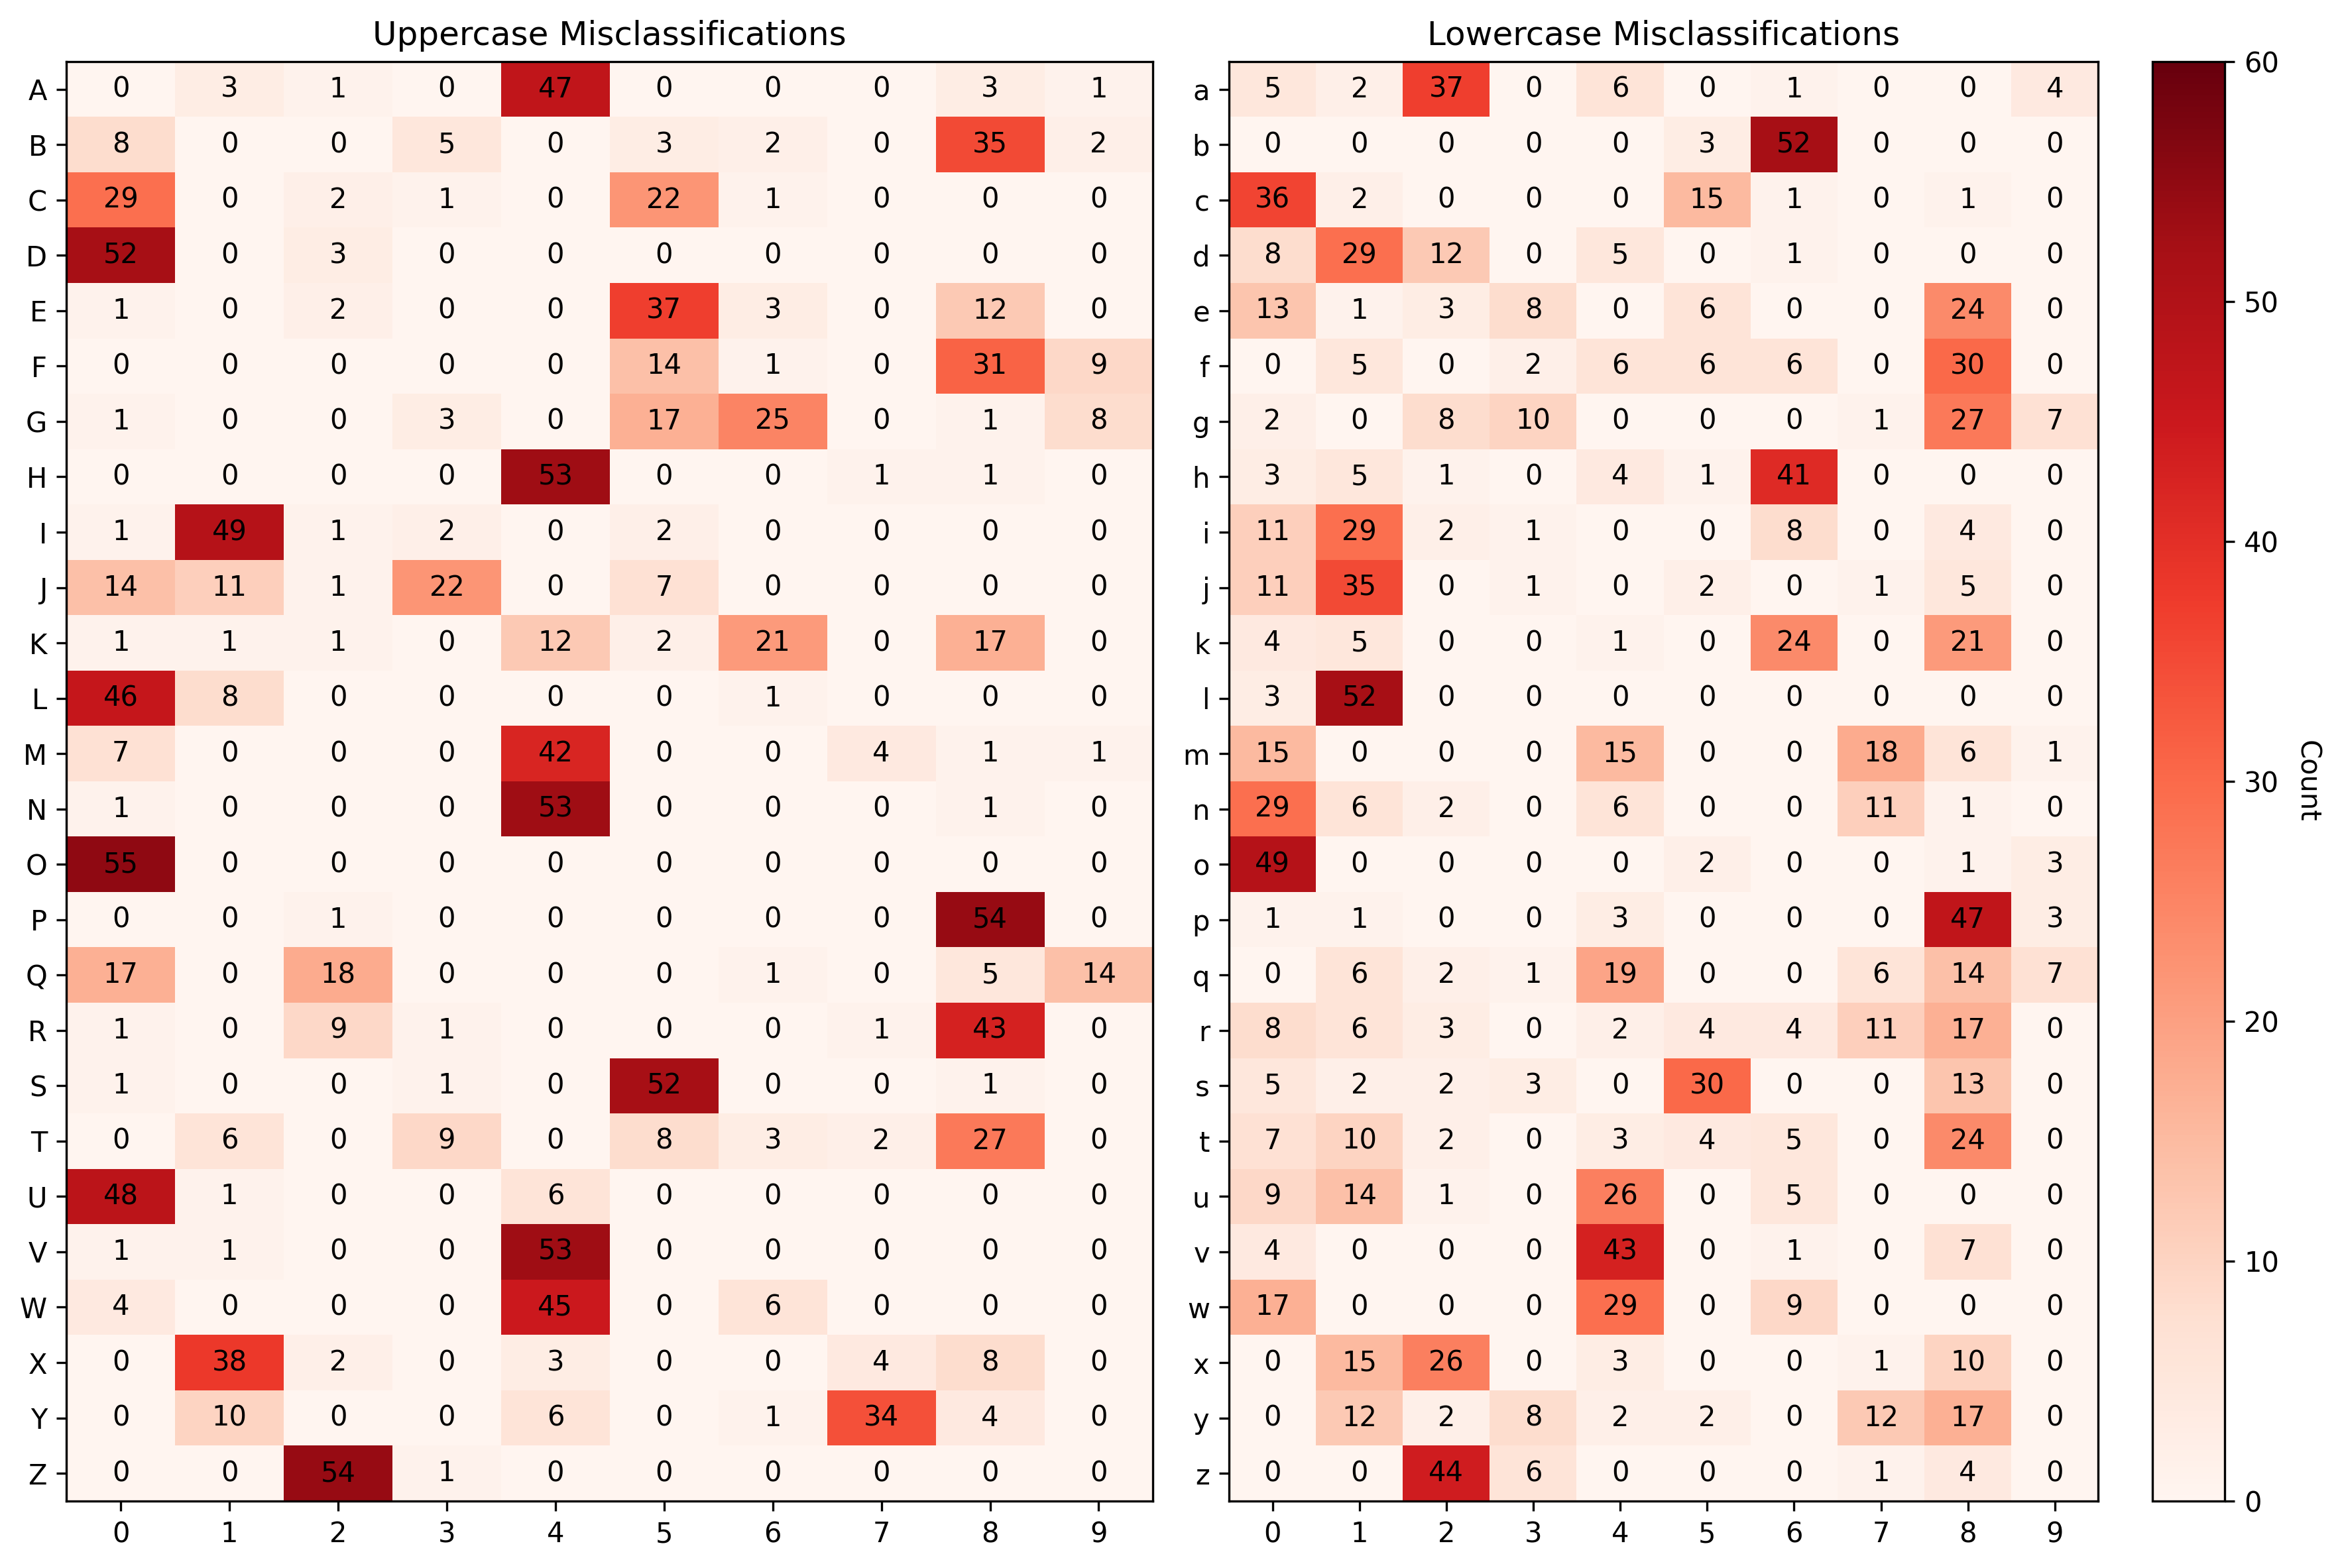
\includegraphics[width=0.99\columnwidth]{Figures/Results/HandwrittenCharacters/english_handwritten_characters_x_confusion_matrix.png}
    \caption{English Handwritten Alphabetic Characters nearest distance and example, and averages}
\label{fig:english_handwritten_characters_x_confusion_matrix}
\end{figure}

%%%%%%%%%%%%%%%%%%%%%%%%%%%%%
% SOFTMAX OUTPUT COMPARISON %
%%%%%%%%%%%%%%%%%%%%%%%%%%%%%

% function call (work in progress repo)
% plot_digit_averages(test_correct_predictions, test_incorrect_predictions, color1='lightgreen', color2='lightcoral', data="Testing Data")

% Figure \ref{fig:MNIST_Softmax_Averages_Training_appendix} shows the softmax output for correctly and incorrectly classified digits from the MNIST training dataset (60k examples) while Figure \ref{fig:english_handwritten_characters_digit_softmax_averages} shows the softmax output for correctly and incorrectly digits (alphabetic characters excluded) classifications of the English Handwritten Character MNISTified dataset (550 examples) no "0" or "4" digits where misclassified, hence the blank plots in the second row (misclassifications).
% % Figure \ref{fig:english_handwritten_characters_alphabetic_softmax_averages}

% \begin{figure*}[ht]
%     \centering
%     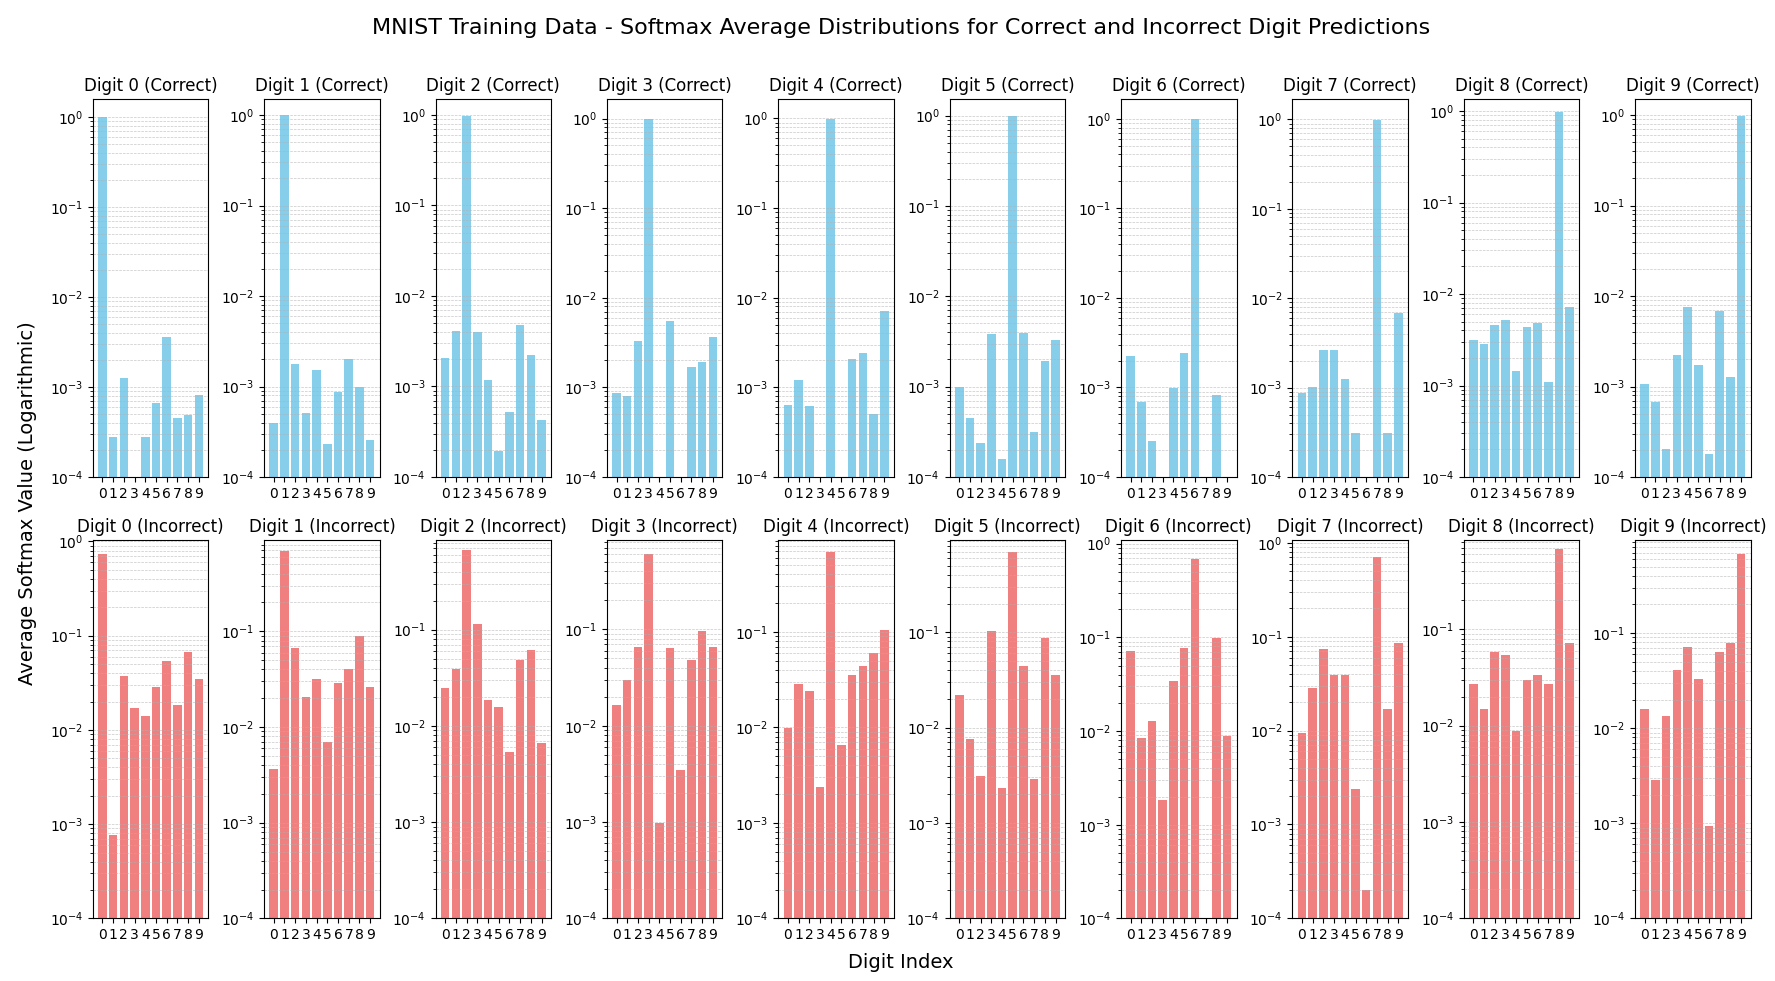
\includegraphics[width=0.99\textwidth]{Figures/Results/HandwrittenCharacters/MNIST_Softmax_Averages_Training.png}
%     \caption{Average Softmax Probabilities for Correctly and Incorrectly Classified Digits in the MNIST Training Dataset.}
%     \label{fig:MNIST_Softmax_Averages_Training_appendix}
% \end{figure*}

% \begin{figure*}[ht]
%     \centering
%     \includegraphics[width=0.99\textwidth]{Figures/Results/HandwrittenCharacters/MNIST_Softmax_Averages_Training.png}
%     \caption{Average Softmax Probabilities for Correctly and Incorrectly Classified Digits in the English Handwritten Characters Dataset (excludes alphabetical character predictions).}
%     \label{fig:english_handwritten_characters_digit_softmax_averages}
% \end{figure*}

% Generated by function call:
% plot_digit_averages(correct_digit_predictions, incorrect_digit_predictions, color1='skyblue', color2='lightcoral', data="English Handwritten Characters Digits Only", title= "Softmax Average Distributions for Correct and Incorrect Digit Predictions", filename="figures/english_handwritten_characters_digit_softmax_averages.png", save=True)
% # Saved average softmax outputs for correct and incorrect digit predictiions. figures/english_handwritten_characters_digit_softmax_averages.png

  
% \begin{figure*}[ht]
%     \centering
%     \includegraphics[width=0.99\textwidth]{Figures/Results/HandwrittenCharacters/english_handwritten_characters_digit_softmax_averages.png}
%     \caption{Average Softmax Probabilities for Correctly and Incorrectly Classified Digits in the English Handwritten Character MNISTified Dataset}
% \label{fig:english_handwritten_characters_digit_softmax_averages}
% \end{figure*}

% % plot_alphabetic_character_averages(alphabetic_predictions, color='lightcoral', data="English Handwritten Characters - Alphabetic Only", title="Softmax Average Distributions for Alphabetic Character Predictions", filename="figures/english_handwritten_characters_alphabetic_softmax_averages.png", save=True)
% % # Saved average softmax outputs for incorrect alphabetic character predictions. figures/english_handwritten_characters_alphabetic_softmax_averages.png

% \begin{figure*}[ht]
%     \centering
%     \includegraphics[width=0.99\textwidth]{Figures/Results/HandwrittenCharacters/english_handwritten_characters_alphabetic_softmax_averages.png}
%     \caption{Average Softmax Probabilities for Alphabetic Characters in the English Handwritten Character MNISTified Dataset}
% \label{fig:english_handwritten_characters_alphabetic_softmax_averages}
% \end{figure*}


% \subsection{MNIST, CIFAR-10 Training Dataset Entropy Comparison}

% \begin{figure}[ht]
%     \centering
%     \includegraphics[width=0.99\textwidth]{Figures/Results/HandwrittenCharacters/mnist_entropy_comparison.png}
%     \caption{MNIST entropy values for misclassified example from same class nearest to class centroid (cyan) and nearest misclassified example from different class to class centroid (red).}
% \label{fig:mnist_entropy_comparison}
% \end{figure}

% \begin{figure}[ht]
%     \centering
%     \includegraphics[width=0.99\textwidth]{Figures/Results/HandwrittenCharacters/cifar_vit_entropy_comparison.png}
%     \caption{CIFAR-10 entropy values for misclassified example from same class nearest to class centroid (cyan) and nearest misclassified example from different class to class centroid (red).}
% \label{fig:cifar_vit_entropy_comparison}
% \end{figure}


%\section{Training and Inference Results for Regression and Classification Models}
\section{Model Training and Inference Results}

We first trained regression models on datasets labeled with continuous steering values, corresponding to steering angles in the range -70 to 70 degrees, mapping to -1 to 1 steering units in CARLA simulator code. The trained models were evaluated in inference mode by allowing them to autonomously drive around the Town04 figure-of-eight circuit. During these runs, no lane invasions were observed; that is, the lateral deviation from the planned path, measured by the D MAE metric, remained below the defined threshold of 0.85 units. Following the procedure described in Section~\ref{methods:regression_classification}, these regression models were then adapted into classifiers by quantizing the continuous steering labels into discrete bins. The results for both the regression and classification models, during training and inference, are presented in the following sections.

\begin{figure}[h]
\centering
\includegraphics[width=0.99\textwidth]{Figures/Results/CNN_15_5_3_balanced_training.png}
\caption{Model Training and Evaluation Loss, from left to right, 15, 5 and 3-bin Classifier CNNs trained on balanced dataset.}
\label{fig:CNN_15_5_3_balanced_training}
\end{figure}

Figure~\ref{fig:CNN_15_5_3_balanced_training} presents typical training and validation loss curves for CNN classifiers trained on balanced datasets with 15, 5, and 3 quantized steering angle bins, shown left to right. The total number of samples for each dataset was approximately 153,000 (15-bin), 79,000 (5-bin), and 67,000 (3-bin).

The 15-bin model trained for the full 100 epochs without early stopping. Final training and validation losses were approximately 1.07 and 1.06, respectively, with accuracies around 48\%.



\subsection{Regression Models}
\begin{longtable}{@{}lllllll@{}}
\toprule
Model Name & Dataset & Train Loss & Eval Loss & MAE & O MAE & D MAE \\
\midrule
\endfirsthead
\toprule
Model Name & Dataset & Train Loss & Eval Loss & MAE & O MAE & D MAE \\
\midrule
\endhead
RegCNNCUFid & Cont Unbal w/ Fids & 0.0000 & 0.0000 & N/A & 0.0036 & 0.0461 \\
RegCNNCU & Continuous Unbal & N/A & N/A & N/A & 0.0033 & 0.0588 \\
RgrViTCU & Continuous Unbal & 0.0002 & 0.0001 & 0.0076 & 0.0076 & 0.0399 \\
\bottomrule
\caption{Regression Model Performance}
\label{results:table_regression_models}
\end{longtable}

Table~\ref{results:table_regression_models} reports the performance of three regression models trained on the continuous unbalanced dataset. The columns are as follows: Train Loss and Eval Loss refer to the mean squared error on the training and evaluation sets, respectively; MAE is the mean absolute error computed during training; O MAE is the mean absolute error calculated over the combined training and evaluation sets; and D MAE is the mean absolute lateral deviation of the simulated vehicle from the centerline, measured during autonomous driving in the Town04 figure-of-eight loop. Where N/A appears, the corresponding value was not recorded during training.

The RegCNNCUFid model incorporates fiducial markers as input and achieved a D MAE of 0.0461, with an O MAE of 0.0036. The RegCNNCU model, which uses the same architecture without fiducials, obtained a slightly lower O MAE (0.0033) but a higher D MAE (0.0588). The difference in D MAE between these two models is small and may be attributed to statistical noise, as both values remain well below the operational threshold of 0.85, beyond which lane invasion would occur.

The RgrViTCU model, based on a ViT architecture, yielded an O MAE of 0.0076 and the lowest D MAE among the three (0.0399). Since MAE values were not recorded for the CNN-based models, comparisons across all models using that column are not possible. All D MAE values are within the bounds of acceptable simulated driving behavior, and the differences observed do not approach the threshold of operational relevance.

\subsection{Classification Models}
\begin{longtable}{@{}llllllll@{}}
\toprule
Model Name & Dataset & T Acc & T Loss & V Acc & V Loss & O Acc & D MAE \\
\midrule
\endfirsthead
\toprule
Model Name & Dataset & T Acc & T Loss & V Acc & V Loss & O Acc & D MAE \\
\midrule
\endhead
ClsCNN3bB & 3-bin Bal & 83.16\% & 0.3797 & 83.02\% & 0.3808 & 83.36\% & 0.0365 \\
ClsCNN3bU & 3-bin Unbal & 86.97\% & 0.3129 & 87.14\% & 0.3110 & 87.36\% & 0.0466 \\
ClsCNN5bB & 5-bin Bal & 87.45\% & 0.3001 & 86.92\% & 0.2975 & 87.70\% & 0.0491 \\
ClsCNN5bU & 5-bin Unbal & 92.87\% & 0.1993 & 93.03\% & 0.1928 & 93.18\% & 0.0753 \\
ClsCNN15bB & 15-bin Bal & 48.01\% & 1.0744 & 47.81\% & 1.0598 & 48.01\% & 0.0162 \\
ClsCNN15bU & 15-bin Unbal & 73.76\% & 0.7241 & 75.34\% & 0.6839 & 75.11\% & 0.0194 \\
ClsViT3bB & 3-bin Bal & N/A & 0.1875 & 97.15\% & 0.0960 & 97.97\% & 0.0462 \\
ClsViT3bU & 3-bin Unbal & N/A & 0.2625 & 91.93\% & 0.2075 & 92.50\% & 0.0397 \\
ClsViT5bB & 5-bin Bal & N/A & 0.1317 & 97.54\% & 0.0766 & 97.77\% & 0.0454 \\
ClsViT5bU & 5-bin Unbal & N/A & 0.1985 & 94.05\% & 0.1590 & 94.97\% & 0.0666 \\
ClsViT15bB & 15-bin Bal & N/A & 0.4012 & 92.92\% & 0.1984 & 93.86\% & 0.0925 \\
ClsViT15bU & 15-bin Unbal & N/A & N/A & N/A & N/A & 76.55\% & 0.0844 \\
\bottomrule
\caption{Classification Model Performance: training and self-driving, with quantized balanced and unbalanced datasets. The first row shows data for a CNN classifier trained on a 3-bin dataset - steering angles -0.065 (-4.55 degrees), 0 and 0.065 (4.55 degrees). The training accuracy is 83.17\%, the training loss 0.3739, the validation accuracy 83.02\%, the validation loss 0.3808, the overall accuracy when training and validation datasets are combined is 83.36\%. The distance mean average error (DMAE)}
\label{results:classifier_models_results_table}
\end{longtable}

Table~\ref{results:classifier_models_results_table} presents the results for CNN and ViT models that were converted from regression models to perform classification, under three quantization schemes—3, 5, and 15 steering angle bins—and using either balanced or unbalanced datasets. The columns are as follows: T Acc and T Loss denote training accuracy and training loss; V Acc and V Loss are validation accuracy and validation loss; O Acc represents the overall accuracy across the full dataset (training and validation combined); and D MAE is the mean absolute error of the vehicle’s lateral deviation from the centerline. Entries marked N/A indicate that the corresponding values were not recorded during training. The D MAE values were computed through inference: after training, each model was deployed to drive autonomously around the Town04 figure-of-eight track, and its average distance from the intended trajectory was measured.

Among the CNN classifiers, ClsCNN5bU (trained on the unbalanced 5-bin dataset) achieved the highest overall accuracy (93.18\%), making it the best-performing CNN model. While its D MAE was slightly higher (0.0753), this remains well below the threshold (0.85 units) beyond which the vehicle would cross into an adjacent lane—meaning the deviation is not operationally significant and may be attributed to statistical noise. For the ViT models, ClsViT3bB (trained on the balanced 3-bin dataset) showed the strongest performance, with an overall accuracy of 97.97\% and a D MAE of 0.0462. In general, ViT models outperformed CNNs in both accuracy and driving precision, particularly on balanced datasets with coarser quantization. Given the low D MAE values across the board, most differences are unlikely to be practically significant in terms of simulated driving safety.

Overall Accuracy for CNN classifiers is consistently higher for models trained on unbalanced datasets, while the trend is inverted for ViT classifiers. This may be related to dataset sizes and network capacity, and is set as an investigative topic for future work.


\subsection{Best-Performing Classification Model Inference Results}

This section presents the results for the best performing models.


\textbf{ClsCNN5binUnbalanced}

\begin{table}[htbp]
\centering
\begin{tabular}{@{}lcccc@{}}
\toprule
\textbf{Class} & \textbf{Precision} & \textbf{Recall} & \textbf{F1-Score} & \textbf{Support} \\
\midrule
$-0.065$ & 0.80 & 0.36 & 0.50 & 401 \\
$-0.015$ & 0.85 & 0.97 & 0.90 & 5,843 \\
$\phantom{-}0.000$ & 0.98 & 0.95 & 0.97 & 15,839 \\
$\phantom{-}0.015$ & 0.90 & 0.96 & 0.93 & 3,972 \\
$\phantom{-}0.065$ & 0.87 & 0.57 & 0.69 & 936 \\
\midrule
\textbf{Macro Avg} & \textbf{0.88} & \textbf{0.76} & \textbf{0.80} & \textbf{26,991} \\
\bottomrule
\end{tabular}
\caption{Classification performance results for the ClsCNN5binUnbalanced model. The model achieved an overall accuracy of 93.18\% with a mean confidence of 0.9294 across 26,991 test images.}
\label{tab:clf_report_ClsCNN5binUnbalanced}
\end{table}

\begin{figure}[H]
\centering
\includegraphics[width=0.65\linewidth]{Figures/Results/cm_raw_ClsCNN5binUnbalanced.png}
\caption{ClsCNN5binUnbalanced model raw counts confusion matrix}
\label{fig:cm_raw_ClsCNN5binUnbalanced}
\end{figure}

\begin{figure}[H]
    \centering
    \includegraphics[width=1\linewidth]{Figures/Results/5_bins_cnn_softmax_dist_plot_unbalanced.png}
    \caption{Average Softmax Probabilities for Correctly and Incorrectly Classified Steering Angles in the 5 bin cnn unbalanced training Dataset.}
    \label{fig:5_bins_cnn_softmax_dist_unbalanced}
\end{figure}


\textbf{ClsViT3binBalanced}

\begin{table}[htbp]
\centering
\begin{tabular}{@{}lcccc@{}}
\toprule
\textbf{Class} & \textbf{Precision} & \textbf{Recall} & \textbf{F1-Score} & \textbf{Support} \\
\midrule
$-0.065$ & 0.98 & 1.00 & 0.99 & 22,460 \\
$\phantom{-}0.000$ & 1.00 & 0.94 & 0.97 & 22,460 \\
$\phantom{-}0.065$ & 0.96 & 1.00 & 0.98 & 22,460 \\
\midrule
\textbf{Macro Avg} & \textbf{0.98} & \textbf{0.98} & \textbf{0.98} & \textbf{67,380} \\
\bottomrule
\end{tabular}
\caption{Classification performance results for the ClsViT3binBalanced model. The model achieved an overall accuracy of 97.97\% with a mean confidence of 0.9765 across 67,380 test images.}
\label{tab:clf_report_ClsViT3binBalanced}
\end{table}

\begin{figure}[H]
\centering
\includegraphics[width=0.65\linewidth]{Figures/Results/cm_raw_ClsViT3binBalanced.png}
\caption{ClsViT3binBalanced model raw counts confusion matrix}
\label{fig:cm_raw_ClsViT3binBalanced}
\end{figure}

\begin{figure}[H]
    \centering
    \includegraphics[width=1\linewidth]{Figures/Results/3_bins_vit_softmax_dist_plot_balanced.png}
    \caption{Average Softmax Probabilities for Correctly and Incorrectly Classified Steering Angles in the 3 bin vit balanced training Dataset.}
    \label{fig:3_bins_vit_softmax_dist_balanced}
\end{figure}


\textbf{ClsViT5binBalanced}

\begin{table}[htbp]
\centering
\begin{tabular}{@{}lcccc@{}}
\toprule
\textbf{Class} & \textbf{Precision} & \textbf{Recall} & \textbf{F1-Score} & \textbf{Support} \\
\midrule
$-0.065$ & 0.99 & 1.00 & 1.00 & 15,839 \\
$-0.015$ & 0.96 & 0.99 & 0.97 & 15,839 \\
$\phantom{-}0.000$ & 0.99 & 0.95 & 0.97 & 15,839 \\
$\phantom{-}0.015$ & 1.00 & 0.95 & 0.97 & 15,839 \\
$\phantom{-}0.065$ & 0.96 & 1.00 & 0.98 & 15,839 \\
\midrule
\textbf{Macro Avg} & \textbf{0.98} & \textbf{0.98} & \textbf{0.98} & \textbf{79,195} \\
\bottomrule
\end{tabular}
\caption{Classification performance results for the ClsViT5binBalanced model. The model achieved an overall accuracy of 97.77\% with a mean confidence of 0.9779 across 79,195 test images.}
\label{tab:clf_report_ClsViT5binBalanced}
\end{table}

\begin{figure}[H]
\centering
\includegraphics[width=0.65\linewidth]{Figures/Results/cm_raw_ClsViT5binBalanced.png}
\caption{ClsViT5binBalanced model raw counts confusion matrix}
\label{fig:cm_raw_ClsViT5binBalanced}
\end{figure}

\begin{figure}[H]
    \centering
    \includegraphics[width=1\linewidth]{Figures/Results/5_bins_vit_softmax_dist_plot_balanced.png}
    \caption{Average Softmax Probabilities for Correctly and Incorrectly Classified Steering Angles in the 5 bin vit balanced training Dataset.}
    \label{fig:5_bins_vit_softmax_dist_balanced}
\end{figure}


\subsection{Additional Classification Model Inference Results}

This section presents the results for the remaining classification models that also showing sufficient prediction accuracy to safely steer the simulated vehicle around the figure-of-eight circuit.


\textbf{ClsCNN3binBalanced}

\begin{table}[htbp]
\centering
\begin{tabular}{@{}lcccc@{}}
\toprule
\textbf{Class} & \textbf{Precision} & \textbf{Recall} & \textbf{F1-Score} & \textbf{Support} \\
\midrule
$-0.065$ & 0.88 & 0.95 & 0.91 & 22,460 \\
$\phantom{-}0.000$ & 0.80 & 0.66 & 0.73 & 22,460 \\
$\phantom{-}0.065$ & 0.81 & 0.89 & 0.85 & 22,460 \\
\midrule
\textbf{Macro Avg} & \textbf{0.83} & \textbf{0.83} & \textbf{0.83} & \textbf{67,380} \\
\bottomrule
\end{tabular}
\caption{Classification performance results for the ClsCNN3binBalanced model. The model achieved an overall accuracy of 83.36\% with a mean confidence of 0.8312 across 67,380 test images.}
\label{tab:clf_report_ClsCNN3binBalanced}
\end{table}

\begin{figure}[H]
\centering
\includegraphics[width=0.65\linewidth]{Figures/Results/cm_raw_ClsCNN3binBalanced.png}
\caption{ClsCNN3binBalanced model raw counts confusion matrix}
\label{fig:cm_raw_ClsCNN3binBalanced}
\end{figure}

\begin{figure}[H]
    \centering
    \includegraphics[width=1\linewidth]{Figures/Results/3_bins_cnn_softmax_dist_plot_balanced.png}
    \caption{Average Softmax Probabilities for Correctly and Incorrectly Classified Steering Angles in the 3 bin cnn balanced training Dataset.}
    \label{fig:3_bins_cnn_softmax_dist_balanced}
\end{figure}


\textbf{ClsCNN3binUnbalanced}

\begin{table}[htbp]
\centering
\begin{tabular}{@{}lcccc@{}}
\toprule
\textbf{Class} & \textbf{Precision} & \textbf{Recall} & \textbf{F1-Score} & \textbf{Support} \\
\midrule
$-0.065$ & 0.61 & 0.28 & 0.38 & 1,422 \\
$\phantom{-}0.000$ & 0.89 & 0.97 & 0.93 & 22,460 \\
$\phantom{-}0.065$ & 0.79 & 0.42 & 0.55 & 3,059 \\
\midrule
\textbf{Macro Avg} & \textbf{0.76} & \textbf{0.56} & \textbf{0.62} & \textbf{26,941} \\
\bottomrule
\end{tabular}
\caption{Classification performance results for the ClsCNN3binUnbalanced model. The model achieved an overall accuracy of 87.36\% with a mean confidence of 0.8682 across 26,941 test images.}
\label{tab:clf_report_ClsCNN3binUnbalanced}
\end{table}

\begin{figure}[H]
\centering
\includegraphics[width=0.65\linewidth]{Figures/Results/cm_raw_ClsCNN3binUnbalanced.png}
\caption{ClsCNN3binUnbalanced model raw counts confusion matrix}
\label{fig:cm_raw_ClsCNN3binUnbalanced}
\end{figure}

\begin{figure}[H]
    \centering
    \includegraphics[width=1\linewidth]{Figures/Results/3_bins_cnn_softmax_dist_plot_unbalanced.png}
    \caption{Average Softmax Probabilities for Correctly and Incorrectly Classified Steering Angles in the 3 bin cnn unbalanced training Dataset.}
    \label{fig:3_bins_cnn_softmax_dist_unbalanced}
\end{figure}


\textbf{ClsCNN5binBalanced}

\begin{table}[htbp]
\centering
\begin{tabular}{@{}lcccc@{}}
\toprule
\textbf{Class} & \textbf{Precision} & \textbf{Recall} & \textbf{F1-Score} & \textbf{Support} \\
\midrule
$-0.065$ & 0.89 & 0.99 & 0.94 & 15,839 \\
$-0.015$ & 0.93 & 0.86 & 0.90 & 15,839 \\
$\phantom{-}0.000$ & 0.96 & 0.94 & 0.95 & 15,839 \\
$\phantom{-}0.015$ & 0.73 & 0.92 & 0.82 & 15,839 \\
$\phantom{-}0.065$ & 0.92 & 0.67 & 0.77 & 15,839 \\
\midrule
\textbf{Macro Avg} & \textbf{0.89} & \textbf{0.88} & \textbf{0.88} & \textbf{79,195} \\
\bottomrule
\end{tabular}
\caption{Classification performance results for the ClsCNN5binBalanced model. The model achieved an overall accuracy of 87.70\% with a mean confidence of 0.8762 across 79,195 test images.}
\label{tab:clf_report_ClsCNN5binBalanced}
\end{table}

\begin{figure}[H]
\centering
\includegraphics[width=0.65\linewidth]{Figures/Results/cm_raw_ClsCNN5binBalanced.png}
\caption{ClsCNN5binBalanced model raw counts confusion matrix}
\label{fig:cm_raw_ClsCNN5binBalanced}
\end{figure}

\begin{figure}[H]
    \centering
    \includegraphics[width=1\linewidth]{Figures/Results/5_bins_cnn_softmax_dist_plot_balanced.png}
    \caption{Average Softmax Probabilities for Correctly and Incorrectly Classified Steering Angles in the 5 bin cnn balanced training Dataset.}
    \label{fig:5_bins_cnn_softmax_dist_balanced}
\end{figure}


\textbf{ClsCNN15binBalanced}

\begin{table}[htbp]
\centering
\begin{tabular}{@{}lcccc@{}}
\toprule
\textbf{Class} & \textbf{Precision} & \textbf{Recall} & \textbf{F1-Score} & \textbf{Support} \\
\midrule
$-0.065$ & 0.37 & 0.43 & 0.40 & 10,199 \\
$-0.055$ & 0.22 & 0.27 & 0.24 & 10,199 \\
$-0.045$ & 0.34 & 0.39 & 0.36 & 10,199 \\
$-0.035$ & 0.00 & 0.00 & 0.00 & 10,199 \\
$-0.025$ & 0.40 & 0.60 & 0.48 & 10,199 \\
$-0.015$ & 0.46 & 0.36 & 0.40 & 10,199 \\
$-0.005$ & 0.77 & 0.95 & 0.85 & 10,199 \\
$\phantom{-}0.000$ & 0.85 & 0.94 & 0.89 & 10,199 \\
$\phantom{-}0.005$ & 0.54 & 0.81 & 0.65 & 10,199 \\
$\phantom{-}0.015$ & 0.51 & 0.12 & 0.20 & 10,199 \\
$\phantom{-}0.025$ & 0.46 & 0.40 & 0.43 & 10,199 \\
$\phantom{-}0.035$ & 0.44 & 0.54 & 0.48 & 10,199 \\
$\phantom{-}0.045$ & 0.48 & 0.31 & 0.38 & 10,199 \\
$\phantom{-}0.055$ & 0.38 & 0.77 & 0.51 & 10,199 \\
$\phantom{-}0.065$ & 0.85 & 0.31 & 0.45 & 10,199 \\
\midrule
\textbf{Macro Avg} & \textbf{0.47} & \textbf{0.48} & \textbf{0.45} & \textbf{152,985} \\
\bottomrule
\end{tabular}
\caption{Classification performance results for the ClsCNN15binBalanced model. The model achieved an overall accuracy of 48.01\% with a mean confidence of 0.4809 across 152,985 test images.}
\label{tab:clf_report_ClsCNN15binBalanced}
\end{table}

\begin{figure}[H]
\centering
\includegraphics[width=1\linewidth]{Figures/Results/cm_raw_ClsCNN15binBalanced.png}
\caption{ClsCNN15binBalanced model raw counts confusion matrix}
\label{fig:cm_raw_ClsCNN15binBalanced}
\end{figure}

\begin{figure}[H]
    \centering
    \includegraphics[width=1\linewidth]{Figures/Results/15_bins_cnn_softmax_dist_plot_balanced.png}
    \caption{Average Softmax Probabilities for Correctly and Incorrectly Classified Steering Angles in the 15 bin cnn balanced training Dataset.}
    \label{fig:15_bins_cnn_softmax_dist_balanced}
\end{figure}


\textbf{ClsCNN15binUnbalanced}

\begin{table}[htbp]
\centering
\begin{tabular}{@{}lcccc@{}}
\toprule
\textbf{Class} & \textbf{Precision} & \textbf{Recall} & \textbf{F1-Score} & \textbf{Support} \\
\midrule
$-0.065$ & 0.00 & 0.00 & 0.00 & 128 \\
$-0.055$ & 0.00 & 0.00 & 0.00 & 141 \\
$-0.045$ & 0.00 & 0.00 & 0.00 & 223 \\
$-0.035$ & 0.35 & 0.37 & 0.36 & 1,027 \\
$-0.025$ & 0.49 & 0.04 & 0.07 & 2,094 \\
$-0.015$ & 0.60 & 0.74 & 0.66 & 4,986 \\
$-0.005$ & 0.87 & 0.96 & 0.91 & 10,199 \\
$\phantom{-}0.000$ & 0.91 & 0.96 & 0.93 & 4,896 \\
$\phantom{-}0.005$ & 0.00 & 0.00 & 0.00 & 883 \\
$\phantom{-}0.015$ & 0.63 & 0.91 & 0.75 & 2,665 \\
$\phantom{-}0.025$ & 0.47 & 0.32 & 0.38 & 827 \\
$\phantom{-}0.035$ & 0.00 & 0.00 & 0.00 & 240 \\
$\phantom{-}0.045$ & 0.00 & 0.00 & 0.00 & 124 \\
$\phantom{-}0.055$ & 0.00 & 0.00 & 0.00 & 150 \\
$\phantom{-}0.065$ & 0.58 & 0.99 & 0.73 & 408 \\
\midrule
\textbf{Macro Avg} & \textbf{0.33} & \textbf{0.35} & \textbf{0.32} & \textbf{28,991} \\
\bottomrule
\end{tabular}
\caption{Classification performance results for the ClsCNN15binUnbalanced model. The model achieved an overall accuracy of 75.11\% with a mean confidence of 0.7495 across 28,991 test images.}
\label{tab:clf_report_ClsCNN15binUnbalanced}
\end{table}

\begin{figure}[H]
\centering
\includegraphics[width=1\linewidth]{Figures/Results/cm_raw_ClsCNN15binUnbalanced.png}
\caption{ClsCNN15binUnbalanced model raw counts confusion matrix}
\label{fig:cm_raw_ClsCNN15binUnbalanced}
\end{figure}

\begin{figure}[H]
    \centering
    \includegraphics[width=1\linewidth]{Figures/Results/15_bins_cnn_softmax_dist_plot_unbalanced.png}
    \caption{Average Softmax Probabilities for Correctly and Incorrectly Classified Steering Angles in the 15 bin cnn unbalanced training Dataset.}
    \label{fig:15_bins_cnn_softmax_dist_unbalanced}
\end{figure}


\textbf{ClsViT3binUnbalanced}

\begin{table}[htbp]
\centering
\begin{tabular}{@{}lcccc@{}}
\toprule
\textbf{Class} & \textbf{Precision} & \textbf{Recall} & \textbf{F1-Score} & \textbf{Support} \\
\midrule
$-0.065$ & 0.82 & 0.66 & 0.73 & 1,422 \\
$\phantom{-}0.000$ & 0.94 & 0.98 & 0.96 & 22,460 \\
$\phantom{-}0.065$ & 0.86 & 0.67 & 0.75 & 3,059 \\
\midrule
\textbf{Macro Avg} & \textbf{0.87} & \textbf{0.77} & \textbf{0.81} & \textbf{26,941} \\
\bottomrule
\end{tabular}
\caption{Classification performance results for the ClsViT3binUnbalanced model. The model achieved an overall accuracy of 92.50\% with a mean confidence of 0.9211 across 26,941 test images.}
\label{tab:clf_report_ClsViT3binUnbalanced}
\end{table}

\begin{figure}[H]
\centering
\includegraphics[width=0.65\linewidth]{Figures/Results/cm_raw_ClsViT3binUnbalanced.png}
\caption{ClsViT3binUnbalanced model raw counts confusion matrix}
\label{fig:cm_raw_ClsViT3binUnbalanced}
\end{figure}

\begin{figure}[H]
    \centering
    \includegraphics[width=1\linewidth]{Figures/Results/3_bins_vit_softmax_dist_plot_unbalanced.png}
    \caption{Average Softmax Probabilities for Correctly and Incorrectly Classified Steering Angles in the 3 bin vit unbalanced training Dataset.}
    \label{fig:3_bins_vit_softmax_dist_unbalanced}
\end{figure}


\textbf{ClsViT5binUnbalanced}

\begin{table}[htbp]
\centering
\begin{tabular}{@{}lcccc@{}}
\toprule
\textbf{Class} & \textbf{Precision} & \textbf{Recall} & \textbf{F1-Score} & \textbf{Support} \\
\midrule
$-0.065$ & 0.92 & 0.94 & 0.93 & 401 \\
$-0.015$ & 0.89 & 0.97 & 0.93 & 5,843 \\
$\phantom{-}0.000$ & 0.99 & 0.96 & 0.97 & 15,839 \\
$\phantom{-}0.015$ & 0.92 & 0.97 & 0.94 & 3,972 \\
$\phantom{-}0.065$ & 0.90 & 0.67 & 0.77 & 936 \\
\midrule
\textbf{Macro Avg} & \textbf{0.92} & \textbf{0.90} & \textbf{0.91} & \textbf{26,991} \\
\bottomrule
\end{tabular}
\caption{Classification performance results for the ClsViT5binUnbalanced model. The model achieved an overall accuracy of 94.97\% with a mean confidence of 0.9435 across 26,991 test images.}
\label{tab:clf_report_ClsViT5binUnbalanced}
\end{table}

\begin{figure}[H]
\centering
\includegraphics[width=0.65\linewidth]{Figures/Results/cm_raw_ClsViT5binUnbalanced.png}
\caption{ClsViT5binUnbalanced model raw counts confusion matrix}
\label{fig:cm_raw_ClsViT5binUnbalanced}
\end{figure}

\begin{figure}[H]
    \centering
    \includegraphics[width=1\linewidth]{Figures/Results/5_bins_vit_softmax_dist_plot_unbalanced.png}
    \caption{Average Softmax Probabilities for Correctly and Incorrectly Classified Steering Angles in the 5 bin vit unbalanced training Dataset.}
    \label{fig:5_bins_vit_softmax_dist_unbalanced}
\end{figure}


\textbf{ClsViT15binBalanced}

\begin{table}[htbp]
\centering
\begin{tabular}{@{}lcccc@{}}
\toprule
\textbf{Class} & \textbf{Precision} & \textbf{Recall} & \textbf{F1-Score} & \textbf{Support} \\
\midrule
$-0.065$ & 0.95 & 1.00 & 0.97 & 10,199 \\
$-0.055$ & 1.00 & 1.00 & 1.00 & 10,199 \\
$-0.045$ & 1.00 & 1.00 & 1.00 & 10,199 \\
$-0.035$ & 0.91 & 0.99 & 0.95 & 10,199 \\
$-0.025$ & 0.97 & 0.94 & 0.95 & 10,199 \\
$-0.015$ & 0.94 & 0.68 & 0.79 & 10,199 \\
$-0.005$ & 0.82 & 0.95 & 0.88 & 10,199 \\
$\phantom{-}0.000$ & 0.98 & 0.96 & 0.97 & 10,199 \\
$\phantom{-}0.005$ & 0.89 & 0.92 & 0.91 & 10,199 \\
$\phantom{-}0.015$ & 0.99 & 0.87 & 0.92 & 10,199 \\
$\phantom{-}0.025$ & 0.92 & 0.94 & 0.93 & 10,199 \\
$\phantom{-}0.035$ & 0.91 & 1.00 & 0.96 & 10,199 \\
$\phantom{-}0.045$ & 0.88 & 1.00 & 0.93 & 10,199 \\
$\phantom{-}0.055$ & 0.98 & 1.00 & 0.99 & 10,199 \\
$\phantom{-}0.065$ & 1.00 & 0.83 & 0.90 & 10,199 \\
\midrule
\textbf{Macro Avg} & \textbf{0.94} & \textbf{0.94} & \textbf{0.94} & \textbf{152,985} \\
\bottomrule
\end{tabular}
\caption{Classification performance results for the ClsViT15binBalanced model. The model achieved an overall accuracy of 93.86\% with a mean confidence of 0.9180 across 152,985 test images.}
\label{tab:clf_report_ClsViT15binBalanced}
\end{table}

\begin{figure}[H]
\centering
\includegraphics[width=1\linewidth]{Figures/Results/cm_raw_ClsViT15binBalanced.png}
\caption{ClsViT15binBalanced model raw counts confusion matrix}
\label{fig:cm_raw_ClsViT15binBalanced}
\end{figure}

\begin{figure}[H]
    \centering
    \includegraphics[width=1\linewidth]{Figures/Results/15_bins_vit_softmax_dist_plot_balanced.png}
    \caption{Average Softmax Probabilities for Correctly and Incorrectly Classified Steering Angles in the 15 bin vit balanced training Dataset.}
    \label{fig:15_bins_vit_softmax_dist_balanced}
\end{figure}


\textbf{ClsViT15binUnbalanced}

\begin{table}[htbp]
\centering
\begin{tabular}{@{}lcccc@{}}
\toprule
\textbf{Class} & \textbf{Precision} & \textbf{Recall} & \textbf{F1-Score} & \textbf{Support} \\
\midrule
$-0.065$ & 0.00 & 0.00 & 0.00 & 128 \\
$-0.055$ & 0.00 & 0.00 & 0.00 & 141 \\
$-0.045$ & 0.50 & 0.00 & 0.01 & 223 \\
$-0.035$ & 0.36 & 0.36 & 0.36 & 1,027 \\
$-0.025$ & 0.53 & 0.21 & 0.30 & 2,094 \\
$-0.015$ & 0.63 & 0.71 & 0.67 & 4,986 \\
$-0.005$ & 0.88 & 0.98 & 0.92 & 10,199 \\
$\phantom{-}0.000$ & 0.94 & 0.97 & 0.95 & 4,896 \\
$\phantom{-}0.005$ & 0.75 & 0.09 & 0.16 & 883 \\
$\phantom{-}0.015$ & 0.61 & 1.00 & 0.76 & 2,665 \\
$\phantom{-}0.025$ & 0.74 & 0.02 & 0.05 & 827 \\
$\phantom{-}0.035$ & 0.00 & 0.00 & 0.00 & 240 \\
$\phantom{-}0.045$ & 0.36 & 0.08 & 0.13 & 124 \\
$\phantom{-}0.055$ & 0.54 & 0.05 & 0.09 & 150 \\
$\phantom{-}0.065$ & 0.61 & 0.98 & 0.76 & 408 \\
\midrule
\textbf{Macro Avg} & \textbf{0.50} & \textbf{0.36} & \textbf{0.34} & \textbf{28,991} \\
\bottomrule
\end{tabular}
\caption{Classification performance results for the ClsViT15binUnbalanced model. The model achieved an overall accuracy of 76.55\% with a mean confidence of 0.7572 across 28,991 test images.}
\label{tab:clf_report_ClsViT15binUnbalanced}
\end{table}

\begin{figure}[H]
\centering
\includegraphics[width=1\linewidth]{Figures/Results/cm_raw_ClsViT15binUnbalanced.png}
\caption{ClsViT15binUnbalanced model raw counts confusion matrix}
\label{fig:cm_raw_ClsViT15binUnbalanced}
\end{figure}

\begin{figure}[H]
    \centering
    \includegraphics[width=1\linewidth]{Figures/Results/15_bins_vit_softmax_dist_plot_unbalanced.png}
    \caption{Average Softmax Probabilities for Correctly and Incorrectly Classified Steering Angles in the 15 bin vit unbalanced training Dataset.}
    \label{fig:15_bins_vit_softmax_dist_unbalanced}
\end{figure}


\textbf{ClsVLM3binUnbalanced}

\begin{table}[htbp]
\centering
\begin{tabular}{@{}lcccc@{}}
\toprule
\textbf{Class} & \textbf{Precision} & \textbf{Recall} & \textbf{F1-Score} & \textbf{Support} \\
\midrule
$-0.065$ & 0.50 & 0.19 & 0.27 & 1,422 \\
$\phantom{-}0.000$ & 0.86 & 0.99 & 0.92 & 22,460 \\
$\phantom{-}0.065$ & 0.91 & 0.17 & 0.28 & 3,059 \\
\midrule
\textbf{Macro Avg} & \textbf{0.76} & \textbf{0.45} & \textbf{0.49} & \textbf{26,941} \\
\bottomrule
\end{tabular}
\caption{Classification performance results for the ClsVLM3binUnbalanced model. The model achieved an overall accuracy of 85.08\% with a mean confidence of 0.9062 across 26,941 test images.}
\label{tab:clf_report_ClsVLM3binUnbalanced}
\end{table}

\begin{figure}[H]
\centering
\includegraphics[width=0.65\linewidth]{Figures/Results/cm_raw_ClsVLM3binUnbalanced.png}
\caption{ClsVLM3binUnbalanced model raw counts confusion matrix}
\label{fig:cm_raw_ClsVLM3binUnbalanced}
\end{figure}

\begin{figure}[H]
    \centering
    \includegraphics[width=1\linewidth]{Figures/Results/3_bins_vlm_softmax_dist_plot_unbalanced.png}
    \caption{Average Softmax Probabilities for Correctly and Incorrectly Classified Steering Angles in the 3 bin vlm unbalanced training Dataset.}
    \label{fig:3_bins_vlm_softmax_dist_unbalanced}
\end{figure}


\section{Classifier Models in Self-Driving Applications}

Channel-wise salt-and-pepper noise is applied to the RGB image by first calculating the noise probability $p = \text{intensity} \times 0.01$. A three-dimensional boolean mask $M$ with the same shape as the RGB image is then generated. Each element $M_{i,j,k}$ (for pixel $(i,j)$ and color channel $k \in \{R,G,B\}$) is set to True with probability $p$. The mask is applied to a copy of the original RGB image. Each True element in the mask corresponds to a color channel that gets corrupted. The original channel value $I_{i,j,k}$ is replaced with a new value $I'_{i,j,k} = \text{random}(0,1) \times 255$, which results in either 0 or 255. Since each of the three RGB channels is independently corrupted, a single pixel can exhibit any of the eight possible color combinations shown in Table \ref{tab:channel_wise_salt_pepper_colors}. These range from pure black (when all channels are set to 0) to pure white (when all channels are set to 255), with intermediate colors like red, green, blue, cyan, magenta, and yellow when channels are mixed.

\begin{longtable}{@{}llll@{}}
\toprule
R & G & B & Resulting Colour \\
\midrule
\endfirsthead
\toprule
R & G & B & Resulting Colour \\
\midrule
\endhead
0 & 0 & 0 & Black \\
0 & 0 & 255 & Blue \\
0 & 255 & 0 & Green \\
0 & 255 & 255 & Cyan \\
255 & 0 & 0 & Red \\
255 & 0 & 255 & Magenta \\
255 & 255 & 0 & Yellow \\
255 & 255 & 255 & White \\
\bottomrule
\caption{Possible pixel values and colours when channel-wise salt-and-pepper noise is applied independently to RGB channels}
\label{tab:channel_wise_salt_pepper_colors}
\end{longtable}


\begin{figure}[H]
    \centering
    \includegraphics[width=1.0\linewidth]{Figures/Results/experiment-247-251-255-3pc-10pc-50pc-rbg-pepper-noise-combined.jpg}
    \caption{CARLA simulator vehicle camera RGB image with 3\% (left), 10\% (middle) and 50\% channel-wise salt-and-pepper noise applied}
    \label{fig:experiment-247-251-255-3pc-10pc-50pc-rbg-pepper-noise-combined}
\end{figure}

Figure \ref{fig:experiment-247-251-255-3pc-10pc-50pc-rbg-pepper-noise-combined} shows images as would be presented to CNN (before preprocessing) and ViT networks (as is) for steering prediction. The image is generated by starting the simulation and saving one image. The images with channel-wise salt-and-pepper noise shown in the figure, were generated from left to right by experiments 247, 251 and 255.

\subsection{Self-driving Softmax Output Analysis}

 
\begin{figure}[H]
    \centering
    \includegraphics[width=1.0\linewidth]{Figures/Results/combined_cnn_5bin_vit_3bin_vit_5bin_noise_distance_metrics.png}
    \caption{Combined CNN 5 bin (left), ViT 3 bin (middle) and ViT 5 bin (right) noise levels by Average Path Distance (blue), Average Euclidean Distance (green), Average Bhattacharyya Distance (red), Average Histogram Intersection (cyan) and Average KL Divergence (purple). The pink band indicates noise levels where lane invasions occurred}
    \label{fig:combined_cnn_5bin_vit_3bin_vit_5bin_noise_distance_metrics}
\end{figure}

Figure \ref{fig:combined_cnn_5bin_vit_3bin_vit_5bin_noise_distance_metrics} shows the general trend that as noise levels increase, all distance metrics also increase, except Histogram Intersection, which has a maximum value of 1 when all RGB pixels are identical (0\% noise), and decreases as noise is added. As noise increases, the original and noisy images become dissimilar.
To obtain one data point in the plot, pepper noise is applied to the RGB image at 0, 10, 20, 30, 40 and 50\% pixel ratios. An average is taken for all predicted Softmax output Euclidean distances to centroids, across all classes (AvgED). An average distance is taken from the vehicle to the lane path across all path distance readings acquired during the simulation (AvgPD). The following averages are taken between the original image and the noisy image for all images generated by the simulation: Bhattacharyya Distance (AvgBD), Histogram Intersection (AvgHI), KL Divergence (AvgKL). Min-max normalization was applied to the averages being plotted, following the formula $x_{norm} = (x - x_{min}) / (x_{max} - x_{min})$, which scales all values to the range [0,1].

Bhattacharya Distance, Histogram Intersection and KL Divergence cannot be quantified in real world conditions because, unlike simulated scenarios, there is no "reference" image to be compared with. The metrics are still useful to confirm there exists a level of separation between the captured image and the image presented to the network, given noise. Distance to path cannot be quantified in real world conditions because the simulated path is determined by objects (waypoints) generated by the simulation, which do not exist in the same form (transform objects) in the real world. The key metric, determining if the model is "outside of its comfort zone", is the Average Euclidean Distance, The Euclidean distance between the network's Softmax output and the pre-computed class (discretized steering angles) centroids is the only quantity that can be computed in the wild.
The pink region of the plots mark the occurrence of lane invasions. For example, the left hand side plot for the CNN trained on 5 bin quantized (-0.065, -0.015, 0.0000, 0.0150 and 0.0650 steering angle classes) balanced data: , presented lane invasions where at 40\% noise, where 40\% noise would approximately correspond to the right hand side image in Figure \ref{fig:combined_cnn_5bin_vit_3bin_vit_5bin_noise_distance_metrics}. 

Table \ref{tab:experiment_stats_common_0_10_20_30_40_50} presents results for experiments that were common to the three models tested - the best performing CNN model (5 bin-quantized unbalanced-dataset, 93.18\% overall accuracy) the corresponding best performing 5 bin-quantized balanced-dataset ViT model (97.77\% overall accuracy) and the best performing model overall, the ViT 3 bin-quantized balanced-dataset model (97.97\% overall accuracy).

Further, Table \ref{tab:experiment_stats_common_0_10_20_30_40_50} presents the original values used to compute the plots in Figure \ref{fig:combined_cnn_5bin_vit_3bin_vit_5bin_noise_distance_metrics}. The bold font in consecutive rows, column AvgED, shows where a lane invasion was observed. For example, in experiment 240, the CNN 5 bin model steering, with front facing camera images subject to 40\% noise, lead to a lane invasion (column LI presenting value T). The lane invasion lead to the simulation being stopped at frame count 10133 (FrCnt). The average distance to the optimal trajectory path (AvrPD) was recorded at 0.1080 units of distance for the all distance to path readings (PDCont), the average Euclidean distance to predicted class centroid (AvgED) was recorded at 0.6257 (across all predictions, corresponding in number to the frame count FrCnt). In general the average Bhattacharya Distance (AvgBD) and KL Divergence (AvgKL) tend to increase with noise, while Histogram Intersection (AvgHI) tends to decrease with noise.
The average Euclidean distance to the predicted class centroid (AvgED) tend to increase with noise. 
Since the aim is to ensure autonomous system safety, a prediction, under the experimental parameters, can be considered safe when no lane invasion occurs. Therefore, we make note of the nearest average Euclidean distance to predicted class centroid, where a lane invasion occurred while the simulated vehicle was steering with predictions from the CNN 5 bin classifier. The nearest average (lowest value) was observed in experiment 241, 0.6061. We note that there are higher averages - experiment 239, 30\% noise, 0.6828 - where lane invasions did not occur. Our choice for threshold for the CNN 5 bin model should be between 0.6061 and 0.2829 average Euclidean distance from the class softmax outputs to the predicted class centroids. In other words, the threshold should be placed between the highest AvgED value where a lane invasion did not occur and the lowest AvgED value where a lane invasion occurred, for a given model. We highlight the values in boldface in Table \ref{tab:experiment_stats_common_0_10_20_30_40_50}. In short, for the CNN 5 bin classifier, the threshold should be placed between 0.2892 and 0.6061.

Based on the common results for noise levels 0, 10, 20, 30, 40 and 50\%, and applying the same constraints, the ViT 3 bin threshold should be placed between 0.0437 and 0.1530. In practice, the ViT 3 bin model presented lane invasions at lower noise levels compared to the CNN 5 bin model, leading to shorter intervals. 
We present the full results in Table \ref{tab:experiment_stats}.


\begin{longtable}{@{}cllrrrrrrrrrc@{}}
\toprule
Exp & Net & Bins & Noise & AvgPD & PDCnt & AvgED & AvgBD & AvgHI & AvgKL & FrCnt & LI \\
\midrule
\endfirsthead
\toprule
Exp & Net & Bins & Noise & AvgPD & PDCnt & AvgED & AvgBD & AvgHI & AvgKL & FrCnt & LI \\
\midrule
\endhead
262 & CNN & 5 & 0 & 0.0600 & 1032 & 0.2634 & 0.0706 & 0.8091 & 0.1016 & 19749 & F \\
237 & CNN & 5 & 10 & 0.0529 & 1032 & 0.1787 & 0.0493 & 0.8681 & 0.0699 & 20534 & F \\
238 & CNN & 5 & 20 & 0.0160 & 1032 & \textbf{0.2892} & 0.0829 & 0.7765 & 0.0957 & 22356 & F \\
239 & CNN & 5 & 30 & 0.0592 & 1032 & 0.6828 & 0.3588 & 0.4053 & 0.3785 & 22375 & F \\
240 & CNN & 5 & 40 & 0.1080 & 473 & 0.6257 & 0.2982 & 0.4621 & 0.3154 & 10133 & T \\
241 & CNN & 5 & 50 & 0.2871 & 473 & \textbf{0.6061} & 0.2803 & 0.4861 & 0.2938 & 10550 & T \\
263 & ViT & 3 & 0 & 0.1127 & 1032 & \textbf{0.0437} & 0.0120 & 0.9676 & 0.0296 & 8736 & F \\
251 & ViT & 3 & 10 & 0.1631 & 17 & \textbf{0.1530} & 0.0362 & 0.8898 & 0.0443 & 130 & T \\
252 & ViT & 3 & 20 & 0.1997 & 15 & 0.2156 & 0.0553 & 0.8423 & 0.0666 & 108 & T \\
253 & ViT & 3 & 30 & 0.2552 & 12 & 0.3234 & 0.0872 & 0.7623 & 0.1044 & 90 & T \\
254 & ViT & 3 & 40 & 0.3238 & 8 & 0.4130 & 0.1199 & 0.6914 & 0.1422 & 58 & T \\
255 & ViT & 3 & 50 & 0.3374 & 5 & 0.5513 & 0.1811 & 0.5798 & 0.2120 & 34 & T \\
266 & ViT & 5 & 0 & 0.0753 & 1032 & \textbf{0.1156} & 0.0330 & 0.9165 & 0.0409 & 4358 & F \\
256 & ViT & 5 & 10 & 0.1076 & 39 & \textbf{0.4051} & 0.1599 & 0.6660 & 0.1720 & 164 & T \\
257 & ViT & 5 & 20 & 0.2266 & 25 & 0.5415 & 0.2488 & 0.5440 & 0.2618 & 101 & T \\
258 & ViT & 5 & 30 & 0.1537 & 30 & 0.5588 & 0.2605 & 0.5234 & 0.2761 & 120 & T \\
259 & ViT & 5 & 40 & 0.1538 & 40 & 0.6238 & 0.3167 & 0.4615 & 0.3307 & 157 & T \\
260 & ViT & 5 & 50 & 0.2823 & 29 & 0.7479 & 0.4470 & 0.3418 & 0.4576 & 114 & T \\
\bottomrule
\caption{Common experiment results for noise levels 0\%, 10\%, 20\%, 30\%, 40\%, and 50\% across three models: CNN 5-bin (unbalanced dataset, 93.18\% accuracy), ViT 5-bin (balanced dataset, 97.77\% accuracy), and ViT 3-bin (balanced dataset, 97.97\% accuracy). The table reports metrics including average path deviation (AvgPD), path deviation count (PDCnt) - this is the number of times in the simulation the distance from the vehicle from the path was computed, average Euclidean distance to predicted class centroid (AvgED, bolded where lane invasions occurred), average Bhattacharyya distance (AvgBD), average histogram intersection (AvgHI), average KL divergence (AvgKL), frame count (FrCnt), and lane invasion status (LI, T for true, F for false). These metrics underpin the plots in Figure~\ref{fig:combined_cnn_5bin_vit_3bin_vit_5bin_noise_distance_metrics}. For safety, thresholds for AvgED are proposed to avoid lane invasions: for CNN 5-bin, between 0.2892 (highest safe) and 0.6061 (lowest unsafe); for ViT 3-bin, between 0.0437 and 0.1530; for ViT 5-bin, between 0.1156 and 0.4051.}
\label{tab:experiment_stats_common_0_10_20_30_40_50}
\end{longtable}

\subsection{Setting Distance-to-Centroid Thresholds}

The threshold selection methodology for preventing lane invasions applies framework described in the contributions, which demonstrates that Euclidean distance between softmax outputs and class centroids serves as a proxy for prediction confidence. The work establishes that setting distance thresholds based on distances from incorrect predictions to class centroids enables systems to identify unreliable predictions and defer judgment.

In our autonomous driving implementation, this translates to safety thresholds: when steering predictions exceed the distance threshold to their class centroid, the system should reject the prediction as potentially unsafe. The threshold ranges in Table \ref{tab:experiment_stats_common_0_10_20_30_40_50} represent conservative boundaries derived from the minimum distance observed for lane invasions in our simulated scenarios. 

\begin{longtable}{@{}cllrrrrrrrrrc@{}}
\toprule
Exp & Net & Bins & Noise & AvgPD & PDCnt & AvgED & AvgBD & AvgHI & AvgKL & FrCnt & LI \\
\midrule
\endfirsthead
\toprule
Exp & Net & Bins & Noise & AvgPD & PDCnt & AvgED & AvgBD & AvgHI & AvgKL & FrCnt & LI \\
\midrule
\endhead
262 & CNN & 5 & 0 & 0.0600 & 1032 & 0.2634 & 0.0706 & 0.8091 & 0.1016 & 19749 & F \\
237 & CNN & 5 & 10 & 0.0529 & 1032 & 0.1787 & 0.0493 & 0.8681 & 0.0699 & 20534 & F \\
238 & CNN & 5 & 20 & 0.0160 & 1032 & 0.2892 & 0.0829 & 0.7765 & 0.0957 & 22356 & F \\
239 & CNN & 5 & 30 & 0.0592 & 1032 & 0.6828 & 0.3588 & 0.4053 & 0.3785 & 22375 & F \\
240 & CNN & 5 & 40 & 0.1080 & 473 & 0.6257 & 0.2982 & 0.4621 & 0.3154 & 10133 & T \\
241 & CNN & 5 & 50 & 0.2871 & 473 & 0.6061 & 0.2803 & 0.4861 & 0.2938 & 10550 & T \\
242 & CNN & 5 & 55 & 0.3853 & 189 & 0.5933 & 0.2715 & 0.5011 & 0.2823 & 4146 & T \\
243 & CNN & 5 & 60 & 0.3105 & 18 & 0.5292 & 0.2141 & 0.5533 & 0.2342 & 369 & T \\
263 & ViT & 3 & 0 & 0.1127 & 1032 & 0.0437 & 0.0120 & 0.9676 & 0.0296 & 8736 & F \\
245 & ViT & 3 & 1 & 0.1805 & 217 & 0.1063 & 0.0255 & 0.9232 & 0.0339 & 930 & T \\
246 & ViT & 3 & 2 & 0.1163 & 34 & 0.0601 & 0.0148 & 0.9545 & 0.0204 & 144 & T \\
247 & ViT & 3 & 3 & 0.1087 & 34 & 0.0617 & 0.0141 & 0.9537 & 0.0184 & 145 & T \\
248 & ViT & 3 & 4 & 0.1215 & 34 & 0.0666 & 0.0140 & 0.9507 & 0.0183 & 144 & T \\
249 & ViT & 3 & 5 & 0.1360 & 33 & 0.0697 & 0.0149 & 0.9488 & 0.0191 & 140 & T \\
250 & ViT & 3 & 7 & 0.1276 & 34 & 0.0727 & 0.0145 & 0.9471 & 0.0185 & 271 & T \\
251 & ViT & 3 & 10 & 0.1631 & 17 & 0.1530 & 0.0362 & 0.8898 & 0.0443 & 130 & T \\
252 & ViT & 3 & 20 & 0.1997 & 15 & 0.2156 & 0.0553 & 0.8423 & 0.0666 & 108 & T \\
253 & ViT & 3 & 30 & 0.2552 & 12 & 0.3234 & 0.0872 & 0.7623 & 0.1044 & 90 & T \\
254 & ViT & 3 & 40 & 0.3238 & 8 & 0.4130 & 0.1199 & 0.6914 & 0.1422 & 58 & T \\
255 & ViT & 3 & 50 & 0.3374 & 5 & 0.5513 & 0.1811 & 0.5798 & 0.2120 & 34 & T \\
266 & ViT & 5 & 0 & 0.0753 & 1032 & 0.1156 & 0.0330 & 0.9165 & 0.0409 & 4358 & F \\
256 & ViT & 5 & 10 & 0.1076 & 39 & 0.4051 & 0.1599 & 0.6660 & 0.1720 & 164 & T \\
257 & ViT & 5 & 20 & 0.2266 & 25 & 0.5415 & 0.2488 & 0.5440 & 0.2618 & 101 & T \\
258 & ViT & 5 & 30 & 0.1537 & 30 & 0.5588 & 0.2605 & 0.5234 & 0.2761 & 120 & T \\
259 & ViT & 5 & 40 & 0.1538 & 40 & 0.6238 & 0.3167 & 0.4615 & 0.3307 & 157 & T \\
260 & ViT & 5 & 50 & 0.2823 & 29 & 0.7479 & 0.4470 & 0.3418 & 0.4576 & 114 & T \\
261 & ViT & 5 & 60 & 0.3657 & 8 & 0.7627 & 0.4828 & 0.3254 & 0.4818 & 34 & T \\
\bottomrule
\caption{Experiment Statistics with Lane Invasion, full results}
\label{tab:experiment_stats}
\end{longtable}

Table \ref{tab:youtube_links} presents links to video captures of experiments where lane invasions did and did not occur (column LI showing values T and F respectively). The simulation is generated as described in Section \ref{methods:carla}.

\begin{longtable}{@{}clcrcc@{}}
\toprule
Exp & Net & Bins & Noise & LI & YouTube \\
\midrule
\endfirsthead
\toprule
Exp & Net & Bins & Noise & LI & YouTube \\
\midrule
\endhead
262 & CNN & 5 & 0 & F & \href{https://youtu.be/vhbmxwMlZfk}{Video} \\
237 & CNN & 5 & 10 & F & \href{https://youtu.be/3Zsny4NM_NQ}{Video} \\
%238 & CNN & 5 & 20 & F & \href{https://youtu.be/RaCVAlwBQlQ}{Video} \\
239 & CNN & 5 & 30 & F & \href{https://youtu.be/CzJlbYX0CnQ}{Video} \\
240 & CNN & 5 & 40 & T & \href{https://youtu.be/FVlpiNw26J8}{Video} \\
241 & CNN & 5 & 50 & T & \href{https://youtu.be/O74AcmhYF2Y}{Video} \\
242 & CNN & 5 & 55 & T & \href{https://youtu.be/Ui-xJKEpXRs}{Video} \\
263 & ViT & 3 & 0 & F & \href{https://youtu.be/NvsoVrbx9xA}{Video} \\
255 & ViT & 3 & 50 & T & \href{https://youtu.be/e17e30eX0Rg}{Video} \\
266 & ViT & 5 & 0 & F & \href{https://youtu.be/d1YI4Eko4JE}{Video} \\
261 & ViT & 5 & 60 & T & \href{https://youtu.be/OyENq7Xe88Q}{Video} \\
270 & VLM DS & 3 & 0 & T & \href{https://youtu.be/HbAAoUBcfDw}{Video} \\
288 & VLM Qwen & 3 & 0 & T & \href{https://youtu.be/tY1LgKakAZ4}{Video} \\
\bottomrule
\caption{Experiments with YouTube Video Links. Experiments 270 and 288 for the Vision Language Models}
\label{tab:youtube_links}
\end{longtable}

Figure \ref{fig:Exp239-30pc-noise-CNN-5-bin-bal-youtube.png} shows a screen shot of the experiment 239 video capture as uploaded to YouTube (link given in table \ref{tab:youtube_links}). In the background and prominent on the left is the terminal screen with debug information about the nearest waypoints that define the route path, and the computed perpendicular distance to the path once the simulated vehicle is less than 1.5 units of distance to the next waypoint.
Resized on the bottom left is the CARLA simulator viewport.
The CARLA simulation captures RGB images (640x480) using a vehicle-mounted camera, managed by the CarlaSteering class. The process\_image method converts raw BGR data to RGB, storing it in self.image\_queue as self.original\_img. The preprocess\_image method crops (top/bottom) and resizes the image, converts it to YUV (self.pre\_noise\_yuv), applies pepper noise (0\%-100\% intensity) to RGB if specified, then converts the noisy RGB to YUV (self.post\_noise\_yuv). The noisy YUV is transposed for neural network input (self.preprocessed\_img) and returned as a PyTorch tensor. The display\_images method resizes self.original\_img and self.preprocessed\_img (YUV) to 264px height, creates a side-by-side canvas (width: original\_width + image\_width + 20px), and displays it using OpenCV (cv2.imshow) with labels "Original Camera Feed" and "Neural Network Input (YUV)". The DistanceMetrics object computes Bhattacharyya, Histogram Intersection, and KL Divergence between self.pre\_noise\_yuv and self.post\_noise\_yuv, stored in self.prediction\_data.

\begin{figure}[h]
    \centering
    \includegraphics[width=0.75\textwidth]{Figures/Results/Exp239-30pc-noise-CNN-5-bin-bal-youtube.png}
    \caption{Experiment 239 YouTube video screenshot capture}
    \label{fig:Exp239-30pc-noise-CNN-5-bin-bal-youtube.png}
\end{figure}


\subsection{Euclidean Distance to Centroids Preceding a Lane Invasion}
\label{res:ed_centroids_preceding_lane_invasion}

We are interested in observing if the Euclidean Distance of a self-driving network softmax output to the predicted class centroid "spikes", that is presents a sharp increase, before a lane invasion is about to occur. As previously discussed, a lane invasion is defined when a vehicle's perpendicular distance to middle of the lane path is found to be greater than 0.85 units. 

Table \ref{tab:li_ed_comparison} presents average network softmax output Euclidean distance to class centroids for the last 10, 20 and 30 predictions (noting exactly one prediction is generated for every frame), where a lane invasion has occurred. Column \textbf{Exp} (integer) is the experiment ID , \textbf{Net} (string) is the network, \textbf{Noise} (integer percentage) is the percentage of pepper noise applied to the original vehicle's front facing camera image, \textbf{AvgED} (float) is the overall average Euclidean distance to predicted class centroid, \textbf{AvgED-LI-10} (float), \textbf{AvgED-LI-20} (float)  and \textbf{AvgED-LI-30} (float) is the same average, over the last 10, 20 and 30 predictions respectively, \textbf{FrCnt} (integer) is the frame count (number of predictions/frames) and \textbf{LI} (boolean) is the lane invasion boolean flag taking value T (true) when a lane invasion has occurred. Lane invasions occurred in all experiments reported in the table.


\begin{longtable}{@{}clcrrrrrcc@{}}
\toprule
Exp & Net & Bins & Noise & AvgED & AvgED-LI-10 & AvgED-LI-20 & AvgED-LI-30 & FrCnt & LI \\
\midrule
\endfirsthead
\toprule
Exp & Net & Bins & Noise & AvgED & AvgED-LI-10 & AvgED-LI-20 & AvgED-LI-30 & FrCnt & LI \\
\midrule
\endhead
240 & CNN & 5 & 40 & 0.6257 & 0.5616 & 0.5610 & 0.5631 & 10133 & T \\
241 & CNN & 5 & 50 & 0.6061 & 0.6215 & 0.6219 & 0.6273 & 10550 & T \\
242 & CNN & 5 & 55 & 0.5933 & 0.5135 & 0.5088 & 0.5192 & 4146 & T \\
243 & CNN & 5 & 60 & 0.5292 & 0.6206 & 0.6046 & 0.6041 & 369 & T \\
245 & ViT & 3 & 1 & 0.1063 & 0.3066 & 0.2268 & 0.1737 & 930 & T \\
246 & ViT & 3 & 2 & 0.0601 & 0.3339 & 0.2960 & 0.2088 & 144 & T \\
247 & ViT & 3 & 3 & 0.0617 & 0.3593 & 0.2924 & 0.2042 & 145 & T \\
248 & ViT & 3 & 4 & 0.0666 & 0.2934 & 0.2738 & 0.1912 & 144 & T \\
249 & ViT & 3 & 5 & 0.0697 & 0.2580 & 0.2349 & 0.1636 & 140 & T \\
250 & ViT & 3 & 7 & 0.0727 & 0.1358 & 0.2280 & 0.2591 & 271 & T \\
251 & ViT & 3 & 10 & 0.1530 & 0.3659 & 0.4113 & 0.3822 & 130 & T \\
252 & ViT & 3 & 20 & 0.2156 & 0.5062 & 0.4387 & 0.3874 & 108 & T \\
253 & ViT & 3 & 30 & 0.3234 & 0.5033 & 0.4594 & 0.4011 & 90 & T \\
254 & ViT & 3 & 40 & 0.4130 & 0.3171 & 0.3938 & 0.4251 & 58 & T \\
255 & ViT & 3 & 50 & 0.5513 & 0.5834 & 0.5582 & 0.5628 & 34 & T \\
256 & ViT & 5 & 10 & 0.4051 & 0.5901 & 0.5571 & 0.4842 & 164 & T \\
257 & ViT & 5 & 20 & 0.5415 & 0.6642 & 0.6754 & 0.6732 & 101 & T \\
258 & ViT & 5 & 30 & 0.5588 & 0.6995 & 0.6623 & 0.6020 & 120 & T \\
259 & ViT & 5 & 40 & 0.6238 & 0.7005 & 0.6296 & 0.6227 & 157 & T \\
260 & ViT & 5 & 50 & 0.7479 & 0.7522 & 0.7637 & 0.7658 & 114 & T \\
261 & ViT & 5 & 60 & 0.7627 & 0.7671 & 0.7598 & 0.7571 & 34 & T \\
\bottomrule
\caption{Comparison of Overall and Last 10, 20, 30 Predictions Euclidean Distance to Predicted Class Centroids for Experiments where Lane Invasion Occurred}
\label{tab:li_ed_comparison}
\end{longtable}


In Table \ref{tab:li_ed_comparison}, the average Euclidean distance to predicted class centroid for the last 10, 20 and 30 predictions is examined for experiments that resulted in lane invasions. 

Table \ref{tab:experiment_stats} reports key metrics—average path distance (AvgPD), Euclidean distance (AvgED), Bhattacharyya distance (AvgBD), histogram intersection (AvgHI), KL divergence (AvgKL), frame count (FrCnt), and lane invasion status (LI)—across 27 experiments. Lane invasions (LI = T) occurred at noise levels of 40–60\% for CNN (5 bins) and 1–60\% for ViT (3/5 bins), with increased AvgED and AvgKL signaling prediction instability. Figure \ref{fig:combined_cnn_5bin_vit_3bin_vit_5bin_noise_distance_metrics} show normalized metrics against noise (0, 10, 20, 30, 40, 50\%), with shaded regions indicating LI = T thresholds (e.g., Noise 40 for CNN, 5 bins; Noise 10 for ViT, 3/5 bins), highlighting metric degradation during invasions. Table\ref{tab:youtube_links} provides YouTube video links for select experiments (e.g., Exp 261, ViT, 5 bins, 60\% noise), showing evidence of lane invasions. Table\ref{tab:li_ed_comparison} analyzes 21 LI = T experiments (Exps 240–243, 245–261), comparing the overall average Euclidean distance (AvgED) to averages for the last 10, 20, and 30 predictions (AvgED-LI-10, AvgED-LI-20, AvgED-LI-30), alongside noise and frame counts. For CNN (5 bins), AvgED-LI-10 varies relative to AvgED (e.g., 0.5616 vs. 0.6257 for Exp 240; 0.6215 vs. 0.6061 for Exp 241), with AvgED-LI-20 and AvgED-LI-30 showing similar variability (e.g., 0.5610, 0.5631 for Exp 240; 0.6046, 0.6041 for Exp 243), suggesting inconsistent prediction errors near invasions. For ViT (3 bins), AvgED-LI-10 is often higher than AvgED at low noise (e.g., 0.3066 vs. 0.1063 for Exp 245, Noise 1\%), but AvgED-LI-20 and AvgED-LI-30 decrease (e.g., 0.2268, 0.1737), indicating transient errors in the final 10 frames that stabilize over longer windows. At higher noise (e.g., Exp 252, Noise 20\%), AvgED-LI-10 remains high (0.5062), with AvgED-LI-20 and AvgED-LI-30 slightly lower (0.4387, 0.3874), suggesting sustained degradation. For ViT (5 bins), AvgED-LI-10 consistently exceeds AvgED (e.g., 0.6642 vs. 0.5415 for Exp 257, Noise 20\%), with AvgED-LI-20 and AvgED-LI-30 varying (e.g., 0.6754, 0.6732 for Exp 257; 0.7598, 0.7571 for Exp 261), reflecting persistent prediction errors. These findings highlight ViT’s greater sensitivity to noise, with earlier lane invasions (Noise 1\% for 3 bins) and larger prediction errors in the final 10–30 frames compared to CNN (Noise 40\%), critical for assessing safety in noisy environments.

\section{Vision-Language Models for Scene Understanding}
\label{sec:vlm_scene_understanding}

This section evaluates two vision-language models (VLMs), DeepSeek-VL-1.3B-Chat and Qwen2-VL-2B-Instruct, for scene understanding in a self-driving task using the CARLA simulator. The task involves identifying road lane segmentation as a green lane marker relative to a vehicle's position (e.g., something that to the model resembles as a motorcycle wheel or car hood as seen from the vehicle's camera) to guide steering. DeepSeek was tested in a self-driving setup, adjusting configurations such as lane marker width, camera settings, and steering angles. Qwen was evaluated in an inference-only setup due to hardware constraints (>12GB GPU memory required). Both models were prompted to classify the lane marker position as Left, Middle, or Right, with responses analyzed for accuracy and impact on driving performance.


\subsection{Zero-shot CIFAR-10 inference}

Experiment 089 evaluated the meta-llama/Llama-3.2-11B-Vision-Instruct vision language model on CIFAR-10 zero-shot classification (no training or examples given to the VLM) across three image resolutions: 32x32 (original), 720x720 and 1440x1440 pixels, to assess VLM performance against traditional vision architectures. The results reinforce observations that VLMs need fine-tuning for specific tasks, i.e., beyond generic pre-training, and prompting demands calibration so that the scene understanding between humans and model is aligned.

Table~\ref{tab:vlm_cifar10_results} presents the classification accuracies achieved by the meta-llama/Llama-3.2-11B-Vision-Instruct model across three different input resolutions. The VLM demonstrated resolution-dependent performance, with 720×720 pixel images yielding the highest accuracy (87.86\% training, 87.72\% testing), while higher resolution 1440×1440 pixel images resulted in degraded performance (79.08\% training, 79.02\% testing). Standard resolution processing achieved intermediate results (87.56\% training, 87.81\% testing).

\begin{table}[ht]
\centering
\begin{tabular}{@{}lccc@{}}
\toprule
Resolution & Training Acc. & Testing Acc. & Script \\
\midrule
1440×1440 & 79.08\% & 79.02\% & describe\_CIFAR10\_11B\_1440x1440.py \\
720×720 & 87.86\% & 87.72\% & describe\_CIFAR10\_11B\_720x720.py \\
Standard 32x32 & 87.56\% & 87.81\% & describe\_CIFAR10\_11B.py \\
\bottomrule
\end{tabular}
\caption{meta-llama/Llama-3.2-11B-Vision-Instruct Classification Performance on CIFAR-10 Across Different Input Resolutions}
\label{tab:vlm_cifar10_results}
\end{table}

The performance analysis reveals that smaller, more specialized networks for example the "vanilla" ViT (\cite{dosovitskiy2021image}) pre-trained on ImageNet (\cite{google2021vitbasepatch16224} and fine-tuned on CIFAR-10, with approximately 85M parameters and achieving over 99\% accuracy on CIFAR-10, does much better than the 11B parameter model Llama-3.2-11B-Vision-Instruct.

Second, the inverse relationship between input resolution and classification accuracy suggests that the meta-llama/Llama-3.2-11B-Vision-Instruct model may be optimised for natural scene understanding rather than precise visual discrimination required for safety-critical applications. The degraded performance at higher resolutions indicates potential limitations in the model's ability to process fine-grained visual details effectively.

% Third, the consistent training-testing accuracy alignment (minimal overfitting) across all resolutions suggests stable generalisation properties, though at suboptimal performance levels for safety-critical deployment. The small variance between training and testing accuracies (±0.06-0.25\%) indicates reliable model behaviour within its performance envelope.

These findings have significant implications for autonomous systems safety, where classification accuracy directly impacts operational safety margins. The performance trade-offs observed with the meta-llama/Llama-3.2-11B-Vision-Instruct model suggest that deployment of VLMs in safety-critical contexts requires careful consideration of task-specific requirements versus multimodal capabilities. While VLMs offer enhanced scene understanding and natural language interaction, they may not provide the precision required for safety-critical visual discrimination tasks where specialised architectures maintain superior performance, and most likely require fine-tuning.

The resolution-dependent performance characteristics also inform practical deployment considerations, suggesting that optimal VLM performance may require resolution-specific tuning rather than defaulting to maximum available image quality. This finding contributes to the broader understanding of how architectural choices impact safety margins in autonomous systems applications.


\subsection{Self-Driving VLM Experimental Setup}
DeepSeek experiments (Exp.~263.1--263.19, 236.20--236.21) used a CARLA environment with a vehicle following a green lane marker. Configurations included lane marker width (0.1--2.0), camera pitch (-58 to -5), field of view (FOV, 90--120), speed (1.8--3.6 m/s), and steering angles (±0.035 to ±0.08). Prompts asked the model to describe the lane marker position relative to a motorcycle wheel (e.g., "Describe the position of the motorcycle wheel in relation to the green lane marker"). Qwen experiments (Exp.~271) used three images (lane marker on left, middle, right) with two prompts: one focusing on the lane marker alone and another including the car hood. Metrics include crash status (Success, Partial Success, Bad Crash), steering behavior, and prompt response accuracy. A video of DeepSeek's self-driving performance is available at \url{https://youtu.be/HbAAoUBcfDw}.

Table~\ref{tab:deepseek_self_driving} summarizes DeepSeek's self-driving experiments, detailing configurations and outcomes. Table~\ref{tab:prompt_responses} compares prompt responses for both models, highlighting scene understanding accuracy.

\begin{longtable}{@{}clrrrrrc@{}}
\toprule
Exp & LW & CP & FOV & Speed (m/s) & Steering (±) & Outcome & Behavior \\
\midrule
\endfirsthead
\toprule
Exp & LW & CP & FOV & Speed (m/s) & Steering (±) & Outcome & Behavior \\
\midrule
\endhead
263.1 & 0.1 & - & - & 3.6 & 0.065 & Partial & Steered slightly, crashed \\
263.2 & 0.5 & - & - & 3.6 & 0.065 & Partial & Improved, veered right \\
263.3 & 1.0 & - & - & 3.6 & 0.065 & Success & Passed traffic lights \\
263.4 & 1.0 & -0.5 & - & 3.6 & 0.065 & Bad & Crashed, hood visible \\
263.5 & 1.0 & -31 & - & 3.6 & 0.065 & Bad & Crashed \\
263.6 & 1.0 & -31 & - & 3.6 & 0.065 & Partial & Better than 263.4 \\
263.7 & 1.0 & -31 & - & 3.6 & 0.065 & Success & Veered left \\
263.8 & 1.0 & -31 & 90 & 3.6 & 0.065 & Bad & Crashed \\
263.9 & 1.0 & -31 & 120 & 1.8 & 0.065 & Bad & Crashed \\
263.10 & 1.0 & -31 & 120 & 3.6 & 0.065 & Partial & Cropped image, crashed \\
263.11 & 1.0 & -31 & 120 & 3.6 & 0.065 & Partial & Crossed lanes, crashed \\
263.12 & 1.0 & -31 & 120 & 3.6 & 0.035 & Partial & Crashed \\
263.13 & 1.0 & -5 & 90 & 3.6 & 0.035 & Bad & Bad crash \\
263.14 & 1.0 & -31 & 90 & 3.6 & 0.035 & Bad & Bad crash \\
263.15 & 1.0 & -31 & 90 & 3.6 & 0.08 & Bad & Bad crash \\
263.16 & 1.0 & -58 & 90 & 3.6 & 0.08 & Partial & Reset, crashed \\
263.17 & 1.0 & -31 & 90 & 3.6 & 0.08 & Partial & Reset, crashed \\
263.18 & 1.0 & -31 & 120 & 3.6 & 0.08 & Partial & Crashed \\
236.20 & 1.0 & -31 & 120 & 3.6 & -0.5/0.8 & Bad & Biased steering, crashed \\
236.21 & 1.0 & -31 & 120 & 3.6 & -0.5/0.8 & Bad & Inverted logic, crashed \\
\bottomrule
\caption{Self-driving experiments with DeepSeek-VL-1.3B-Chat in CARLA, varying lane marker width (LW), camera pitch (CP), field of view (FOV), speed, and steering angles. Outcomes are Success (passed key points), Partial Success (steered but crashed), or Bad Crash (immediate failure). Behavior describes steering patterns (e.g., veering, crossing lanes).}
\label{tab:deepseek_self_driving}
\end{longtable}

\begin{longtable}{@{}clcccc@{}}
\toprule
Model & Prompt & IMG & Expected & Response & Correct \\
\midrule
\endfirsthead
\toprule
Model & Prompt & IMG & Exp & Resp & Corr \\
\midrule
\endhead
DeepSeek & Loc. green marker (L, M, R) & L & L & L & Yes \\
DeepSeek & Loc. green marker (L, M, R) & M & M & R & No \\
DeepSeek & Pos. wheel \& marker & M & M & M & Yes \\
Qwen & Loc. green marker (L, M, R) & L & L & M & No \\
Qwen & Loc. green marker (L, M, R) & R & R & M & No \\
Qwen & Loc. green marker (L, M, R) & M & M & M & Yes \\
Qwen & Loc. marker \& hood & L & L & L & Yes \\
Qwen & Loc. marker \& hood & R & R & L & No \\
Qwen & Loc. marker \& hood & M & M & L & No \\
\bottomrule
\caption{Lane marker localization for DeepSeek-VL-1.3B-Chat and Qwen2-VL-2B-Instruct in CARLA. IMG (Image): L (Left), M (Middle), R (Right). Expected and Response show lane marker positions. Correct: Yes/No if Response matches Expected. DeepSeek misclassifies M as R; Qwen often predicts L or M incorrectly.}
\label{tab:prompt_responses}
\end{longtable}

DeepSeek showed partial success in self-driving, with optimal performance at wider lane markers (1.0) and specific camera settings (e.g., pitch -31, FOV 120). However, it consistently misclassified middle lane markers as "Right", causing oversteering and crashes (Table~\ref{tab:prompt_responses}). Adjusting steering biases (Exp.~236.20) did not resolve this. Qwen's inference-only results were less promising, misclassifying most positions as "Middle" or "Left", indicating poor zero-shot scene understanding. Both models highlight the need for improved human-model scene understanding alignment, prompt design and model training/fine-tuning to achieve reliable self-driving performance.

\subsection{VLM Fine-Tuning}
\label{subsec:vlm_finetuning}

To improve the scene understanding performance of Qwen2-VL-2B-Instruct for road segmentation in the CARLA simulator, a custom dataset was created and used for fine-tuning. No open source code was available to fine-tune DeepSeek-VL-1.3B-Chat, limiting its evaluation to the pre-trained model. The fine-tuning process for Qwen aimed to enhance its ability to accurately classify road segmentation position (left, middle or right) relative to the vehicle, addressing the misclassifications observed in Table~\ref{tab:prompt_responses}.

A dataset of 26,941 images was generated using the CARLA simulator with a script (\texttt{05-carla\_figure8\_selfdrive\_recorder\_quantized\_07\_3\_bins\_qwen.py}) configured for a 640x480 resolution and three steering bins: -0.065 (L), 0.000 (M), and 0.065 (R). The dataset, stored at \texttt{carla\_dataset\_640x480\_07\_3\_bins\_qwen}, captured front-facing camera images with corresponding steering labels. The original dataset was unbalanced, with class counts of 1,422 (L), 22,460 (M), and 3,059 (R). To address this, a balanced dataset (\texttt{carla\_dataset\_640x480\_07\_3\_bins\_qwen\_balanced}) was created by duplicating samples to achieve 22,460 images per class, totaling 67,380 images, using a balancing script (\texttt{balance\_dataset.py}). Both datasets were archived and transferred to a high-performance computing (HPC) cluster for fine-tuning.

Fine-tuning was conducted on the HPC (NVIDIA A100 80GB GPUs) using QLoRA (r=8, alpha=16, dropout=0.05, targeting q\_proj/v\_proj) with bfloat16 precision, 3 epochs, batch size 4, gradient accumulation 8, and learning rate 2e-4. The unbalanced dataset training (Run 1) produced a checkpoint at 0.79 epochs (\texttt{qwen2-vl-2b-instruct-carla-sft/checkpoint-520}), with an estimated completion on June 21, 2025. The balanced dataset training (Run 2) is ongoing, with 0.137 epochs completed and an estimated completion on July 14, 2025, beyond the thesis submission deadline (July 1, 2025). Training progress was monitored via Weights \& Biases (wandb) logs (\url{https://wandb.ai/dsikar/huggingface/runs/p6tzjohj} for unbalanced, \url{https://wandb.ai/dsikar/huggingface/runs/scochfho} for balanced).

Inference was performed on the unbalanced dataset's checkpoint-520 using \texttt{eval\_qwen\_vl\_2b\_ft.py} on the HPC. The dataset was split into 21,552 training, 2,694 evaluation, and 2,695 test samples. The fine-tuned Qwen model achieved an accuracy of 84.88\% on the training set, a significant improvement over the pre-trained model's performance (Table~\ref{tab:prompt_responses}), where Qwen misclassified most L and R positions as M or L. No invalid predictions were reported, indicating robust label consistency.

The 84.88\% accuracy suggests that fine-tuning Qwen on the unbalanced dataset improved its lane marker localization compared to the pre-trained model, which struggled with context-free prompts and car hood references (Table~\ref{tab:prompt_responses}). However, the unbalanced dataset's bias towards M (22,460 samples vs. 1,422 for L) likely skewed performance, favoring middle lane predictions. The ongoing balanced dataset training aims to address this but will not complete before the thesis deadline, leaving full evaluation as future work. The absence of a public fine-tuning method for DeepSeek restricted its improvement, underscoring a limitation in its applicability for self-driving tasks. These results highlight the potential of fine-tuned VLMs for autonomous driving, but achieving reliable steering control requires balanced datasets and complete training. Future work includes evaluating the balanced Qwen model and exploring fine-tuning methods for DeepSeek, potentially adapting techniques from similar VLMs.

\subsection{VLM Softmax Output}
\label{subsec:vlm_softmax}

The softmax output of the fine-tuned Qwen2-VL-2B-Instruct model (checkpoint-520, trained on the unbalanced dataset \texttt{carla\_dataset\_640x480\_07\_3\_bins\_qwen}) provides insight into its scene understanding for steering control in the CARLA simulator. Experiment 278 analyzed token probabilities for steering commands (Left, Right, Straight) using a prompt: "What steering direction should the vehicle take?" The softmax output, derived from an input tensor of shape [1, 472] and logits of shape [1, 472, 151936], assigned probabilities: Straight (91.41\%, token ID 88854), Right (6.64\%, token ID 5979), and Left (1.31\%, token ID 5415), with lowercase variants (e.g., `straight', 0.23\%) and related tokens (e.g., `Direct', `Go') contributing negligible probability mass (Table~\ref{tab:qwen_softmax}). The top 20 tokens accounted for 100\% of the probability mass, indicating a focused but biased output distribution.

\begin{table}[ht]
\centering
\begin{tabular}{@{}lcr@{}}
\toprule
Token & Probability (\%) & Token ID \\
\midrule
Straight & 91.41 & 88854 \\
Right & 6.64 & 5979 \\
Left & 1.31 & 5415 \\
straight & 0.23 & 88192 \\
Straight (space) & 0.09 & 45810 \\
Others (15 tokens) & 0.32 & Various \\
\bottomrule
\end{tabular}
\caption{Top softmax probabilities for Qwen2-VL-2B-Instruct (checkpoint-520) steering predictions. Others include lowercase variants and related terms (e.g., `Direct', `Go').}
\label{tab:qwen_softmax}
\end{table}

Further analysis using an updated checkpoint-580 (Exp. 283) improved steering prediction accuracy to 85.08\% (22,922/26,941 images) on the unbalanced dataset, up from 84.88\% (Exp. 276) and 83.36\% in an initial run with incorrect weights. This improvement suggests that additional training iterations enhanced the model’s ability to classify lane marker positions (L, M, R), though the dataset’s bias towards Middle (22,460 samples vs. 1,422 Left, 3,059 Right; Section~\ref{subsec:vlm_finetuning}) continued to favour Straight predictions. Experiment 284 computed centroids for the three steering classes, representing the mean softmax probabilities for Left (Class 0), Middle (Class 1), and Right (Class 2) across 26,941 images (Table~\ref{tab:qwen_centroids}). The centroids show distinct decision boundaries: Middle has a high probability for Straight (92.99\%), while Left and Right emphasize their respective classes (58.92\% and 75.68\%, respectively), but with notable confusion (e.g., 40.91\% Right probability for Left).

\begin{table}[ht]
\centering
\begin{tabular}{@{}lccc@{}}
\toprule
Class & Left (\%) & Middle (\%) & Right (\%) \\
\midrule
Left (0) & 58.92 & 40.91 & 0.09 \\
Middle (1) & 4.49 & 92.99 & 2.45 \\
Right (2) & 0.05 & 24.26 & 75.68 \\
\bottomrule
\end{tabular}
\caption{Centroids for Qwen2-VL-2B-Instruct (checkpoint-580) softmax outputs on the unbalanced dataset, showing mean probabilities for Left, Middle, and Right steering classes.}
\label{tab:qwen_centroids}
\end{table}

The softmax output and centroids suggest that fine-tuning Qwen improved its scene understanding over the pre-trained model, which misclassified L and R as M (Table~\ref{tab:prompt_responses}), but the unbalanced dataset skewed predictions towards Straight, reducing robustness for dynamic steering. The centroids reveal improved class separation compared to the pre-trained model, yet confusion between Left and Right (e.g., 40.91\% Right for Left) indicates incomplete learning, likely due to the partial training (0.79 epochs) and dataset imbalance. The remote inference setup (Exp. 277) enabled efficient evaluation on an HPC cluster (NVIDIA A100 80GB), and real-time steering tests are left as future work. DeepSeek-VL-1.3B-Chat, lacking a public fine-tuning method, could not be optimized, limiting its softmax output analysis to pre-trained performance ("Right" predictions instead of expected "Straight" predictions).
Future work includes real-time steering tests with the balanced Qwen model, analyzing its centroids for balanced predictions, and developing fine-tuning methods for DeepSeek.

\subsection{VLM Remote Inference and Steering Performance}
\label{subsec:vlm_remote_inference}

The integration of the fine-tuned Qwen2-VL-2B-Instruct model (checkpoints-320 and -520) into the CARLA simulator \cite{Dosovitskiy2017} for real-time steering control revealed significant challenges due to hardware and latency constraints. Experiments 289 and 290 employed a remote inference setup on an HPC cluster (NVIDIA A100 80GB GPUs) because the local GeForce RTX 3060 12GB GPU lacked sufficient memory to run both the fine-tuned Qwen model and CARLA concurrently, with CARLA requiring 4--5 GB of GPU memory. The remote setup, using OpenVPN and SSH tunneling to transfer images and predictions via SCP (Exp. 290), enabled inference but introduced high prediction latency. This latency likely contributed to the model's tendency to predict the majority class (Straight, steering 0.000), leading to crashes into the left barrier (Exp. 290, \url{https://youtu.be/tY1LgKakAZ4}). Before crashing, the model predicted one Left (-0.065) and two Right (0.065) steering commands, but predominantly output Straight (e.g., softmax [0.0082, 0.9531, 0.0369] for frame 9), consistent with the unbalanced dataset's bias towards Middle (22,460 samples; Section~\ref{subsec:vlm_finetuning}).

High latency in the remote setup, caused by image transfers and prediction retrieval, may have disrupted real-time steering, causing the model to default to the majority class, though this requires further investigation. To address this, discussions with the HPC system administrator proposed running CARLA on the HPC using Singularity \cite{kurtzer2017singularity}, a virtualization platform enabling containerized execution of complex applications. Operating CARLA in off-screen mode, where Unreal Engine renders graphics without a display and GPU-based sensors return data, would eliminate local memory constraints and reduce latency. This contrasts with no-rendering mode, where graphics are not computed, and sensors return empty data, rendering it unsuitable for vision-based tasks. However, due to the July 1, 2025 thesis deadline, implementing this solution was not feasible, leaving it as future work alongside the balanced dataset training (completion July 14, 2025; Exp. 275). These findings underscore the need for optimized hardware configurations and low-latency inference pipelines to enable robust VLM-based steering, with Singularity offering a promising path forward.

\subsection{VLM Conclusion}
\label{subsec:vlm_conclusion}
Pre-trained VLMs showed limited scene understanding, with DeepSeek misclassifying Middle as Right and Qwen favoring Middle or Left (Table~\ref{tab:prompt_responses}). Fine-tuning Qwen on an unbalanced dataset improved accuracy to 85.08\% (Section~\ref{subsec:vlm_finetuning}), but softmax outputs (Table~\ref{tab:qwen_softmax}) and centroids (Table~\ref{tab:qwen_centroids}) revealed a bias towards Straight predictions, exacerbated by high latency in remote inference (Section~\ref{subsec:vlm_remote_inference}), leading to crashes. The absence of DeepSeek fine-tuning, incomplete balanced dataset training (post-July 1, 2025 deadline), and local GPU memory constraints highlight the need for optimized setups. Future work includes running CARLA on HPC with Singularity in off-screen mode, testing the balanced Qwen model, and developing DeepSeek fine-tuning methods to enhance VLM-based autonomous driving.

\section{Source Code Repositories}
The code repositories used to generate results, including tables and figures, are listed in Table \ref{tab:thesis_repositories}.
The experiments are documented in the Experiments Appendix.

\begin{longtable}{@{}ll@{}}
\toprule
Description & Repository \\
\midrule
\endfirsthead
\toprule
Description & Repository \\
\midrule
\endhead
CARLA Simulation Framework & \url{https://github.com/carla-simulator/carla} \\
Hyperion High Computing Cluster Test & \url{https://github.com/dsikar/mscai} \\
Noise Tests & \url{https://github.com/dsikar/ecai2023} \\
MNIST Preliminary Results & \url{https://github.com/dsikar/ecai2023} \\
MNIST Contrast Levels & \url{https://github.com/dsikar/work-in-progress} \\
Data for CARLA driver experiments & \url{https://github.com/dsikar/carla-driver-data} \\
Permuted MNIST experiments & \url{https://github.com/dsikar/pmnist} \\
Transformer Regressor experiments & \url{https://github.com/dsikar/transformer-regressor} \\
Vision Transformer implementation & PyTorch-Scratch-Vision-Transformer-ViT \\
Vision LLM experiments & \url{https://github.com/dsikar/vision-llms} \\
Quantization experiments & \url{https://github.com/dsikar/quant} \\
\bottomrule
\caption{Repositories Utilized for Experiments}
\label{tab:thesis_repositories}
\end{longtable}

%%%%%%%% % START COPIED FROM 05a-ResultsPreamble.tex %
\chapter{Results}
\label{Results} 

%%%%%%%%%%%%%%
%% FOREWORD %%
%%%%%%%%%%%%%%

% Where did the stats come from ?
% /home/daniel/git/phd-thesis/wip

This section discusses the experimental results obtained during the course of this study. 285 experiments were documented across 290 experiment IDs, conducted between November 2021 and June 2025, spanning CARLA simulator and simulation setup, image classification and autonomous driving model development. Initial experiments (1-8) established the CARLA simulation environment with traffic generation, dynamic weather conditions, and vehicle control systems. Image classification experiments (11-28) systematically evaluated CNN accuracy degradation against 12 perturbation types on MNIST datasets, including development of a perturbed MNIST dataset for controlled noise analysis.

The research progressed through three phases. The early phase (experiments 1-50) focused on CNN baseline performance and simulation infrastructure development. The middle phase (experiments 51-150) introduced Vision Transformer architectures for both image classification and autonomous driving applications, examining parameter scaling and pre-trained model adaptation. The advanced phase (experiments 151-290) incorporated Vision Language Models for autonomous driving tasks, applying multimodal architectures to the steering prediction under noisy conditions' problem.

Key experimental themes included noise impact analysis (47 experiments), infrastructure and hardware evaluation (13 experiments), and systematic comparison of CNN, ViT, and VLM architectures across multiple datasets. The methodology development progressed from image classification, to regression-based steering prediction to classification-based approaches using discrete steering angle values discretised into bins. Autonomous driving experiments constituted 70\% of the total research effort (201/285 experiments), with the CARLA simulator serving as the primary experimental platform. The experimental sequence shows progression from traditional computer vision approaches, from convolutional models through transformer models to vision/multimodal large language models. The experiment logs are presented in a separate appendix.

We next present the datasets, followed by sections with results that are representative our stated objectives:

\begin{itemize}

\item Distance-based Distribution Shift Detection
\item Cross-architectural Validation on Standard Datasets
\item Accuracy Degradation Characterisation
\item Synthetic Dataset Creation for Autonomous Driving
\item Autonomous Driving Safety Application
\end{itemize}
% END COPIED FROM 05a-ResultsPreamble.tex %


\chapter{Discussion}
\label{chap:discussion}

This chapter contains additional discussions, complementary to aspects discussed in Chapter~\ref{chap:results}.

\section{Research Objectives}

This research achieved the stated objectives through systematic experimental validation across 285 experiments, with some limitations in VLM validation.

\subsection{Objective 1: Distance-based Distribution Shift Detection}

Successfully developed Euclidean distance metrics using softmax output clustering. Euclidean distance was as a baseline metric and further work showed it was a reasonable, but perhaps not the best choice.

Validated distance metrics against 5 alternatives (Cosine, KL Divergence, Bhattacharyya, Mahalanobis, Entropy) with cosine similarity showing the most separation between correct and incorrect classifications. Cosine similarity could be potentially the best choice for further explorations in the softmax space.

Achieved high-fidelity clustering with $>99.99\%$ correct assignment to class centroids (59,000+ examples correctly clustered from approximately 60K MNIST).

\subsection{Objective 2: Cross-architectural Validation on Standard Datasets}

Validated distance-to-centroid methodology across CNN, ViT, and VLM architectures on MNIST, CIFAR-10, and autonomous driving datasets. Euclidean distance was shown to be effective, while cosine similarity provides maximum separation between correct and incorrect classifications.

The approach consistently identifies unreliable predictions across all three architecture types, demonstrating that softmax prediction distance to class centroids is relevant regardless of underlying network structure.

\subsection{Objective 3: Accuracy Degradation Characterisation}

Characterized accuracy degradation through systematic noise injection across 12 perturbation types and 10 intensity levels. Figure~\ref{fig:Figures_uncertainty_metrics} demonstrates that for any given distance metric (Euclidean, Cosine, Mahalanobis), noise makes class clusters more sparse by moving predictions away from centroids.

This validates the fundamental principle that prediction distance to class centroids correlates with reliability. Demonstrated linear degradation from 98.52\% to 36.32\% on 1.2 million perturbed MNIST predictions, with established safe prediction thresholds at 0.30-0.40 distance values.

\subsection{Objective 4: Synthetic Dataset Creation for Autonomous Driving}

Created controlled CARLA simulation datasets with balanced/unbalanced steering distributions. Generated datasets of varying complexity: ~153K (15-bin), ~79K (5-bin), ~67K (3-bin) samples. Established Town04 figure-of-eight circuit with traffic and weather variations, providing systematic experimental conditions for safety validation.

\subsection{Objective 5: Autonomous Driving Safety Application}

Applied distance-based detection to autonomous driving with lane invasion safety metric (D MAE < 0.85). All models achieved safety thresholds ranging from 0.0162 to 0.0925 D MAE. Successfully demonstrated correlation between softmax distance and driving safety, with noise levels up to 10\% before lane invasion occurrence.

\subsection{Limitations and Scope}

Research limited to classification tasks with discrete output spaces. CARLA simulation environment, while realistic, may not capture all real-world driving complexities.

VLM validation incomplete: while VLM integration was demonstrated for autonomous driving tasks with zero-shot lane segmentation, and datasets were created for fine-tuning Qwen/Qwen2-VL-2B-Instruct with testing performed on checkpoints, full validation of softmax space distance metrics for VLMs was not achieved.

Method effectiveness depends on representative training data distributions.

\section{Key Contributions}

This research establishes distance-based detection as a practical approach for identifying unreliable neural network predictions across multiple architectures and application domains. The methodology successfully bridges theoretical uncertainty quantification with practical safety applications in autonomous systems.

The integration of distance-to-centroid thresholds with autonomous driving safety demonstrates concrete application of the theoretical framework established in concurrent work on softmax space exploration. Conservative threshold selection based on minimum distances from incorrect predictions provides a principled approach to safety-critical decision making.

While the RegCNNCUFid model (Table~\ref{results:table_regression_models}) showed a lower D MAE (0.0461) compared to RegCNNCU (0.0588), this difference may be attributable to statistical noise rather than a robust effect. Nonetheless, the use of fiducial markers remains a possible direction for further investigation with controlled experiments.

Overall accuracy for CNN classifiers is consistently higher for models trained on unbalanced datasets, while the trend is inverted for ViT classifiers. This may be related to dataset sizes and network capacity.

The hypothesis is that the CNN, being a relatively small model with approximately 200K trainable parameters, learned the smaller, unbalanced datasets better. In contrast, the ViT architecture used for comparison has approximately 85M trainable parameters and learned the larger datasets better.

Dataset size could be used as a training hyperparameter in determining if there is an optimal data quantity that the model could learn, correlating to the number of trainable parameters. This approaches the problem from the dataset size and calibration to adjust to the number of parameters, instead of the traditional approach of changing model size and ultimately the number of parameters to learn a dataset.

\chapter{Conclusion}
\label{chap:conclusion}

This thesis has presented a comprehensive investigation into quantized neural network models for autonomous driving applications, with particular focus on steering angle prediction and vision-language model integration.

Through systematic experimentation using the CARLA driving simulator, we have demonstrated the effectiveness of both CNN and Vision Transformer architectures for discrete steering control.

This work has made contributions to autonomous system safety. Two papers covering some of the results have been peer-reviewed and accepted for publication in conference proceedings \citep{sikar2024misclassificationlikelihoodmatrixclasses, sikar2025explorationssoftmaxspaceknowing}. A third paper based on these contributions is planned for submission.

\textbf{Quantized Steering Models:} We developed and evaluated multiple quantization strategies for steering angle prediction, demonstrating that coarser quantization (3-5 bins) achieves better performance compared to finer granularity approaches.

\textbf{Architecture Comparison:} Through systematic comparison of CNN and Vision Transformer models, we showed that the methodology is model agnostic, and the geometric properties of the softmax space hold in the resulting networks from both model architectures.

\textbf{VLM Fine-tuning:} Successfully fine-tuned vision-language models (Qwen2-VL) for driving scene understanding, improving accuracy from baseline performance to $85.08\%$.

\textbf{Performance Metrics:} Established Distance Mean Absolute Error (D MAE) as a metric for autonomous driving evaluation, achieving values well below the 0.85 lane invasion threshold across all best models, meaning no lane invasions while driving around the figure-of-eight circuit.

\textbf{Dataset Creation:} Created comprehensive datasets including figure-of-eight CARLA tracks, MNIST-based variations, and quantized steering angle datasets to train models and validate our methodology.

Our findings have several important implications for autonomous driving research. We demonstrated applications in both classification and regression tasks, showing that when regression is transformed into classification, the softmax space can be leveraged for uncertainty analysis, providing interpretability in autonomous systems.

Our VLM experiments reveal both the potential and current limitations of large vision-language models for real-time autonomous driving applications, highlighting the importance of local inference capabilities and latency optimization on constrained hardware.

\section{Limitations and Considerations}

Several limitations must be acknowledged:

\textbf{Simulation Environment:} Our experiments were conducted in CARLA simulation, which may not fully capture real-world driving complexity and variability.

\textbf{Hardware Constraints:} GPU memory limitations (GeForce GTX 1060 6GB, RTX 3060 12GB, latency to access more GPU memory) restricted our ability to conduct larger-scale VLM experiments locally.

\textbf{Dataset Imbalance:} Severe class imbalance in our steering datasets (22,460 middle vs 1,422 left samples) may have biased model performance.

\textbf{Latency Issues:} Remote VLM inference introduced unacceptable latency for real-time driving applications, limiting practical deployment.


%%%%%%%%%%%%%%%%%%%%%%%%%%%%%%%%%%%
%% CONCLUSION AND FUTURE WORK %%
%%%%%%%%%%%%%%%%%%%%%%%%%%%%%%%%%%%

\chapter{Future Work}
\label{conclusion_future_work}

% \subsection{Clustering}
The cluster centroids were initialised with the average softmax output for correct predictions, grouped by class label. The centroids converged quickly with minimal movement from the original position, the exceptions being the classes with lowest class accuracy e.g. number 8 in the MNIST dataset. Still, the clustering obtained high fidelity with respect to the neural network correct classifications, where only 2 out of more than 59,000 examples where "misclustered". No other cluster initialisation scheme was attempted. It would be interesting to determine if alternative initialisation schemes would attain similar fidelity, and how class thresholds would compare with different initialisation schemes.


This study has shown that the geometrical properties with respect to the softmax space hold for Convolutional Neural Networks (CNN) and Vision Transformers (ViT). We have shown that the same geometrical properties are likely to hold with Multi-Modal Language Models (MLLM) and Vision Language Models (VLM), where this study has shown that even though with large language models the softmax space is three orders of magnitude larger, the softmax probabilities are overwhelmingly concentrated in the classes of interest e.g. "left", "straight" and "right", where the model does restrict answers to defined words. In some cases, even with very  specific and directed prompts stating the model should only return one of three words, more than I word was retuned.

Based on our experimental findings with quantized steering models and VLM fine-tuning for autonomous driving, several promising research directions emerge:

\textbf{Autonomous Driving Enhancements}

\textbf{Advanced Quantization Strategies:} Our results showed that coarser quantization (3-5 bins) outperformed finer granularity. Future work should explore adaptive quantization that adjusts bin size based on driving scenarios (e.g., highway vs. urban environments).

\textbf{Hybrid CNN-ViT Architectures:} Given that ViT models achieved superior performance (97.97\% accuracy with ClsViT3bB), investigating hybrid architectures that combine CNN spatial processing with ViT attention mechanisms could further improve driving precision.

\textbf{Real-time VLM Integration:} Our experiments revealed latency issues with remote VLM inference. Future research should focus on edge-optimized VLM deployment and local inference solutions for real-time autonomous driving applications.

\textbf{Vision Language Model Applications}

\textbf{VLM Softmax Space Analysis:} Extending our softmax analysis to larger VLMs could reveal interpretable driving decision patterns. The heavily biased softmax distributions we observed (91.41\% straight, 6.64\% right, 1.31\% left) suggest opportunities for bias correction and improved scene understanding.

\textbf{Multi-modal Safety Systems:} Combining visual steering predictions with natural language explanations from VLMs could create more interpretable and trustworthy autonomous driving systems, building on the promising Qwen2-VL fine-tuning results.

\textbf{Large Language Model Integration:} Exploring how LLMs can process driving scenarios through natural language descriptions, potentially creating safer and more interpretable autonomous systems through explicit reasoning chains.

The remote inference setup (Exp. 277) enabled efficient evaluation on an HPC cluster (NVIDIA A100 80GB), and real-time steering tests are left as future work. DeepSeek-VL-1.3B-Chat, lacking a public fine-tuning method, could not be optimized, limiting its softmax output analysis to pre-trained performance ("Right" predictions instead of expected "Straight" predictions.). 
Future work includes real-time steering tests with the balanced Qwen model, analyzing its centroids for balanced predictions, and developing fine-tuning methods for DeepSeek. 

\textbf{Technical Infrastructure}

\textbf{Distributed Training Solutions:} Our GPU memory constraints highlighted the need for efficient distributed training frameworks that can handle VLM fine-tuning on consumer hardware.

\textbf{CARLA Simulation Improvements:} Developing more sophisticated simulation environments that better capture real-world driving complexity, building on our Figure-of-8 track experiments.

\textbf{Dataset Balancing Techniques:} Our severe class imbalance suggests investigating advanced balancing techniques and synthetic data generation for autonomous driving scenarios.

\textbf{Model Architecture Research}

\textbf{Attention Mechanism Analysis:} Given ViT's superior performance, detailed analysis of attention patterns during driving decisions could provide insights into spatial reasoning in autonomous systems.

\textbf{Regression vs Classification Trade-offs:} Our results showed classification models achieving higher accuracy than regression approaches. Future work should explore hybrid models that combine both paradigms.

\textbf{Uncertainty Quantification:} Building on our D MAE metrics (0.0399-0.0588), developing better uncertainty measures for autonomous driving decisions, particularly for safety-critical scenarios.

\textbf{Broader Impact and Societal Considerations}

The development of more reliable and interpretable autonomous driving systems has significant implications for transportation safety and accessibility. Our work on quantized steering models contributes to creating more predictable and understandable autonomous vehicle behavior.

The integration of vision language models with autonomous driving systems could enable better human-vehicle interaction and more transparent decision-making processes. However, the latency and computational requirements we identified highlight the need for continued research into efficient deployment strategies.

\textbf{Final Remarks}

This thesis has demonstrated strategies that can significantly improve autonomous system safety, by programatically identifying unsafe conditions such that control may be delegated to a human operator.

Our exploration of vision language models, while revealing current limitations in real-time applications, points toward a future where autonomous vehicles can provide natural language explanations for their decisions, enhancing trust and safety in human-AI collaboration.

The quantized steering control paradigm we developed offers a path toward more interpretable and robust autonomous driving systems, contributing to the ongoing effort to create safe and reliable AI-powered transportation solutions.

The well-established study of the softmax space suggests that similar geometric properties may exist in embedding vector spaces, allowing for distance metrics such as cosine similarity that could potentially quantify distances and thresholds to minimise or avoid undesirable outcomes e.g. hallucinations and bias. Ultimately, artificial intelligence is modelled on human intelligence and arguably prone to hallucination and bias. Like error in information systems, both could be treated as inherent attributes of the system, not as anomalies, and managed accordingly.


%% Appendix A
% For referencing this appendix elsewhere, use \ref{AppendixA}
\chapter{Methods} % Main appendix title
\label{Appendix-methods} 

\section{AirSim}

This section describes installing AirSim on Ubuntu 20.04.



% \chapter{Results} % Main appendix title
\label{Appendix-results} % For referencing this appendix elsewhere, use 
In this chapter we document results, based on the methodology used.

\section{CARLA Simulator results}
In this section we document simulation results, describing the code repository commit hash, and any relevant commands and outputs.
%%%%%%%%%%%%%%%%%%%%%%%%%%%%%%%%%%%%%%%%%%%%%%%%%%%%%%%%%%%%%%%%%%%%%%%%%%%%%
% RUN XXX - TEMPLATE - experiment log template
%%%%%%%%%%%%%%%%%%%%%%%%%%%%%%%%%%%%%%%%%%%%%%%%%%%%%%%%%%%%%%%%%%%%%%%%%%%%%
%\subsection{Run XXX -  }
%\label{app_res:XXX}
%\begin{verbatim}
%Commit:
%Model: 
%Outputs: 
%Dataset: 
%Command:
%Environment: 
%Comment: 
%\end{verbatim}

%%%%%%%%%%%%%%%%%%%%%%%%%%%%%%%%%%%%%%%%%%%%%%%%%%%%%%%%%%%%%%%%%%%%%%%%%%%%%
% RUN 001 - Running CARLA
%%%%%%%%%%%%%%%%%%%%%%%%%%%%%%%%%%%%%%%%%%%%%%%%%%%%%%%%%%%%%%%%%%%%%%%%%%%%%
\subsection{Run 001 - Running Carla}
\label{app_res:001}
\begin{verbatim}
Commit: bb4b95e0
Environment: Local desktop
Command:
$ make launch-only

Comment:
Simulator loads ok.

\end{verbatim}

%%%%%%%%%%%%%%%%%%%%%%%%%%%%%%%%%%%%%%%%%%%%%%%%%%%%%%%%%%%%%%%%%%%%%%%%%%%%%
% RUN 002 - Adding actors
%%%%%%%%%%%%%%%%%%%%%%%%%%%%%%%%%%%%%%%%%%%%%%%%%%%%%%%%%%%%%%%%%%%%%%%%%%%%%
\subsection{Run 002 - Adding actors}
\label{app_res:002}
\begin{verbatim}
Commit: bb4b95e0
Environment: Local desktop
Command:
$ make launch-only
# In another terminal, change directory to PythonAPI/examples, and run
$ python generate_traffic.py 
spawned 30 vehicles and 10 walkers, press Ctrl+C to exit.

Comment:
Simulator loads ok. The  default number of spawned vehicles is 30 and pedestrians (walkers) is 10. To change and other options, see script for details. The defaults in this case can be changed by adding switches:
$ python generate_traffic.py -n 60 -w 100
\end{verbatim}

\begin{figure}[h!]
\centering
\includegraphics[width=\textwidth]{Figures/biker-cyclist.png}
\caption{CARLA simulator added actors}
\label{fig:biker-cyclist}
\end{figure}


%%%%%%%%%%%%%%%%%%%%%%%%%%%%%%%%%%%%%%%%%%%%%%%%%%%%%%%%%%%%%%%%%%%%%%%%%%%%%
% RUN 003 - Adding dynamic weather
%%%%%%%%%%%%%%%%%%%%%%%%%%%%%%%%%%%%%%%%%%%%%%%%%%%%%%%%%%%%%%%%%%%%%%%%%%%%%
\subsection{Run 003 - Adding dynamic weather}
\label{app_res:003}
\begin{verbatim}
Commit: bb4b95e0
Environment: Local desktop
Command:
$ make launch-only
# In another terminal, change directory to PythonAPI/examples, and run
$ python dynamic_weather.py -s 0.01
Sun(alt: -18.82, azm: 300.53) Storm(clouds=0%, rain=0%, wind=5%)            ^Z
[1]+  Stopped                 python3 dynamic_weather.py -s 0.01

Comment:
The parameter -s (speed) is a denominator in code, see
update_freq = 0.1 / speed_factor
The smaller the number, the less frequent (slower) are the weather updates, the greater the number, the more frequent (faster) are the weather updates.
\end{verbatim}

%%%%%%%%%%%%%%%%%%%%%%%%%%%%%%%%%%%%%%%%%%%%%%%%%%%%%%%%%%%%%%%%%%%%%%%%%%%%%
% RUN 004 - Automatic control
%%%%%%%%%%%%%%%%%%%%%%%%%%%%%%%%%%%%%%%%%%%%%%%%%%%%%%%%%%%%%%%%%%%%%%%%%%%%%
\subsection{Run 004 - Automatic control}
\label{app_res:004}
\begin{verbatim}
Commit: bb4b95e0
Environment: Local desktop
Date: 2021.11.21
Command:
$ make launch-only
# Once loaded, press play
# In another terminal, change directory to PythonAPI/examples, and run
$ python automatic_control.py

Comment:
This launches a pygame terminal, with a random vehicle set to ran
\end{verbatim}

%%%%%%%%%%%%%%%%%%%%%%%%%%%%%%%%%%%%%%%%%%%%%%%%%%%%%%%%%%%%%%%%%%%%%%%%%%%%%
% RUN 005 - Automatic control with traffic
%%%%%%%%%%%%%%%%%%%%%%%%%%%%%%%%%%%%%%%%%%%%%%%%%%%%%%%%%%%%%%%%%%%%%%%%%%%%%
\subsection{Run 005 - Automatic control with traffic}
\label{app_res:005}
\begin{verbatim}
Commit: bb4b95e0
Environment: Local desktop
Date: 2021.11.21
Command:
$ make launch-only
# Once loaded, press play
# In another terminal, change directory to PythonAPI/examples, and run
$ python generate_traffic.py 
spawned 30 vehicles and 10 walkers, press Ctrl+C to exit.

# In another terminal, change directory to PythonAPI/examples, and run
$ python automatic_control.py

Comment:
Traffic and automatic control vehicle are visible both in the pygame and unreal 
engine screens.
\end{verbatim}

%%%%%%%%%%%%%%%%%%%%%%%%%%%%%%%%%%%%%%%%%%%%%%%%%%%%%%%%%%%%%%%%%%%%%%%%%%%%%
% RUN 006 - Automatic control with traffic and dynamic weather
%%%%%%%%%%%%%%%%%%%%%%%%%%%%%%%%%%%%%%%%%%%%%%%%%%%%%%%%%%%%%%%%%%%%%%%%%%%%%
\subsection{Run 006- Automatic control with traffic and dynamic weather}
\label{app_res:006}
\begin{verbatim}
Commit: bb4b95e0
Environment: Local desktop
Date: 2021.11.21
Command:
$ make launch-only
# Once loaded, press play
# In another terminal, change directory to PythonAPI/examples, and run
$ python generate_traffic.py 
spawned 30 vehicles and 10 walkers, press Ctrl+C to exit.

# In another terminal, change directory to PythonAPI/examples, and run
$ python dynamic_weather.py -s 0.05
Sun(alt: -19.78, azm: 300.10) Storm(clouds=0%, rain=0%, wind=5%)  

# In another terminal, change directory to PythonAPI/examples, and run
$ python automatic_control.py

Comment:
The sun position changes every two seconds when parameter -s 0.05 is 
passed (0.1 / 0.05 = 2)

To exit the simulation:
1. Ensure dynamic_weather.py is not running or stop with CONTROL + C
2. Stop generate_traffic.py with CONTROL + C
3. Stop dynamic_weather.py with CONTROL + C
4. Stop Unreal Engine

If script generate_traffic.py is not stopped with CONTROL + C, and say CONTROL + Z, may still be running in the background. This will keep a lock on the port.

To list processes (open files) that have port 2000 open:
$ sudo lsof -t -i:2000
3281
3416

To check which process the process ID listed refers to:
$ ps aux | grep 3281
daniel    3281  0.9  0.2 1860476 90348 pts/1   Tl   17:25   0:29 python3 generate_traffic.py
daniel    7455  0.0  0.0  14432  1040 pts/1    S+   18:18   0:00 grep --color=auto 3281

To kill the process:
$ sudo kill -9 3281
[1]+  Killed                  python3 generate_traffic.py

\end{verbatim}

\begin{figure}[h!]
\centering
\includegraphics[width=\textwidth]{Figures/carla-rain.png}
\caption{CARLA simulator with dynamic weather}
\label{fig:carla-rain}
\end{figure}

\begin{figure}[h!]
\centering
\includegraphics[width=\textwidth]{Figures/carla-traffic-jam.png}
\caption{CARLA simulator traffic jam}
\label{fig:carla-traffic-jam}
\end{figure}

Figures \ref{fig:carla-rain} and \ref{fig:carla-traffic-jam} are taken from the pygame screen.

\begin{figure}[h!]
\centering
\includegraphics[width=\textwidth]{Figures/carla-traffic-jam-2.png}
\caption{CARLA simulator traffic jam reverse angle}
\label{fig:carla-traffic-jam-2}
\end{figure}

Figure \ref{fig:carla-traffic-jam-2}, taken from Unreal Engine, showing the stopped vehicles at the T-junction and is the reverse angle of Figure \ref{fig:carla-traffic-jam}. note there has not been a collision. The algorithm driving each vehicle seems to be stuck by a proximity assessment that is unlikely to change given all vehicles are stopped.

%%%%%%%%%%%%%%%%%%%%%%%%%%%%%%%%%%%%%%%%%%%%%%%%%%%%%%%%%%%%%%%%%%%%%%%%%%%%%
% RUN 007 - Automatic control with traffic
%%%%%%%%%%%%%%%%%%%%%%%%%%%%%%%%%%%%%%%%%%%%%%%%%%%%%%%%%%%%%%%%%%%%%%%%%%%%%
\subsection{Run 007- Automatic control with traffic}
\label{app_res:007}
\begin{verbatim}
Commit: bb4b95e0
Environment: Local desktop
Date: 2021.11.22
Commands:
$ make launch-only
# Loaded Town04_Opt
$ python generate_traffic.py -n 60 -w 600
spawned 60 vehicles and 328 walkers, press Ctrl+C to exit.
# NB some walkers not created due to collisions
# In another terminal, change directory to PythonAPI/examples, and run
$ python automatic_control.py

Comment:
Various successive runs, number of vehicles decreasing over time due to collisions. One simulated self-drving vehicle got stuck in the simulation (tipycally it would be destroyed at the end of self-driving simulation) after crashing against a traffic-light post.
\end{verbatim}

%%%%%%%%%%%%%%%%%%%%%%%%%%%%%%%%%%%%%%%%%%%%%%%%%%%%%%%%%%%%%%%%%%%%%%%%%%%%%
% RUN 008 - Using the same vehicle
%%%%%%%%%%%%%%%%%%%%%%%%%%%%%%%%%%%%%%%%%%%%%%%%%%%%%%%%%%%%%%%%%%%%%%%%%%%%%
\subsection{Run 008 - Using the same vehicle}
\label{app_res:008}
\begin{verbatim}
Commit: bb4b95e0
Environment: Local desktop
Date: 2021.12.05
Commands:
$ make launch-only
# Loaded Town10HD_Opt (current default)
# pressed "Play"
# generated dynamic weather
$ python dynamic_weather.py --speed 0.1
# generate traffic
$ python generate_traffic.py -n 60 -w 600
(...)
Vehicle agent not added to the crowd by some problem!
(...)
# error message assumed to caused by starting sequence i.e. dynamic weather before dynamic traffic.
$ python generate_traffic.py -n 60 -w 600

Comment:
Currently code uses a random vehicle chosen in automatic_control.py. All cars vanished from simulation two hours in. Pedestrians still present.
\end{verbatim}


%%%%%%%%%%%%%%%%%%%%%%%%%%%%%%%%%%%%%%%%%%%%%%%%%%%%%%%%%%%%%%%%%%%%%%%%%%%%%
% RUN 009 - Hyperion test
%%%%%%%%%%%%%%%%%%%%%%%%%%%%%%%%%%%%%%%%%%%%%%%%%%%%%%%%%%%%%%%%%%%%%%%%%%%%%
\subsection{Run 009 - Hyperion High Computing Cluster Test}
\label{app_res:009}
\begin{verbatim}
Repository: https://github.com/dsikar/mscai
Branch: master
Commit: d4409a20
Environment: Hyperion
Date: 2022.03.20
Connection details:
As per "HPC - How to connect using windows"
Commands:
$ cd ~/localscratch 
$ git clone https://github.com/dsikar/mscai
$ cd Lab1
# deactivate environment - activated by default in ~/.bashrc
$ flight env deactivate
# run
$ source /opt/flight/etc/setup.sh
$ flight env activate singularity
$ singularity exec --nv /mnt/scratch/singularity/psarin/ubuntu20_04cuda11.sif \  /usr/bin/python3 /users/aczd097/localscratch/mscai/Lab1/DLIALab1.py

Comment:
This script is supposed to run with 
aczd097@login1 ~/localscratch/mscai/Lab1 (master)$ sbatch runModel.sh
Submitted batch job 173522

The JOBID does not appear in the queue. Assumption is job fails to start.

from: https://sylabs.io/guides/3.7/user-guide/definition_files.html
The process of creating the singularity container (.sif file) is:

1. A script is created:
/mnt/scratch/singularity/psarin/ubuntu20_04cuda11.def
2. And built:
$ sudo singularity build --notest my_container.sif my_container.def

\end{verbatim}


%%%%%%%%%%%%%%%%%%%%%%%%%%%%%%%%%%%%%%%%%%%%%%%%%%%%%%%%%%%%%%%%%%%%%%%%%%%%%
% RUN XXX - Template
%%%%%%%%%%%%%%%%%%%%%%%%%%%%%%%%%%%%%%%%%%%%%%%%%%%%%%%%%%%%%%%%%%%%%%%%%%%%%
\subsection{Run XXX - Template}
\label{app_res:XXX}
\begin{verbatim}
Commit: bb4b95e0
Environment: Local desktop
Date: 2021.12.05
Commands:
$ make launch-only
# Loaded Town10HD_Opt (current default)
# pressed "Play"
# generated dynamic weather
$ python dynamic_weather.py --speed 0.1
# generate traffic
$ python generate_traffic.py -n 60 -w 600
(...)
Vehicle agent not added to the crowd by some problem!
(...)
# error message assumed to caused by starting sequence i.e. dynamic weather before dynamic traffic.
$ python generate_traffic.py -n 60 -w 600

Comment:
Currently code uses a random vehicle chosen in automatic_control.py. All cars vanished from simulation two hours in. Pedestrians still present.
\end{verbatim}


%% Appendix Template
\chapter{Meeting minutes}

\label{Appendix-meeting-minutes} % label e.g. Appendix-results 

%%%%%%%%%%%%%%%%%%%%%%%%%%%%%%%%%%%%%%%%%%%%%%%%%%%%%%%%%%%%%%%%%%%%%%%%%%%%%
% Meeting Minutes XXX - TEMPLATE
%%%%%%%%%%%%%%%%%%%%%%%%%%%%%%%%%%%%%%%%%%%%%%%%%%%%%%%%%%%%%%%%%%%%%%%%%%%%%
%\subsection{Meeting Minutes XXX}
%\label{meeting_minutes:XXX}

\large
\textbf{Intel ICSR Sync Meeting Minutes 2021.07.10}
\vspace{0.23cm}

\begin{tabular}{ll}
Location:  & Google Meet \\
Date: &  2021.07.10 \\ 
Time: & 1600h UTC+1 \\ 
Attendees: & R. Bloomfield \\
 & R. Aghadezadeh Chakherlou, \\
 & P. Popov, \\
 & D. Sikar, \\
 & M. Stewart,  \\
 & L. Stringini \\ 
\end{tabular}
\vspace{0.23cm}

\textbf{Agenda items}
\vspace{0.23cm}

\begin{itemize}
    \item 1. RB briefly described the trade-off between reasoning (depth of detail) and communication (breadth of reach) which assurance cases. Using AI to explain assurance and vice-versa. Differences in assurance cases used in Europe vs US, outcome based, where the goals that have to be met are given (problem is it can be too vague). Prescriptive - "this is what the system needs to do", respectively.
    \item 2. PP briefly described the concept of fragments and substitution, claims about real world, is car safe (define what safe is) substitute with related claim, obligations, defeaters. Suggested I look through SAFECOMP papers e.g. "Computer Safety, Reliability, and Security: SAFECOMP 2014 Workshops: ASCoMS, DECSoS, DEVVARTS, ISSE, ReSA4CI, SASSUR. Florence, Italy, September 8-9, 2014. Proceedings", , Other concept to look into: "digital twins".
    \item 3. RB suggests we (RAC, DS, MS) prepare a couple of "progress" slides for the next ICSR Sync Meeting (2020.08.05).
    \item 4. LS defined the the scope of RAC's current research: to "organise evidence of the arguments"
    \item 5. RAC posted in the chat a link to "Safety Case Templates for Autonomous Systems" 
\end{itemize}

\textbf{Follow-up links}
\vspace{0.23cm}
   %\Url{https://bit.ly/3AOiM43}
% [2] "Safety Case Templates for Autonomous Systems" \Url{https://arxiv.org/abs/2102.02625}.

\begin{tabular}{ll}
1 & \href{https://bit.ly/3AOiM43}{SAFECOMP 2014} \\
2 & \href{https://arxiv.org/abs/2102.02625}{Safety Case Templates for Autonomous Systems} \\
3 & \href{Assurance 2.0: A Manifesto}{https://arxiv.org/pdf/2004.10474.pdf} \\
4 & \href{https://ico.org.uk/for-organisations/guide-to-data-protection/key-data-protection-themes/explaining-decisions-made-with-artificial-intelligence/}{Explaining decisions made with AI} \\
5 & 

% ICO 
% The UK’s independent authority set up to uphold information rights in the public interest, promoting openness by public bodies and data privacy for individuals.

% ICO 3 key dev areas:
% Information Commissioner’s Office
% Technology Strategy2018-2021
% https://ico.org.uk/media/about-the-ico/documents/2258299/ico-technology-strategy-2018-2021.pdf
% We will establish Technology Fellowships for post-doctoral experts to enable us to increase our in-house advice and expertise on technology priority areas. Our first appointment will bea two-year post-doctoral role toinvestigate and research the impact of artificial intelligence on data privacy, encompassing big data and machine learning.

% Following on from our successful report on the data protection implications of Artificial Intelligence (AI) and machine learning will produce further reportson emerging technology issues.

% Commissioner’s message - Technology is driving changes to the societal, political, legal and business environment that the Information Commissioner’s Office (ICO)needs to regulate. The most significant data protection risks to individuals are now driven by the use of new technologies.The risks are broad –from cyber-attacksto the growth of artificial intelligence and machine learning

\end{tabular}

TODO Action points
% Action items  % Owner(s) % Deadline % Status 
%Further todos
% 1. meeting minutes - In progress
% 2. article (MSc results)
% 4. Carla Autoware setup
%\section{Running Carla}

This section covers details on how to run the CARLA simulator, gather training data, create scenarios and repeat.

\subsection{Setting up VS Code}
To run a jupyter notebook where we can interact with the carla simulator version 0.9.13, we need python version 3.6.9 with carla python api version 0.9.13. Install the carla api version 0.9.13, we need pip 21.3.1.

First, with pyenv, we add the python version
\begin{verbatim}
$ pyenv install 3.6.9$  
\end{verbatim}

Then we create a pyenv environment with the desired python version:
\begin{verbatim}
pyenv virtualenv 3.6.9 carla-env
\end{verbatim}

Then we change directory to the carla PythonAPI directory:
\begin{verbatim}
$cd ~/git/self-driving/carla/PythonAPI
\end{verbatim}
We then create the virtual environment in the PythonAPI directory
\begin{verbatim}
pyenv virtualenv 3.6.9 carla-env
\end{verbatim}

We start the notebook in VS Code, making sure we set the correct pyenv virtual environment. This is done by typing CTRL + SHIFT + P then "kernel", and selecting option "Notebook: Select Notebook Kernel" > "Select Another Kernel..." > "Python Environments..." > "carla-env (Python 3.6.9)"

Before executing cells in the notebook that interact with Carla, make sure Carla is up and running - see next section.

\subsection{Vehicles available in the CARLA Simulator}

\begin{table}[h!]
\centering
\begin{tabular}{|l|l|l|}
\hline
Manufacturer & Model & Blueprint ID \\
\hline
audi & a2 & vehicle.audi.a2 \\
\hline
audi & etron & vehicle.audi.etron \\
\hline
audi & tt & vehicle.audi.tt \\
\hline
bh & crossbike & vehicle.bh.crossbike \\
\hline
bmw & grandtourer & vehicle.bmw.grandtourer \\
\hline
carlamotors & carlacola & vehicle.carlamotors.carlacola \\
\hline
carlamotors & firetruck & vehicle.carlamotors.firetruck \\
\hline
chevrolet & impala & vehicle.chevrolet.impala \\
\hline
citroen & c3 & vehicle.citroen.c3 \\
\hline
diamondback & century & vehicle.diamondback.century \\
\hline
dodge & charger\_2020 & vehicle.dodge.charger\_2020 \\
\hline
dodge & charger\_police & vehicle.dodge.charger\_police \\
\hline
dodge & charger\_police\_2020 & vehicle.dodge.charger\_police\_2020 \\
\hline
ford & ambulance & vehicle.ford.ambulance \\
\hline
ford & crown & vehicle.ford.crown \\
\hline
ford & mustang & vehicle.ford.mustang \\
\hline
gazelle & omafiets & vehicle.gazelle.omafiets \\
\hline
harley-davidson & low\_rider & vehicle.harley-davidson.low\_rider \\
\hline
jeep & wrangler\_rubicon & vehicle.jeep.wrangler\_rubicon \\
\hline
kawasaki & ninja & vehicle.kawasaki.ninja \\
\hline
lincoln & mkz\_2017 & vehicle.lincoln.mkz\_2017 \\
\hline
lincoln & mkz\_2020 & vehicle.lincoln.mkz\_2020 \\
\hline
mercedes & coupe & vehicle.mercedes.coupe \\
\hline
mercedes & coupe\_2020 & vehicle.mercedes.coupe\_2020 \\
\hline
mercedes & sprinter & vehicle.mercedes.sprinter \\
\hline
micro & microlino & vehicle.micro.microlino \\
\hline
mini & cooper\_s & vehicle.mini.cooper\_s \\
\hline
mini & cooper\_s\_2021 & vehicle.mini.cooper\_s\_2021 \\
\hline
nissan & micra & vehicle.nissan.micra \\
\hline
nissan & patrol & vehicle.nissan.patrol \\
\hline
nissan & patrol\_2021 & vehicle.nissan.patrol\_2021 \\
\hline
seat & leon & vehicle.seat.leon \\
\hline
tesla & cybertruck & vehicle.tesla.cybertruck \\
\hline
tesla & model3 & vehicle.tesla.model3 \\
\hline
toyota & prius & vehicle.toyota.prius \\
\hline
vespa & zx125 & vehicle.vespa.zx125 \\
\hline
volkswagen & t2 & vehicle.volkswagen.t2 \\
\hline
volkswagen & t2\_2021 & vehicle.volkswagen.t2\_2021 \\
\hline
yamaha & yzf & vehicle.yamaha.yzf \\
\hline
\end{tabular}
\caption{Available vehicles in CARLA simulator with their blueprint IDs}
\label{tab:carla-vehicles}
\end{table}

\subsection{CARLA Transform System}

\begin{figure}[h!]
    \centering
    \includegraphics[width=0.75\textwidth]{Figures/Methods/Carla_transformations.png}
    \caption{Visualization of CARLA coordinate transformations.}
    % \caption{CARLA simulator with Town 10 loaded, plus dynamic weather at 0.05 speed, where sun is currently below the horizon (altitude -19.33).}    
    \label{fig:Carla_transformations}
\end{figure}

Figure \ref{fig:Carla_transformations} shows three coordinate frames: world coordinates (largest axes, at origin), vehicle coordinates (medium axes, positioned at (2,1,0.5) with 45 degree yaw), and camera coordinates (smallest axes). The dashed line represents the camera offset vector (-4,0,2.5) relative to the vehicle position. Each coordinate frame is represented by its three principal axes: X (red), Y (green), and Z (blue), illustrating the spatial relationships and rotations between the different reference frames in the simulation.


\subsubsection{Coordinate System Fundamentals}
CARLA utilizes a right-handed coordinate system where:
\begin{itemize}
    \item The X-axis represents the forward direction
    \item The Y-axis represents the right direction
    \item The Z-axis represents the upward direction
\end{itemize}

\subsubsection{Transform Components}
A transform in CARLA consists of two primary components:

\paragraph{Location} Defined by a vector $\vec{p} = (x, y, z)$ representing a point in 3D space.

\paragraph{Rotation} Represented by Euler angles $(\phi, \theta, \psi)$ where:
\begin{itemize}
    \item Pitch ($\phi$): rotation around Y-axis
    \item Yaw ($\theta$): rotation around Z-axis
    \item Roll ($\psi$): rotation around X-axis
\end{itemize}

\subsubsection{Mathematical Framework}
The transformation of a point from local to world coordinates involves two steps:

\paragraph{1. Rotation Matrix}
The combined rotation matrix $R$ is composed of individual rotations:
\begin{equation}
R = R_z(\psi)R_y(\theta)R_x(\phi)
\end{equation}

Where:
\begin{equation}
R_x(\phi) = \begin{pmatrix}
1 & 0 & 0 \\
0 & \cos(\phi) & -\sin(\phi) \\
0 & \sin(\phi) & \cos(\phi)
\end{pmatrix}
\end{equation}

\begin{equation}
R_y(\theta) = \begin{pmatrix}
\cos(\theta) & 0 & \sin(\theta) \\
0 & 1 & 0 \\
-\sin(\theta) & 0 & \cos(\theta)
\end{pmatrix}
\end{equation}

\begin{equation}
R_z(\psi) = \begin{pmatrix}
\cos(\psi) & -\sin(\psi) & 0 \\
\sin(\psi) & \cos(\psi) & 0 \\
0 & 0 & 1
\end{pmatrix}
\end{equation}

\paragraph{2. Complete Transform}
The complete transformation of a point $\vec{p}_{local}$ to world coordinates $\vec{p}_{world}$ is given by:
\begin{equation}
\vec{p}_{world} = R\vec{p}_{local} + \vec{t}
\end{equation}

Where $\vec{t}$ is the translation vector representing the origin of the local coordinate system in world coordinates.

\subsubsection{Application in CARLA}
In CARLA, this transformation is encapsulated in the \texttt{transform()} method. For example, when positioning a spectator camera:
\begin{equation}
\vec{p}_{camera} = T_{vehicle}(\vec{p}_{relative})
\end{equation}

Where:
\begin{itemize}
    \item $\vec{p}_{relative}$ is the desired camera position relative to the vehicle (e.g., (-4, 0, 2.5))
    \item $T_{vehicle}$ is the vehicle's transform in world coordinates
    \item $\vec{p}_{camera}$ is the resulting camera position in world coordinates
\end{itemize}

\subsubsection{Practical Implications}
This transform system enables:
\begin{itemize}
    \item Precise positioning of sensors relative to vehicles
    \item Accurate conversion between local and global coordinates
    \item Proper orientation of vehicles and objects in the simulation
    \item Consistent reference frame transformations for perception and control algorithms
\end{itemize}

\subsubsection{Example}

\begin{figure}[h!]
    \centering
    \includegraphics[width=0.50\textwidth]{Figures/Methods/Carla_stuck_cyclist.png}
    \caption{Determining coordinate information for a CARLA vehicle.}
    % \caption{CARLA simulator with Town 10 loaded, plus dynamic weather at 0.05 speed, where sun is currently below the horizon (altitude -19.33).}    
    \label{fig:Carla_stuck_cyclist}
\end{figure}

Figure \ref{fig:Carla_stuck_cyclist} shows a cyclist that, having been set to autopilot, got stuck on a guard rail. The orientation of the vehicle can be determined in code:

\begin{verbatim}
# Get the transform
transform = vehicle.get_transform()

# Print full transform
print("\nFull transform:")
print(transform)

# Print location details
print("\nLocation details:")
print(f"x: {transform.location.x}")
print(f"y: {transform.location.y}")
print(f"z: {transform.location.z}")


\end{verbatim}

\subsection{Starting CARLA}

We start CARLA by typing on the prompt of a computer with CARLA installed, note operating system is Ubuntu 18.04:

%% TODO installation was done with sudo apt-get install
%% Last stable version at the time was 0.9.13
%% Stable Ubuntu version is 18.04 which is no longer supported
%% by Canonical

\begin{verbatim}
daniel@simbox:/opt/carla-simulator$ ./CarlaUE4.sh 
4.26.2-0+++UE4+Release-4.26 522 0
Disabling core dumps.
\end{verbatim}

\subsection{Adding cars, pedestrians and changeable weather}

The CARLA repository has examples of using the Python API to generate traffic and changing weather. In the example below, 20 cars and 60 pedestrians are added:

\begin{verbatim}
daniel@simbox:/opt/carla-simulator/PythonAPI/examples$ python \\
generate_traffic.py -n 20 -w 60
ERROR: Spawn failed because of collision at spawn position
ERROR: Spawn failed because of collision at spawn position
ERROR: Spawn failed because of collision at spawn position
ERROR: Spawn failed because of collision at spawn position
spawned 20 vehicles and 56 walkers, press Ctrl+C to exit.
\end{verbatim}

% \begin{figure}[h]
%     \centering
%     \includegraphics[width=0.99\textwidth]{Figures/Methods/CARLA_20_Cars_60_pedestrians.png}
%     \caption{CARLA simulator with Town 10 loaded, plus 20 cars and 60 pedestrians.}
%     \label{fig:CARLA_20_Cars_60_pedestrians}
% \end{figure}

In the example below, changing weather is included. The position of the sun in the sky follows the 

\begin{verbatim}
daniel@simbox:/opt/carla-simulator/PythonAPI/examples$ python \\ 
dynamic_weather.py --speed 0.05 \\
Sun(alt: -19.33, azm: 300.30) Storm(clouds=0%, rain=0%, wind=5%)           
\end{verbatim}

% \begin{figure}[h]
%     \centering
%     \includegraphics[width=0.99\textwidth]{Figures/Methods/CARLA_Dynamic_Weather_speed_0.05.png}
%     \caption{CARLA simulator with Town 10 loaded, plus dynamic weather at 0.05 speed, where sun is currently below the horizon (altitude -19.33).}
%     \label{fig:CARLA_Dynamic_Weather_speed_0.05}
% \end{figure}

\begin{figure}[h]
    \centering
    \includegraphics[width=0.99\textwidth]{Figures/Methods/CARLA_Traffic_Weather_Combined.png}
    \caption{CARLA simulator with Town 10 loaded, plus 20 vehicles and 60 pedestrians on the left, and dynamic weather at 0.05 speed added on the right, where sun is, at the time screen was captured, below the horizon (altitude -19.33).}
    \label{fig:CARLA_Traffic_Weather_Combined}
\end{figure}

\subsection{Running Jupyter Notebooks in the Selfdrive repository}

The Selfdrive repository is a collection of Jupyter Notebooks that interact with Carla via the iPython web interface. In the setup used for the work presented here, the notebooks are run with VS Code Insiders \cite{todo}. At the time of writing, both the CARLA install and pip carla versions must be the same (0.9.13). To satisfy the condition, python 3.6.9 is used, as both run with the version. In VS Code the same version must be selected.

\subsection{Maps}

Cityscapes are defined in Carla as maps. Available maps for a Carla version can be found in:
\begin{verbatim}
/opt/carla-simulator/CarlaUE4/Content/Carla/Maps/    
\end{verbatim}

The maps available for version 0.9.13 are:
% ls /opt/carla-simulator/CarlaUE4/Content/Carla/Maps/*.umap | cut -d '/' -f 8
\begin{verbatim}
OpenDriveMap.umap
Town01_Opt.umap
Town01.umap
Town02_Opt.umap
Town02.umap
Town03_Opt.umap
Town03.umap
Town04_Opt.umap
Town04.umap
Town05_Opt.umap
Town05.umap
Town06_Opt.umap
Town06.umap
Town07_Opt.umap
Town07.umap
Town10HD_Opt.umap
Town10HD.umap
\end{verbatim}

\begin{table}[h]
\centering
\begin{tabular}{lll}
\hline
\textbf{Axis} & \textbf{Direction} & \textbf{Effect} \\
\hline
X (Pitch) & Negative (-) & Tilt Down \\
          & Positive (+) & Tilt Up \\
\hline
Y (Yaw)   & 0°   & Forward \\
          & 90°  & Right \\
          & -90° & Left \\
          & 180° & Backward \\
\hline
Z (Roll)  & Negative (-) & Counter-clockwise tilt \\
          & Positive (+) & Clockwise tilt \\
\hline
\end{tabular}

\vspace{10pt}

\begin{tabular}{ll}
\hline
\textbf{View} & \textbf{(Pitch, Yaw, Roll)} \\
\hline
Back view  & (0°, 0°, 0°) \\
Front view & (0°, 180°, 0°) \\
Right view & (0°, 90°, 0°) \\
Left view  & (0°, -90°, 0°) \\
\hline
\end{tabular}
\caption{Camera Rotation Reference}
\label{cam_rotation_reference}
\end{table}

Key points to note in Table \ref{cam_rotation_reference}:
\begin{enumerate}
    \item Pitch (X-axis) controls vertical tilt, allowing the camera to look up or down relative to the horizon
    \item Yaw (Y-axis) handles horizontal rotation, enabling full 360-degree coverage around the vertical axis
    \item Roll (Z-axis) affects camera tilt around viewing axis, creating Dutch angles and perspective shifts
    \item Standard views maintain 0° pitch and roll for level viewing, ensuring stable and natural perspectives
    \item Yaw values follow right-hand rule: positive clockwise when viewed from above, providing consistent directional reference
\end{enumerate}

\subsection{Collecting Training Data}

We use map Town04 to collect data around a figure of eight, where the self-driving car will need to steer straight, left and right. Figure \ref{fig:Town04FigureOfEight}. The image is taken from coordinates The red segments are representations internal to Carla of roads, where each segment represents a road ID, where x = -56.26, y = 4.20, z = 554.04),  pitch(x) = -87.06, yaw(y) = 54.52 and row(z) =  0, meaning the spectator is placed at x and y offsets of the origin and 554 units above the map, while the view is tilted down (pitch) almost ninety degrees and turned right/clockwise (yaw) 55 degrees. 

%% Figure generated by https://github.com/dsikar/carla-driver-data/scripts/18-town04-figure-of-8-draft.ipynb
%% Commit: c5529ba

\begin{figure}[h]
    \centering
    \includegraphics[width=0.99\textwidth]{Figures/Methods/Town04FigureOfEight.png}
    \caption{Town04 in Carla showing figure of eight peripheral road}
    \label{fig:Town04FigureOfEight}
\end{figure}

The Carla \textit{world} object represents a map e.g Town04 and contains \textit{waypoints} metadata that provide geometrical anchors for orientation and navigation, making it possible for a vehicle to follow a route based on these metadata. Figure \ref{fig:Town04Waypoints} shows a detail of Town04 with all waypoints displayed at 1 metre intervals. Such interval generates 33670 waypoints on the map. Waypoints, having a \textit{transform} property with location (translation) and rotation, can also be used to spawn vehicles in the desired orientation, as well as generate steering adjustments for a vehicle in motion, by aligning transform vectors between vehicle and nearest forward waypoint along a desired route.

%% Waypoint properties
% {'__class__': carla.libcarla.Waypoint,
%  '__delattr__': <method-wrapper '__delattr__' of Waypoint object at 0x7ff84068c0e0>,
%  '__dict__': {},
%  '__dir__': <function Waypoint.__dir__>,
%  '__doc__': None,
%  '__eq__': <method-wrapper '__eq__' of Waypoint object at 0x7ff84068c0e0>,
%  '__format__': <function Waypoint.__format__>,
%  '__ge__': <method-wrapper '__ge__' of Waypoint object at 0x7ff84068c0e0>,
%  '__getattribute__': <method-wrapper '__getattribute__' of Waypoint object at 0x7ff84068c0e0>,
%  '__gt__': <method-wrapper '__gt__' of Waypoint object at 0x7ff84068c0e0>,
%  '__hash__': <method-wrapper '__hash__' of Waypoint object at 0x7ff84068c0e0>,
%  '__init__': <function __init__>,
%  '__init_subclass__': <function Waypoint.__init_subclass__>,
%  '__le__': <method-wrapper '__le__' of Waypoint object at 0x7ff84068c0e0>,
%  '__lt__': <method-wrapper '__lt__' of Waypoint object at 0x7ff84068c0e0>,
%  '__module__': 'carla.libcarla',
%  '__ne__': <method-wrapper '__ne__' of Waypoint object at 0x7ff84068c0e0>,
%  '__new__': <function instance.__new__(*args, **kwargs)>,
%  '__reduce__': <bound method <unnamed Boost.Python function> of <carla.libcarla.Waypoint object at 0x7ff84068c0e0>>,
%  '__reduce_ex__': <function Waypoint.__reduce_ex__>,
%  '__repr__': <method-wrapper '__repr__' of Waypoint object at 0x7ff84068c0e0>,
%  '__setattr__': <method-wrapper '__setattr__' of Waypoint object at 0x7ff84068c0e0>,
%  '__sizeof__': <function Waypoint.__sizeof__>,
%  '__str__': <bound method __str__ of <carla.libcarla.Waypoint object at 0x7ff84068c0e0>>,
%  '__subclasshook__': <function Waypoint.__subclasshook__>,
%  '__weakref__': None,
%  'get_junction': <bound method get_junction of <carla.libcarla.Waypoint object at 0x7ff84068c0e0>>,
%  'get_landmarks': <bound method get_landmarks of <carla.libcarla.Waypoint object at 0x7ff84068c0e0>>,
%  'get_landmarks_of_type': <bound method get_landmarks_of_type of <carla.libcarla.Waypoint object at 0x7ff84068c0e0>>,
%  'get_left_lane': <bound method get_left_lane of <carla.libcarla.Waypoint object at 0x7ff84068c0e0>>,
%  'get_right_lane': <bound method get_right_lane of <carla.libcarla.Waypoint object at 0x7ff84068c0e0>>,
%  'id': 16652337276301294135,
%  'is_intersection': True,
%  'is_junction': True,
%  'junction_id': 1368,
%  'lane_change': carla.libcarla.LaneChange.NONE,
%  'lane_id': -1,
%  'lane_type': carla.libcarla.LaneType.Driving,
%  'lane_width': 3.5,
%  'left_lane_marking': <carla.libcarla.LaneMarking at 0x7ff8407003a0>,
%  'next': <bound method next of <carla.libcarla.Waypoint object at 0x7ff84068c0e0>>,
%  'next_until_lane_end': <bound method next_until_lane_end of <carla.libcarla.Waypoint object at 0x7ff84068c0e0>>,
%  'previous': <bound method previous of <carla.libcarla.Waypoint object at 0x7ff84068c0e0>>,
%  'previous_until_lane_start': <bound method previous_until_lane_start of <carla.libcarla.Waypoint object at 0x7ff84068c0e0>>,
%  'right_lane_marking': <carla.libcarla.LaneMarking at 0x7ff840700608>,
%  'road_id': 1450,
%  's': 44.0,
%  'section_id': 0,
%  'transform': <carla.libcarla.Transform at 0x7ff853a24e10>}

\begin{figure}[h]
    \centering
    \includegraphics[width=0.99\textwidth]{Figures/Methods/Town04Waypoints.png}
    \caption{Town04 Carla map showing a detail of the town centre with all waypoints spawend at a distance of 1 unit}
    \label{fig:Town04Waypoints}
\end{figure}

To capture all waypoints of the figure-of-eight route, the road\_id property is extracted from all waypoints, then each road\_id examined in turn to verify which ones have 4 lanes using property lane\_id. Note, the outer road is the only one on Town04 that contains 4 lanes. Then all waypoints that have property lane\_id = -3, that is, the second lane from right to left. We avoid the furthest lane to the left (lane\_id = 4) because it contains exits, that do not allow for continuous driving. The final selection contains the route that is used to collect our training data.

\subsection{Spawn Points}

Spawn points in CARLA are defined through the \texttt{carla.Transform} class, representing transformations that combine location and rotation in 3D space. The class implements transformation without scaling and consists of two primary components:

\begin{itemize}
    \item \textbf{Location} (\texttt{carla.Location}): Defines coordinates in the simulation space
    \item \textbf{Rotation} (\texttt{carla.Rotation}): Specifies orientation using pitch, yaw, and roll (in degrees)
\end{itemize}

The class provides several methods for coordinate manipulation:

\begin{lstlisting}[language=Python]
# Initialization
transform = carla.Transform(location, rotation)

# Coordinate transformations
global_point = transform.transform(local_point)
rotated_vector = transform.transform_vector(velocity)
\end{lstlisting}

Direction vectors can be obtained through:
\begin{itemize}
    \item \texttt{get\_forward\_vector()}: Returns forward direction
    \item \texttt{get\_right\_vector()}: Returns right direction
    \item \texttt{get\_up\_vector()}: Returns up direction
\end{itemize}

For matrix operations, the class provides:
\begin{itemize}
    \item \texttt{get\_matrix()}: Returns 4x4 transformation matrix
    \item \texttt{get\_inverse\_matrix()}: Returns inverse transformation matrix
\end{itemize}

Example usage for vehicle spawning:
\begin{lstlisting}[language=Python]
spawn_point = carla.Transform(
    carla.Location(x=10.0, y=0.0, z=2.0),
    carla.Rotation(pitch=0.0, yaw=90.0, roll=0.0)
)
vehicle = world.spawn_actor(vehicle_bp, spawn_point)
\end{lstlisting}

\begin{figure}[h]
    \centering
    \includegraphics[width=0.99\textwidth]{Figures/Methods/CarlaSpawnPointsTown04_40pc.png}
    \caption{Town04 in Carla simulator with spawn points markers}
    \label{fig:CarlaSpawnPointsTown04_40pc}
\end{figure}

Figure \ref{fig:CarlaSpawnPointsTown04_40pc} shows highlighted with red markers the spawn points, locations where vehicle objects are initially placed by default on a map. A spawn point is essentially a Transform method of a carla object, and store location, rotation and matrix transform information, such that can be retrieved from and object.

\subsection{Analysis of Transform Objects: Directional Vectors and Matrices}

The Transform object from spawn point 145 in Town04 provides insight into the spatial configuration through its vector and matrix representations. The directional vectors indicate:

\begin{itemize}
    \item Forward vector (0.72, -0.35, -0.60) shows significant forward tilt with downward orientation
    \item Right vector (0.44, 0.90, 0.00) indicates rightward bias with minimal vertical component
    \item Up vector (0.54, -0.27, 0.80) confirms upward orientation with slight backward tilt
\end{itemize}

The transformation matrix represents the complete spatial transformation:
\begin{equation*}
\begin{bmatrix}
0.72 & 0.44 & 0.54 & 135.89 \\
-0.35 & 0.90 & -0.27 & -168.36 \\
-0.60 & 0.00 & 0.80 & 93.85 \\
0.00 & 0.00 & 0.00 & 1.00
\end{bmatrix}
\end{equation*}

Here, the rightmost column (135.89, -168.36, 93.85, 1.00) represents the translation component, indicating the spawn point's position in world coordinates. The 3x3 submatrix in the upper left defines the rotation, constructed from the directional vectors.

The inverse matrix facilitates transformation from world to local coordinates, essential for relative positioning calculations. The symmetry between certain elements in the transformation and inverse matrices validates the mathematical consistency of the Transform object's representation.

\subsection{Vehicle Steering Control Mapping}

The relationship between steering control inputs and physical steering angles demonstrates a linear mapping constrained by the vehicle's maximum steering angle. As shown in Table \ref{tab:steering_range}, the control values range from -1.0 to 1.0, corresponding to steering angles from -70° to 70° for the default vehicle model. This mapping can be expressed as:

\begin{equation}
\theta = c \cdot \theta_{max}
\end{equation}

where $\theta$ is the resulting steering angle, $c$ is the control input value ($-1 \leq c \leq 1$), and $\theta_{max}$ is the maximum steering angle (70° in this case). The linear relationship ensures intuitive control response while respecting the physical limitations of the steering system.

\begin{table}[h]
\centering
\caption{Steering Control Values and Corresponding Angles}
\begin{tabular}{|c|c|}
\hline
Control Value & Steering Angle (degrees) \\
\hline
 -1.0 &  -70.0 \\
\hline
 -0.9 &  -63.0 \\
\hline
 -0.8 &  -56.0 \\
\hline
 -0.7 &  -49.0 \\
\hline
 -0.6 &  -42.0 \\
\hline
 -0.5 &  -35.0 \\
\hline
 -0.4 &  -28.0 \\
\hline
 -0.3 &  -21.0 \\
\hline
 -0.2 &  -14.0 \\
\hline
 -0.1 &   -7.0 \\
\hline
  0.0 &    0.0 \\
\hline
  0.1 &    7.0 \\
\hline
  0.2 &   14.0 \\
\hline
  0.3 &   21.0 \\
\hline
  0.4 &   28.0 \\
\hline
  0.5 &   35.0 \\
\hline
  0.6 &   42.0 \\
\hline
  0.7 &   49.0 \\
\hline
  0.8 &   56.0 \\
\hline
  0.9 &   63.0 \\
\hline
  1.0 &   70.0 \\
\hline
\end{tabular}
\label{tab:steering_range}
\end{table}

\begin{figure}[h]
    \centering
    \includegraphics[width=0.8\textwidth]{Figures/Methods/steering_relationship.png}
    \caption{Linear relationship between steering control input and resulting steering angle. Control values range from -1.0 (maximum left turn) to 1.0 (maximum right turn), mapping linearly to steering angles from -70° to 70°.}
    \label{fig:steering_relationship}
\end{figure}

The linear relationship between control inputs and steering angles is demonstrated in Figure \ref{fig:steering_relationship}. The plot illustrates the direct proportional relationship, with control values of -1.0 and 1.0 corresponding precisely to the vehicle's maximum steering angles of -70° and 70° respectively. This linear mapping ensures predictable and intuitive vehicle control behavior throughout the entire steering range.

The video \url{https://youtu.be/cg6hhrpsc5g} shows experiments conducted in the CARLA simulator using a Tesla Model 3 vehicle. The experiments, documented in a Jupyter notebook\footnote{\url{https://github.com/dsikar/carla-driver-data/blob/main/scripts/04-steering-angle-study.ipynb}}, examine the vehicle's steering capabilities.

The vehicle demonstrates a maximum steering angle of 70 degrees in both directions, with steering control normalized between -1 (full left turn, -70 degrees) and 0 (neutral position) to +1 (full right turn, +70 degrees). The testing procedure follows a systematic sequence: starting from neutral (0°), turning gradually left to maximum (-70°), sweeping from full left to full right (+70°), and returning to center position, with each position maintained for 0.2 seconds.

The implemented visualization demonstrates a linear relationship between control values and actual steering angles, providing insights into the Tesla Model 3's steering behavior for understanding vehicle dynamics and control systems.

The steering angle logging process utilizes Python's logging module to record the Tesla Model 3's steering control values in CARLA simulation. The implementation creates a file handler that writes timestamped logs to \texttt{carla\_simulation.log}, recording steering values between -1 (full left) and 1 (full right) at 0.2-second intervals. The logging function \texttt{log\_steering\_control()} operates while the vehicle is under autopilot control, with a camera manager providing a back-right diagonal view for visual monitoring of the vehicle's behavior during data collection.

\subsection{Controlling Carla Weather}
The CARLA simulator's weather system is controlled through the \texttt{WeatherParameters} class, which manages sun position and atmospheric conditions. The sun's position is defined by two key parameters: altitude angle (range -90° to 90°, where -90° represents night, 0° horizon, and 90° directly overhead) and azimuth angle (0°/360° North, 90° East, 180° South, 270° West). Additional parameters include cloudiness, precipitation, precipitation deposits, and fog density, all ranging from 0 to 100. Preset weather configurations are implemented for typical daylight phases: morning (15° altitude, 90° azimuth), noon (90° altitude, 180° azimuth), afternoon (45° altitude, 270° azimuth), sunset (10° altitude, 270° azimuth), and night (-90° altitude, 270° azimuth).

\subsection{Determining waypoints for PID lane following}

\begin{align*}
\text{Waypoint} &= \{id, transform, road\_id, section\_id, lane\_id, s\} \\
transform &= \{location(x,y,z), rotation(pitch,yaw,roll)\} \\
lane\_properties &= \{lane\_width, lane\_type, lane\_change, left\_marking, right\_marking\} \\
junction\_data &= \{is\_junction, is\_intersection, junction\_id\}
\end{align*}

These properties enable waypoint-based navigation:
\begin{itemize}
\item $s$ measures distance along road segment
\item $lane\_id < 0$ for right lanes, $> 0$ for left lanes
\item $road\_id$ groups waypoints into road segments
\item $transform$ provides 3D pose for trajectory following
\item $lane\_change \in \{None, Left, Right, Both\}$ defines allowed transitions
\end{itemize}

\subsection{Maximum Distance Between Centroids}

The maximum distance between two points in an n-dimensional space depends on the constraints applied to the coordinates. For probability distributions, each coordinate must be non-negative, and the sum of all coordinates must equal 1. These constraints define a simplex in the n-dimensional space. For a vector $\mathbf{p} = (p_1, ..., p_n)$ in this space:

\begin{equation}
\sum_{i=1}^n p_i = 1 \quad \text{and} \quad p_i \geq 0 \quad \forall i
\end{equation}

The maximum Euclidean distance between two points in this simplex occurs between vertices. Each vertex has one coordinate equal to 1 and all others equal to 0. The Euclidean distance $d$ between two vertices $\mathbf{p}$ and $\mathbf{q}$ is:

\begin{equation}
d(\mathbf{p}, \mathbf{q}) = \sqrt{\sum_{i=1}^n (p_i - q_i)^2}
\end{equation}

For two vertices that differ in positions $j$ and $k$, we have $p_j = 1$, $q_j = 0$, $p_k = 0$, $q_k = 1$, and all other coordinates are 0. This gives:

\begin{equation}
d(\mathbf{p}, \mathbf{q}) = \sqrt{(1-0)^2 + (0-1)^2} = \sqrt{2}
\end{equation}

This maximum distance applies to neural networks with softmax outputs. A prediction for class $j$ produces a vector with maximum probability at position $j$. When the network assigns probability 1 to a class, the output is a vertex of the simplex. The distance between predictions of different classes reaches its maximum of $\sqrt{2}$ when the network assigns probability 1 to each class i.e. in the Softmax output array.

The maximum distance between two points in an n-dimensional space depends on the constraints applied to the coordinates. For probability distributions, each coordinate must be non-negative, and the sum of all coordinates must equal 1. These constraints define a simplex in the n-dimensional space. For a vector $\mathbf{p} = (p_1, ..., p_n)$ in this space:

\begin{equation}
\sum_{i=1}^n p_i = 1 \quad \text{and} \quad p_i \geq 0 \quad \forall i
\end{equation}

The maximum Euclidean distance between two points in this simplex occurs between vertices. Each vertex has one coordinate equal to 1 and all others equal to 0. The Euclidean distance $d$ between two vertices $\mathbf{p}$ and $\mathbf{q}$ is:

\begin{equation}
d(\mathbf{p}, \mathbf{q}) = \sqrt{\sum_{i=1}^n (p_i - q_i)^2}
\end{equation}

For two vertices that differ in positions $j$ and $k$, we have $p_j = 1$, $q_j = 0$, $p_k = 0$, $q_k = 1$, and all other coordinates are 0. This gives:

\begin{equation}
d(\mathbf{p}, \mathbf{q}) = \sqrt{(1-0)^2 + (0-1)^2} = \sqrt{2}
\end{equation}

This maximum distance applies to neural networks with softmax outputs. A prediction for class $j$ produces a vector with maximum probability at position $j$. When the network assigns probability 1 to a class, the output is a vertex of the simplex. The distance between predictions of different classes reaches its maximum of $\sqrt{2}$ when the network assigns probability 1 to each class.

The geometry of this space has properties that differ from standard Euclidean space. While we use Euclidean distance as a metric, the vertices of the probability simplex form an equilateral simplex where all pairwise distances are equal to $\sqrt{2}$. The angles between any two vertices are $arccos(-\frac{1}{n-1}) \approx 60°$ in degrees, not 90° as might be expected from intuition in Euclidean space. Alternative distance measures for probability distributions, such as the Kullback-Leibler divergence, can capture different aspects of the relationship between points:

\begin{equation}
D_{KL}(\mathbf{p}||\mathbf{q}) = \sum_{i=1}^n p_i \log\frac{p_i}{q_i}
\end{equation}

% The choice of distance metric affects the interpretation of the relationships between centroids in the softmax output space.

\subsection{Training dataset Town04}

We collected images and steering angles from a PID driving algorithm.

\begin{verbatim}
Dataset Summary:
--------------------------------------------------
Total images: 15840

Steering Angle Statistics:
count    15840.000000
mean         0.000534
std          0.018029
min         -0.077800
25%         -0.007500
50%         -0.000000
75%          0.001700
max          0.158000
Name: steering_angle, dtype: float64


Additional Statistics:
--------------------------------------------------
Absolute mean steering angle: 0.0100
Standard deviation: 0.0180
Maximum absolute steering angle: 0.1580
Percentage of straight driving (|angle| < 0.01): 58.0%    
\end{verbatim}

\begin{figure}
    \centering
    \includegraphics[width=0.99\linewidth]{Figures/Methods/Steering-Angle-Data-Town04-commit-04e147a.png}
    \caption{Caption}
    \label{fig:Steering-Angle-Data-Town04-commit-04e147a}
\end{figure}

\begin{figure}
    \centering
    \includegraphics[width=0.99\linewidth]{Figures/Methods/Steering-Angle-2-Data-Town04-commit-ab3363b.png}
    \caption{Steering angle around figure of eight track}
    \label{fig:Steering-Angle-2-Data-Town04-commit-ab3363b.png}
\end{figure}

%% Image crop section

% ~/git/carla-driver-data/scripts/14-image-cropping-and-pre-processing.ipynb

\begin{figure}
    \centering
    \includegraphics[width=0.99\linewidth]{Figures/Methods/Carla-Image-Crop-Area-Town04-2c3284c.png}
    \caption{Caption}
    \label{fig:Carla-Image-Crop-Area-Town04-2c3284c.png}
\end{figure}

%% Image crop section resized and moved to YUV space

\begin{figure}
    \centering
    \includegraphics[width=0.99\linewidth]{Figures/Methods/Carla-Image-Crop-Resize-YUV-Town04-commit-2c3284c.png}
    \caption{Caption}
    \label{fig:Carla-Image-Crop-Resize-YUV-Town04-commit-2c3284c.png}
\end{figure}

\subsection{Town04 Figure of 8}
\subsection{Road ID selection}
\subsection{Camera placement}

\subsection{Camera Parameters}
In real-world self-driving systems, the camera parameters are carefully chosen to balance \textbf{field of view (FOV)}, \textbf{resolution}, \textbf{frame rate}, and \textbf{dynamic range} to ensure robust perception in various driving conditions. Below are realistic parameters for cameras used in autonomous vehicles, along with explanations for each.

\subsubsection{Field of View (FOV)}
\begin{itemize}
    \item \textbf{Typical FOV}: \textbf{60° to 120°}
    \begin{itemize}
        \item \textbf{Wide FOV (120°)}:
        \begin{itemize}
            \item Used for \textbf{short-range perception} (e.g., detecting pedestrians, obstacles, and lane markings close to the vehicle).
            \item Provides a broader view but introduces more distortion at the edges.
        \end{itemize}
        \item \textbf{Narrow FOV (60°)}:
        \begin{itemize}
            \item Used for \textbf{long-range perception} (e.g., detecting traffic signs, vehicles, and road conditions far ahead).
            \item Provides a more focused view with less distortion.
        \end{itemize}
    \end{itemize}
    \item \textbf{Why It Matters}:
    \begin{itemize}
        \item A wider FOV is better for urban driving, where the vehicle needs to detect objects in close proximity.
        \item A narrower FOV is better for highway driving, where the focus is on distant objects.
    \end{itemize}
\end{itemize}

\subsubsection{Resolution}
\begin{itemize}
    \item \textbf{Typical Resolution}: \textbf{1280x720 (HD)} to \textbf{1920x1080 (Full HD)}
    \begin{itemize}
        \item \textbf{1280x720 (HD)}:
        \begin{itemize}
            \item Suitable for \textbf{basic object detection} and \textbf{lane tracking}.
            \item Lower computational requirements.
        \end{itemize}
        \item \textbf{1920x1080 (Full HD)}:
        \begin{itemize}
            \item Provides more detail for \textbf{fine-grained tasks} like traffic sign recognition, pedestrian detection, and lane marking segmentation.
            \item Higher computational requirements.
        \end{itemize}
    \end{itemize}
    \item \textbf{Why It Matters}:
    \begin{itemize}
        \item Higher resolution improves the accuracy of object detection and classification but increases the computational load.
    \end{itemize}
\end{itemize}

\subsubsection{Frame Rate}
\begin{itemize}
    \item \textbf{Typical Frame Rate}: \textbf{20 FPS to 60 FPS}
    \begin{itemize}
        \item \textbf{20 FPS}:
        \begin{itemize}
            \item Suitable for \textbf{low-speed driving} or \textbf{static environments}.
        \end{itemize}
        \item \textbf{30 FPS}:
        \begin{itemize}
            \item Commonly used in real-world systems for a balance between performance and computational cost.
        \end{itemize}
        \item \textbf{60 FPS}:
        \begin{itemize}
            \item Used for \textbf{high-speed driving} or \textbf{dynamic environments} where rapid changes need to be captured.
        \end{itemize}
    \end{itemize}
    \item \textbf{Why It Matters}:
    \begin{itemize}
        \item Higher frame rates improve the system's ability to track fast-moving objects but require more processing power.
    \end{itemize}
\end{itemize}

\subsubsection{Dynamic Range}
\begin{itemize}
    \item \textbf{Typical Dynamic Range}: \textbf{100 dB to 120 dB}
    \begin{itemize}
        \item \textbf{High Dynamic Range (HDR)}:
        \begin{itemize}
            \item Ensures the camera can capture details in both \textbf{bright} (e.g., sunlight) and \textbf{dark} (e.g., shadows) areas of the scene.
            \item Critical for handling challenging lighting conditions (e.g., driving into the sun or through tunnels).
        \end{itemize}
    \end{itemize}
    \item \textbf{Why It Matters}:
    \begin{itemize}
        \item Without HDR, the camera may overexpose or underexpose parts of the image, leading to missed detections.
    \end{itemize}
\end{itemize}

\subsubsection{Mounting Position}
\begin{itemize}
    \item \textbf{Typical Height}: \textbf{1.5 to 2.5 meters above the ground}
    \begin{itemize}
        \item Mounted on the \textbf{roof} or \textbf{windshield} of the vehicle.
        \item Provides a clear view of the road ahead while minimizing obstructions.
    \end{itemize}
    \item \textbf{Typical Pitch}: \textbf{-10° to -20°}
    \begin{itemize}
        \item Tilted slightly downward to focus on the road and nearby objects.
    \end{itemize}
    \item \textbf{Why It Matters}:
    \begin{itemize}
        \item The mounting position and angle determine the camera's coverage and ability to detect objects at different distances.
    \end{itemize}
\end{itemize}

\subsubsection{Number of Cameras}
\begin{itemize}
    \item \textbf{Typical Setup}: \textbf{6 to 12 cameras}
    \begin{itemize}
        \item \textbf{Front-facing cameras}: 1–3 cameras with varying FOVs (e.g., narrow, medium, wide).
        \item \textbf{Side-facing cameras}: 2–4 cameras for blind spot detection and lane changes.
        \item \textbf{Rear-facing cameras}: 1–2 cameras for parking and rear obstacle detection.
        \item \textbf{Surround-view cameras}: 4–6 cameras for 360° perception.
    \end{itemize}
    \item \textbf{Why It Matters}:
    \begin{itemize}
        \item Multiple cameras provide redundancy and coverage of the entire environment around the vehicle.
    \end{itemize}
\end{itemize}

\subsubsection{Realistic Camera Parameters for Self-Driving Systems}
Below is an example of realistic camera parameters for a front-facing camera in a self-driving system:

\begin{table}[h!]
    \centering
    \begin{tabular}{|l|l|}
        \hline
        \textbf{Parameter} & \textbf{Value} \\
        \hline
        Resolution & 1920x1080 (Full HD) \\
        Frame Rate & 30 FPS \\
        Field of View & 90° (medium FOV) \\
        Dynamic Range & 120 dB (HDR) \\
        Mounting Height & 1.8 meters above the ground \\
        Mounting Pitch & -15° (tilted downward) \\
        \hline
    \end{tabular}
    \caption{Realistic Camera Parameters for a Front-Facing Camera}
    \label{tab:camera_params}
\end{table}

\subsection{Camera Placement}

% Image generated by scripts/23-camera-placement-study.ipynb/23-camera-placement-study.ipynb, function side_view_left_close(world, base_transform),


Figure \ref{fig:/tesla-model-3-camera-location} shows the approximate location of the camera: 1 distance unit along the x axis and 1.8 units along the z axis from the centre of the Tesla model 3 vehicle. Figure \ref{fig:/tesla-model-3-camera-image} shows the captured image with the parameters 

\begin{figure}[h]
    \centering
    \includegraphics[width=0.75\textwidth]{Figures/Methods/tesla-model-3-camera-location.png}
    \caption{CARLA Tesla model 3 on Figure of 8 Road. Red Ellipsis is approximate location of camera.}
    \label{fig:/tesla-model-3-camera-location}
\end{figure}

\begin{figure}[h]
    \centering
    \includegraphics[width=0.75\textwidth]{Figures/Methods/tesla-model-3-camera-image.png}
    \caption{Example camera image capture showing the end of the hood at the bottom.}
    \label{fig:/tesla-model-3-camera-image}
\end{figure}

The camera in the CarlaRecorder is positioned at coordinates (1.5, 0.0, 1.8) relative to the vehicle's center. This places the camera 1.5 meters forward along the vehicle's x-axis, directly centered on the y-axis (0.0), and 1.8 meters up from the vehicle's base on the z-axis. The camera uses a rotation of (pitch=-5.0, yaw=0.0, roll=0.0), which points the camera slightly downward at a 5-degree angle while maintaining forward alignment with the vehicle's direction. This camera configuration provides a view of the road ahead from a position that approximates a dashboard or windshield-mounted camera in a real vehicle. The camera captures images at a resolution defined by image\_width and image\_height parameters (default 640×480 pixels) and uses a field of view parameter (default 90 degrees) to determine the camera's viewing angle.



\begin{verbatim}
Number of waypoints retrieved: 3063
Vehicle spawned at Location(x=160.342804, y=-368.140472, z=0.100000)
Camera attached to vehicle at Location(x=1.000000, y=0.000000, z=1.400000)
Image size verified successfully.
Camera parameters FOV:90, Image Size:(1920, 1080)
Camera position: Location(x=161.342758, y=-368.131714, z=1.403298)
Camera rotation: Rotation(pitch=-4.999999, yaw=0.501399, roll=0.000000)
\end{verbatim}

%%%%%%%%%%%%%%%%
% CAMERA STUDY %
%%%%%%%%%%%%%%%%

\begin{figure}[h]
    \centering
    \includegraphics[width=0.75\textwidth]{Figures/Methods/640x480_90_1.4_1.4_lane_id_minus_2.png}
    \caption{Example camera image capture showing the end of the hood at the bottom, on lane id -2.}
    \label{fig:/640x480_90_1.4_1.4_lane_id_minus_2}
\end{figure}

Code to generate Figure \ref{fig:/640x480_90_1.4_1.4_lane_id_minus_2}:

\begin{verbatim}
scripts/02-camera-study.ipynb

camera_config = {
    "width": 640,
    "height": 480,
    "fov": 90,
    "position": carla.Location(x=1.4, y=0.0, z=1.4),
    "rotation": carla.Rotation(pitch=-5.0, yaw=0.0, roll=0.0)
}
test_vehicle_and_camera(world, vehicle, camera_config)

\end{verbatim}

%%%%%%%%%%%%%%%%%%%%%%%%%%%
% LANE SEGMENTATION STUDY %
%%%%%%%%%%%%%%%%%%%%%%%%%%%

\begin{figure}[h]
    \centering
    \includegraphics[width=0.75\textwidth]{Figures/Methods/640x480_90_1.4_1.4_lane_id_minus_2_segmented.png}
    \caption{Example camera image capture showing the end of the hood at the bottom, on lane id -2.}
    \label{fig:/640x480_90_1.4_1.4_lane_id_minus_2_segmented}
\end{figure}

Code to generate Figure \ref{fig:/640x480_90_1.4_1.4_lane_id_minus_2_segmented}:

\begin{verbatim}
scripts/03-lane-segmentation.ipynb

draw_permanent_waypoint_lines(world, waypoints_2, color=carla.Color(35, 35, 0), thickness=1.5, life_time=0)
(...)
# Example usage
camera_config = {
    "width": 640,
    "height": 480,
    "fov": 90,
    "position": carla.Location(x=1.4, y=0.0, z=1.4),
    "rotation": carla.Rotation(pitch=-5.0, yaw=0.0, roll=0.0)
}
test_vehicle_and_camera(world, vehicle, camera_config)
\end{verbatim}

%%%%%%%%%%%%%%%%%%%%%%%%%
% WITH FIDUCIAL MARKERS %
%%%%%%%%%%%%%%%%%%%%%%%%%

\begin{figure}[h]
    \centering
    \includegraphics[width=0.75\textwidth]{Figures/Methods/640x480_90_1.4_1.4_lane_id_minus_2_segmented_with_fiducials.png}
    \caption{Example camera image capture showing the end of the hood at the bottom, on lane id -2.}
    \label{fig:/640x480_90_1.4_1.4_lane_id_minus_2_segmented}
\end{figure}

Code to generate Figure \ref{fig:/640x480_90_1.4_1.4_lane_id_minus_2_segmented_with_fiducials}:

\begin{verbatim}
scripts/04-fiducial-markers.ipynb

draw_permanent_waypoint_lines(world, waypoints_2, color=carla.Color(35, 35, 0), thickness=1.5, life_time=0)
(...)
# Example usage
camera_config = {
    "width": 640,
    "height": 480,
    "fov": 90,
    "position": carla.Location(x=1.4, y=0.0, z=1.4),
    "rotation": carla.Rotation(pitch=-5.0, yaw=0.0, roll=0.0)
}
test_vehicle_and_camera_with_fiducial_markers(world, vehicle, camera_config)
\end{verbatim}

\subsection{Generating a training dataset with lane segmentation}

We generate two datasets, one with lane segmentation and another with lane segmentation and fiducial markers on either side of the segmented lane.

Figure \ref{steering_angle_distribution_carla_dataset_640x480_01} shows the distribution of steering angles for dataset 01 (segmentation only). The statistics are identical for both 01 and 02 datasets:

\begin{verbatim}
Mean: 0.0001
Standard Deviation: 0.0162
Variance: 0.0003
Minimum: -0.0811
Maximum: 0.1265
\end{verbatim}

\begin{figure}[h]
    \centering
    \includegraphics[width=0.75\textwidth]{Figures/Methods/steering_angle_distribution_carla_dataset_640x480_01.png}
    \caption{Distribution of steering angles for dataset 01 (segmentation only).}
    \label{fig:/steering_angle_distribution_carla_dataset_640x480_01}
\end{figure}

\textbf{Bin Statistics for Steering Angle Histogram}

Note, mean, std, etc, are identical for 01 and 02.

Given a dataset of steering angles extracted from filenames in the directory \texttt{carla\_dataset\_640x480\_01}, we compute the statistics for a histogram with 15 bins. The steering angles range from a minimum of $-0.0811$ to a maximum of $0.1265$. Below, we describe how the bin widths and edges are determined, including the relevant equations.

\textbf{Data Range}:
The range of the steering angles is calculated as the difference between the maximum and minimum values:
\begin{equation}
\text{Range} = \max(\text{angles}) - \min(\text{angles})
\end{equation}
Substituting the given values:
\begin{equation}
\text{Range} = 0.1265 - (-0.0811) = 0.1265 + 0.0811 = 0.2076
\end{equation}
Thus, the range of the steering angles is $0.2076$.

\textbf{Bin Width}: 
The histogram is divided into 15 equal-width bins. The bin width is computed by dividing the range by the number of bins:
\begin{equation}
\text{Bin Width} = \frac{\text{Range}}{\text{Number of Bins}}
\end{equation}
With 15 bins:
\begin{equation}
\text{Bin Width} = \frac{0.2076}{15} \approx 0.01384
\end{equation}
Each bin has a width of approximately $0.01384$.

\textbf{Bin Edges}: 
The histogram consists of 15 bins, defined by 16 bin edges, starting from the minimum value and incrementing by the bin width. The bin edges are given by:
\begin{equation}
\text{Edge}_i = \min(\text{angles}) + i \cdot \text{Bin Width}, \quad i = 0, 1, \ldots, 15
\end{equation}
Substituting the minimum value ($-0.0811$) and bin width ($0.01384$):
\begin{equation}
\text{Edge}_i = -0.0811 + i \cdot 0.01384
\end{equation}
The bin edges are approximately:
\[
[-0.0811, -0.0673, -0.0534, -0.0396, -0.0257, -0.0119, 0.0020, 0.0158, 0.0297, 0.0435, 0.0574, 0.0712, 0.0851, 0.0989, 0.1127, 0.1265]
\]
Each bin spans an interval such as $[-0.0811, -0.0673)$, $[-0.0673, -0.0534)$, and so forth, with the final bin being $[0.1127, 0.1265]$.

\textbf:{Summary}
The histogram of steering angles is constructed with 15 equal-width bins, where:
\begin{itemize}
    \item The data range is $0.2076$, calculated as $0.1265 - (-0.0811)$.
    \item The bin width is approximately $0.01384$, derived from $\frac{0.2076}{15}$.
    \item The bin edges are computed as $-0.0811 + i \cdot 0.01384$ for $i = 0$ to $15$.
\end{itemize}
These bins are used by Matplotlib's \texttt{plt.hist} function to visualize the distribution of steering angles, with each bin representing the frequency of angles within its interval.

\subsection{Generating a training dataset}

The vehicle is placed on the first waypoint of the figure of eight track. The word the complete track. The simulation is set to 

% Questions to answer:
The CarlaRecorder operates in synchronous mode, which is explicitly enabled through the enable\_synchronous\_mode() method when the recorder starts. In this mode, the simulation time advances in discrete, fixed steps defined by the fixed\_delta\_seconds parameter (defaulted to 0.05 seconds, or 20 frames per second). Unlike asynchronous mode where the simulation runs continuously in real-time, synchronous mode gives precise control over simulation timing by requiring explicit "tick" commands to advance to the next frame. This is crucial for ensuring consistent and reliable data recording, as it guarantees that each camera capture corresponds exactly to the vehicle state at that specific simulation step. During the driving sequence, the recorder advances time by calling self.world.tick() after processing each control input, ensuring that sensor data (images) and vehicle controls remain perfectly synchronized. This deterministic approach prevents timing-related issues that could arise in asynchronous mode, where variable processing times might lead to inconsistent data collection intervals.

%(carla-env) daniel@simbox ~/git/carla-driver-data/scripts (main)$ git commit -%m "Gathering data"
%[main 9968488]

\begin{verbatim}
Simulation Log
Start Time: 2025-03-14 09:30:00
End Time: 2025-03-14 09:47:16
Total Images Recorded: 25938
Camera Position: x=1.5, y=0.0, z=1.8
Camera Rotation: pitch=-5.0, yaw=0.0, roll=0.0
Camera Parameters: resolution=640x480, fov=90    
\end{verbatim}

% Synchronous mode

duration of the recording:

Start time: 2025-03-14 09:30:00
End time: 2025-03-14 09:47:16
Duration: 17 minutes and 16 seconds = 1,036 seconds

Since the simulation runs at 20 frames per second in synchronous mode, and assuming one image is captured per frame, the expected number of images would be:
Expected images = 1,036 seconds × 20 frames/second = 20,720 images
The log reports 25,938 images recorded, which is 5,218 more than expected based on a strict 20 FPS capture rate.
This difference could be explained by several factors:
The simulation might not maintain exactly 20 FPS throughout the entire recording
The recording process might capture multiple images in some frames
There could be timing differences between simulation steps and image capturing
The camera might be set to capture at a higher frequency than the simulation tick rate

The reported number is about 25\% higher than calculated, which suggests some inconsistency in the recording process. If an exact match between simulation steps and recorded images is critical, further investigation into the image capture implementation would be warranted.

%https://carla.readthedocs.io/en/0.9.13/adv_synchrony_timestep/
%% git add wip/carla_figure8_selfdrive_recorder.py 

\subsection{Training Data Analysis}

%% TODO, once network is training, need stats on steering angles
% home/daniel/.pyenv/versions/3.6.9/envs/carla-env/bin/python /home/daniel/git/carla-driver-data/scripts/wip/02-steering-angle-stats.py
% Number of images: 25939
% Mean steering angle: -0.0019
% Max steering angle: 0.0851
% Min steering angle: -0.0419
% Standard deviation: 0.0148

% (carla-env) daniel@simbox ~/git/carla-driver-data/scripts/wip (main)$ git add 02-steering-angle-stats.py 
% (carla-env) daniel@simbox ~/git/carla-driver-data/scripts/wip (main)$ git commit -m "Steering angle stats"
% [main 9e866f8] Steering angle stats

\begin{figure}[h]
    \centering
    \includegraphics[width=0.55\textwidth]{Figures/Methods/steering_angle_histogram.png}
    \caption{21-bin histogram of steering angles Tesla model 3 on Figure of 8 Road.}
    \label{fig:/steering_angle_histogram}
\end{figure}

\subsection{Training the network}


% ~/dev/claude-dr/transformer-regressor/reports/analyze_steering_predictions.py 
% from run 119

\begin{figure}[h]
    \centering
    \includegraphics[width=0.99\textwidth]{Figures/Methods/predictions_vs_labels_vit.png}
    \caption{Predictions vs ground truth for ViT network, Town04}
    \label{fig:/predictions_vs_labels_vit}
\end{figure}

\begin{verbatim}

Steering Angle Statistics:
- Minimum: -0.045500
- Maximum: 0.067400
- Mean: -0.001549
- Median: 0.000000
- Standard Deviation: 0.013331
- Mean Absolute Value: 0.008690

Turn Direction Distribution:
- Left turns (< -0.001): 11465 (44.1%)
- Right turns (> 0.001): 5185 (19.9%)
- Neutral (straight): 9368 (36.0%)
- Total samples: 26018

\end{verbatim}

\begin{figure}[h]
    \centering
    \includegraphics[width=0.99\textwidth]{Figures/Methods/predictions_vs_labels_vit.png}
    \caption{Predictions vs ground truth for ViT network, Town04}
    \label{fig:/predictions_vs_labels_vit}
\end{figure}

% TOWN04 Steering data

% (carla-env) daniel@simbox ~/git/carla-driver-data/reports (main)$ git commit -m "Added steering analytics"
% [main 2947160] Added steering analytics
%  1 file changed, 163 insertions(+)
%  create mode 100644 reports/laneid_1_analytics.py
\begin{figure}[h]
    \centering
    \includegraphics[width=0.99\textwidth]{Figures/Methods/steering_angles_town04.png}
    \caption{Ground truth steering around the entire figure 8 circuit (26k predictions, Town04}
    \label{fig:/steering_angles_town04}
\end{figure}

\begin{figure}[h]
    \centering
    \includegraphics[width=0.99\textwidth]{Figures/Methods/steering_histogram_log.png}
    \caption{Ground truth steering around the entire figure 8 circuit (26k predictions histogram, Town04}
    \label{fig:/steering_histogram_log}
\end{figure}








 % detailed Carla - Need to format.

%----------------------------------------------------------------------------------------
%	BIBLIOGRAPHY
%----------------------------------------------------------------------------------------

\printbibliography[heading=bibintoc]

%----------------------------------------------------------------------------------------

%----------------------------------------------------------------------------------------
%	THESIS CONTENT - APPENDICES
%----------------------------------------------------------------------------------------


\appendix % Cue to tell LaTeX that the following "chapters" are Appendices

% Appendix page numbering
\pretocmd{\chapter}{%
  \clearpage
  \pagenumbering{arabic}%
  \renewcommand*{\thepage}{\thechapter\arabic{page}}%
}{}{}

% Include the appendices of the thesis as separate files from the Appendices folder
% Uncomment the lines as you write the Appendices

\begin{appendices}

%% Appendix 0 - RPMI Project

% Note: this appendix is a .pdf document, placed
% in the top level of project directory
%\chapter{RPMI Project Proposal Proposal} % Main appendix title
\label{app:rpmi}
% RPMI Project Proposal to be included. 
%\includepdf[page={1-9}]{Sikar_D_RPMI_Task2_v7}


%% Appendix A
% For referencing this appendix elsewhere, use \ref{AppendixA}
\chapter{Methods} % Main appendix title
\label{Appendix-methods} 


% \chapter{Results} % Main appendix title
\label{Appendix-results} % For referencing this appendix elsewhere, use 
In this chapter we document results, based on the methodology used.

\section{CARLA Simulator results}
In this section we document simulation results, describing the code repository commit hash, and any relevant commands and outputs.
%%%%%%%%%%%%%%%%%%%%%%%%%%%%%%%%%%%%%%%%%%%%%%%%%%%%%%%%%%%%%%%%%%%%%%%%%%%%%
% RUN XXX - TEMPLATE - experiment log template
%%%%%%%%%%%%%%%%%%%%%%%%%%%%%%%%%%%%%%%%%%%%%%%%%%%%%%%%%%%%%%%%%%%%%%%%%%%%%
%\subsection{Run XXX -  }
%\label{app_res:XXX}
%\begin{verbatim}
%Commit:
%Model: 
%Outputs: 
%Dataset: 
%Command:
%Environment: 
%Comment: 
%\end{verbatim}

%%%%%%%%%%%%%%%%%%%%%%%%%%%%%%%%%%%%%%%%%%%%%%%%%%%%%%%%%%%%%%%%%%%%%%%%%%%%%
% RUN 001 - Running CARLA
%%%%%%%%%%%%%%%%%%%%%%%%%%%%%%%%%%%%%%%%%%%%%%%%%%%%%%%%%%%%%%%%%%%%%%%%%%%%%
\subsection{Run 001 - Running Carla}
\label{app_res:001}
\begin{verbatim}
Commit: bb4b95e0
Environment: Local desktop
Command:
$ make launch-only

Comment:
Simulator loads ok.

\end{verbatim}

%%%%%%%%%%%%%%%%%%%%%%%%%%%%%%%%%%%%%%%%%%%%%%%%%%%%%%%%%%%%%%%%%%%%%%%%%%%%%
% RUN 002 - Adding actors
%%%%%%%%%%%%%%%%%%%%%%%%%%%%%%%%%%%%%%%%%%%%%%%%%%%%%%%%%%%%%%%%%%%%%%%%%%%%%
\subsection{Run 002 - Adding actors}
\label{app_res:002}
\begin{verbatim}
Commit: bb4b95e0
Environment: Local desktop
Command:
$ make launch-only
# In another terminal, change directory to PythonAPI/examples, and run
$ python generate_traffic.py 
spawned 30 vehicles and 10 walkers, press Ctrl+C to exit.

Comment:
Simulator loads ok. The  default number of spawned vehicles is 30 and pedestrians (walkers) is 10. To change and other options, see script for details. The defaults in this case can be changed by adding switches:
$ python generate_traffic.py -n 60 -w 100
\end{verbatim}

\begin{figure}[h!]
\centering
\includegraphics[width=\textwidth]{Figures/biker-cyclist.png}
\caption{CARLA simulator added actors}
\label{fig:biker-cyclist}
\end{figure}


%%%%%%%%%%%%%%%%%%%%%%%%%%%%%%%%%%%%%%%%%%%%%%%%%%%%%%%%%%%%%%%%%%%%%%%%%%%%%
% RUN 003 - Adding dynamic weather
%%%%%%%%%%%%%%%%%%%%%%%%%%%%%%%%%%%%%%%%%%%%%%%%%%%%%%%%%%%%%%%%%%%%%%%%%%%%%
\subsection{Run 003 - Adding dynamic weather}
\label{app_res:003}
\begin{verbatim}
Commit: bb4b95e0
Environment: Local desktop
Command:
$ make launch-only
# In another terminal, change directory to PythonAPI/examples, and run
$ python dynamic_weather.py -s 0.01
Sun(alt: -18.82, azm: 300.53) Storm(clouds=0%, rain=0%, wind=5%)            ^Z
[1]+  Stopped                 python3 dynamic_weather.py -s 0.01

Comment:
The parameter -s (speed) is a denominator in code, see
update_freq = 0.1 / speed_factor
The smaller the number, the less frequent (slower) are the weather updates, the greater the number, the more frequent (faster) are the weather updates.
\end{verbatim}

%%%%%%%%%%%%%%%%%%%%%%%%%%%%%%%%%%%%%%%%%%%%%%%%%%%%%%%%%%%%%%%%%%%%%%%%%%%%%
% RUN 004 - Automatic control
%%%%%%%%%%%%%%%%%%%%%%%%%%%%%%%%%%%%%%%%%%%%%%%%%%%%%%%%%%%%%%%%%%%%%%%%%%%%%
\subsection{Run 004 - Automatic control}
\label{app_res:004}
\begin{verbatim}
Commit: bb4b95e0
Environment: Local desktop
Date: 2021.11.21
Command:
$ make launch-only
# Once loaded, press play
# In another terminal, change directory to PythonAPI/examples, and run
$ python automatic_control.py

Comment:
This launches a pygame terminal, with a random vehicle set to ran
\end{verbatim}

%%%%%%%%%%%%%%%%%%%%%%%%%%%%%%%%%%%%%%%%%%%%%%%%%%%%%%%%%%%%%%%%%%%%%%%%%%%%%
% RUN 005 - Automatic control with traffic
%%%%%%%%%%%%%%%%%%%%%%%%%%%%%%%%%%%%%%%%%%%%%%%%%%%%%%%%%%%%%%%%%%%%%%%%%%%%%
\subsection{Run 005 - Automatic control with traffic}
\label{app_res:005}
\begin{verbatim}
Commit: bb4b95e0
Environment: Local desktop
Date: 2021.11.21
Command:
$ make launch-only
# Once loaded, press play
# In another terminal, change directory to PythonAPI/examples, and run
$ python generate_traffic.py 
spawned 30 vehicles and 10 walkers, press Ctrl+C to exit.

# In another terminal, change directory to PythonAPI/examples, and run
$ python automatic_control.py

Comment:
Traffic and automatic control vehicle are visible both in the pygame and unreal 
engine screens.
\end{verbatim}

%%%%%%%%%%%%%%%%%%%%%%%%%%%%%%%%%%%%%%%%%%%%%%%%%%%%%%%%%%%%%%%%%%%%%%%%%%%%%
% RUN 006 - Automatic control with traffic and dynamic weather
%%%%%%%%%%%%%%%%%%%%%%%%%%%%%%%%%%%%%%%%%%%%%%%%%%%%%%%%%%%%%%%%%%%%%%%%%%%%%
\subsection{Run 006- Automatic control with traffic and dynamic weather}
\label{app_res:006}
\begin{verbatim}
Commit: bb4b95e0
Environment: Local desktop
Date: 2021.11.21
Command:
$ make launch-only
# Once loaded, press play
# In another terminal, change directory to PythonAPI/examples, and run
$ python generate_traffic.py 
spawned 30 vehicles and 10 walkers, press Ctrl+C to exit.

# In another terminal, change directory to PythonAPI/examples, and run
$ python dynamic_weather.py -s 0.05
Sun(alt: -19.78, azm: 300.10) Storm(clouds=0%, rain=0%, wind=5%)  

# In another terminal, change directory to PythonAPI/examples, and run
$ python automatic_control.py

Comment:
The sun position changes every two seconds when parameter -s 0.05 is 
passed (0.1 / 0.05 = 2)

To exit the simulation:
1. Ensure dynamic_weather.py is not running or stop with CONTROL + C
2. Stop generate_traffic.py with CONTROL + C
3. Stop dynamic_weather.py with CONTROL + C
4. Stop Unreal Engine

If script generate_traffic.py is not stopped with CONTROL + C, and say CONTROL + Z, may still be running in the background. This will keep a lock on the port.

To list processes (open files) that have port 2000 open:
$ sudo lsof -t -i:2000
3281
3416

To check which process the process ID listed refers to:
$ ps aux | grep 3281
daniel    3281  0.9  0.2 1860476 90348 pts/1   Tl   17:25   0:29 python3 generate_traffic.py
daniel    7455  0.0  0.0  14432  1040 pts/1    S+   18:18   0:00 grep --color=auto 3281

To kill the process:
$ sudo kill -9 3281
[1]+  Killed                  python3 generate_traffic.py

\end{verbatim}

\begin{figure}[h!]
\centering
\includegraphics[width=\textwidth]{Figures/carla-rain.png}
\caption{CARLA simulator with dynamic weather}
\label{fig:carla-rain}
\end{figure}

\begin{figure}[h!]
\centering
\includegraphics[width=\textwidth]{Figures/carla-traffic-jam.png}
\caption{CARLA simulator traffic jam}
\label{fig:carla-traffic-jam}
\end{figure}

Figures \ref{fig:carla-rain} and \ref{fig:carla-traffic-jam} are taken from the pygame screen.

\begin{figure}[h!]
\centering
\includegraphics[width=\textwidth]{Figures/carla-traffic-jam-2.png}
\caption{CARLA simulator traffic jam reverse angle}
\label{fig:carla-traffic-jam-2}
\end{figure}

Figure \ref{fig:carla-traffic-jam-2}, taken from Unreal Engine, showing the stopped vehicles at the T-junction and is the reverse angle of Figure \ref{fig:carla-traffic-jam}. note there has not been a collision. The algorithm driving each vehicle seems to be stuck by a proximity assessment that is unlikely to change given all vehicles are stopped.

%%%%%%%%%%%%%%%%%%%%%%%%%%%%%%%%%%%%%%%%%%%%%%%%%%%%%%%%%%%%%%%%%%%%%%%%%%%%%
% RUN 007 - Automatic control with traffic
%%%%%%%%%%%%%%%%%%%%%%%%%%%%%%%%%%%%%%%%%%%%%%%%%%%%%%%%%%%%%%%%%%%%%%%%%%%%%
\subsection{Run 007- Automatic control with traffic}
\label{app_res:007}
\begin{verbatim}
Commit: bb4b95e0
Environment: Local desktop
Date: 2021.11.22
Commands:
$ make launch-only
# Loaded Town04_Opt
$ python generate_traffic.py -n 60 -w 600
spawned 60 vehicles and 328 walkers, press Ctrl+C to exit.
# NB some walkers not created due to collisions
# In another terminal, change directory to PythonAPI/examples, and run
$ python automatic_control.py

Comment:
Various successive runs, number of vehicles decreasing over time due to collisions. One simulated self-drving vehicle got stuck in the simulation (tipycally it would be destroyed at the end of self-driving simulation) after crashing against a traffic-light post.
\end{verbatim}

%%%%%%%%%%%%%%%%%%%%%%%%%%%%%%%%%%%%%%%%%%%%%%%%%%%%%%%%%%%%%%%%%%%%%%%%%%%%%
% RUN 008 - Using the same vehicle
%%%%%%%%%%%%%%%%%%%%%%%%%%%%%%%%%%%%%%%%%%%%%%%%%%%%%%%%%%%%%%%%%%%%%%%%%%%%%
\subsection{Run 008 - Using the same vehicle}
\label{app_res:008}
\begin{verbatim}
Commit: bb4b95e0
Environment: Local desktop
Date: 2021.12.05
Commands:
$ make launch-only
# Loaded Town10HD_Opt (current default)
# pressed "Play"
# generated dynamic weather
$ python dynamic_weather.py --speed 0.1
# generate traffic
$ python generate_traffic.py -n 60 -w 600
(...)
Vehicle agent not added to the crowd by some problem!
(...)
# error message assumed to caused by starting sequence i.e. dynamic weather before dynamic traffic.
$ python generate_traffic.py -n 60 -w 600

Comment:
Currently code uses a random vehicle chosen in automatic_control.py. All cars vanished from simulation two hours in. Pedestrians still present.
\end{verbatim}


%%%%%%%%%%%%%%%%%%%%%%%%%%%%%%%%%%%%%%%%%%%%%%%%%%%%%%%%%%%%%%%%%%%%%%%%%%%%%
% RUN 009 - Hyperion test
%%%%%%%%%%%%%%%%%%%%%%%%%%%%%%%%%%%%%%%%%%%%%%%%%%%%%%%%%%%%%%%%%%%%%%%%%%%%%
\subsection{Run 009 - Hyperion High Computing Cluster Test}
\label{app_res:009}
\begin{verbatim}
Repository: https://github.com/dsikar/mscai
Branch: master
Commit: d4409a20
Environment: Hyperion
Date: 2022.03.20
Connection details:
As per "HPC - How to connect using windows"
Commands:
$ cd ~/localscratch 
$ git clone https://github.com/dsikar/mscai
$ cd Lab1
# deactivate environment - activated by default in ~/.bashrc
$ flight env deactivate
# run
$ source /opt/flight/etc/setup.sh
$ flight env activate singularity
$ singularity exec --nv /mnt/scratch/singularity/psarin/ubuntu20_04cuda11.sif \  /usr/bin/python3 /users/aczd097/localscratch/mscai/Lab1/DLIALab1.py

Comment:
This script is supposed to run with 
aczd097@login1 ~/localscratch/mscai/Lab1 (master)$ sbatch runModel.sh
Submitted batch job 173522

The JOBID does not appear in the queue. Assumption is job fails to start.

from: https://sylabs.io/guides/3.7/user-guide/definition_files.html
The process of creating the singularity container (.sif file) is:

1. A script is created:
/mnt/scratch/singularity/psarin/ubuntu20_04cuda11.def
2. And built:
$ sudo singularity build --notest my_container.sif my_container.def

\end{verbatim}


%%%%%%%%%%%%%%%%%%%%%%%%%%%%%%%%%%%%%%%%%%%%%%%%%%%%%%%%%%%%%%%%%%%%%%%%%%%%%
% RUN XXX - Template
%%%%%%%%%%%%%%%%%%%%%%%%%%%%%%%%%%%%%%%%%%%%%%%%%%%%%%%%%%%%%%%%%%%%%%%%%%%%%
\subsection{Run XXX - Template}
\label{app_res:XXX}
\begin{verbatim}
Commit: bb4b95e0
Environment: Local desktop
Date: 2021.12.05
Commands:
$ make launch-only
# Loaded Town10HD_Opt (current default)
# pressed "Play"
# generated dynamic weather
$ python dynamic_weather.py --speed 0.1
# generate traffic
$ python generate_traffic.py -n 60 -w 600
(...)
Vehicle agent not added to the crowd by some problem!
(...)
# error message assumed to caused by starting sequence i.e. dynamic weather before dynamic traffic.
$ python generate_traffic.py -n 60 -w 600

Comment:
Currently code uses a random vehicle chosen in automatic_control.py. All cars vanished from simulation two hours in. Pedestrians still present.
\end{verbatim}



\end{appendices}
\end{document}  
